\chapter{Results and Discussion}
\label{ch:chapter_eigth}%

The results of the simulations and experiments presented in the previous chapter are reported and discussed in this chapter. 

 In the following, the order of presentation is coherent with the research workflow. First the simulation in Gazebo Classic, then the real robot experiments (the single limb tests have been discussed previously), and finally a complete overview of the simulation in Gazebo Harmonic. Then, The results of these different testing setups are discussed and integrated, and finally, the limitations are presented. 

\vspace{1.0cm}

\begin{tcolorbox}[
  colback=bluepoli!20,
  colframe=bluepoli!40, 
  title=Additional Results and Resources,
  sharp corners=south,
  fonttitle=\bfseries,
  coltitle=bluepoli!90!black,
]
As supplementary results, the hardware experiments and simulations have been documented in a set of videos available on \href{https://youtube.com/playlist?list=PLFgoOtxCJKTPv_dibdvSUT_YPGDJBc_5C&si=bgCxZ_qWpax2N8Xt}{YouTube}.
Furthermore, the MATLAB code used for limbed robot kinematic, dexterity analysis, algorithm evaluation, and the graphical results of the previous sections is on \href{https://github.com/AlePuglisi/limbed-robot-control}{GitHub}.
\end{tcolorbox}
 
\newpage
\section{Simulation Results, Gazebo Classic}
\label{sec:sim_result}

The first simulation environment has been configured mainly for control software development, algorithm verification, and communication testing. As discussed previously, the joint controller here is based on the ros2\_control framework, using a JTC for limbs motion. 

The motion sequence tested here is shown in Fig.\ref{fig:G2W_gazebo_classic}, first the transition algorithm is initialized, without GRIEEL actuation, and then the wrist actuation is verified with a transformation configuration command.  
The LF limb joint angle tracking performance is reported in Fig.\ref{fig:tracking_gz_classic}. 

\begin{figure}[H]
    \centering
    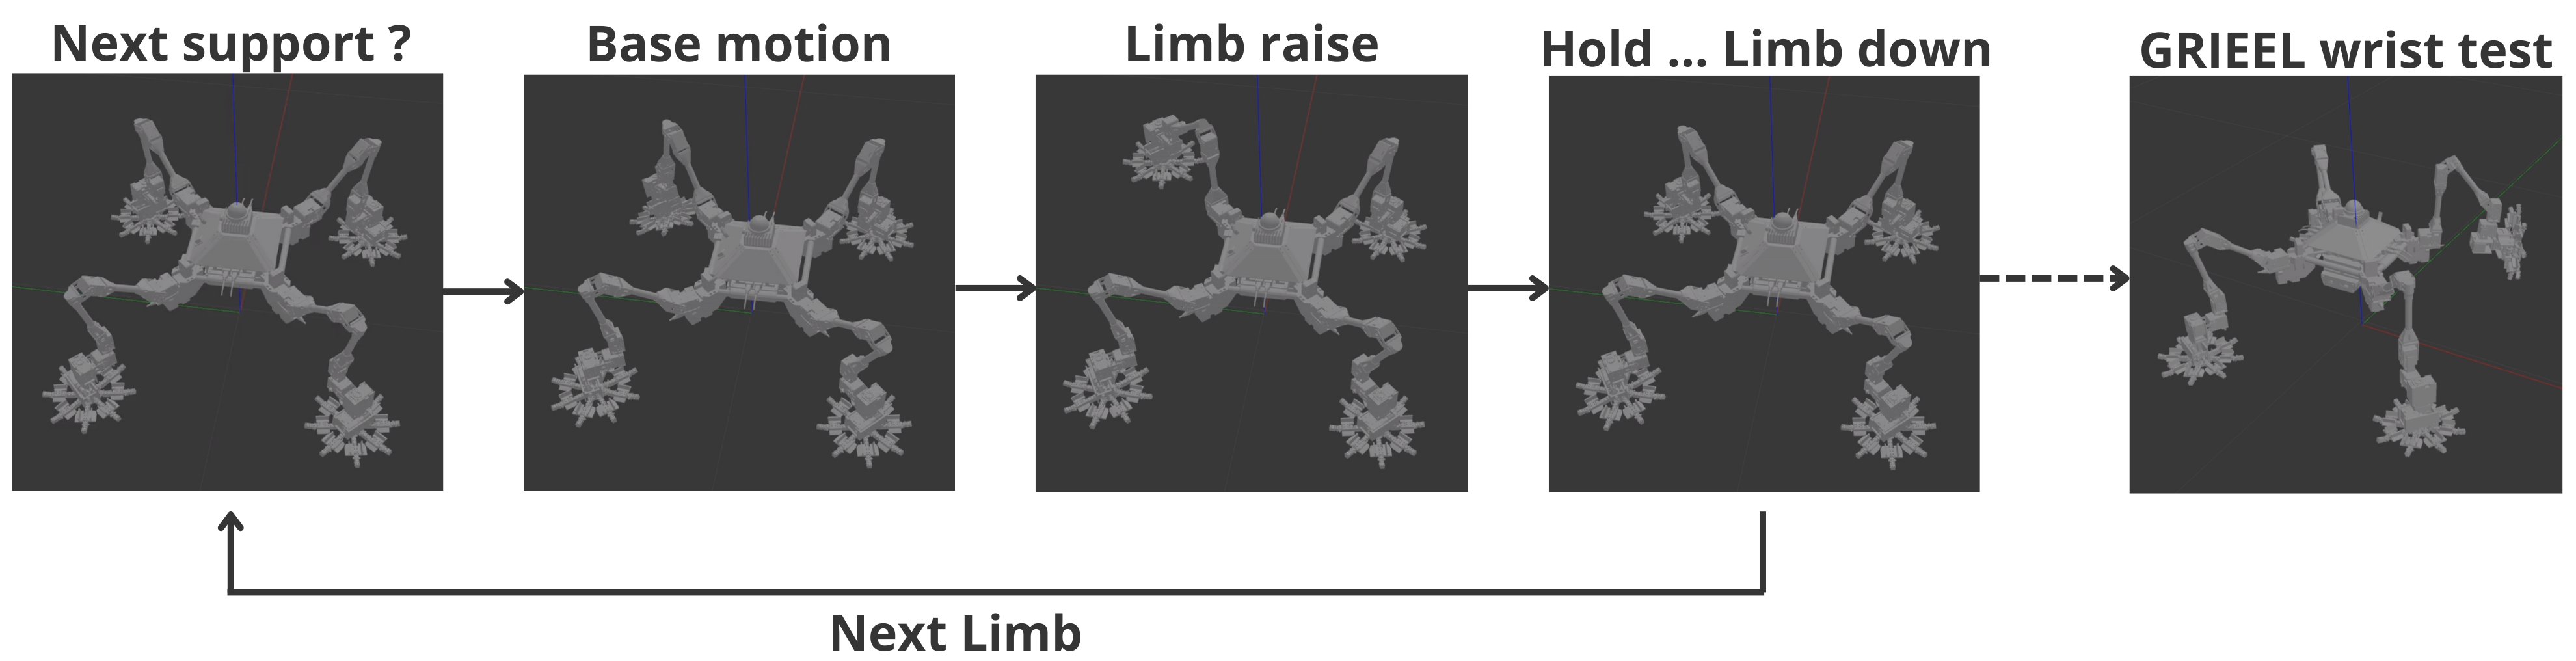
\includegraphics[width=0.95\textwidth]{Images/img_ch8/G2W_gazebo_classic.png}
    \caption{G2W motion sequence in Gazebo Classic}
    \label{fig:G2W_gazebo_classic}
\end{figure}

\begin{figure}[H]
    \centering
    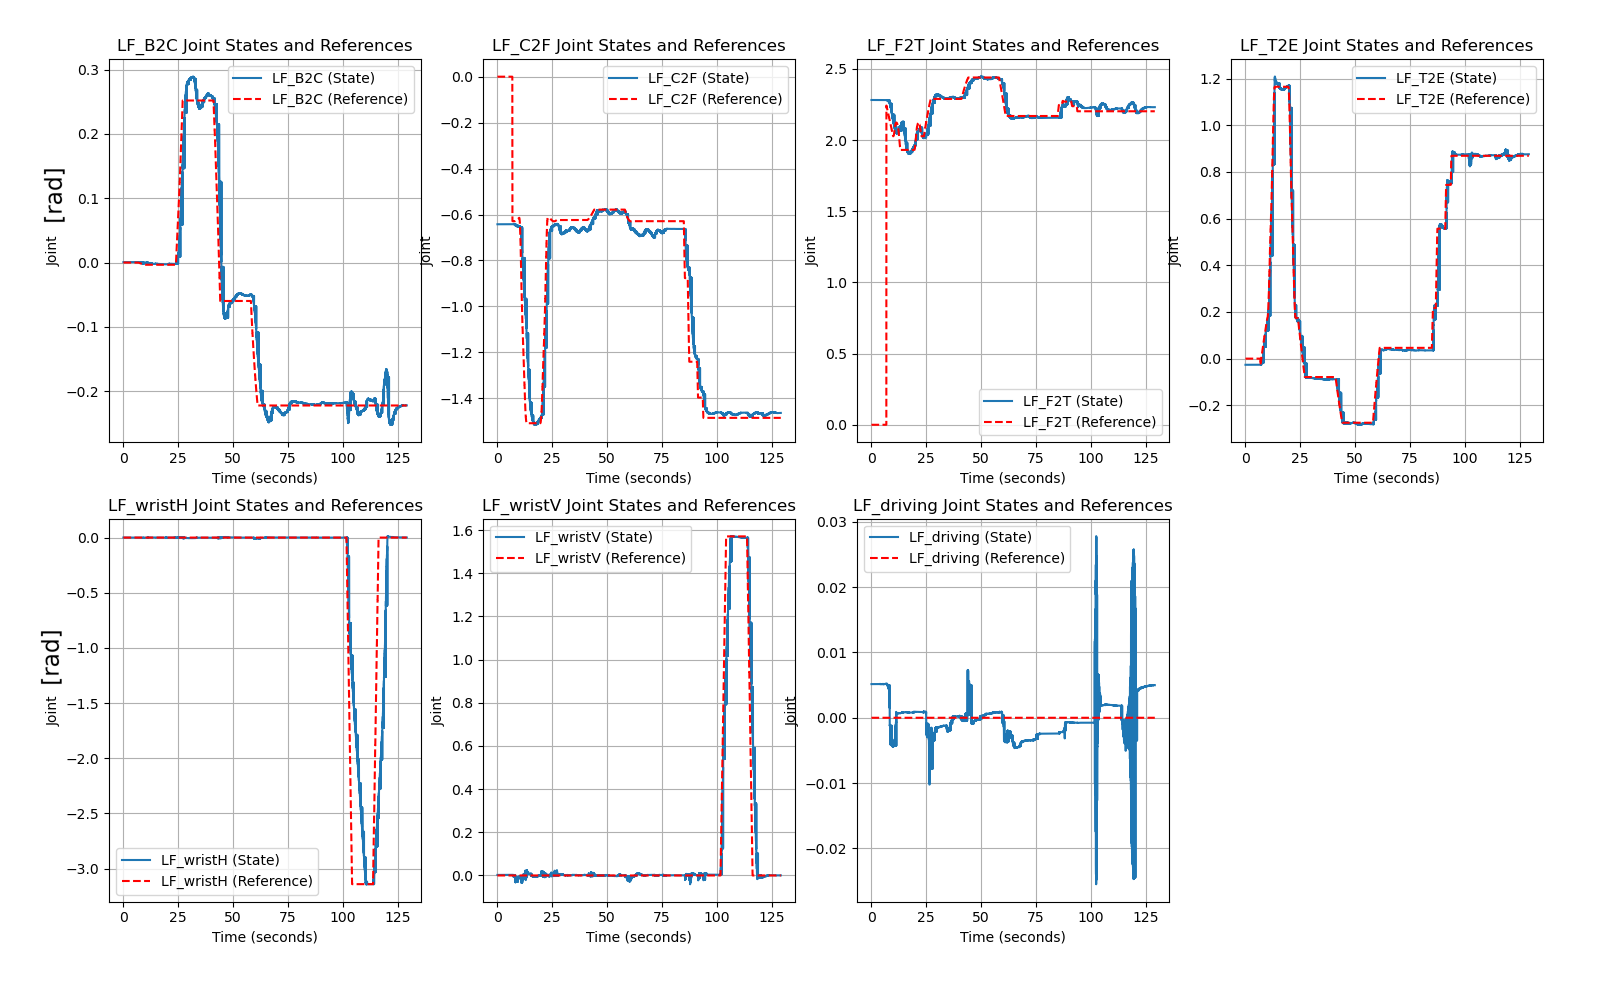
\includegraphics[width=0.90\textwidth]{Images/img_ch8/LF_Joints_PID.png}
    \caption{Joint tracking performance for LF limb, with JTC in Gazebo Classic}
    \label{fig:tracking_gz_classic}
\end{figure}

\section{Experiments Results}
\label{sec:exp_result}

Several transformation experiments on the real system have been conducted, from different initial limb configurations and GRIEEL mode, here a LF, LH, RH Gripper-to-Wheel transformation (with the algorithm defined in Chapter \ref{ch:chapter_five}) is reported. 

In Fig.\ref{fig:exp_seq} the time-lapse is represented, and the corresponding joint state tracking performance for each limb is shown in Figs.\ref{fig:LF_exp} - \ref{fig:RF_exp}. 

The results on stability and dexterity measures are respectively in Fig.\ref{fig:SSM}, and Figs.\ref{fig:LF_manipulability},\ref{fig:LH_RH_manipulability}.

\begin{figure}[H]
    \centering
    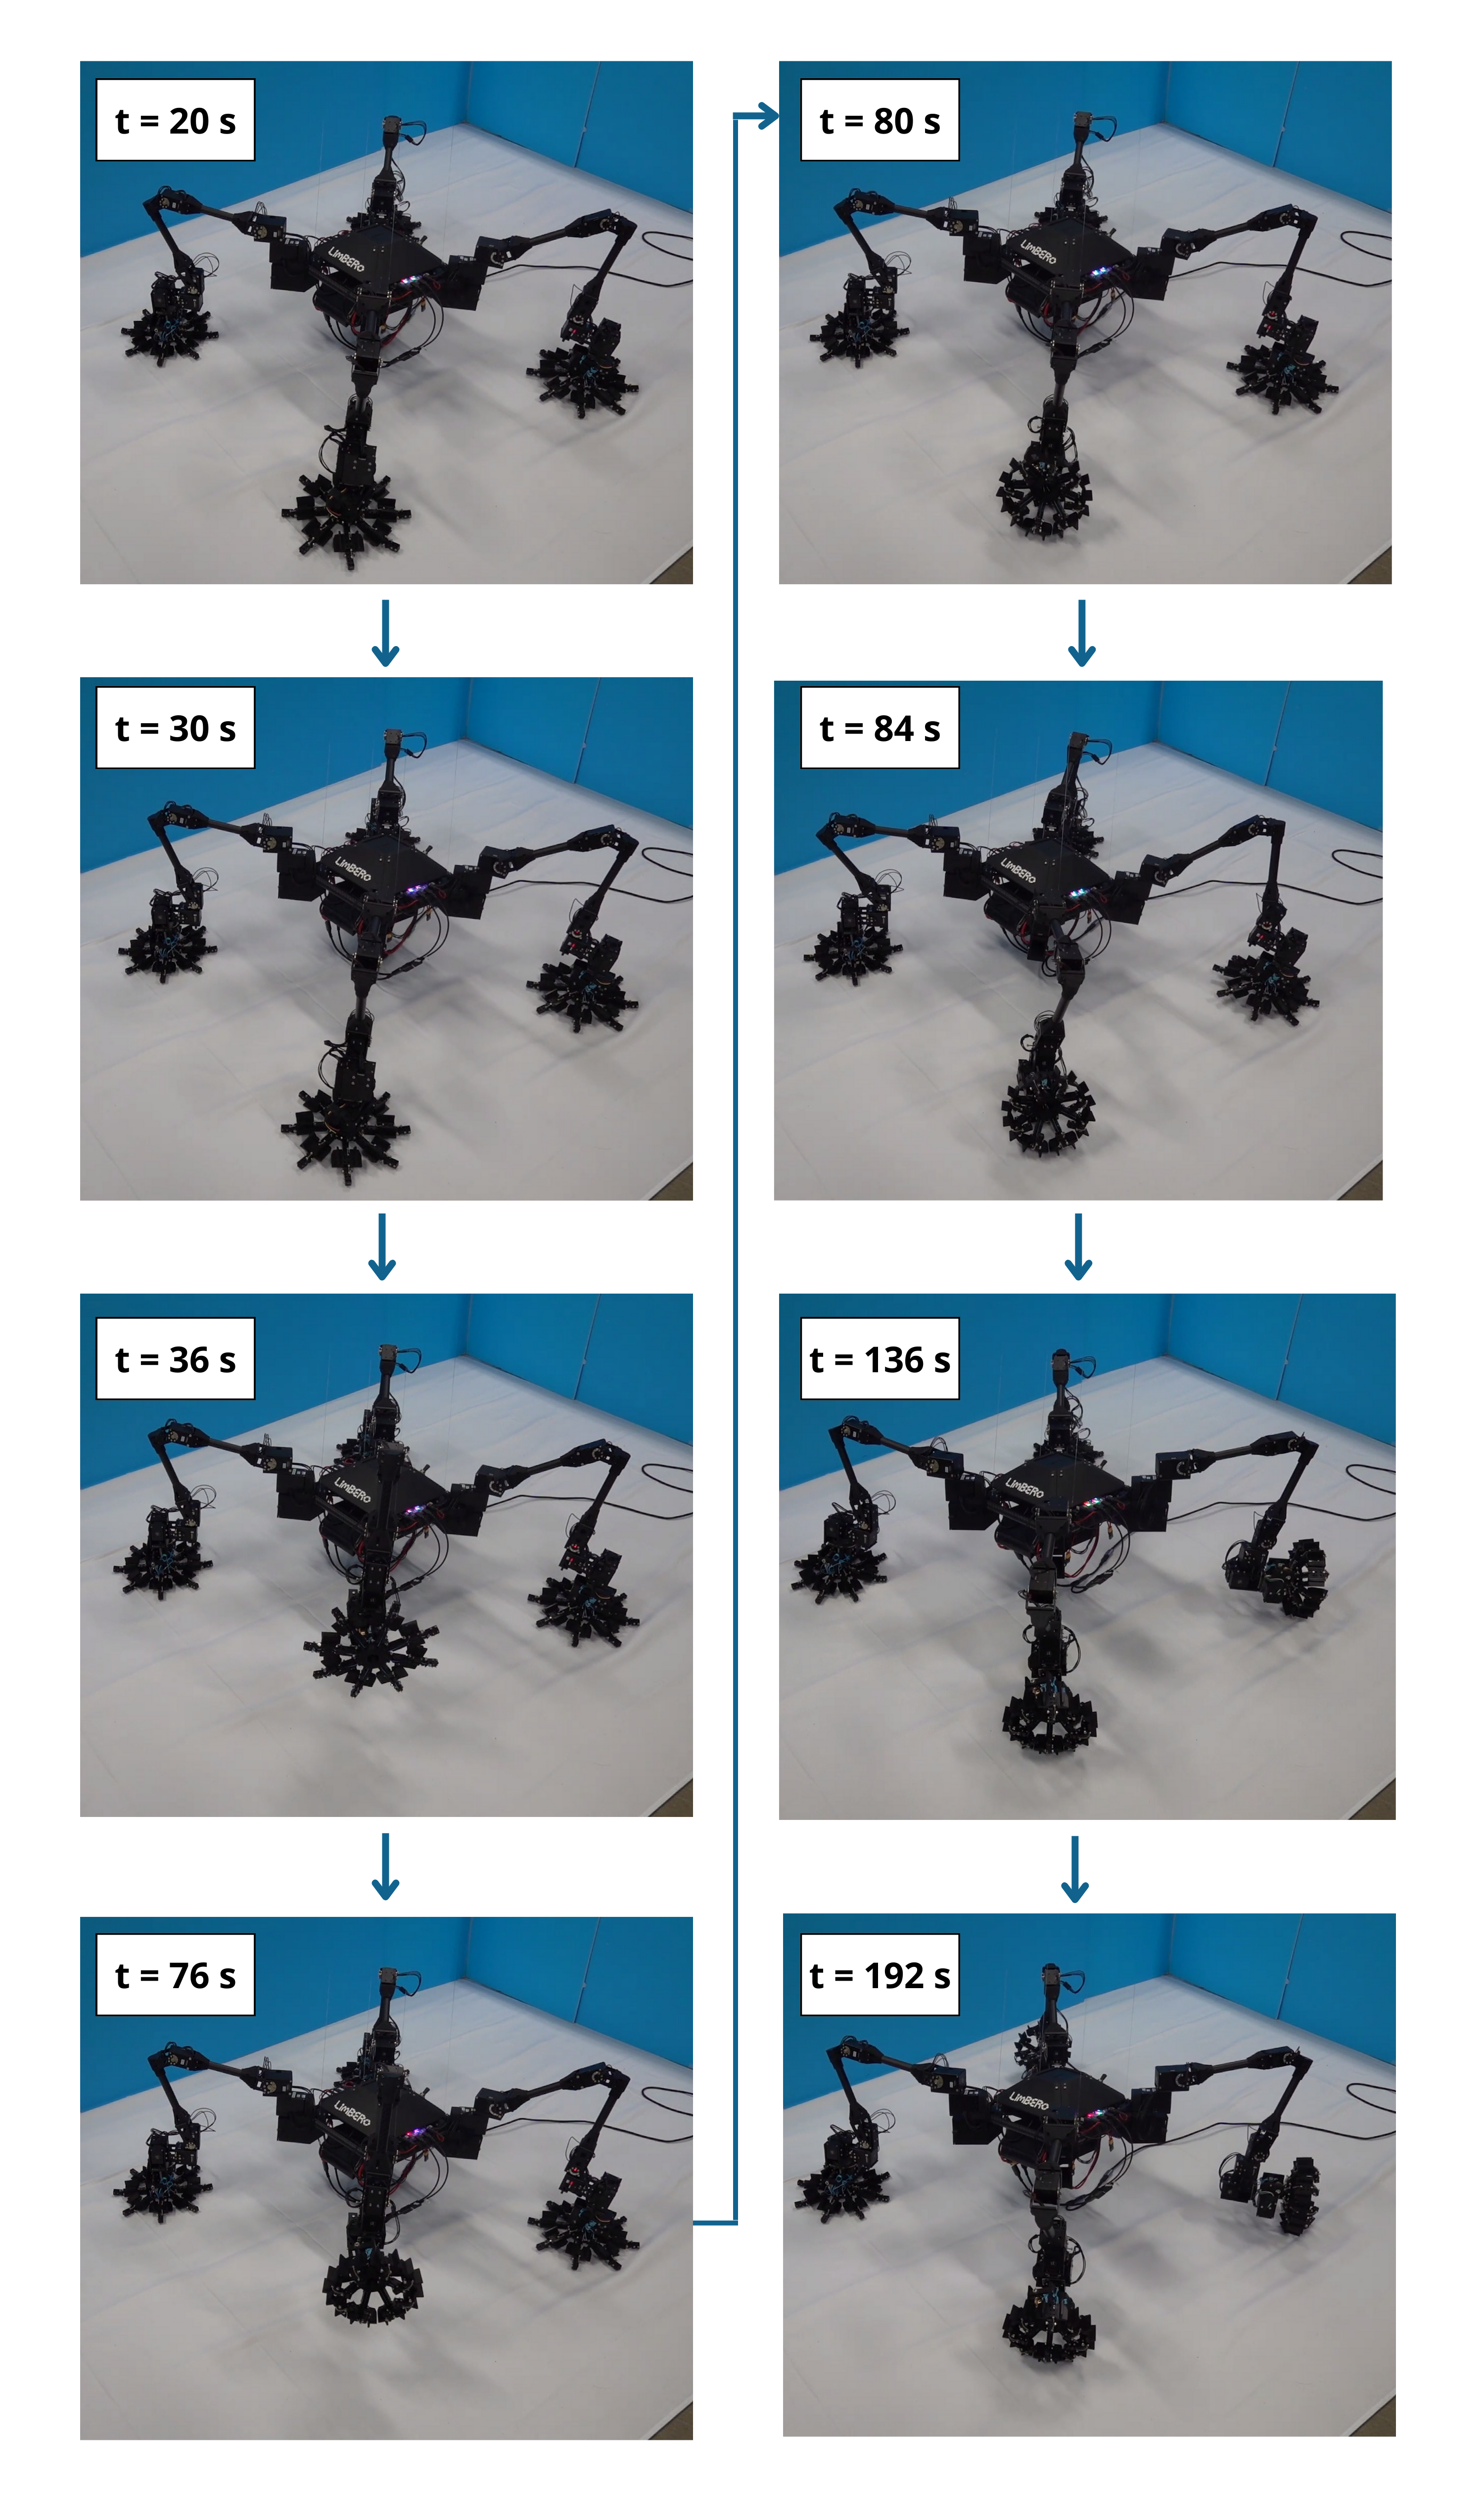
\includegraphics[width=0.6\textwidth]{Images/img_ch8/experiment_sequence.png}
    \caption{G2W Experiment time-lapse (LF, LH, RH)}
    \label{fig:exp_seq}
\end{figure}

\begin{figure}[H]
    \centering
    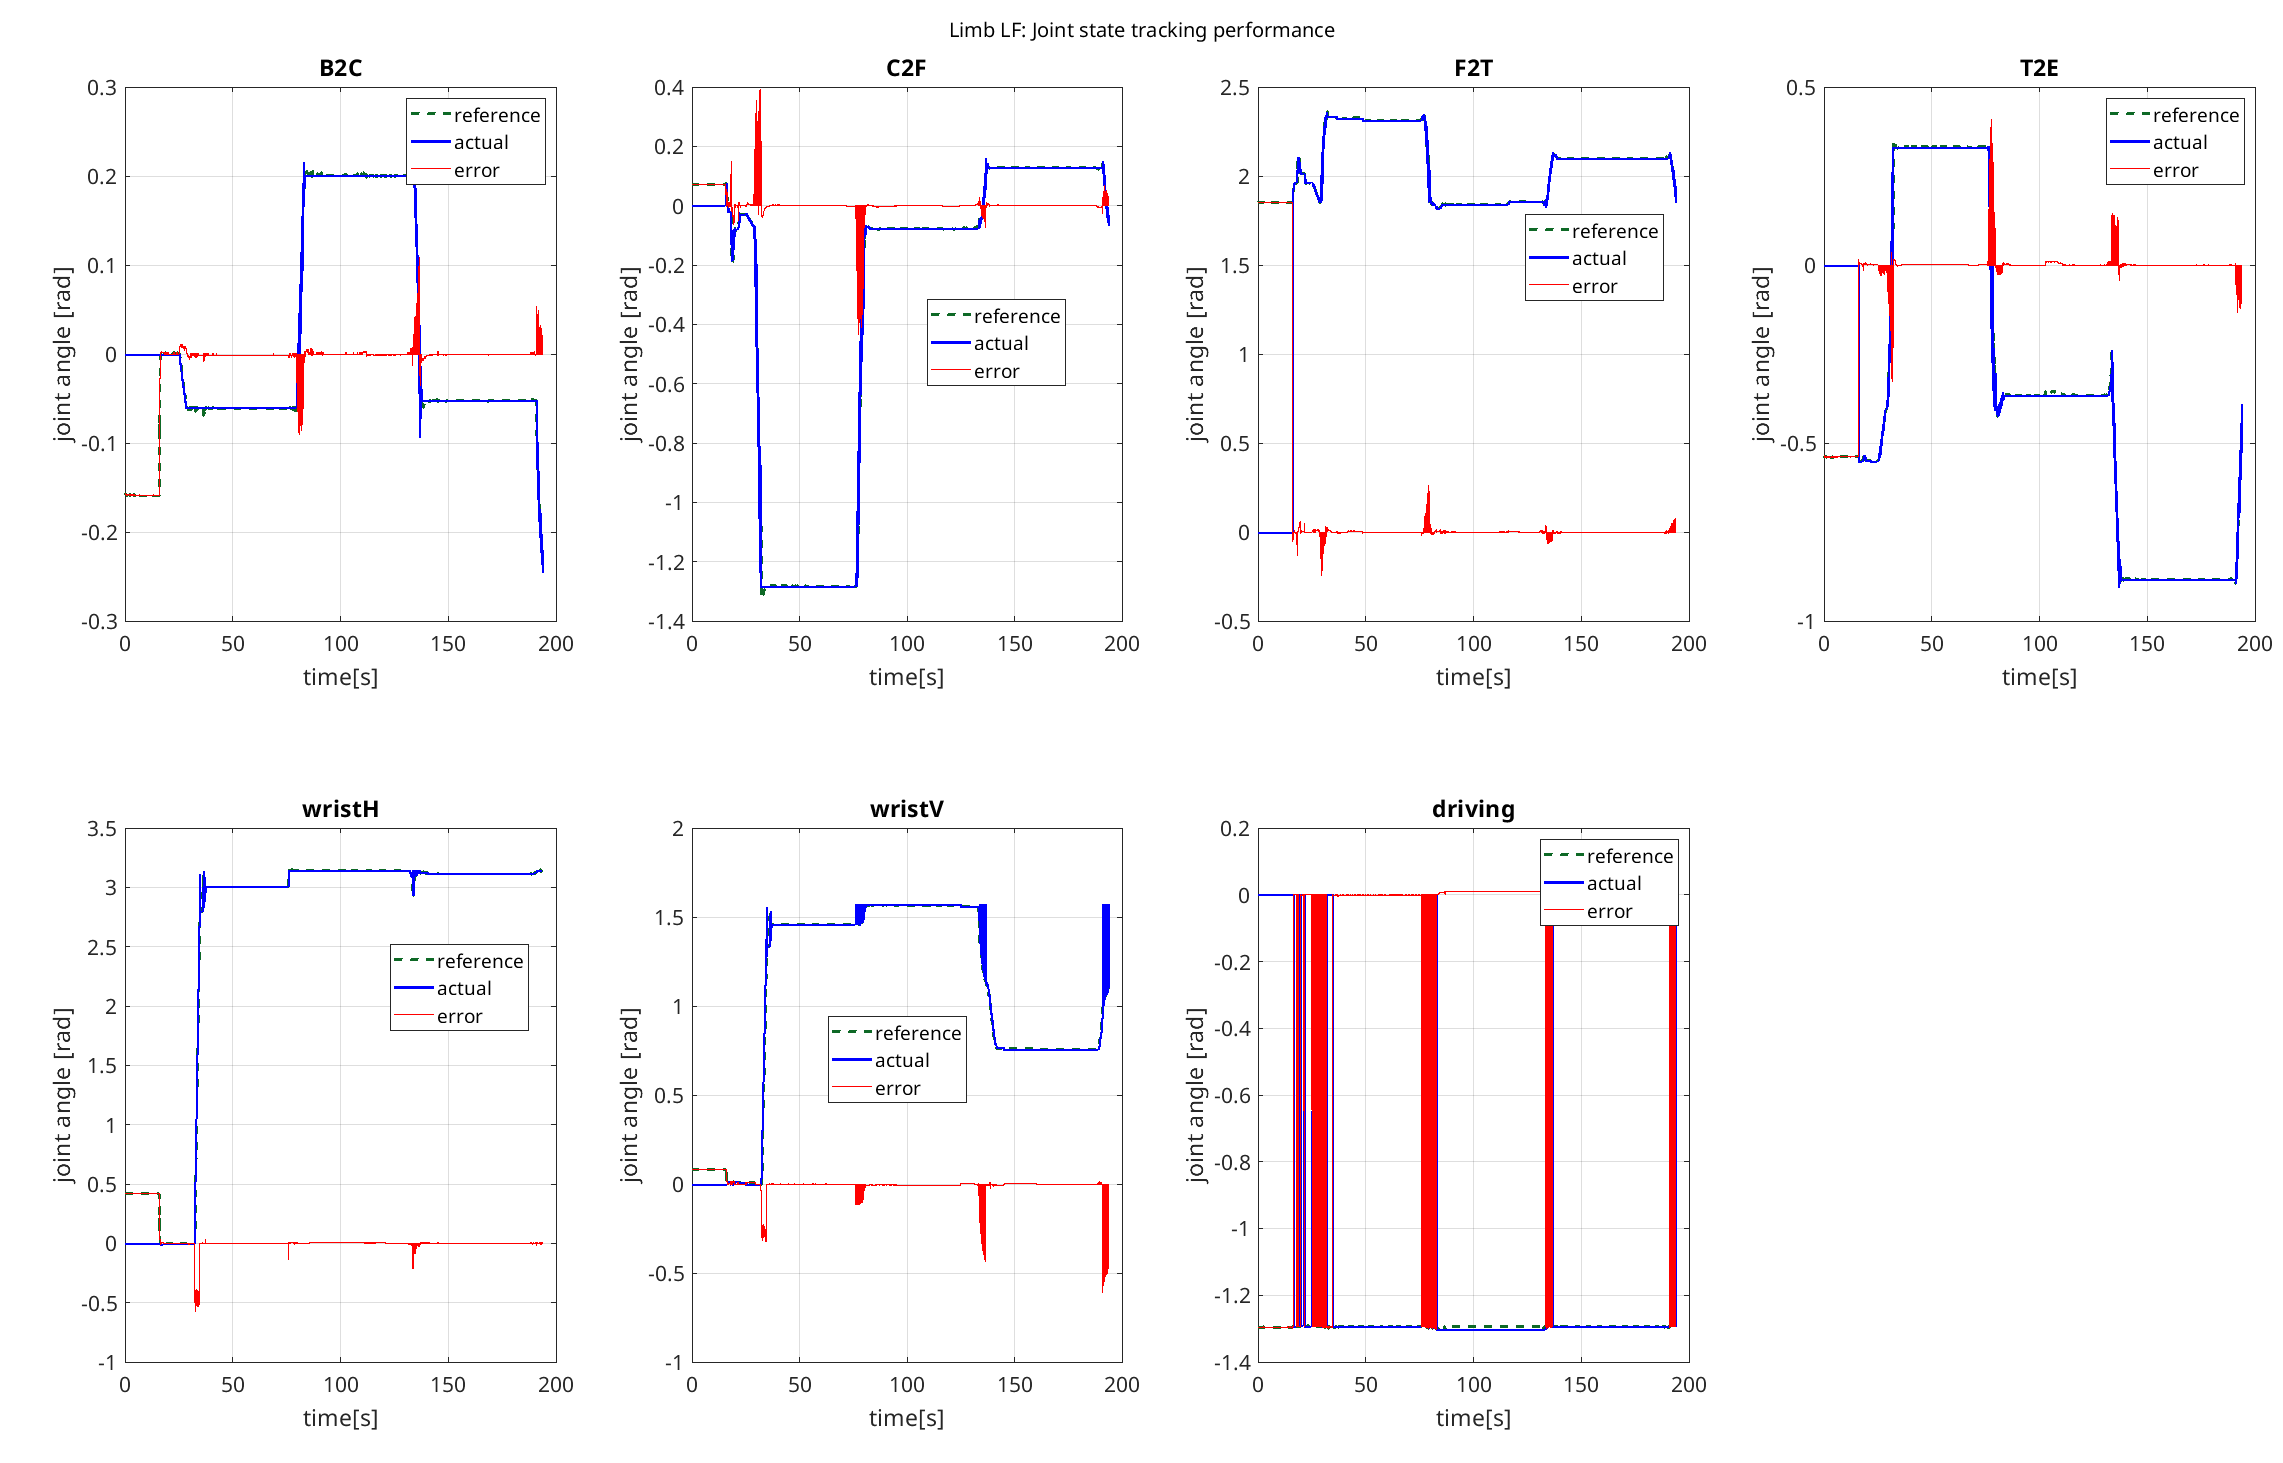
\includegraphics[width=1.0\textwidth]{Images/img_ch8/LF_experiment.png}
    \caption{LF limb, Joint tracking performance during G2W experiment}
    \label{fig:LF_exp}
\end{figure}

\begin{figure}[H]
    \centering
    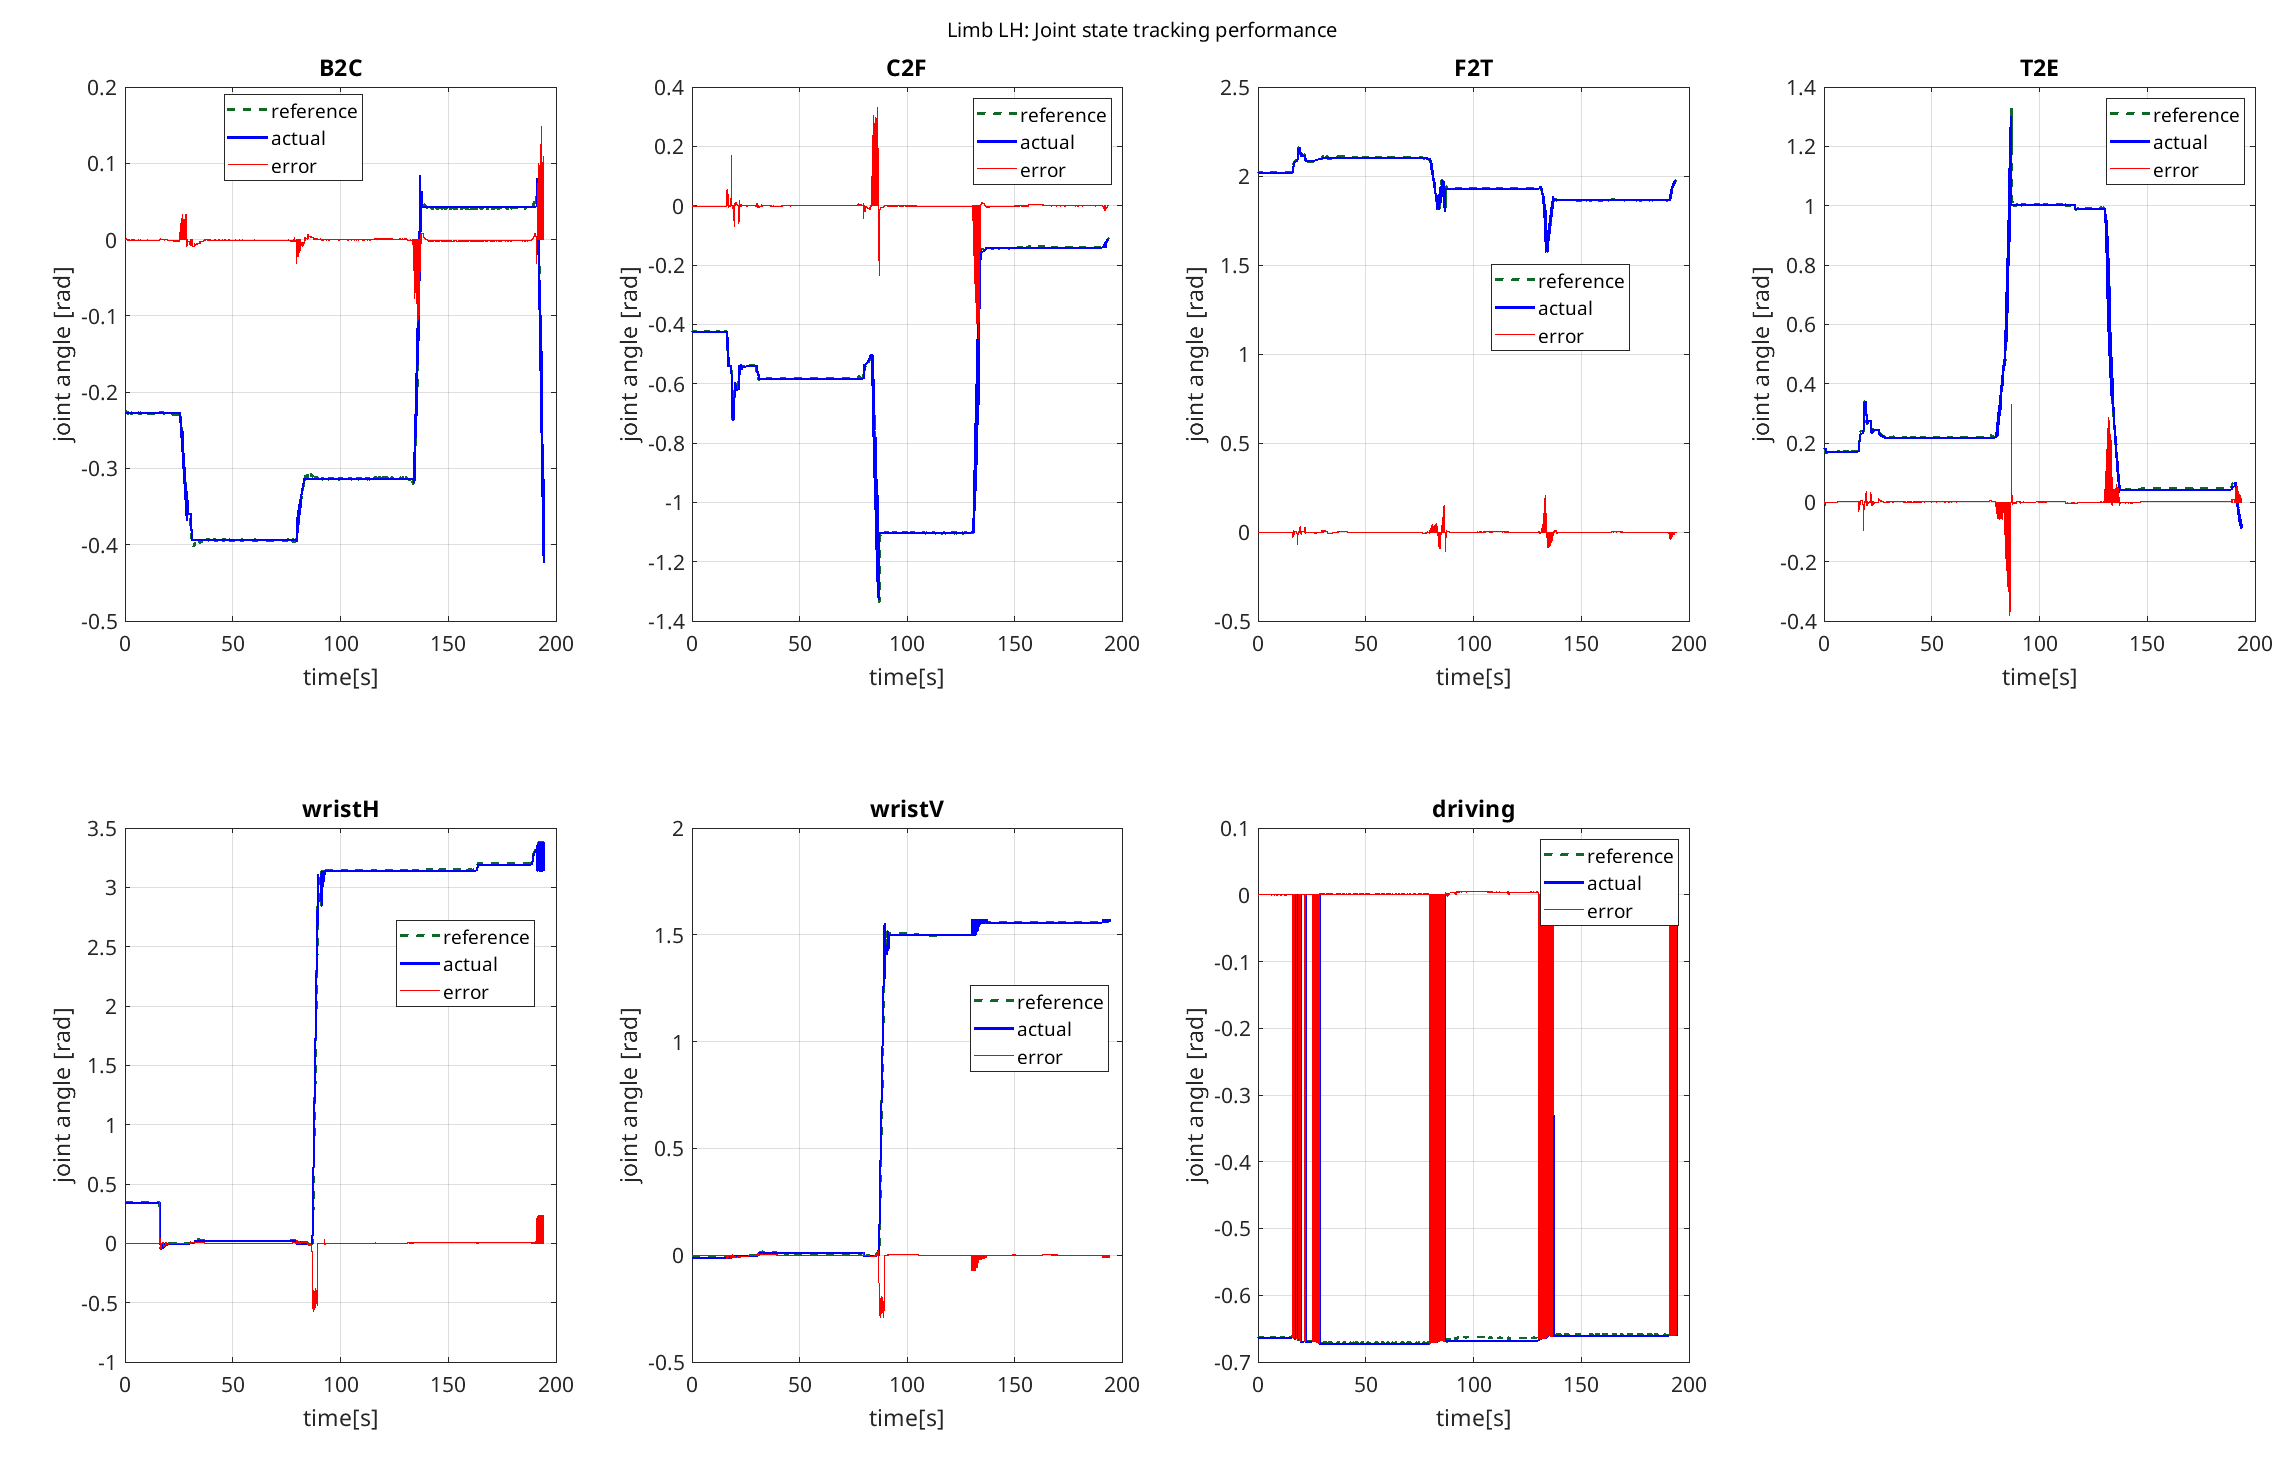
\includegraphics[width=1.0\textwidth]{Images/img_ch8/LH_experiment.png}
    \caption{LH limb, Joint tracking performance during G2W experiment}
    \label{fig:LH_exp}
\end{figure}

\begin{figure}[H]
    \centering
    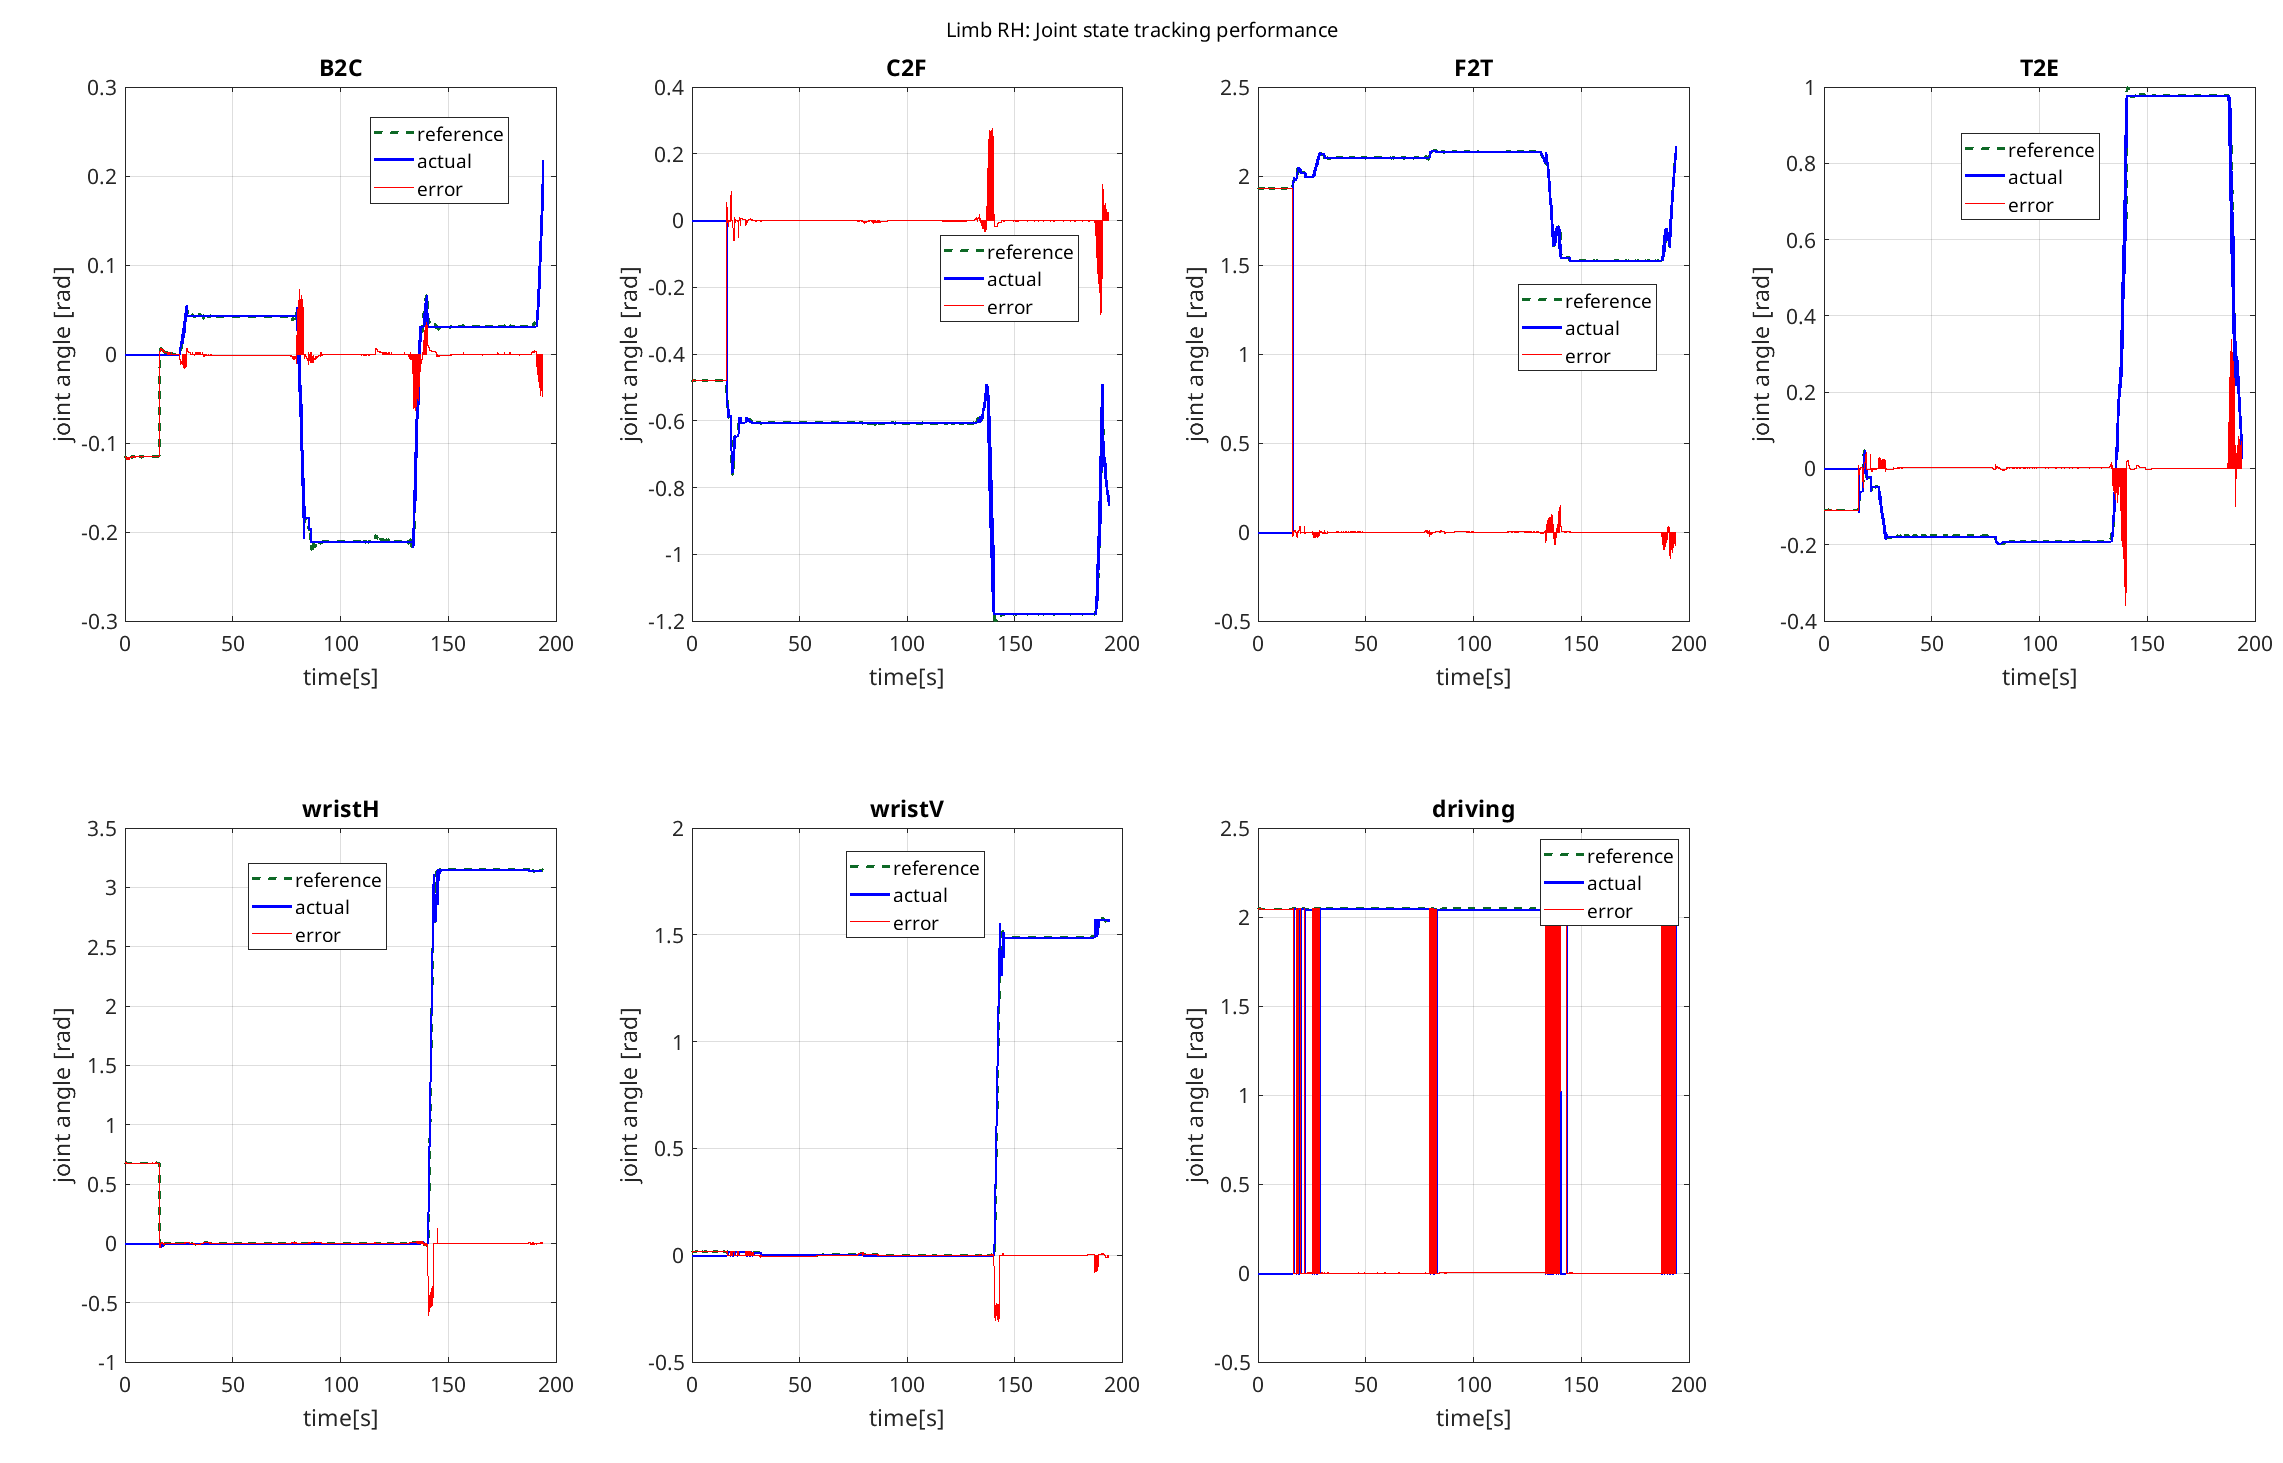
\includegraphics[width=1.0\textwidth]{Images/img_ch8/RH_experiment.png}
    \caption{RH limb, Joint tracking performance during G2W experiment}
    \label{fig:RH_exp}
\end{figure}

\begin{figure}[H]
    \centering
    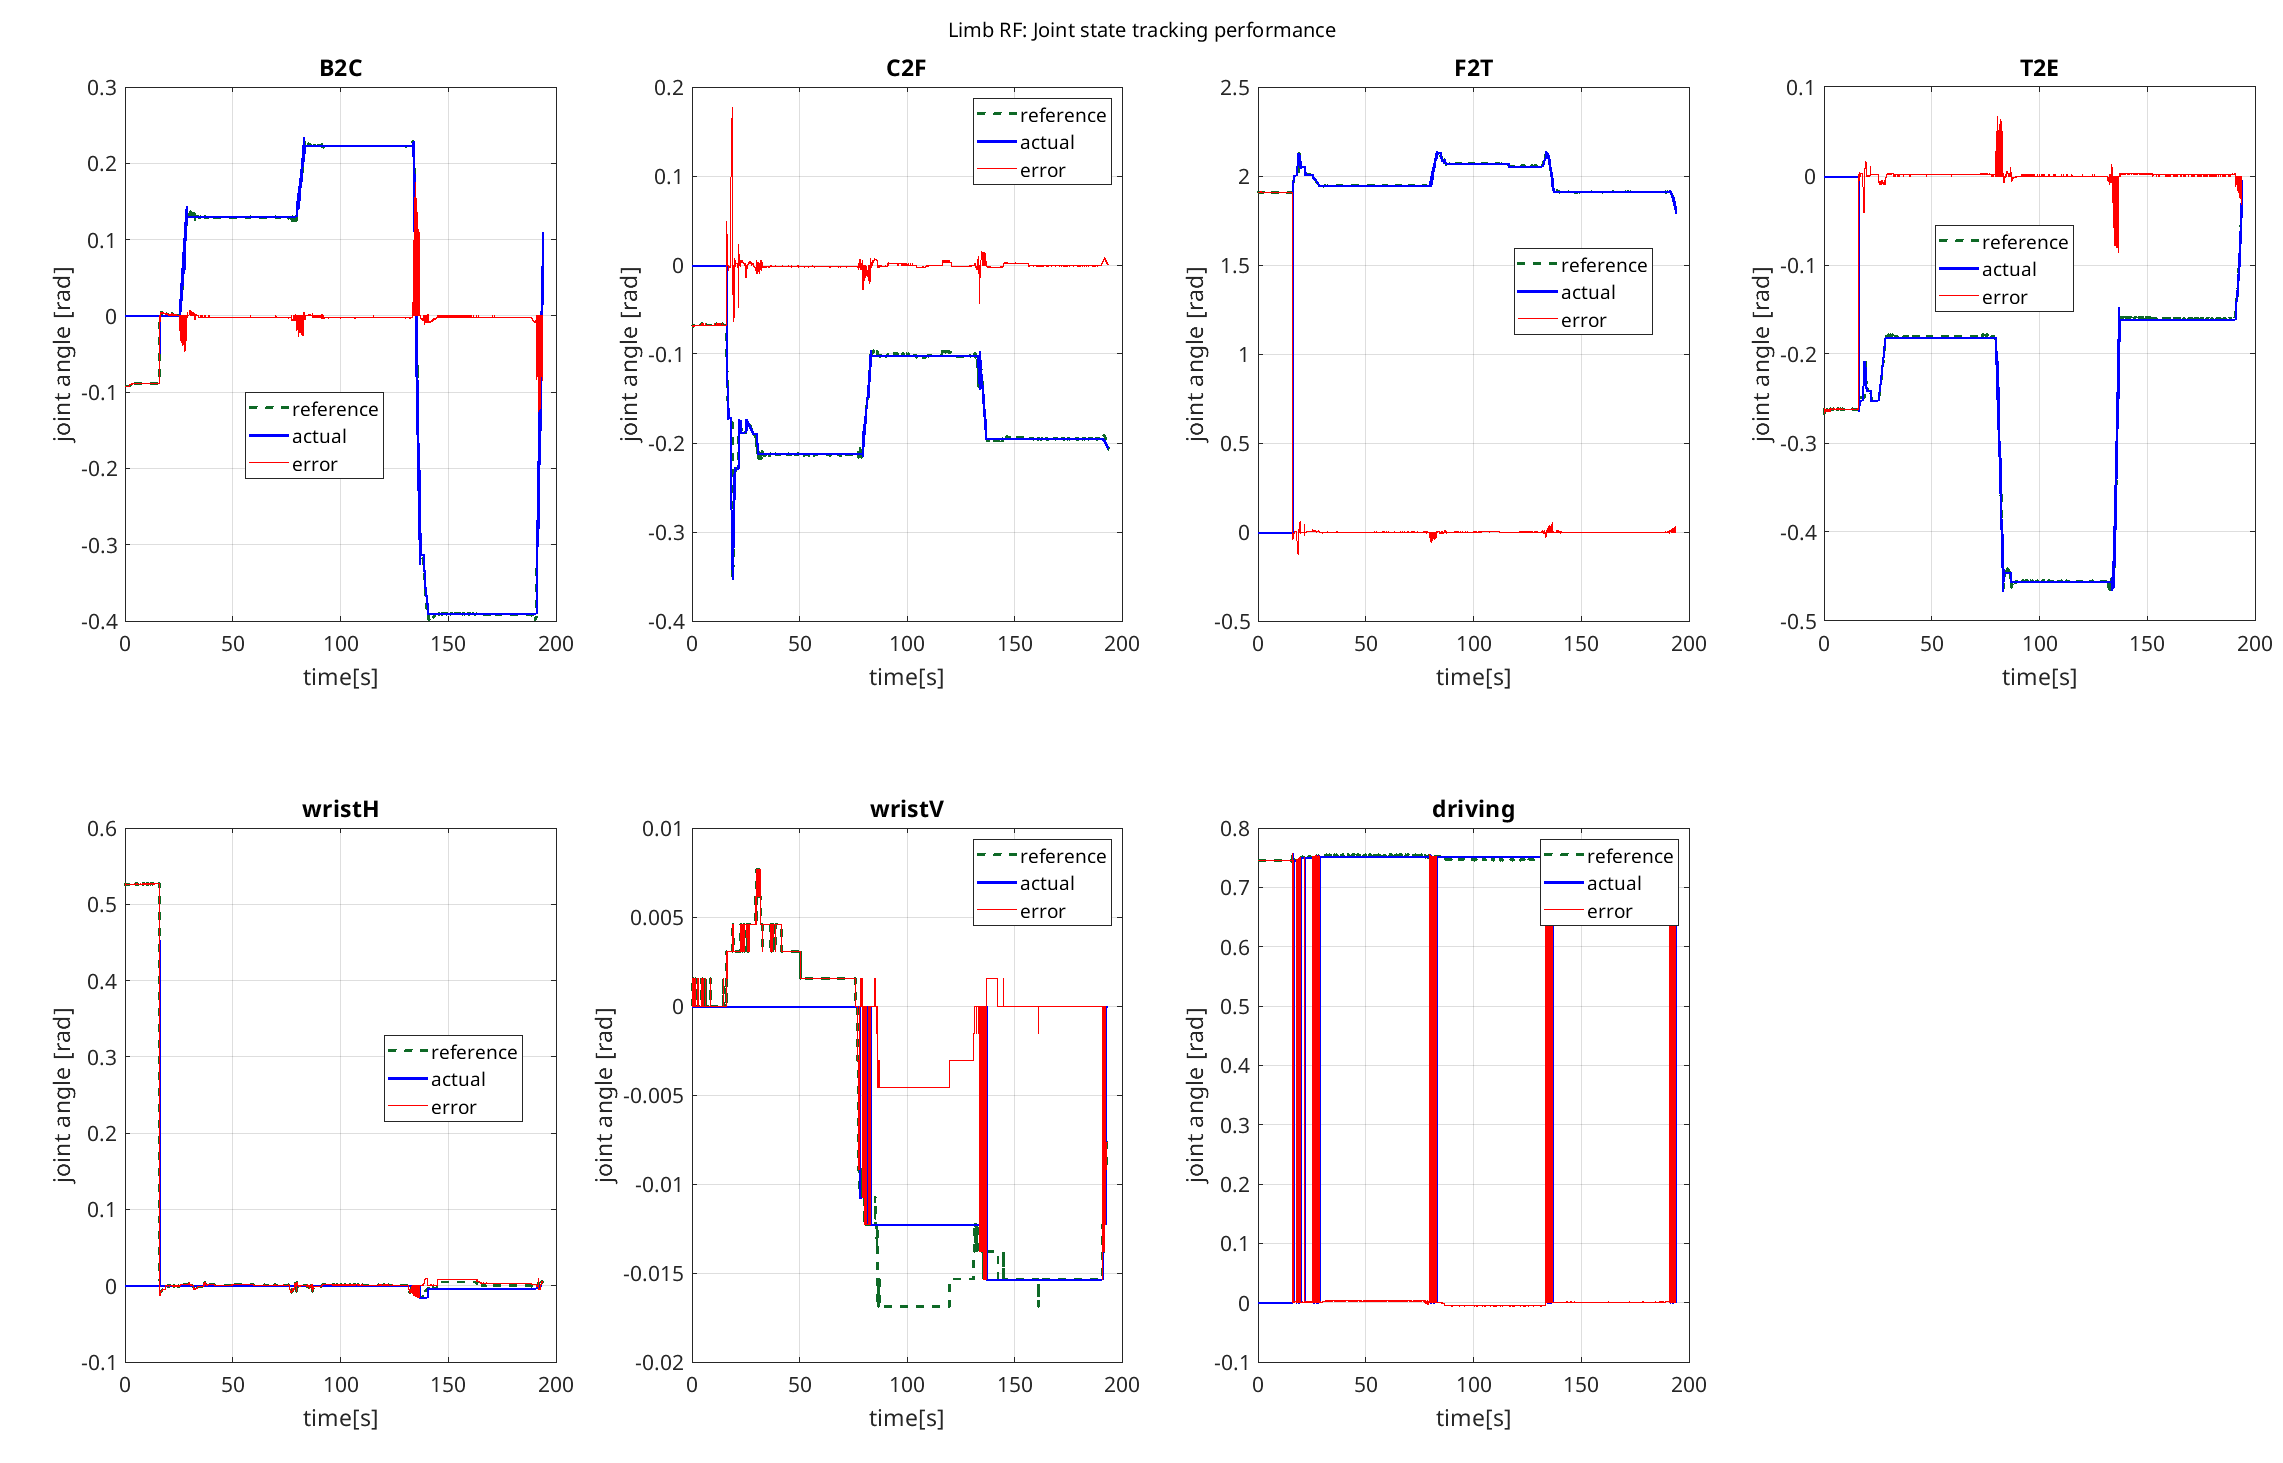
\includegraphics[width=1.0\textwidth]{Images/img_ch8/RF_experiment.png}
    \caption{RF limb, Joint tracking performance during G2W experiment}
    \label{fig:RF_exp}
\end{figure}

\begin{figure}[H]
    \centering
    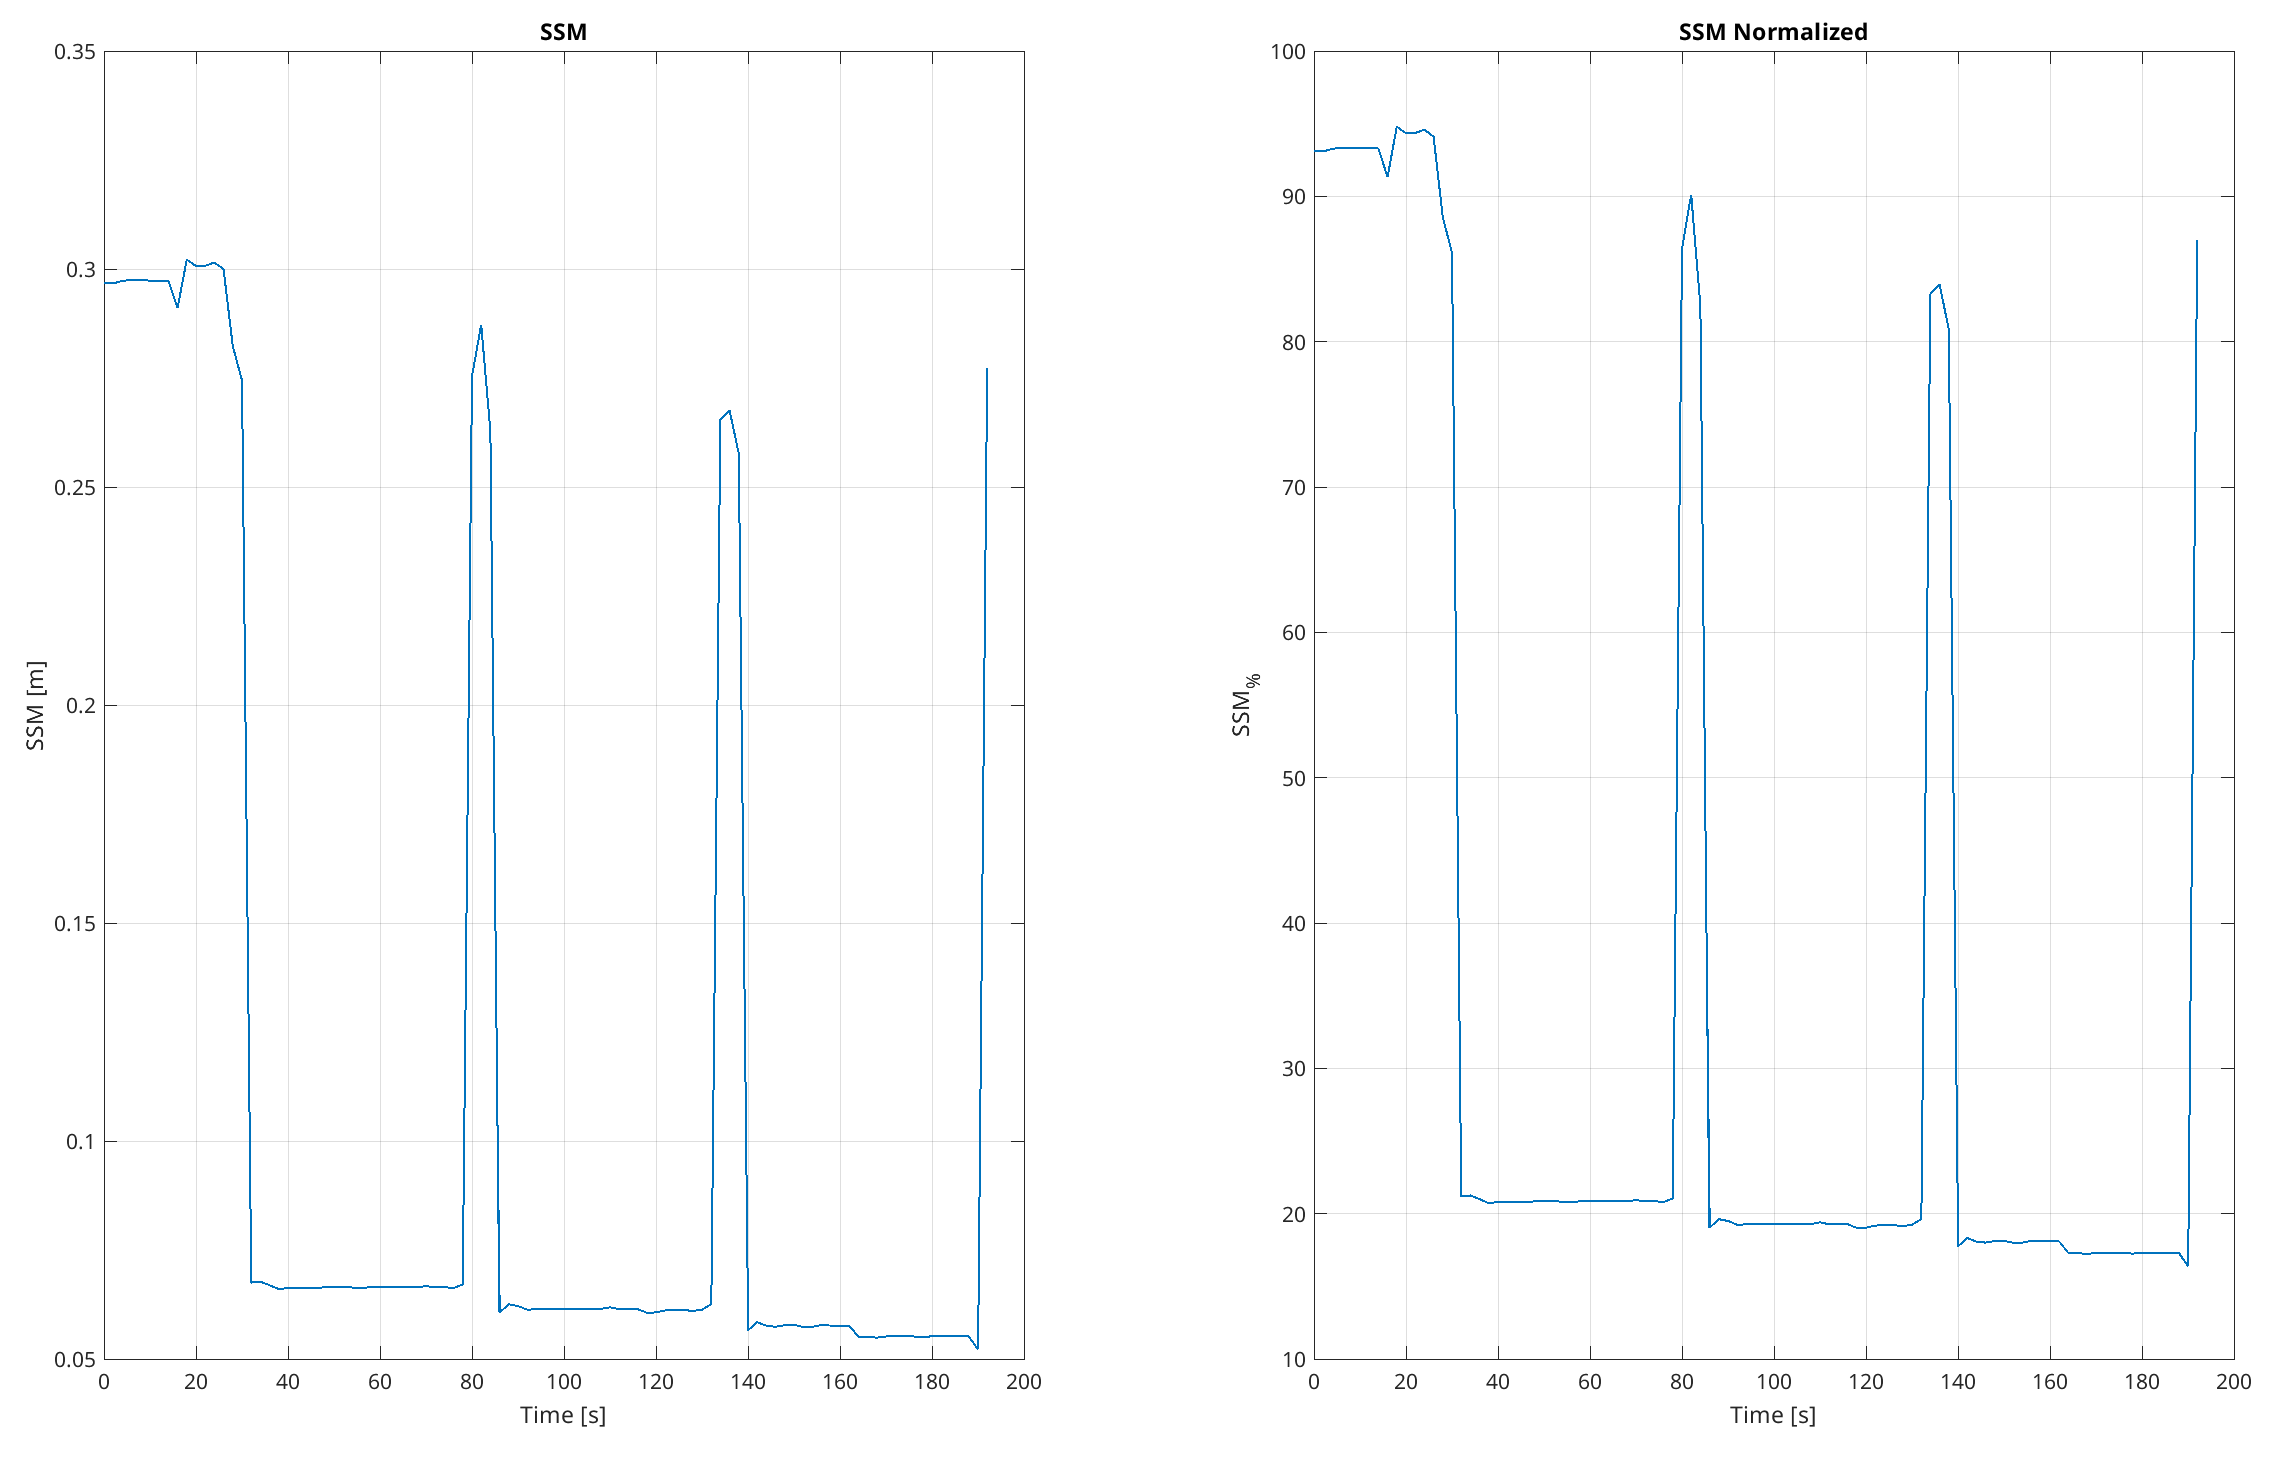
\includegraphics[width=0.9\textwidth]{Images/img_ch8/SSM_experiment.png}
    \caption{SSM and normalized SSM during G2W transformation}
    \label{fig:SSM}
\end{figure}

\begin{figure}[H]
    \centering
    \subfloat[Initial configuration (t=20 s)\label{fig:step1}]{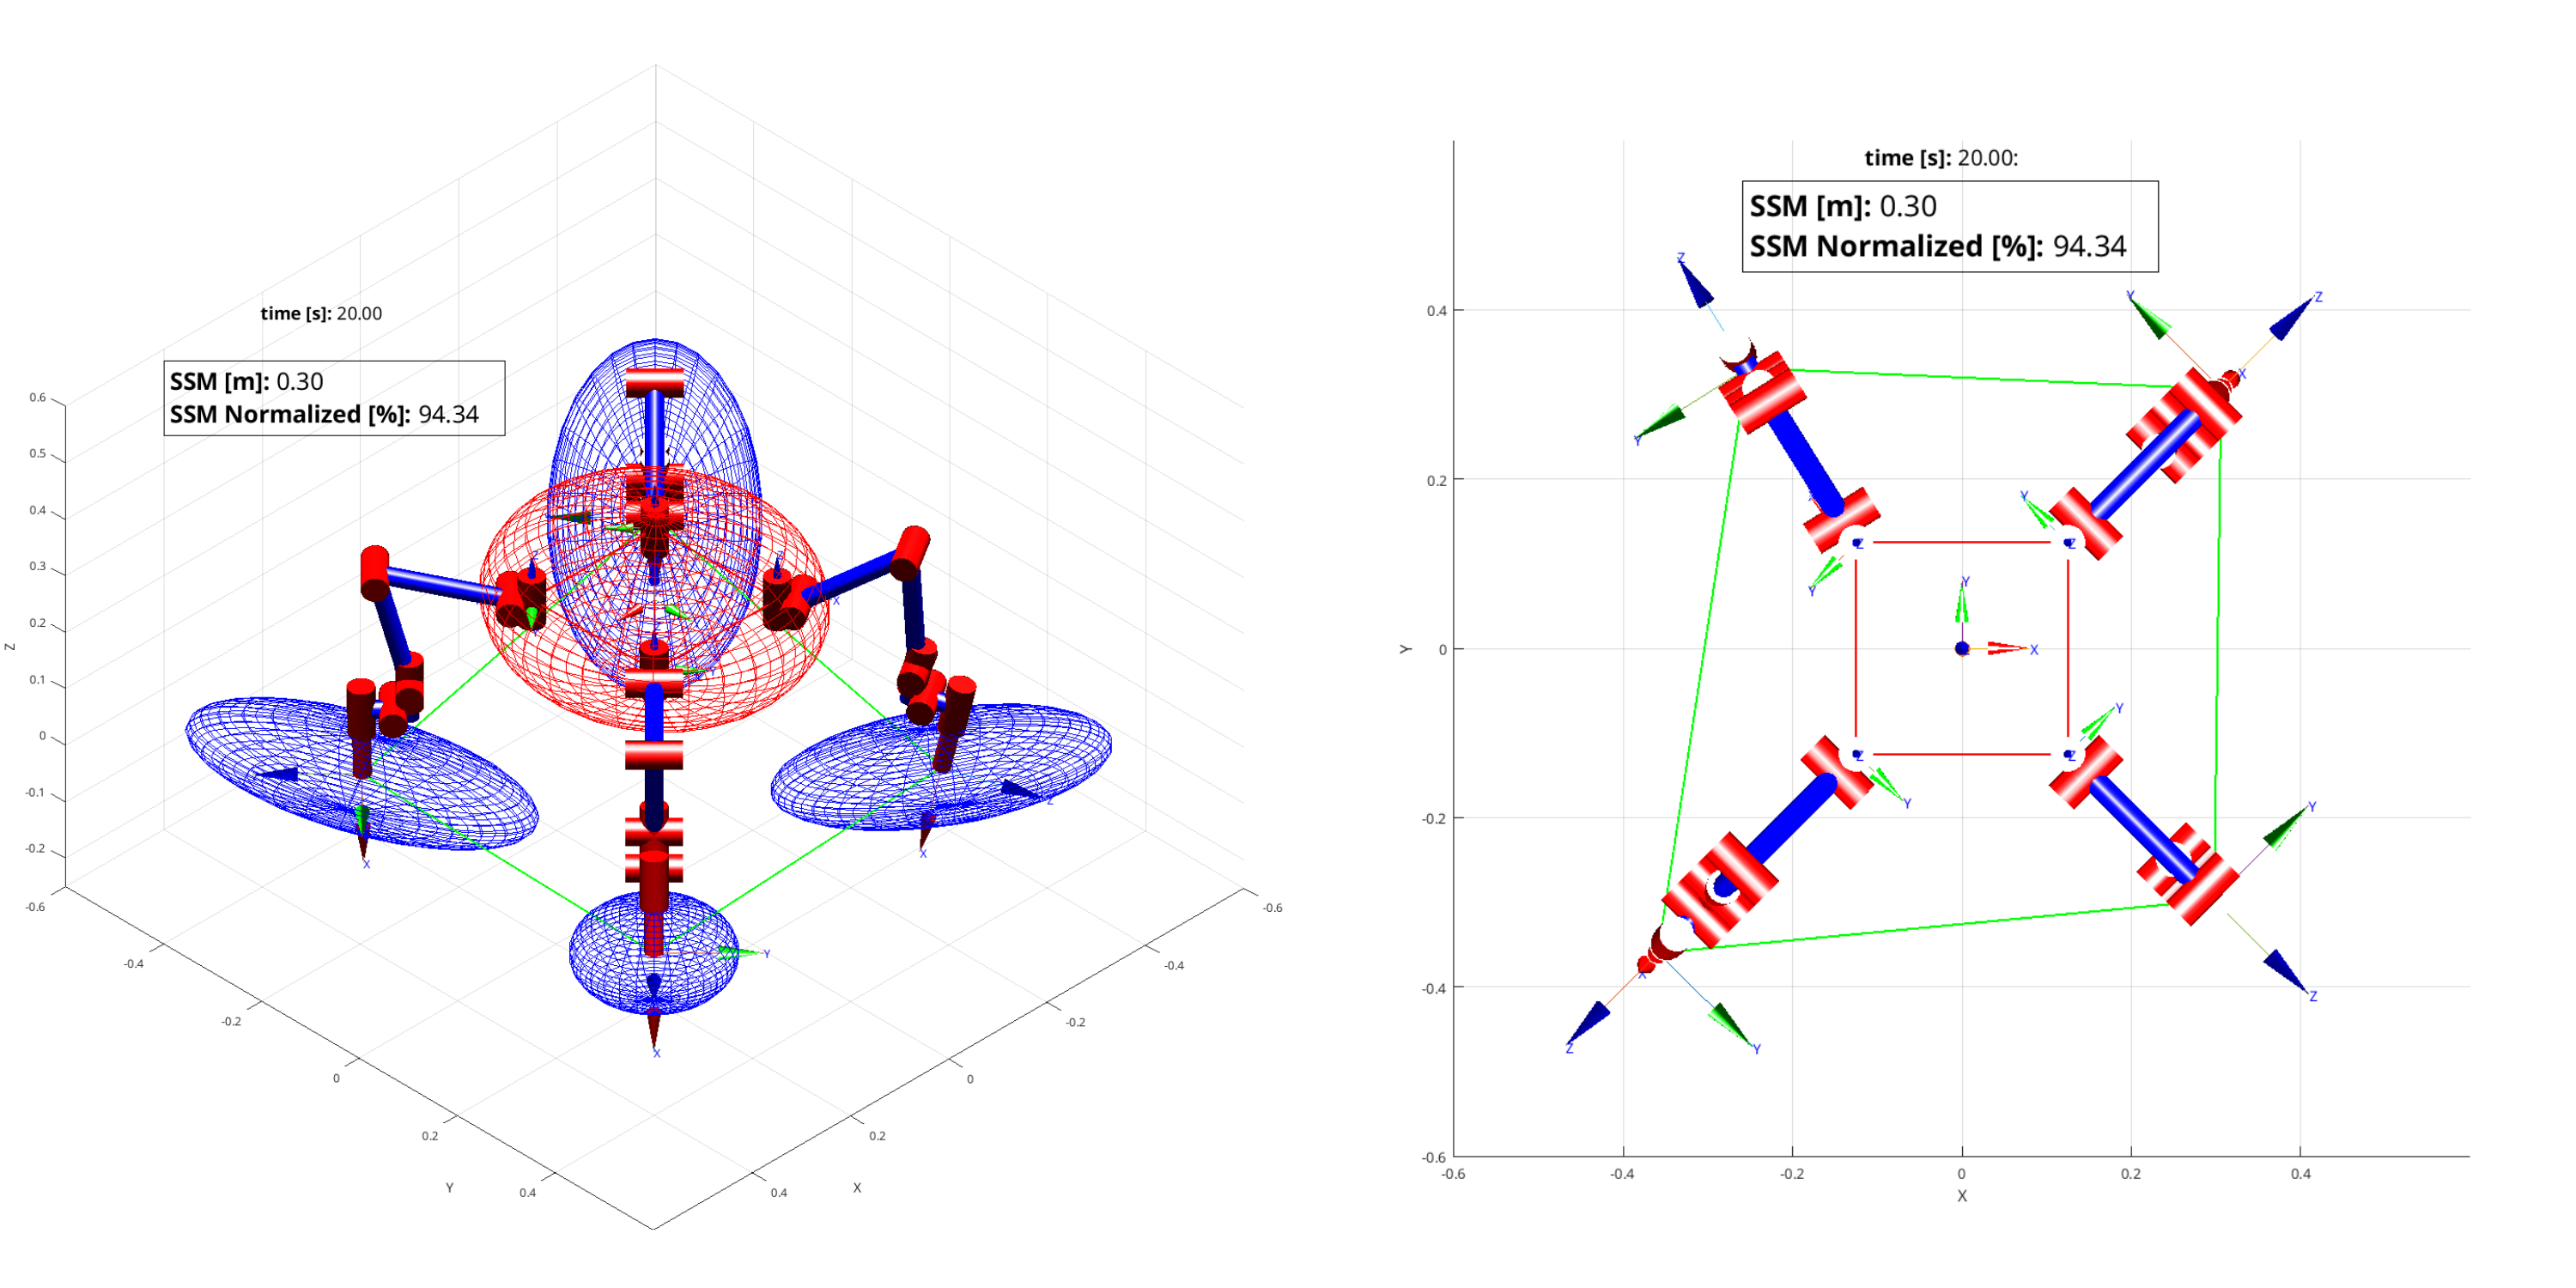
\includegraphics[width=0.55\textwidth]{Images/img_ch8/step1_exp.png}} 
    \subfloat[Base motion (t=30 s)\label{fig:step2}]{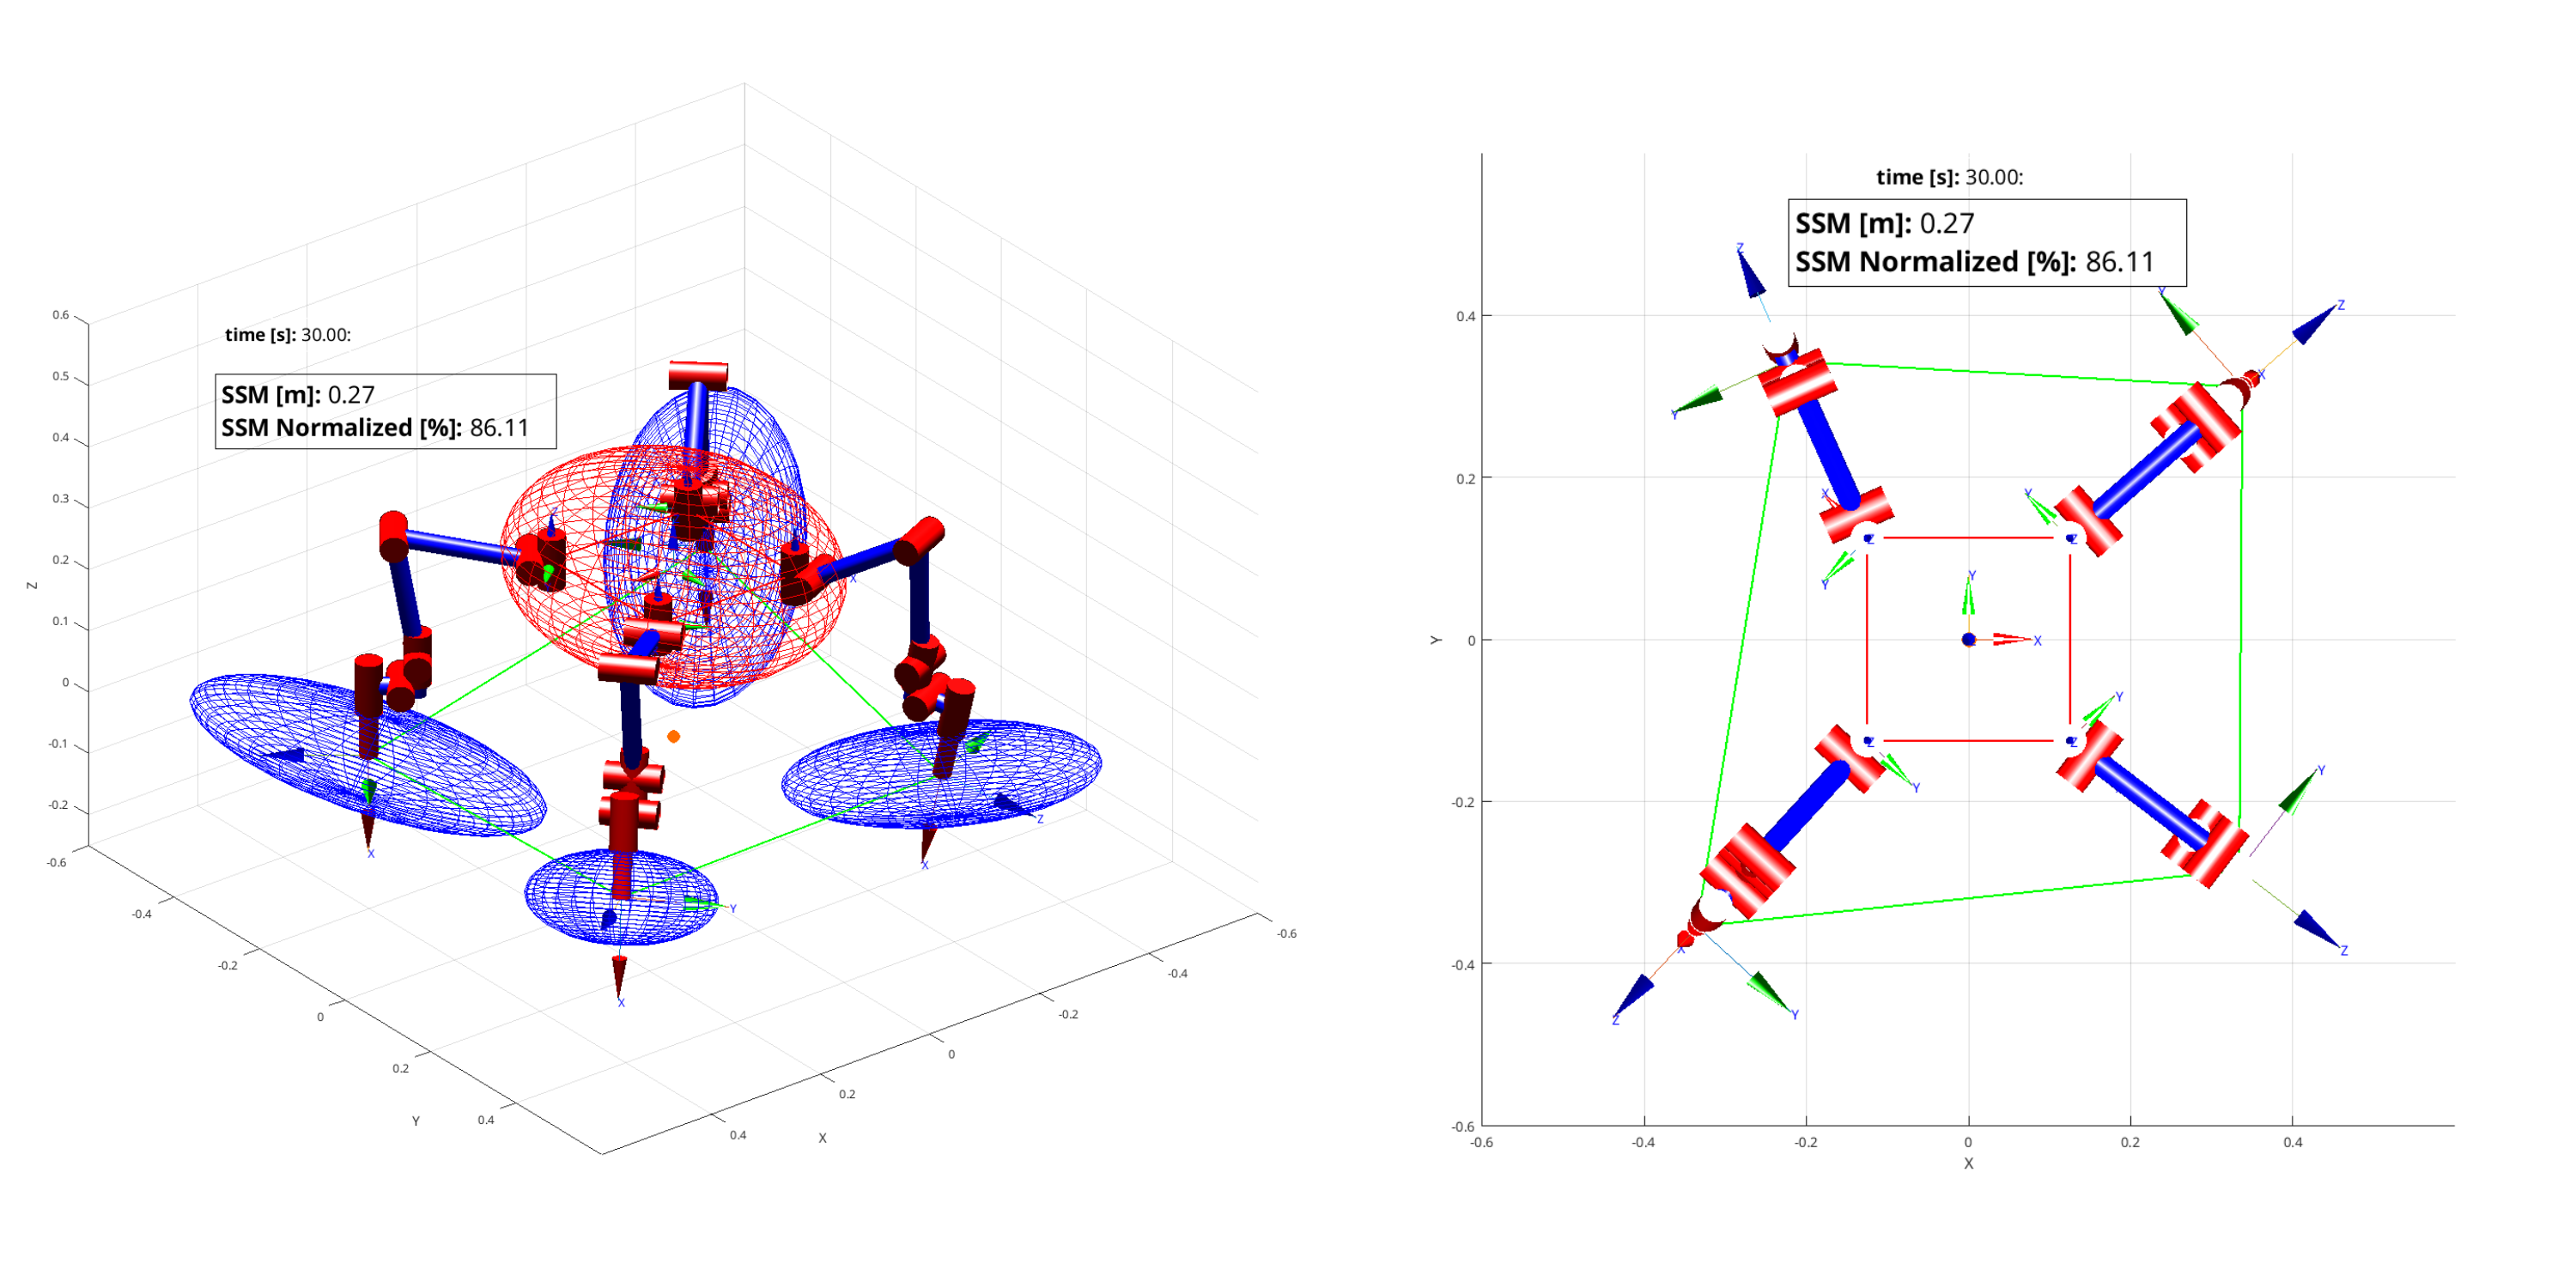
\includegraphics[width=0.55\textwidth]{Images/img_ch8/step2_exp.png}}\\ 

    \subfloat[LF Limb Raise (t=36 s)\label{fig:step3}]{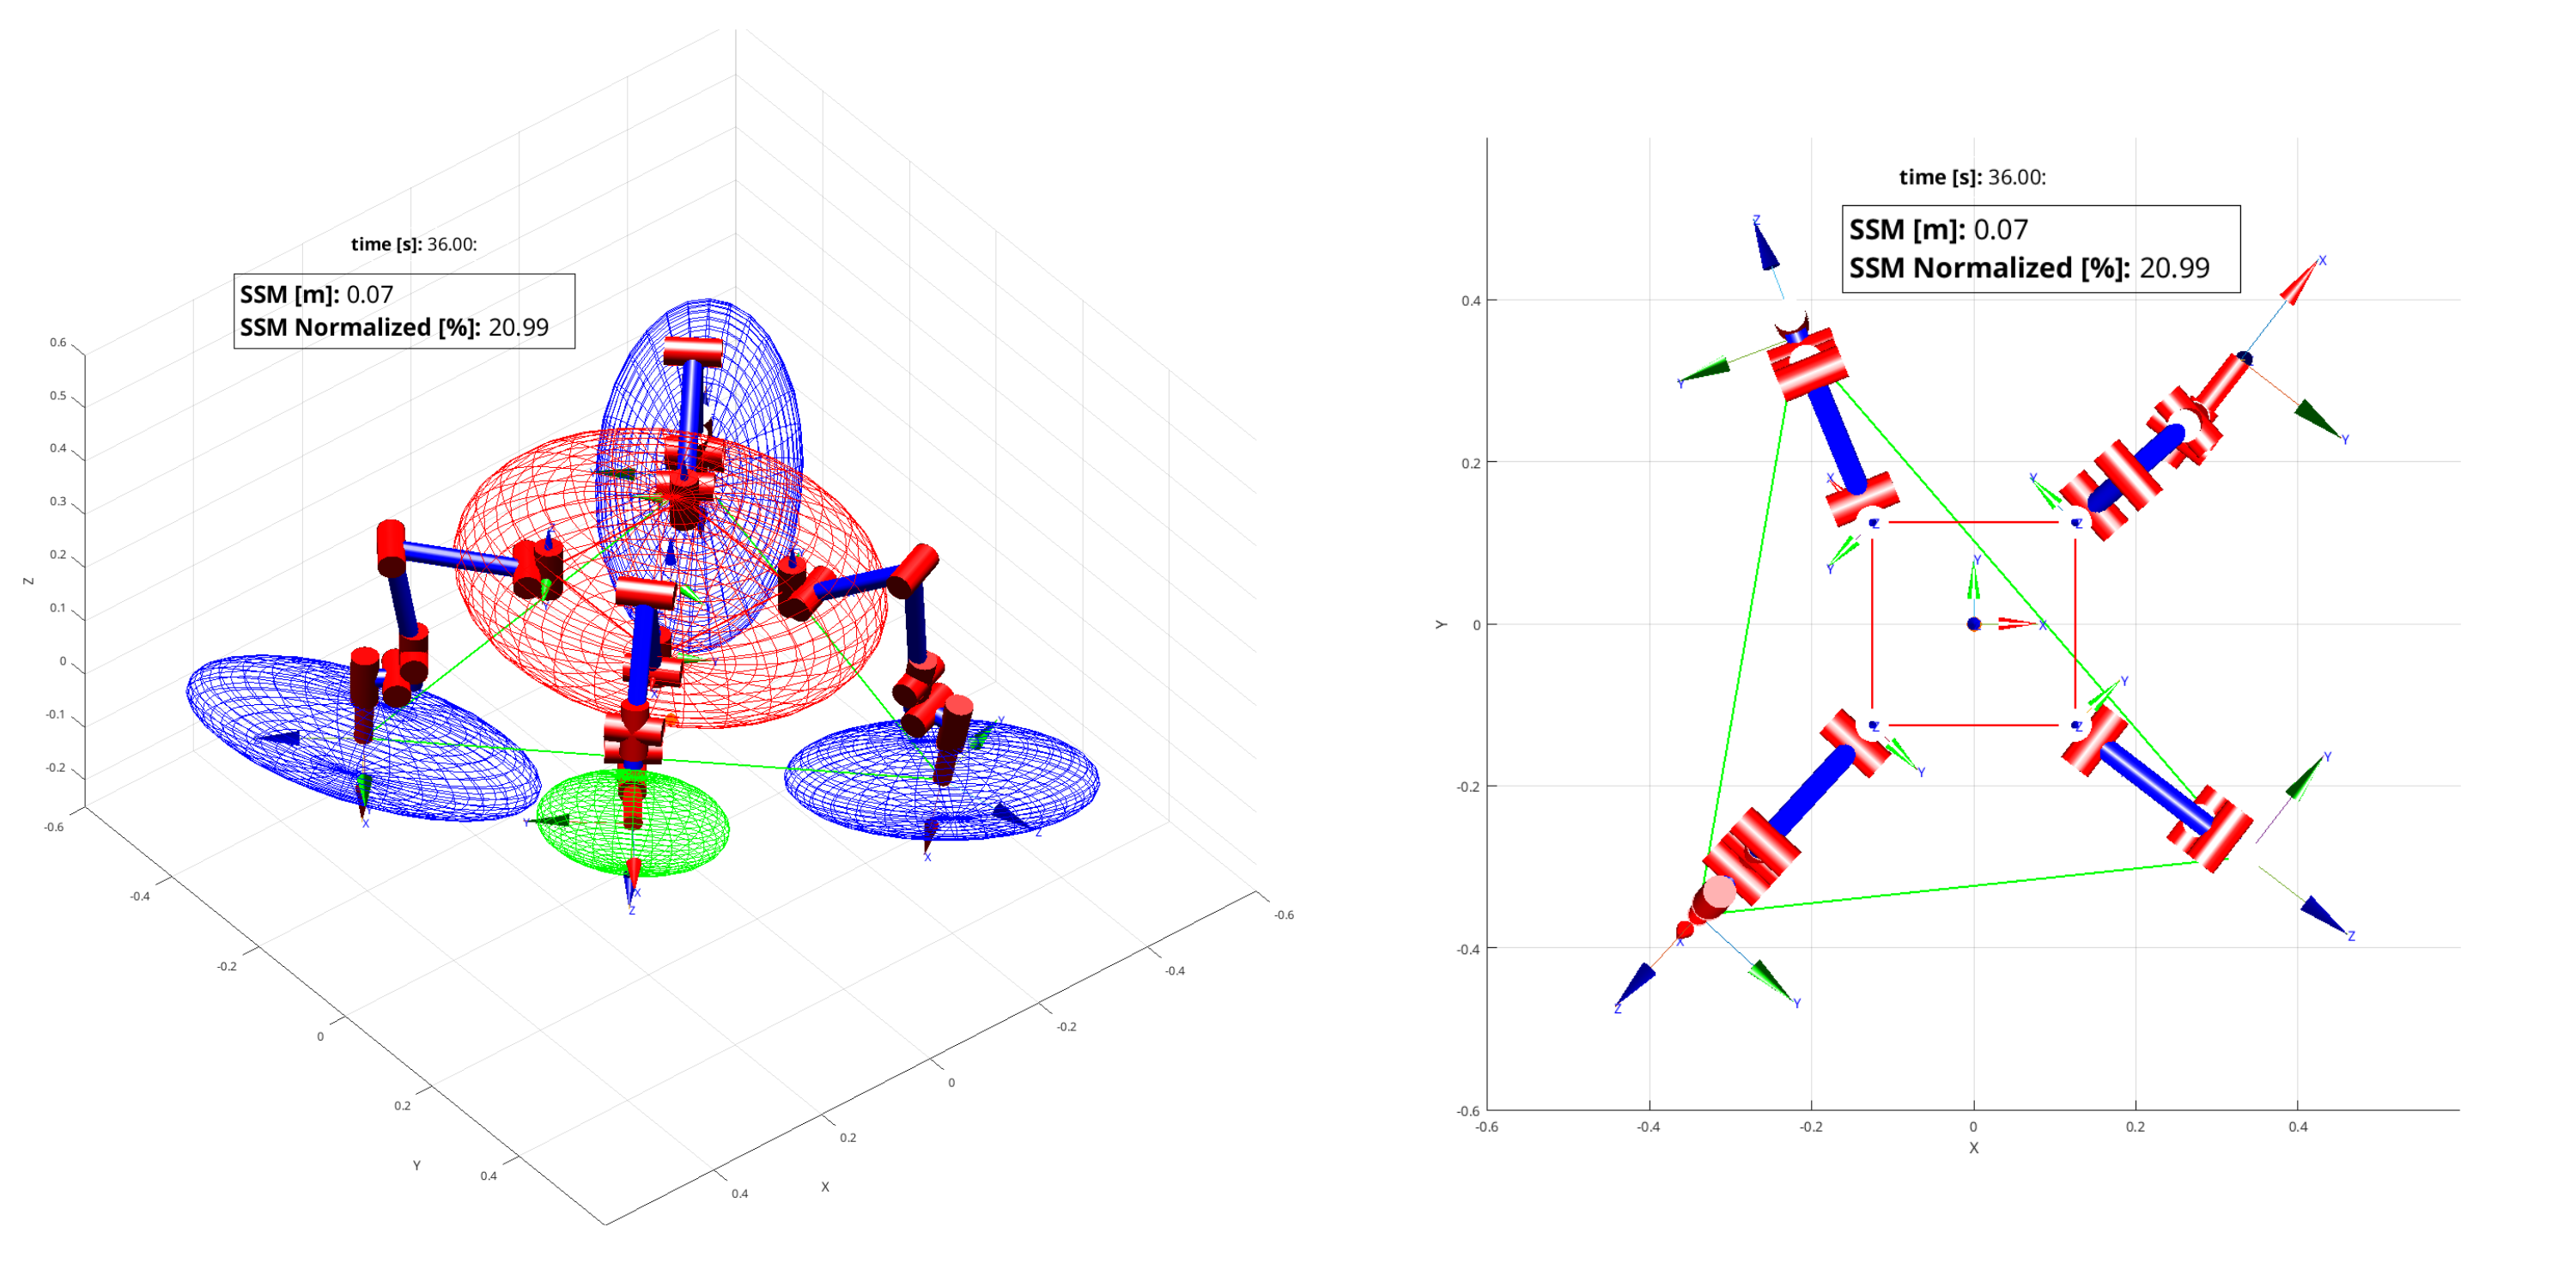
\includegraphics[width=0.55\textwidth]{Images/img_ch8/step3_exp.png}} 
    \subfloat[LF GRIEEL transformed (t=76 s)\label{fig:step4}]{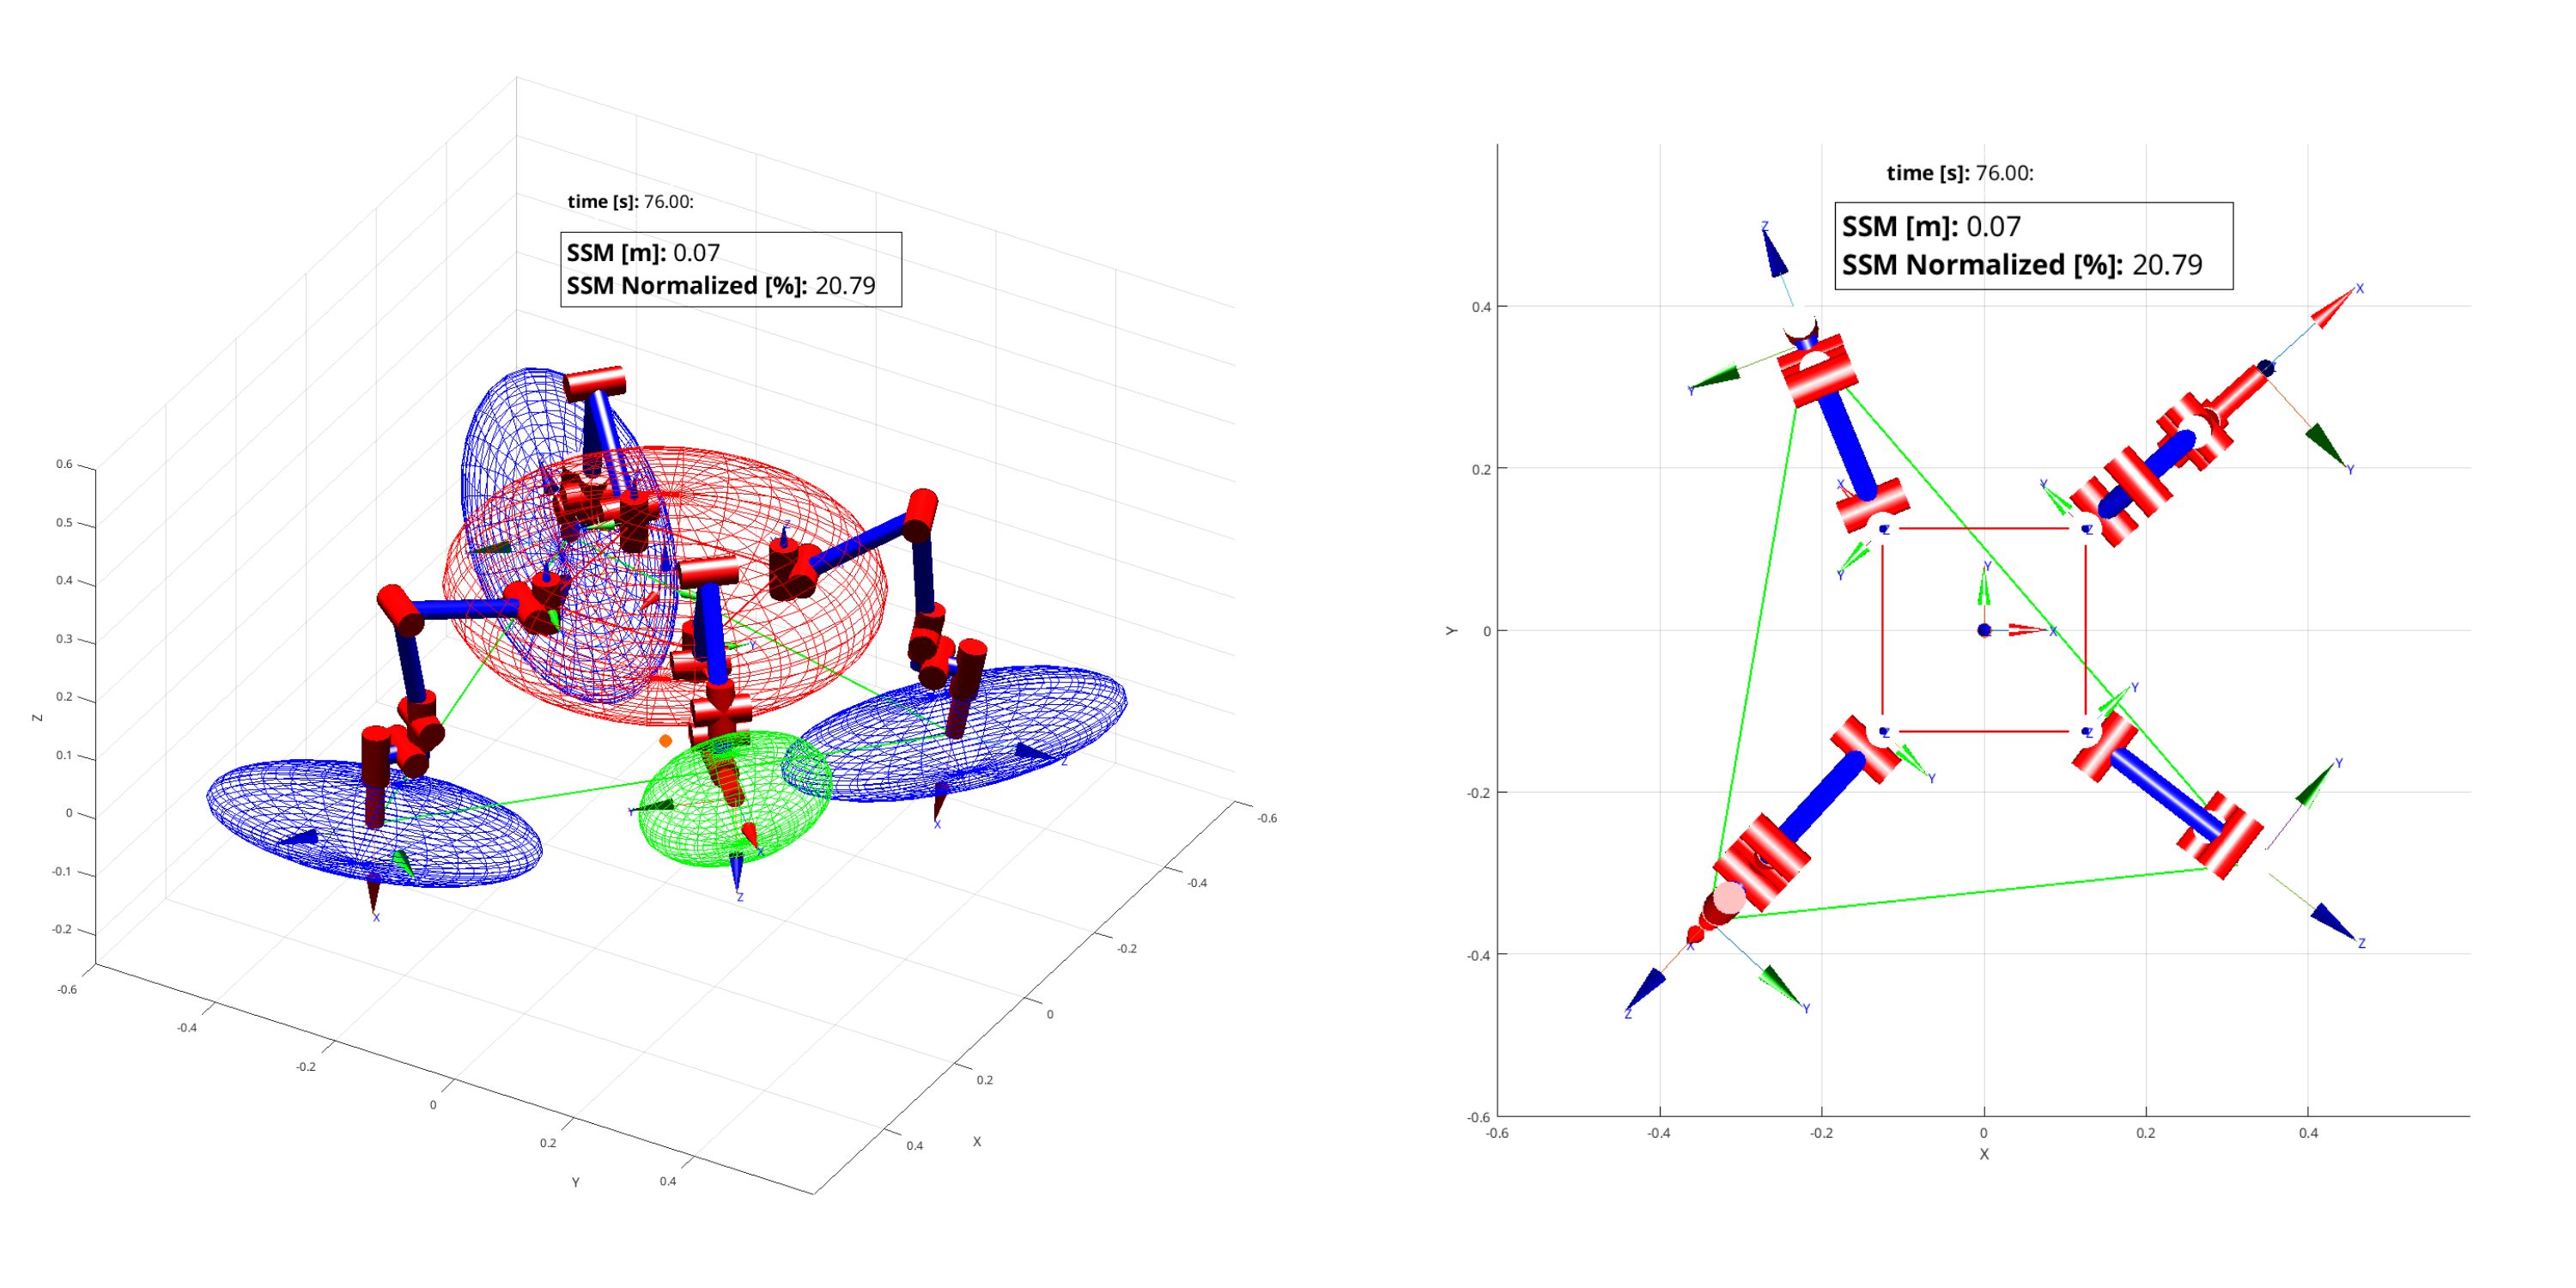
\includegraphics[width=0.55\textwidth]{Images/img_ch8/step4_exp.png}}\\ 
    
    \caption[Manipulability Ellipsoid during LF G2W transformation]{Manipulability Ellipsoid during LF G2W transformation}
    \label{fig:LF_manipulability}
\end{figure}

\begin{figure}[H]
    \centering
    \subfloat[LF Limb down (t=80 s)\label{fig:step5}]{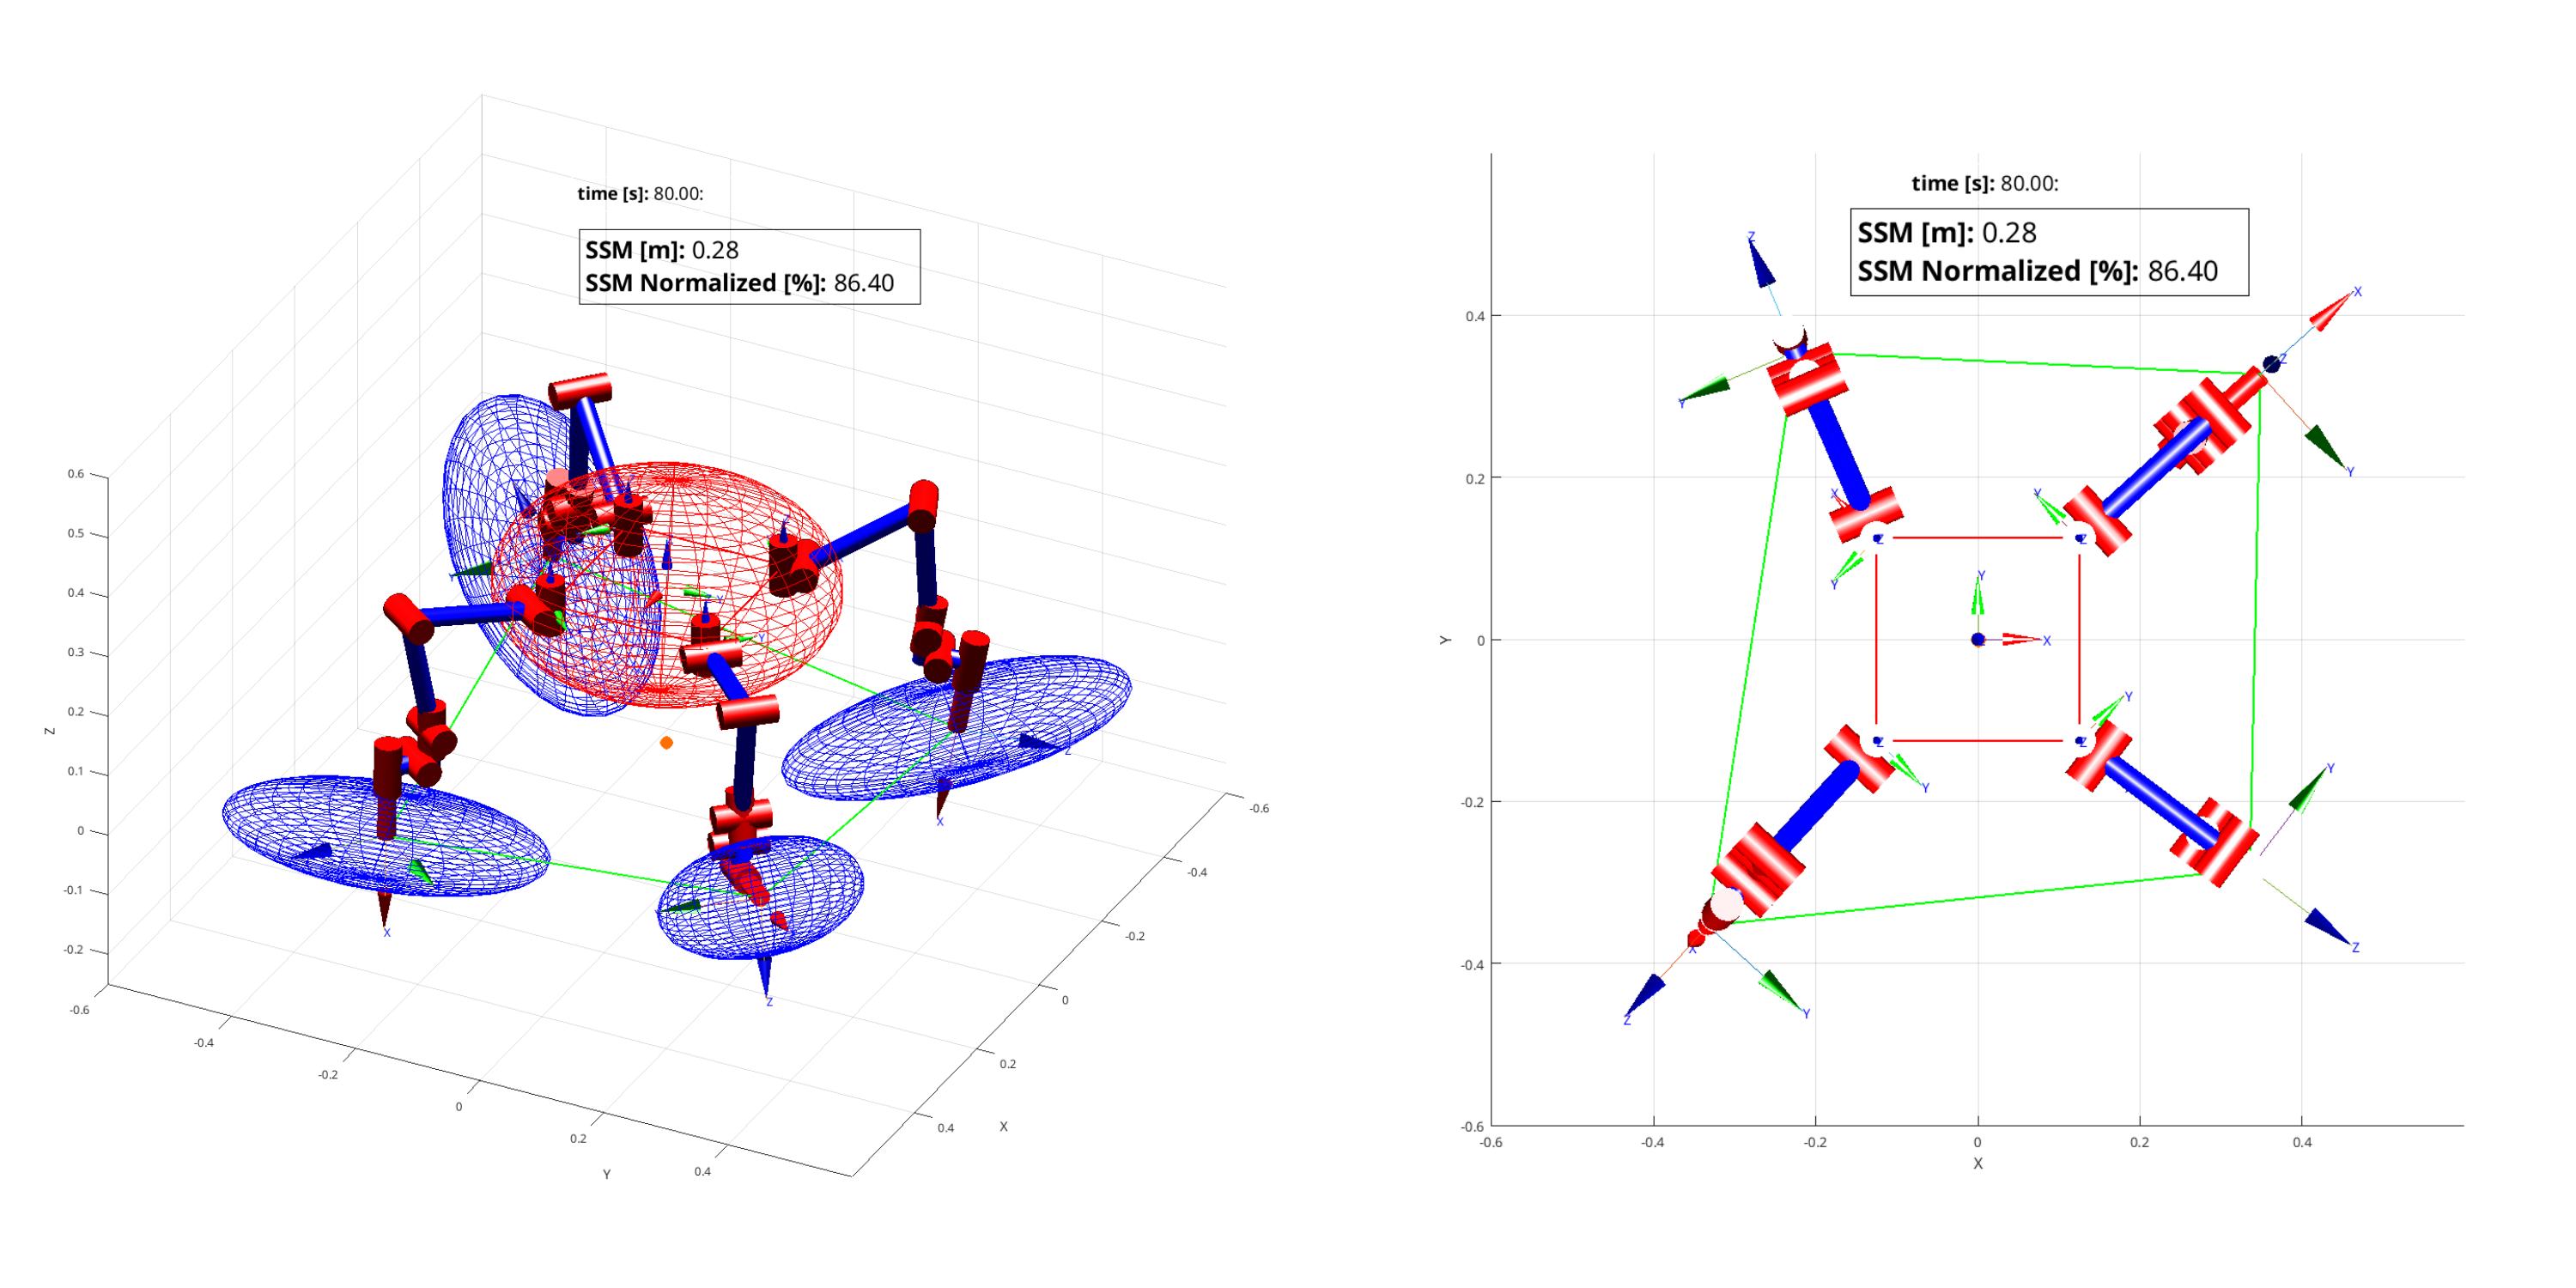
\includegraphics[width=0.55\textwidth]{Images/img_ch8/step5_exp.png}} 
    \subfloat[Base motion (t=84 s)\label{fig:step6}]{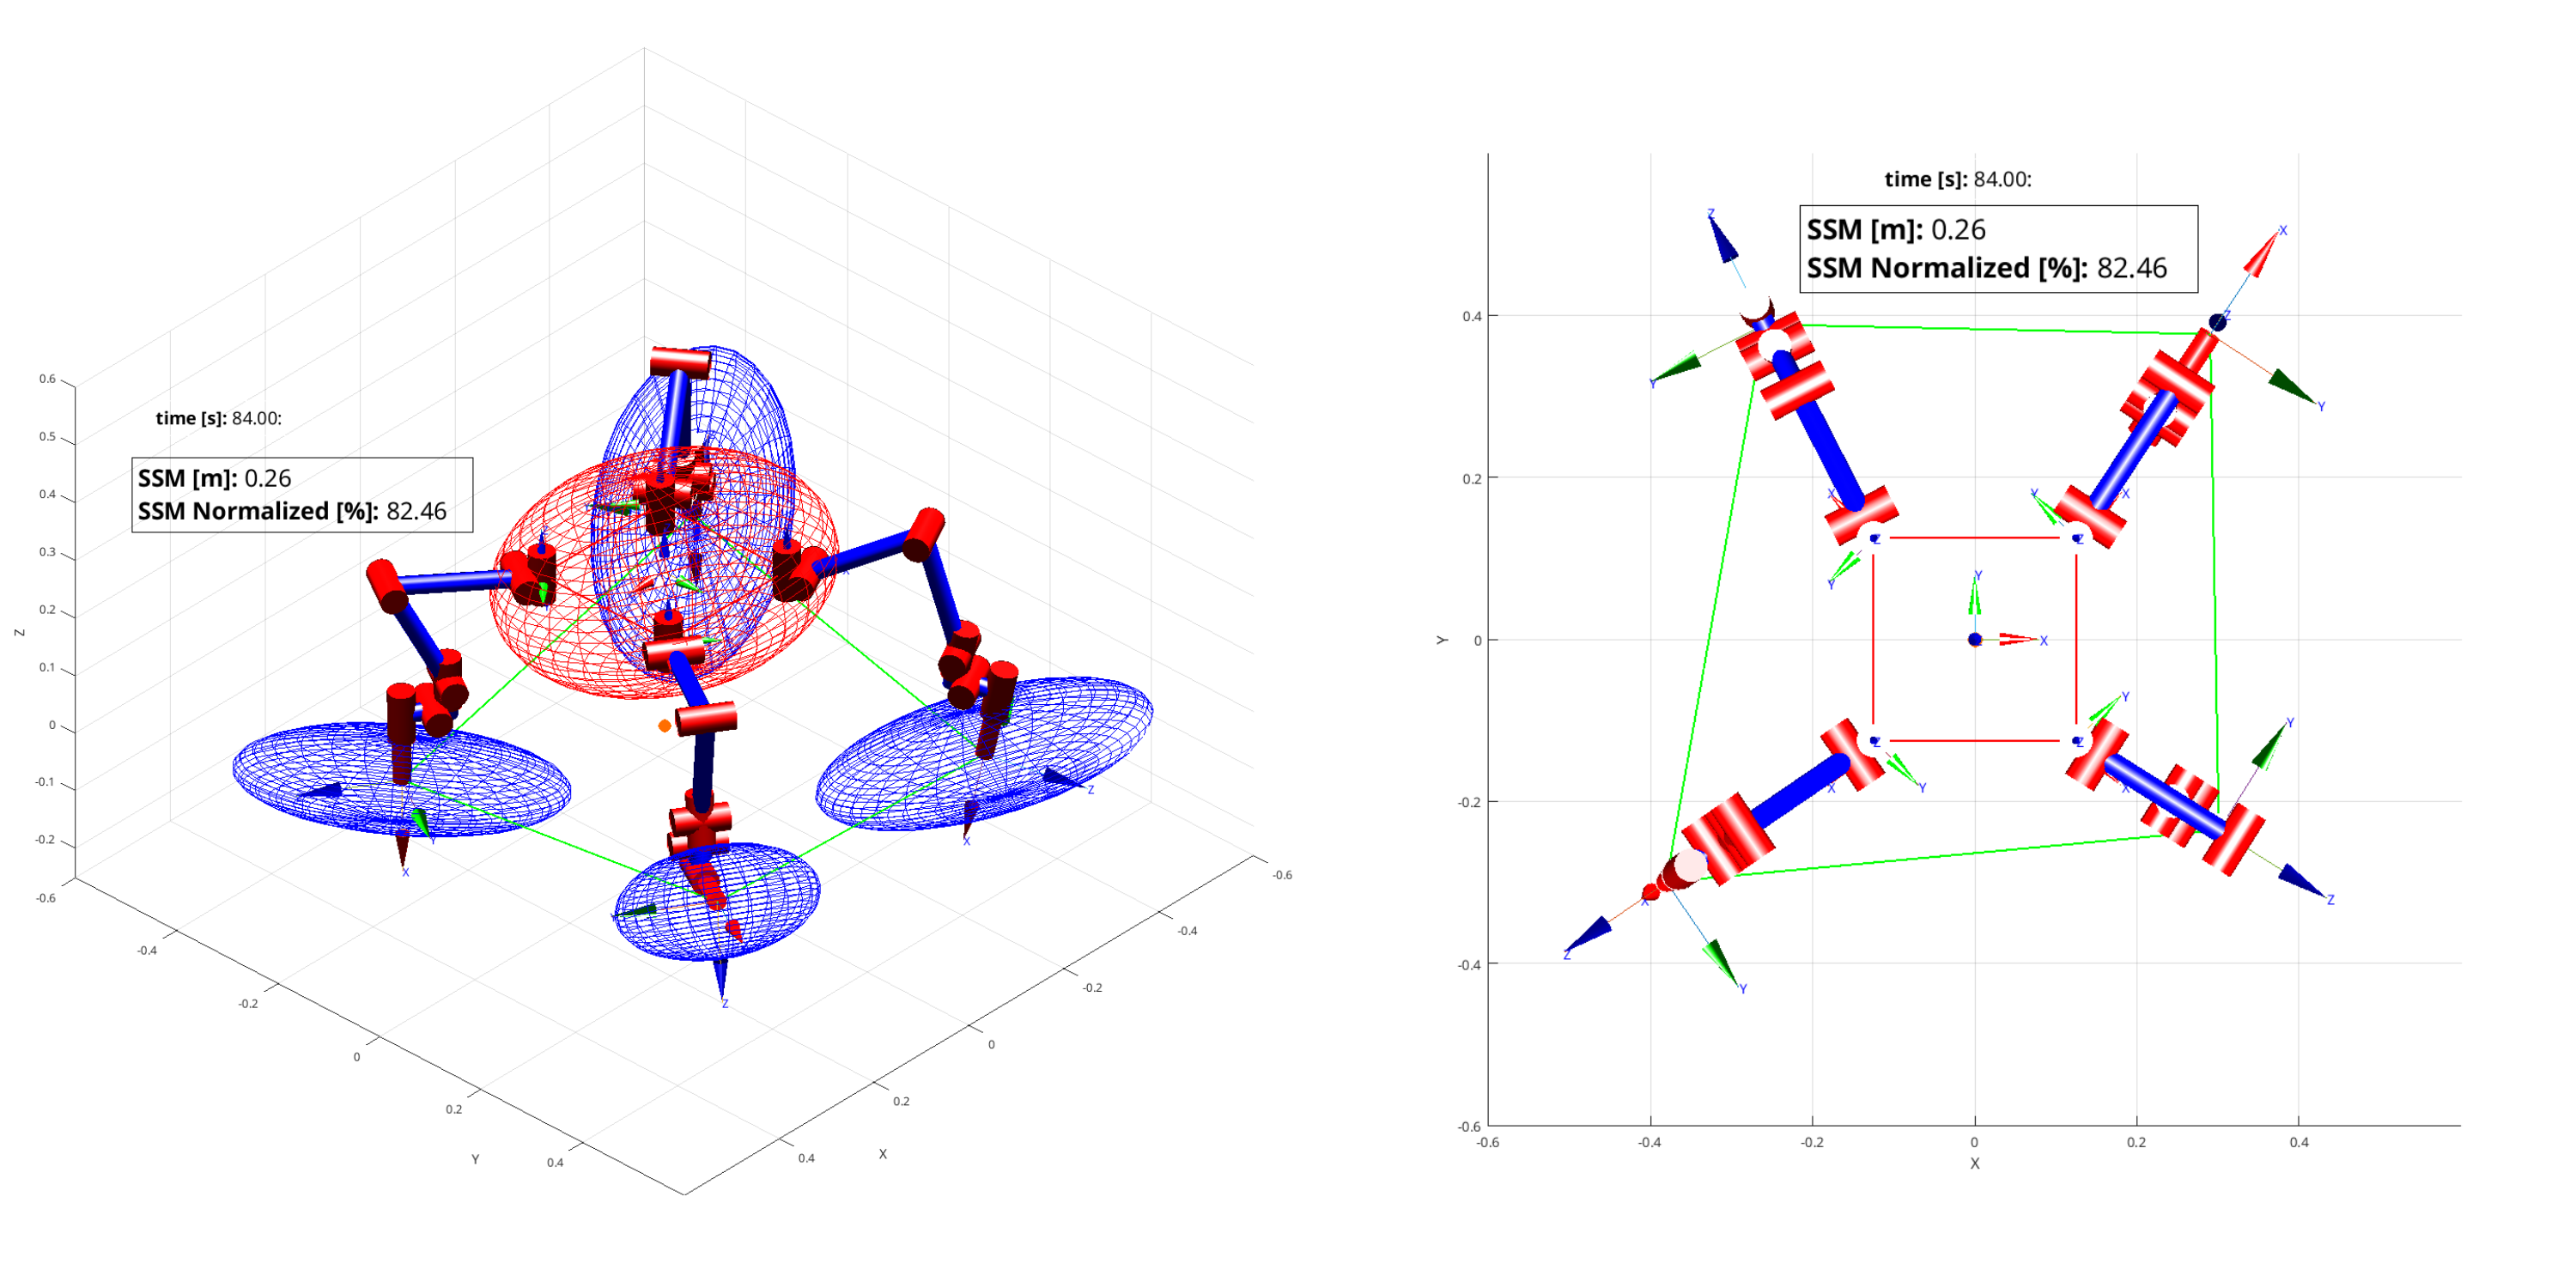
\includegraphics[width=0.55\textwidth]{Images/img_ch8/step6_exp.png}}\\ 

    \subfloat[Base motion (t=136 s)\label{fig:step7}]{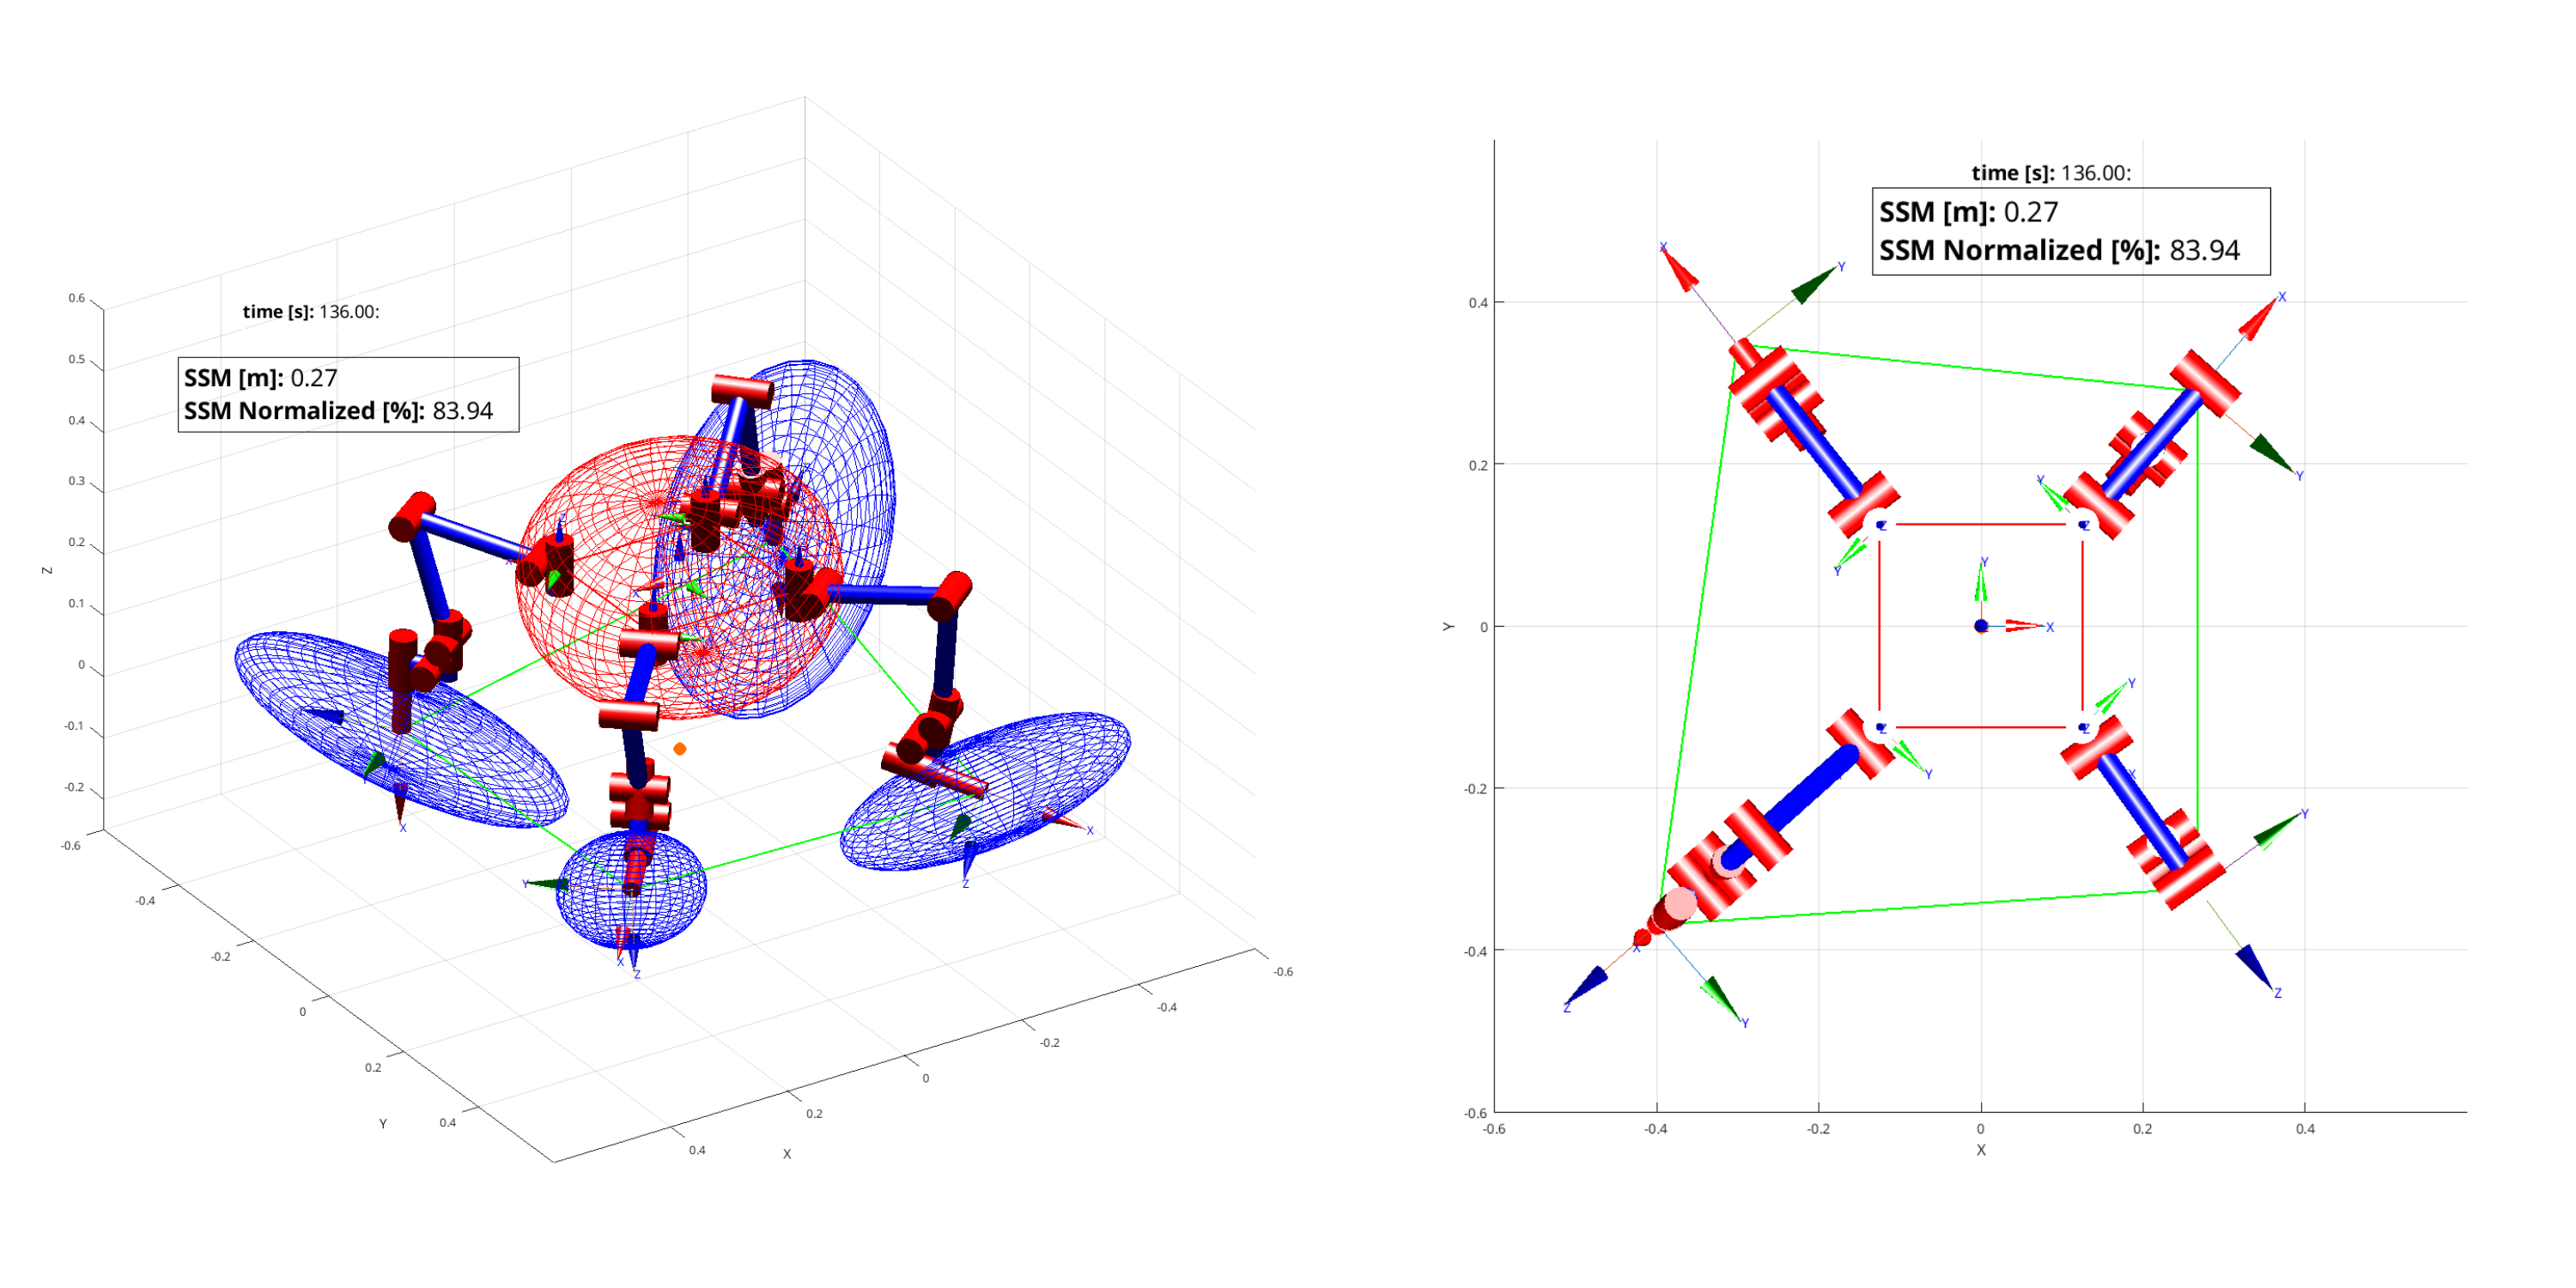
\includegraphics[width=0.55\textwidth]{Images/img_ch8/step7_exp.png}} 
    \subfloat[RH Limb down (t=192 s)\label{fig:step8}]{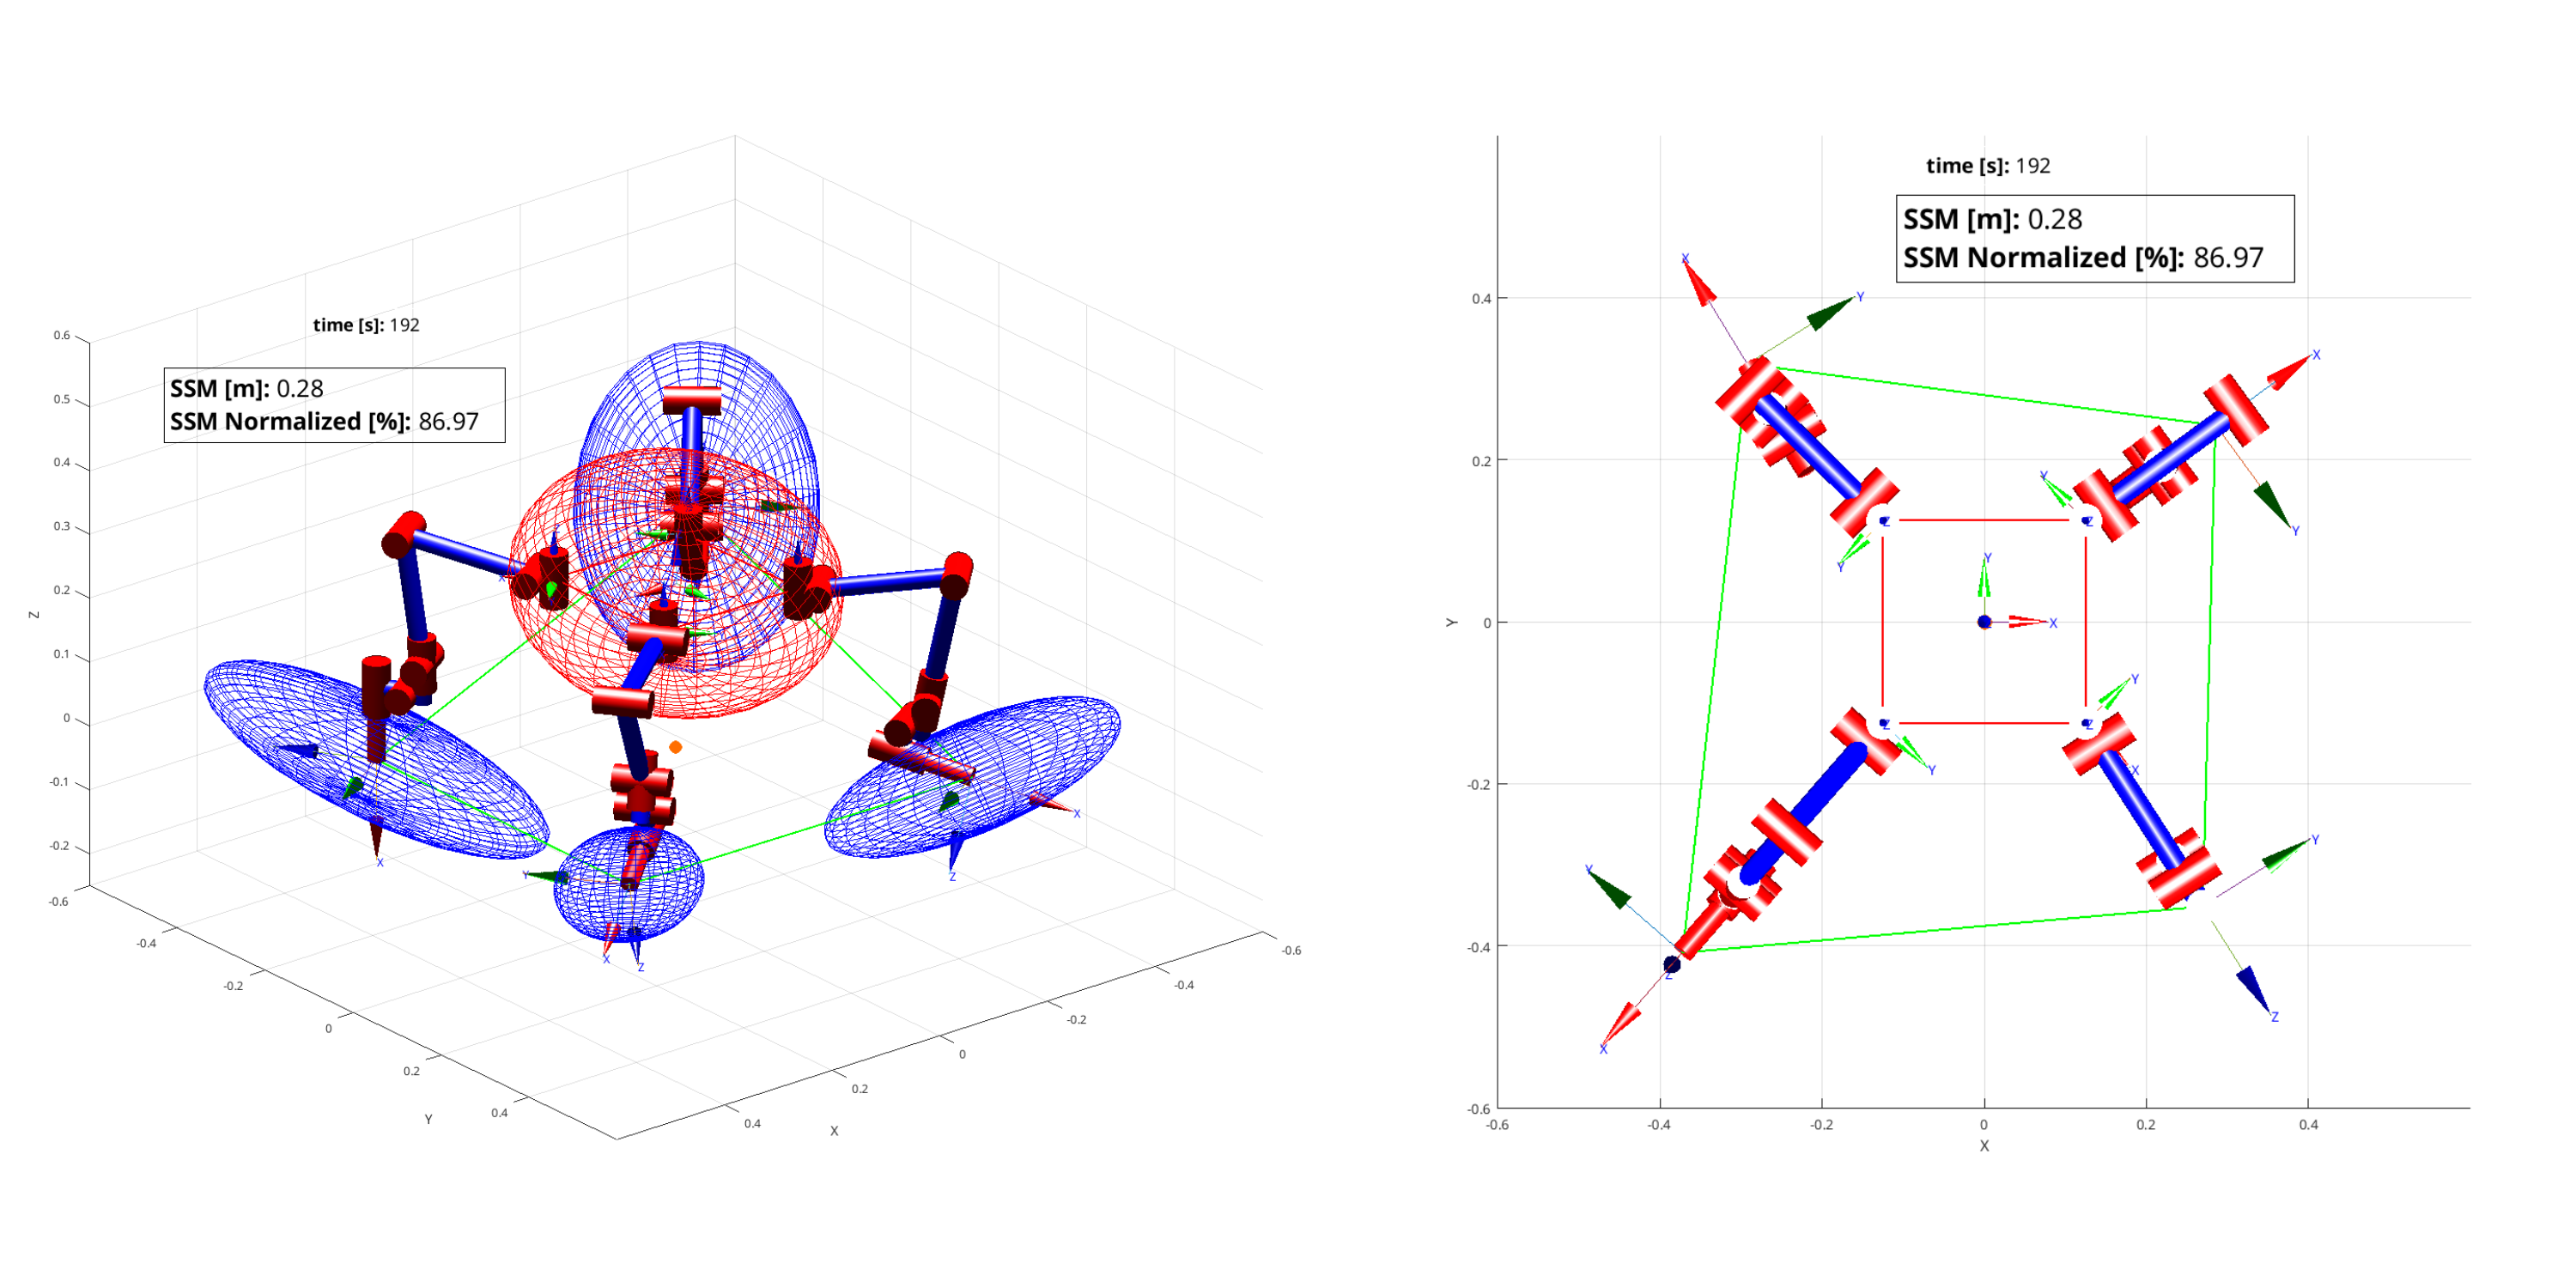
\includegraphics[width=0.55\textwidth]{Images/img_ch8/step8_exp.png}}\\ 
    
    \caption[Manipulability Ellipsoid during LH and RH G2W transformation]{Manipulability Ellipsoid during LH and RH G2W transformation}
    \label{fig:LH_RH_manipulability}
\end{figure}

\newpage
\section{Simulation Results, Gazebo Harmonic}
\label{sec:sim_result_harmonic}

Using a more reliable simulation environment, additional tests have been conducted. 
This section reports the results of walking-to-driving (G2W) locomotion transition, driving motion with four or three support wheels, and driving-to-walking mode transformation (W2G). In particular, joint state tracking, torque control actions, and static stability margins are reported here. The dexterity analysis is not shown for conciseness because its results are similar to the experimental one and to the dexterity analysis on the algorithm conducted in Chapter \ref{ch:chapter_five}.  

%% --- GRIPPER TO WHEEL ---
\subsection{Gripper to Wheel (G2W)}
\label{sec:gz_harmonic_G2W}

Some steps of the G2W transformation in the simulator are shown in Fig.\ref{fig:G2W_harmonic}. The joint state tracking for each limb is represented in Figs.\ref{fig:G2W_LF_harmonic_joint} - \ref{fig:G2W_RF_harmonic_joint}, while the control torque from the IJCs in Figs.\ref{fig:G2W_LF_harmonic_torque} - \ref{fig:G2W_RF_harmonic_torque}.
Finally, the stability margins during the motion sequence are reported in Fig.\ref{fig:G2W_SSM_harmonic}.

\begin{figure}[H]
    \centering
    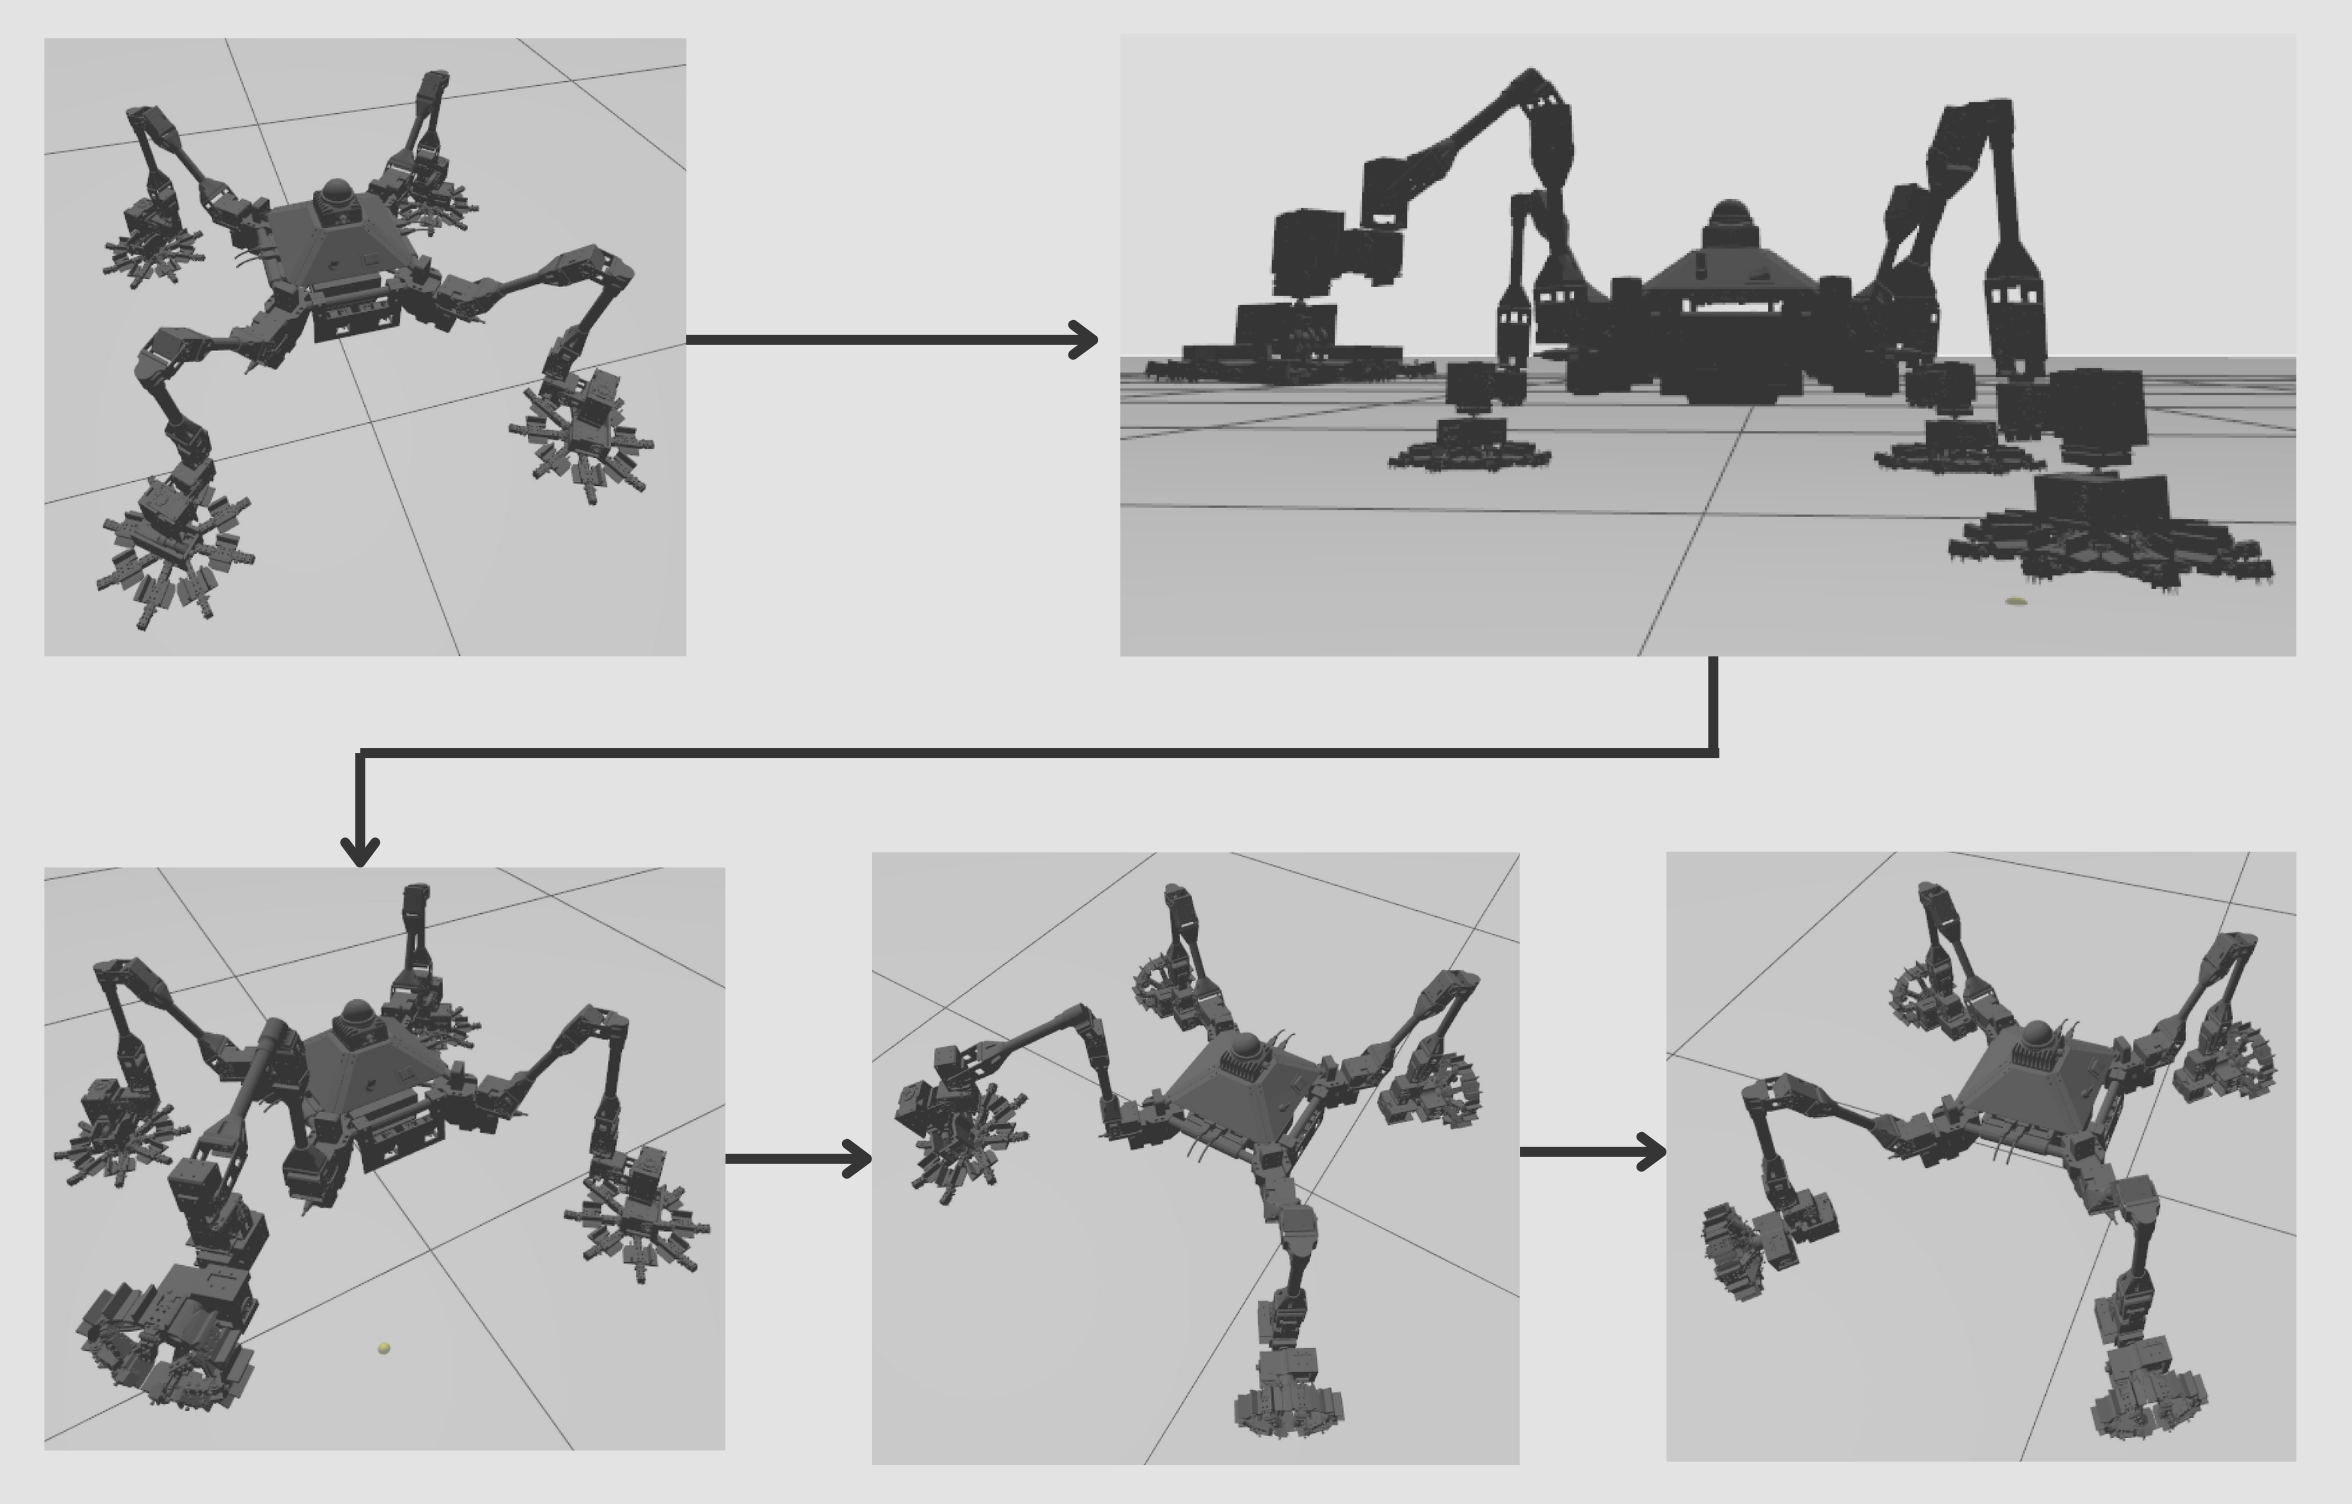
\includegraphics[width=0.9\textwidth]{Images/img_ch8/G2W_steps_sim.png}
    \caption{G2W Transition sequence in Gazebo Harmonic}
    \label{fig:G2W_harmonic}
\end{figure}

\begin{figure}[H]
    \centering
    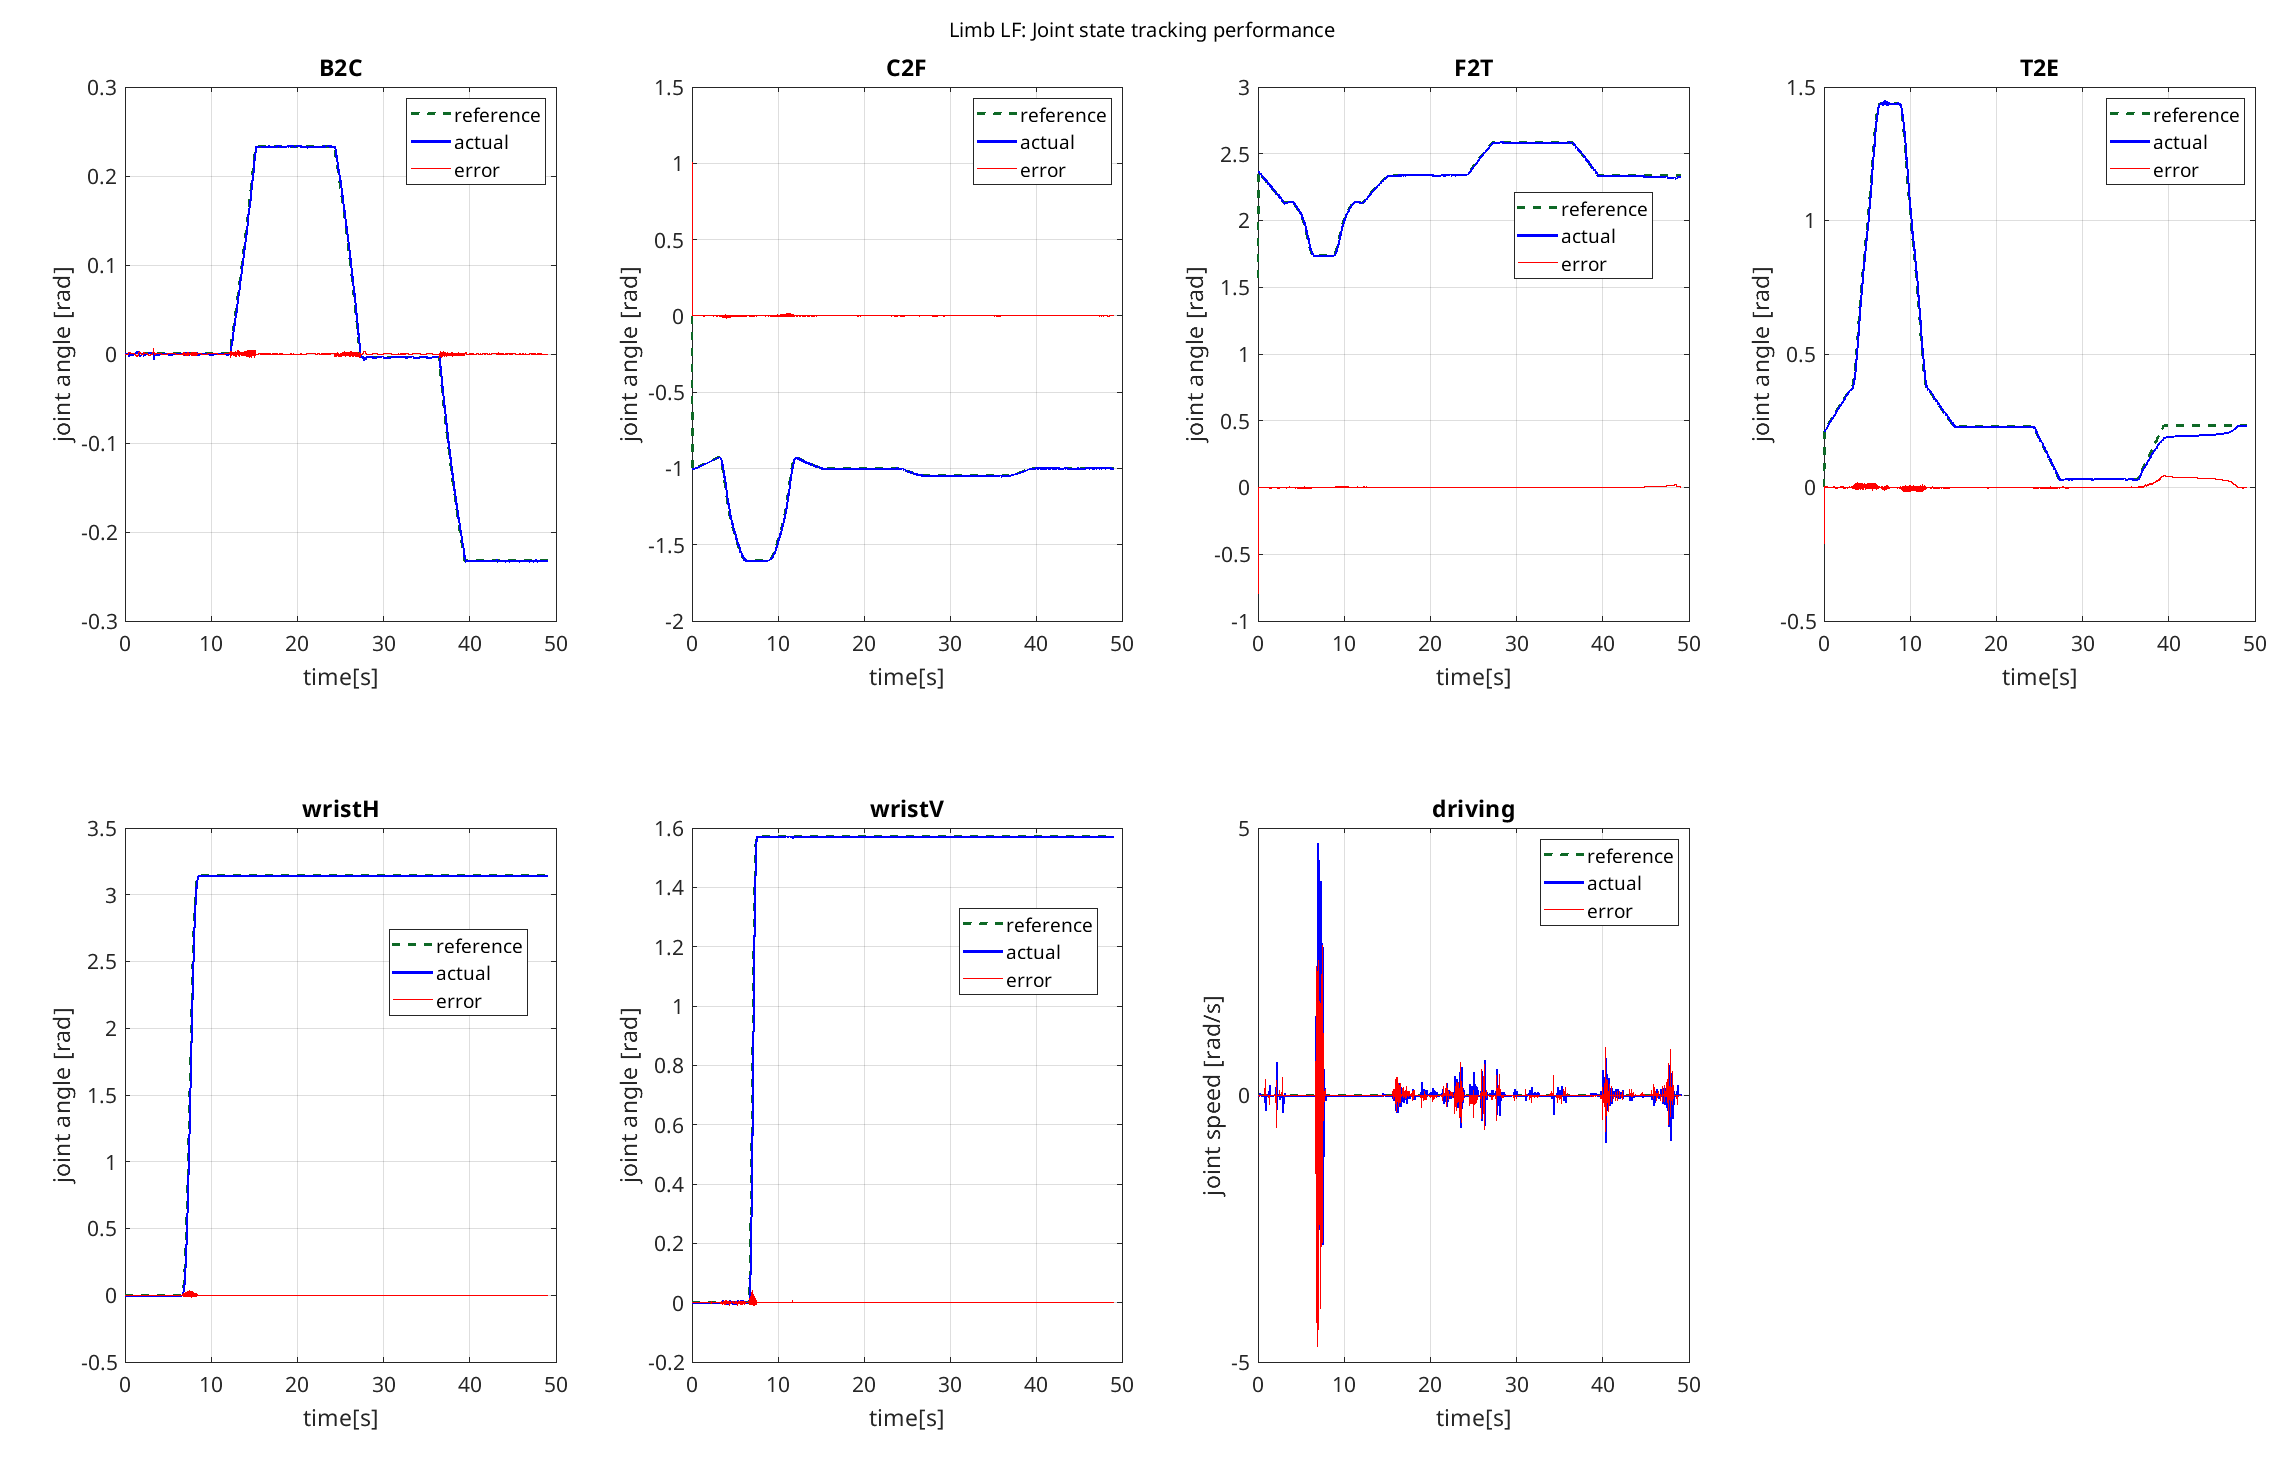
\includegraphics[width=1.0\textwidth]{Images/img_ch8/G2W_LF_joints.png}
    \caption{LF limb, Joint tracking during G2W}
    \label{fig:G2W_LF_harmonic_joint}
\end{figure}

\begin{figure}[H]
    \centering
    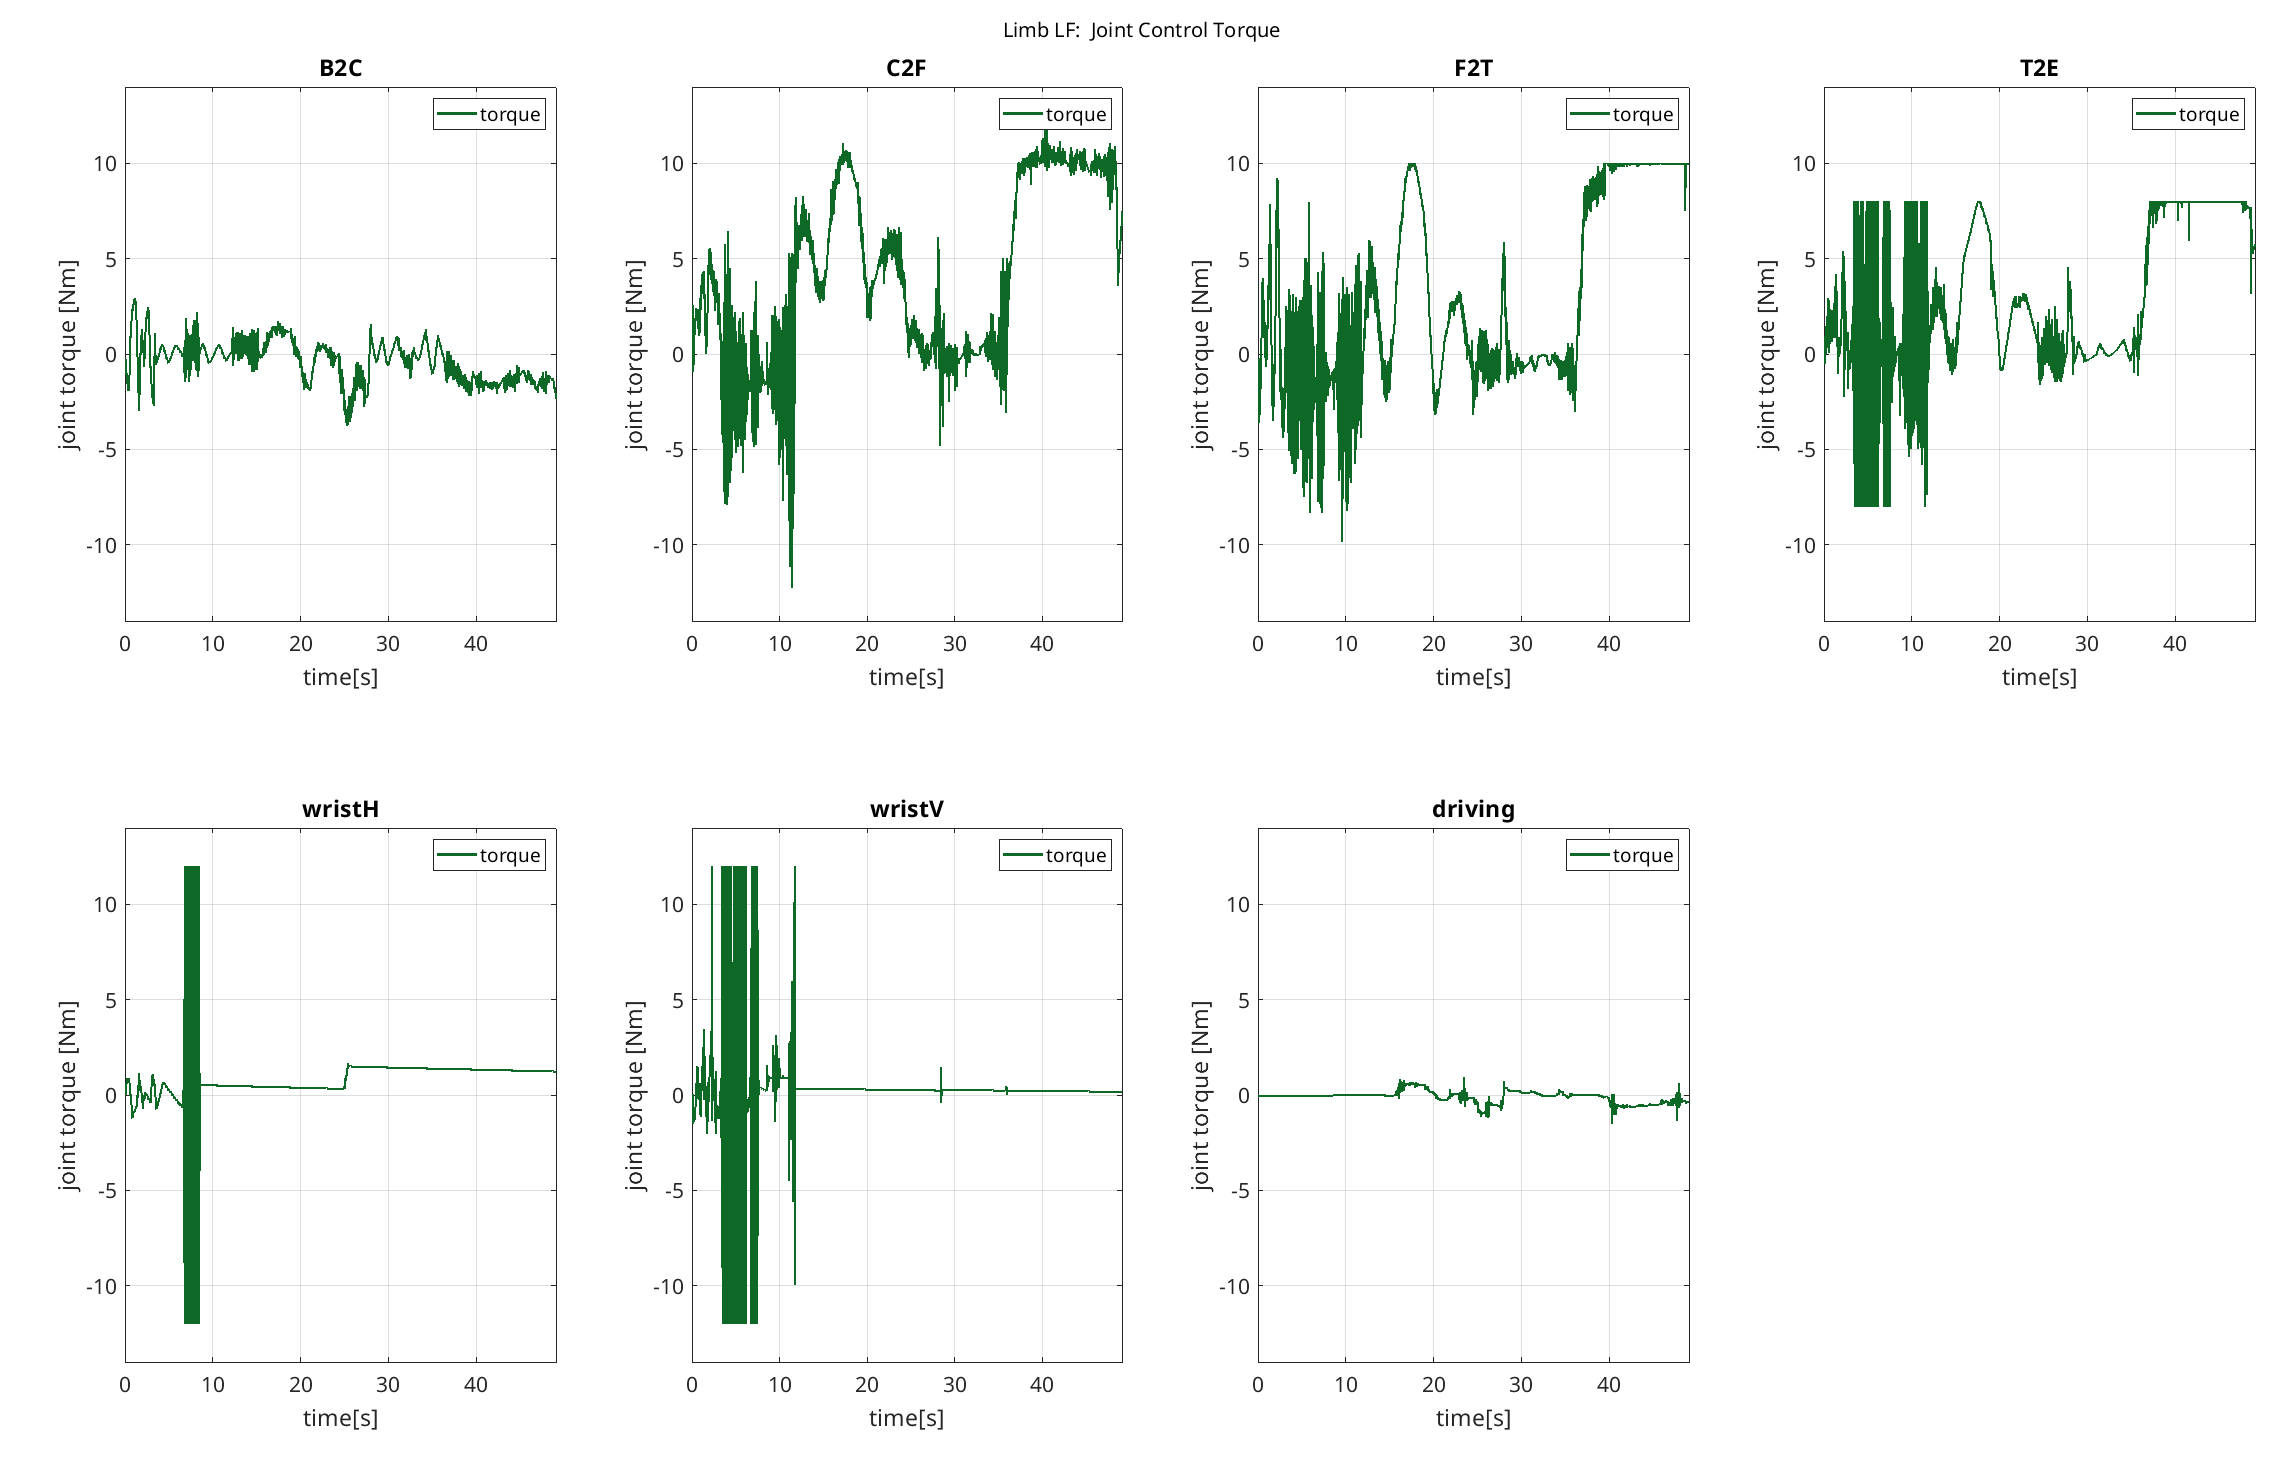
\includegraphics[width=1.0\textwidth]{Images/img_ch8/G2W_LF_torque.png}
    \caption{LF limb, Joint torques during G2W}
    \label{fig:G2W_LF_harmonic_torque}
\end{figure}

\begin{figure}[H]
    \centering
    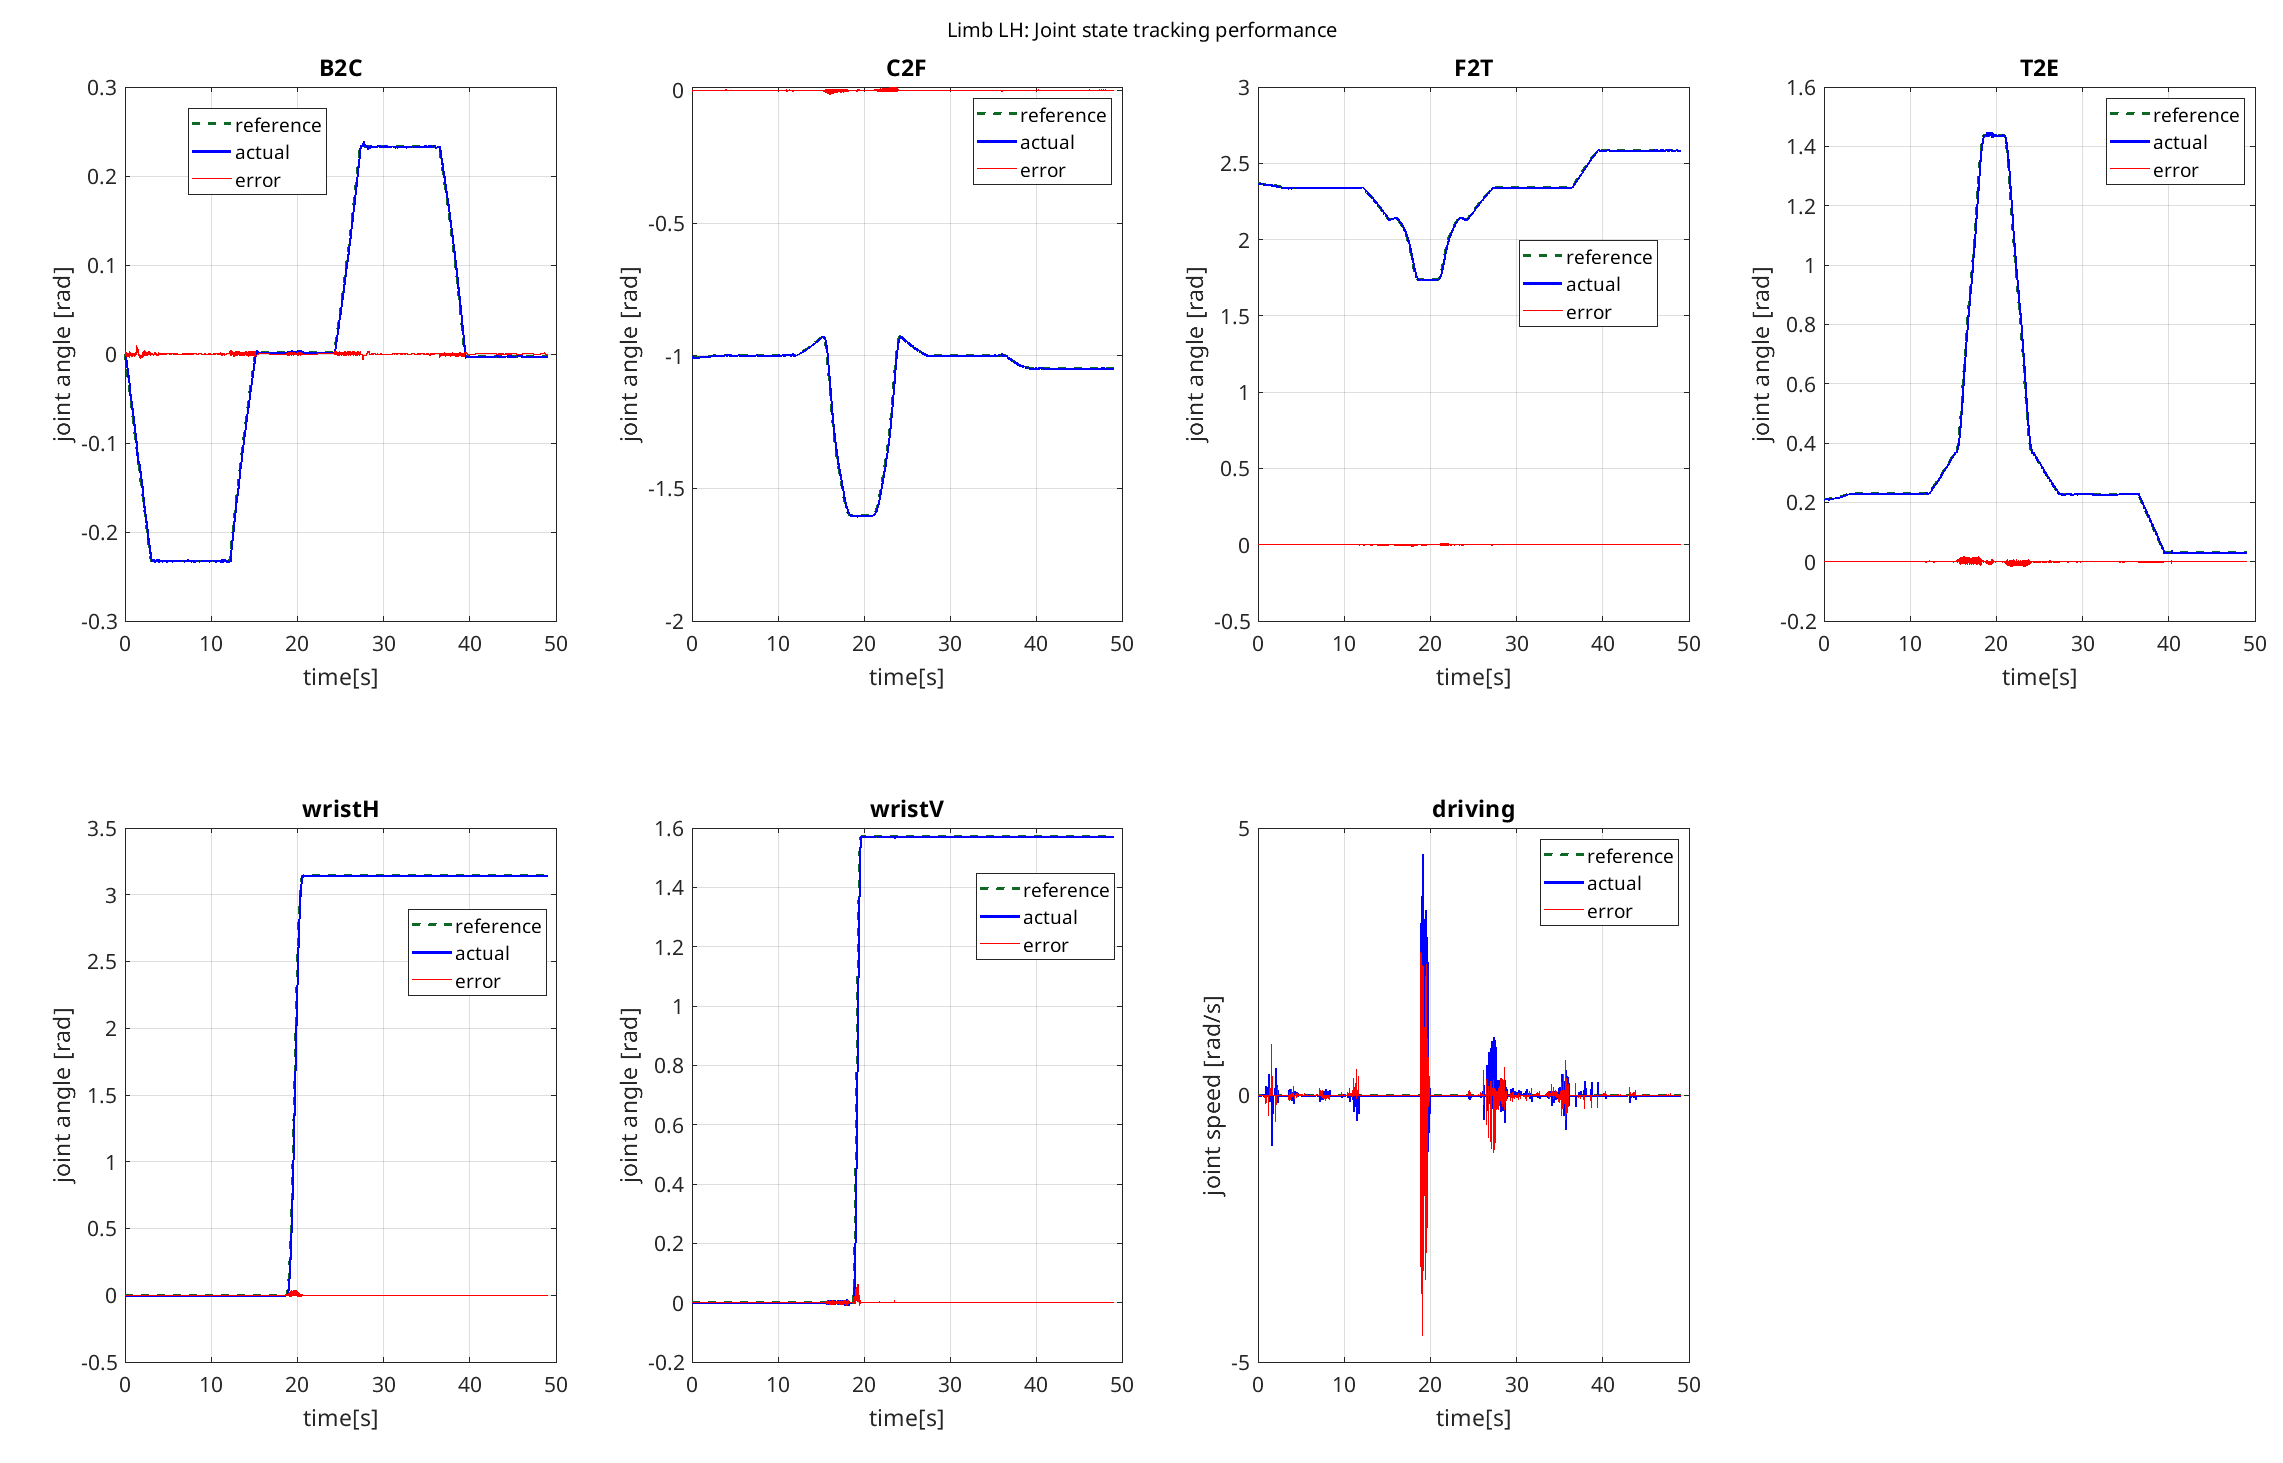
\includegraphics[width=1.0\textwidth]{Images/img_ch8/G2W_LH_joints.png}
    \caption{LH limb, Joint tracking during G2W}
    \label{fig:G2W_LH_harmonic_joint}
\end{figure}

\begin{figure}[H]
    \centering
    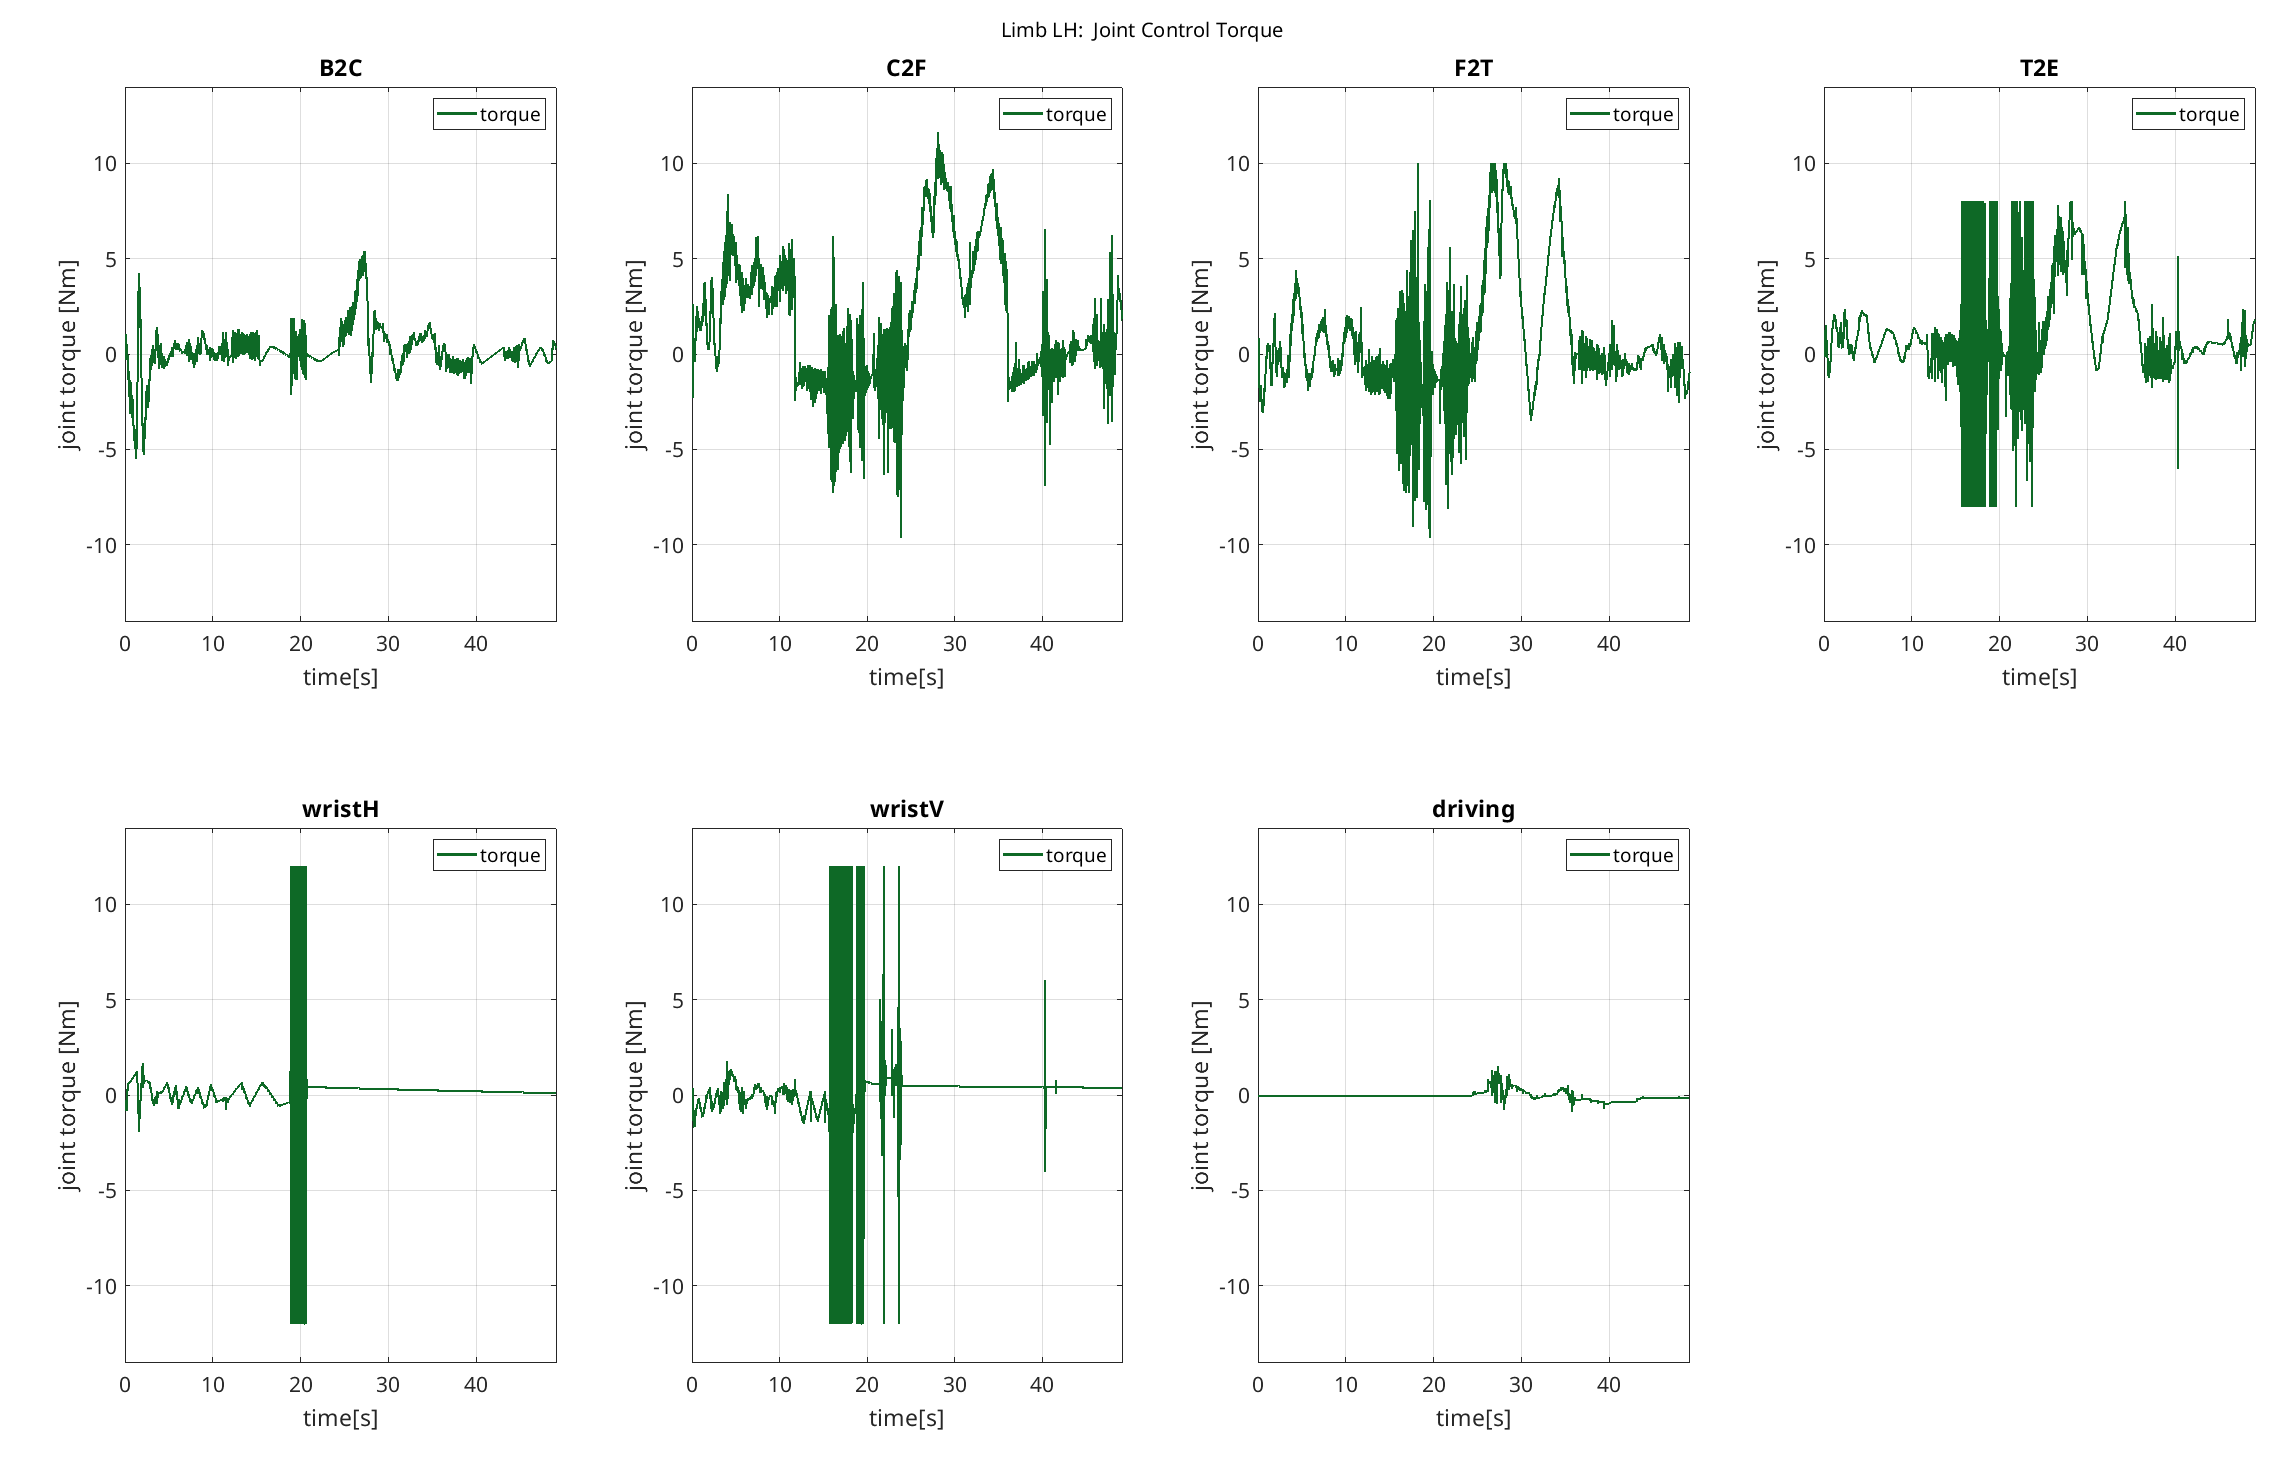
\includegraphics[width=1.0\textwidth]{Images/img_ch8/G2W_LH_torque.png}
    \caption{LH limb, Joint torques during G2W}
    \label{fig:G2W_LF_harmonic_torque}
\end{figure}
\begin{figure}[H]
    \centering
    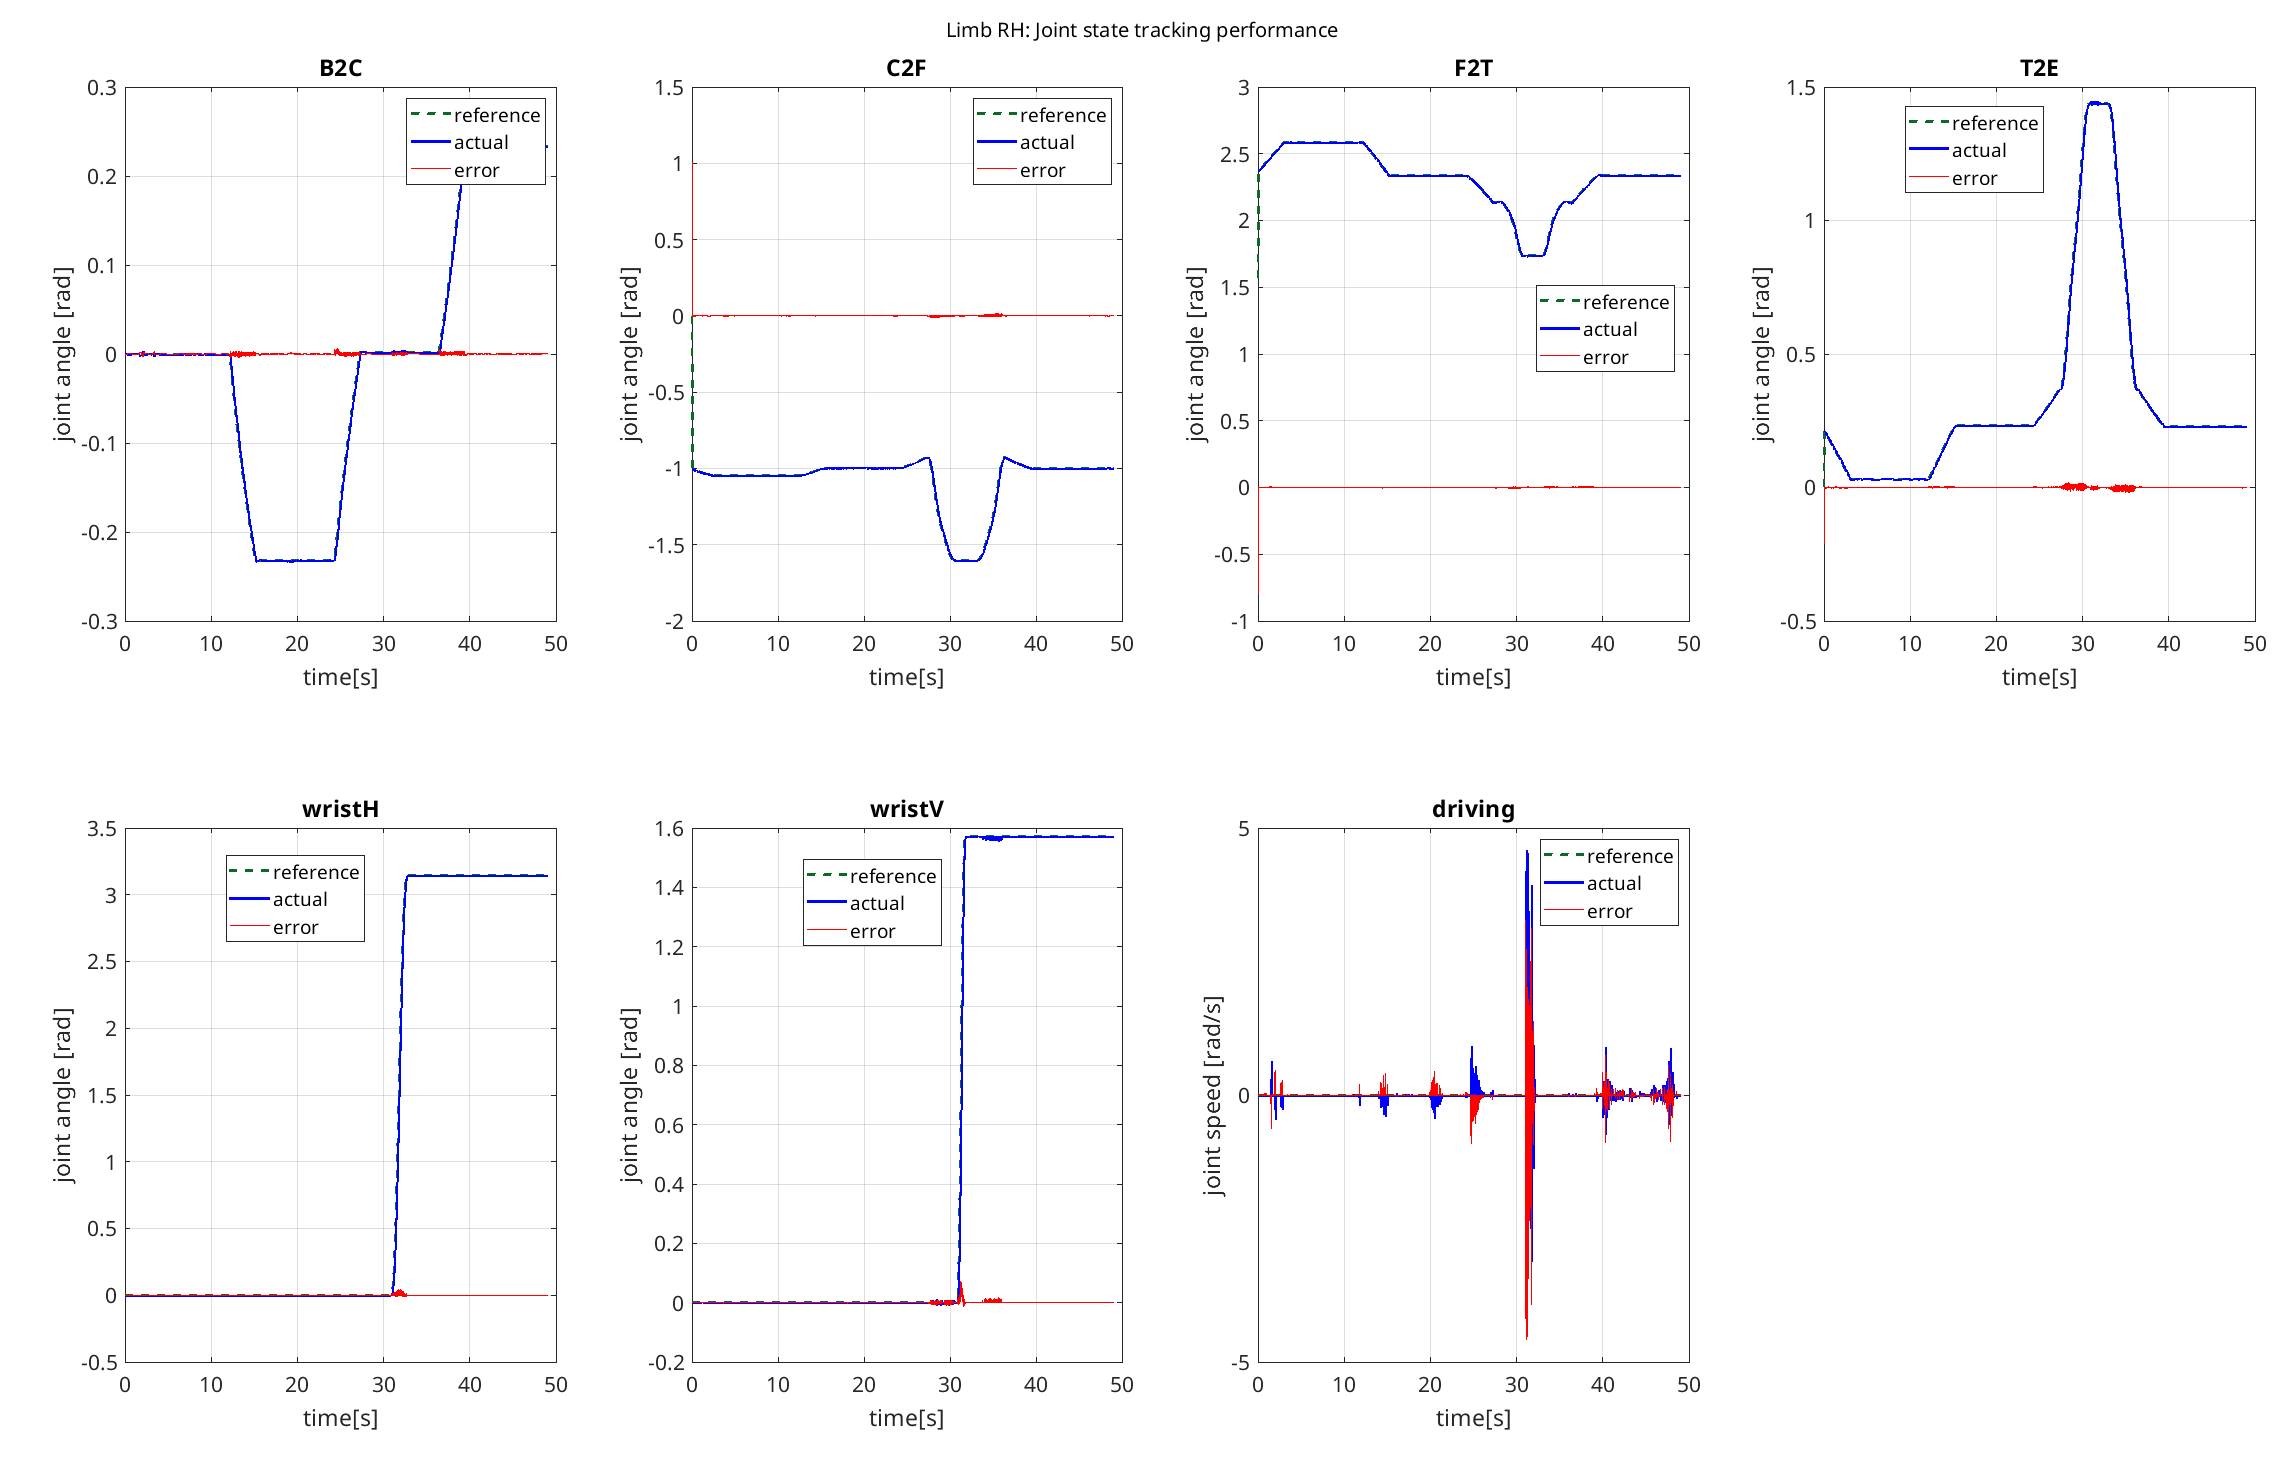
\includegraphics[width=1.0\textwidth]{Images/img_ch8/G2W_RH_joints.png}
    \caption{RH limb, Joint tracking during G2W}
    \label{fig:G2W_RH_harmonic_joint}
\end{figure}

\begin{figure}[H]
    \centering
    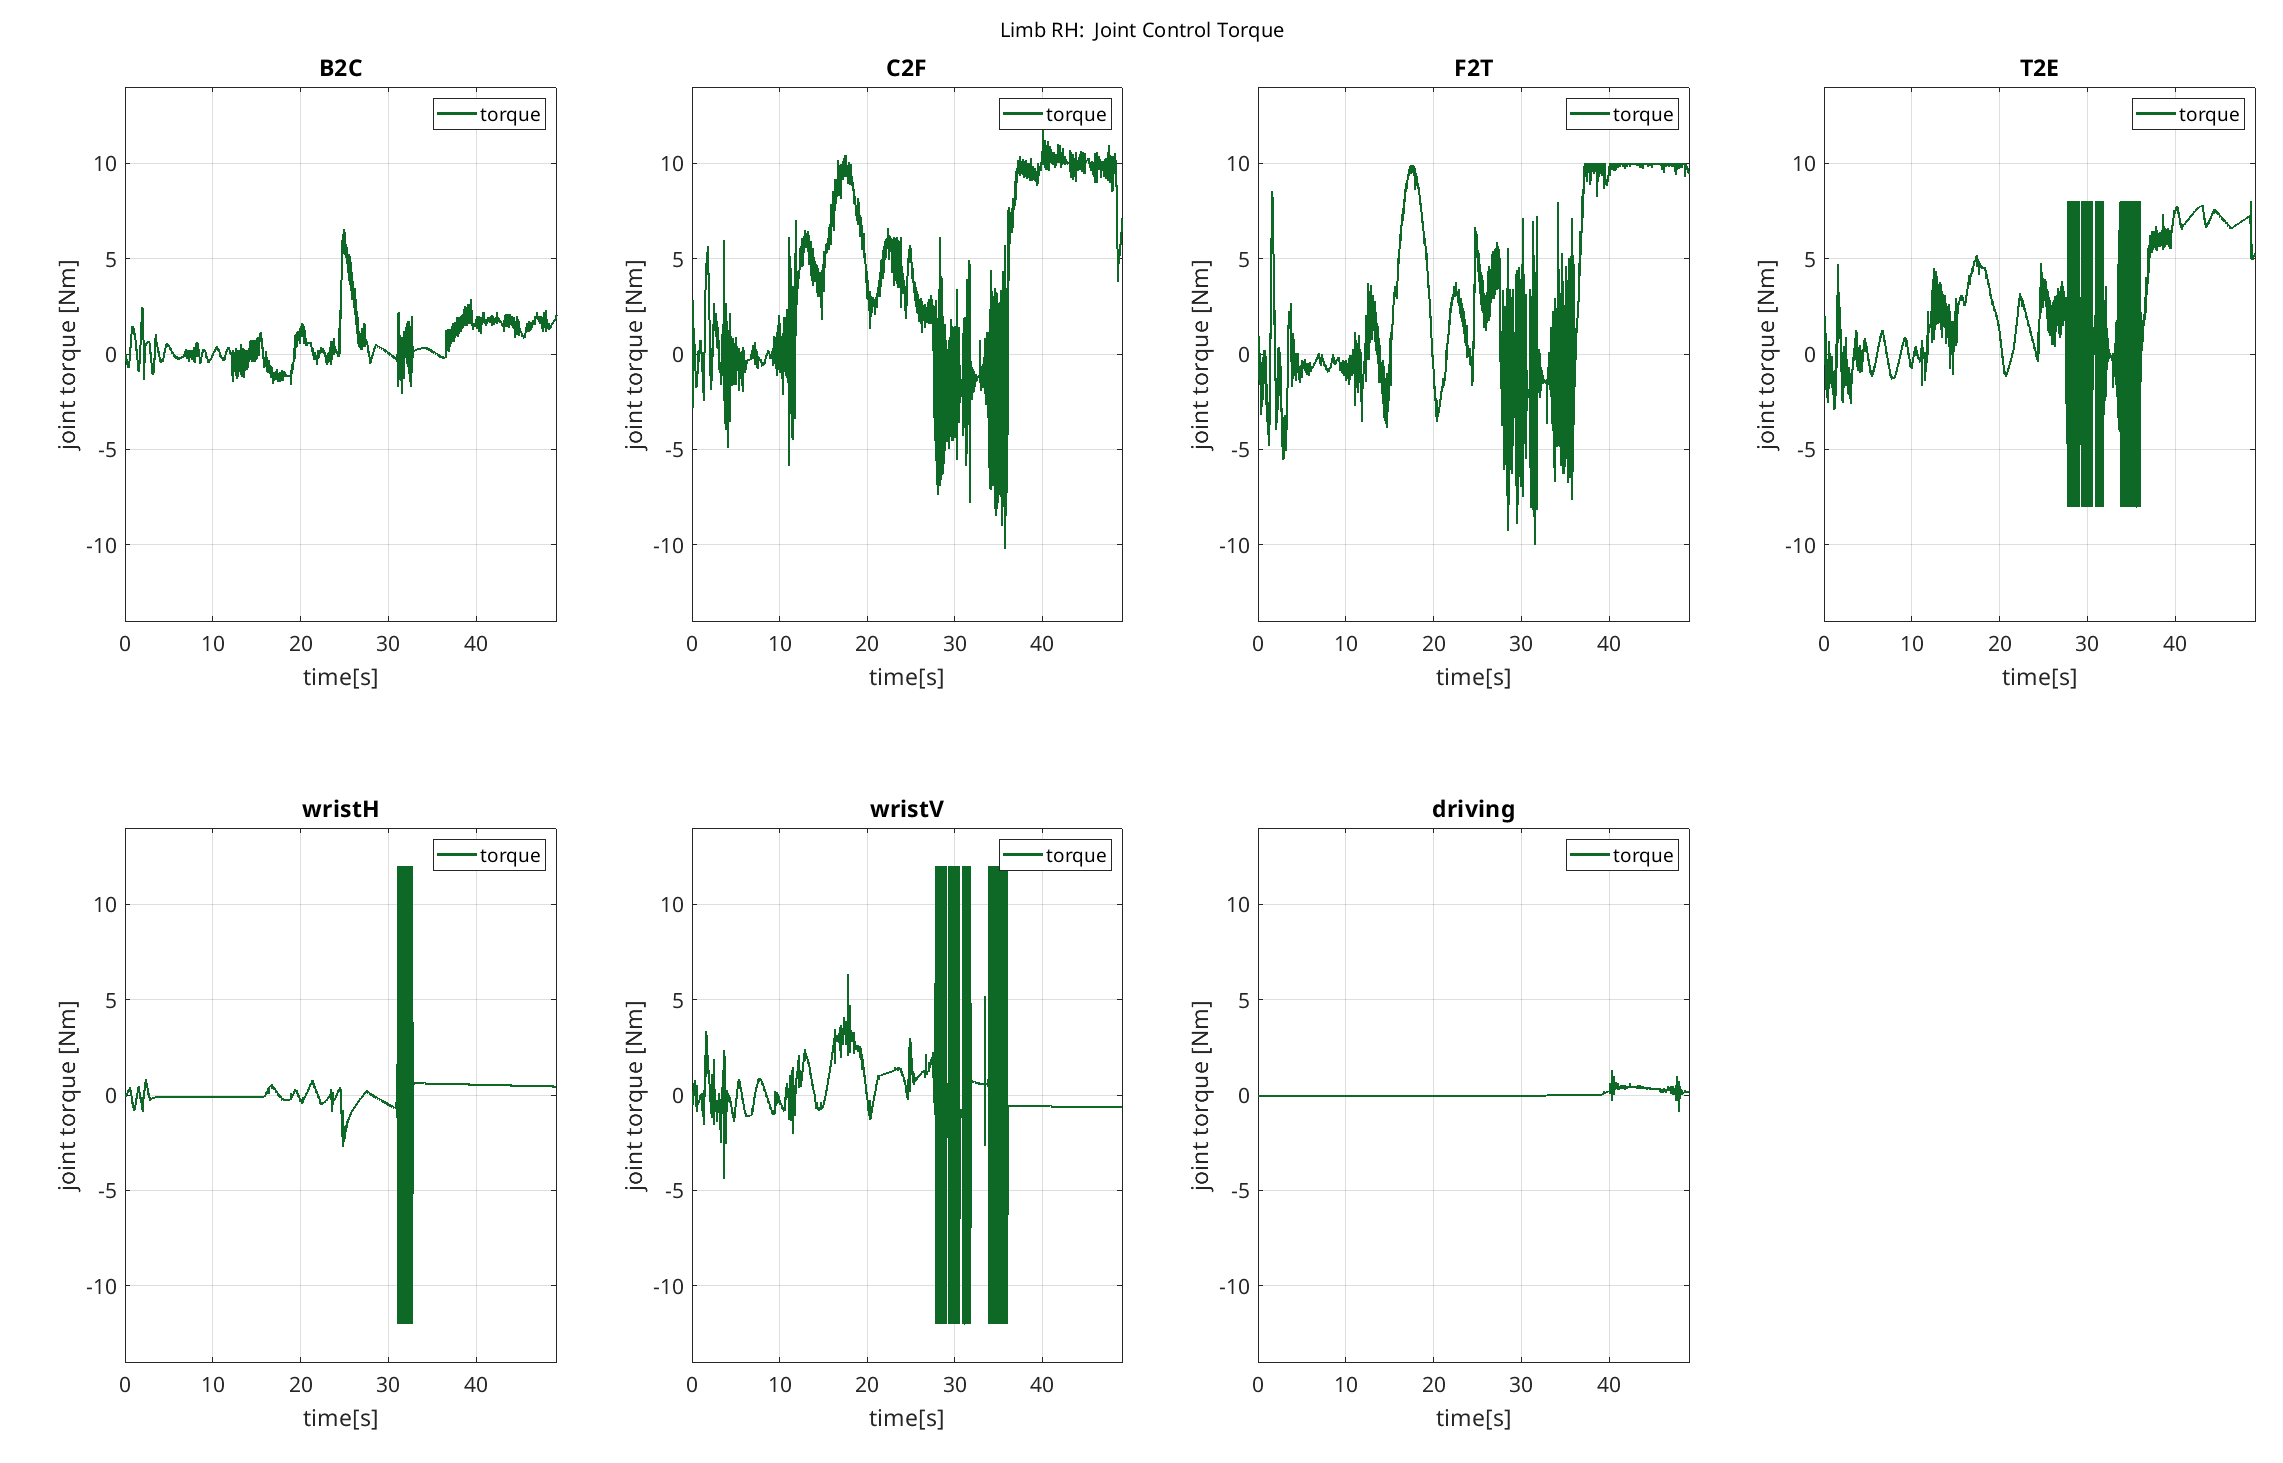
\includegraphics[width=1.0\textwidth]{Images/img_ch8/G2W_RH_torque.png}
    \caption{RH limb, Joint torques during G2W}
    \label{fig:G2W_RH_harmonic_torque}
\end{figure}

\begin{figure}[H]
    \centering
    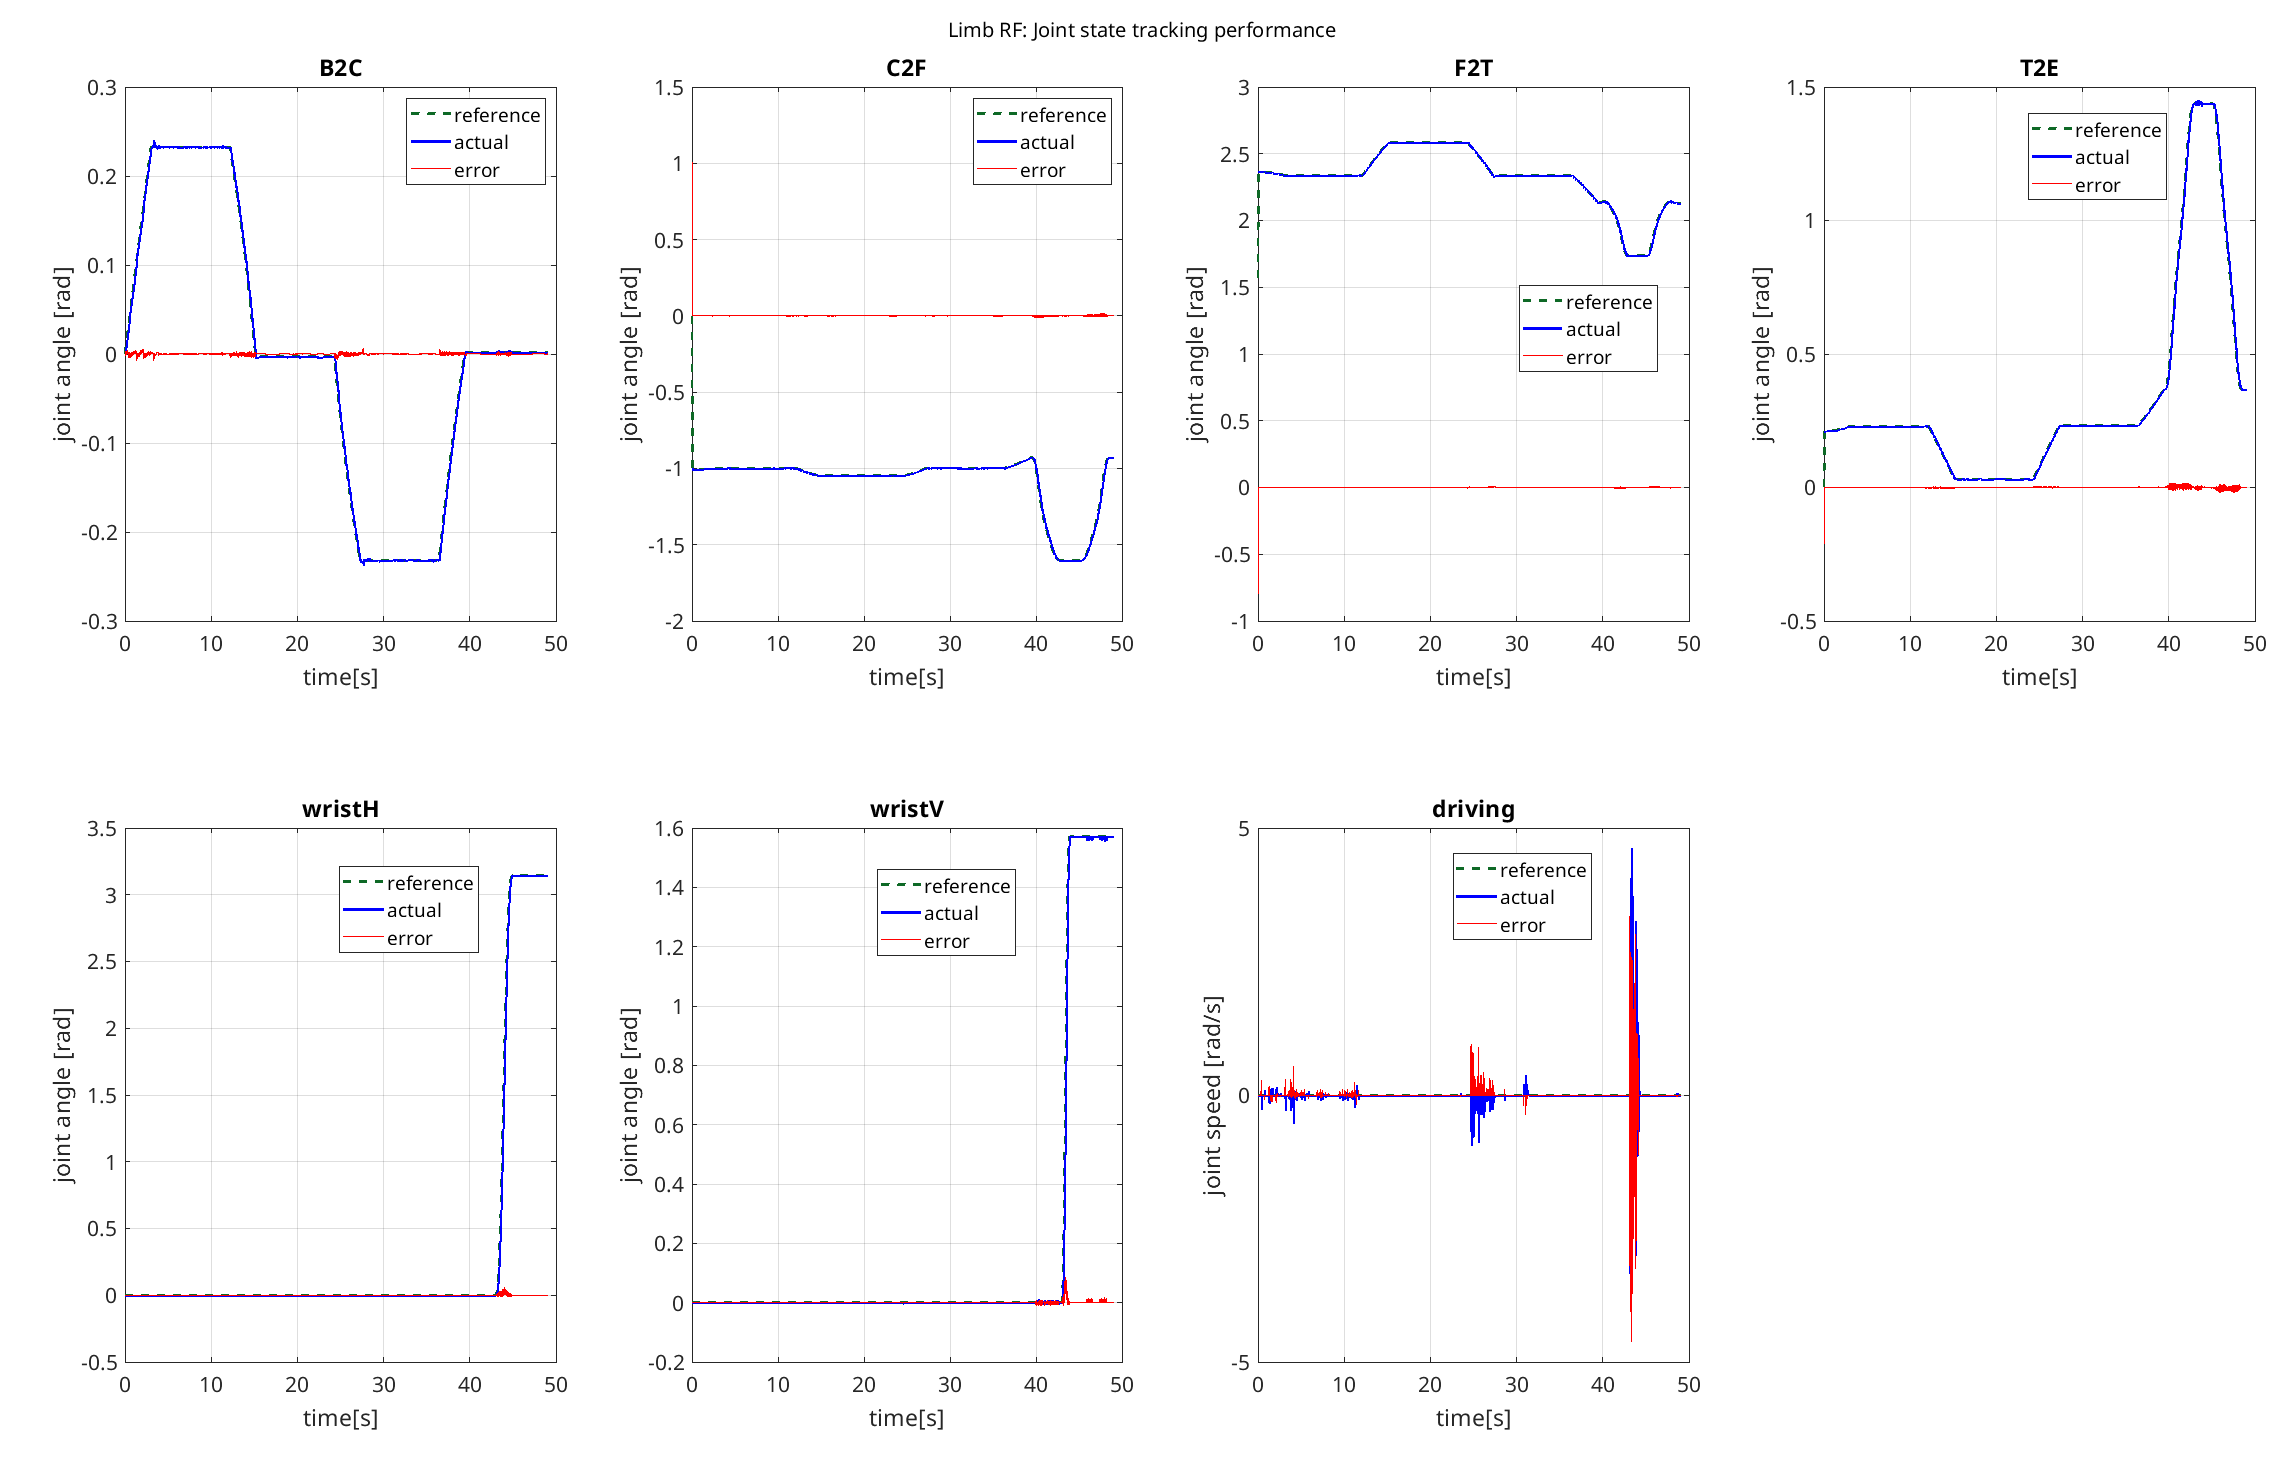
\includegraphics[width=1.0\textwidth]{Images/img_ch8/G2W_RF_joints.png}
    \caption{RF limb, Joint tracking during G2W}
    \label{fig:G2W_RF_harmonic_joint}
\end{figure}

\begin{figure}[H]
    \centering
    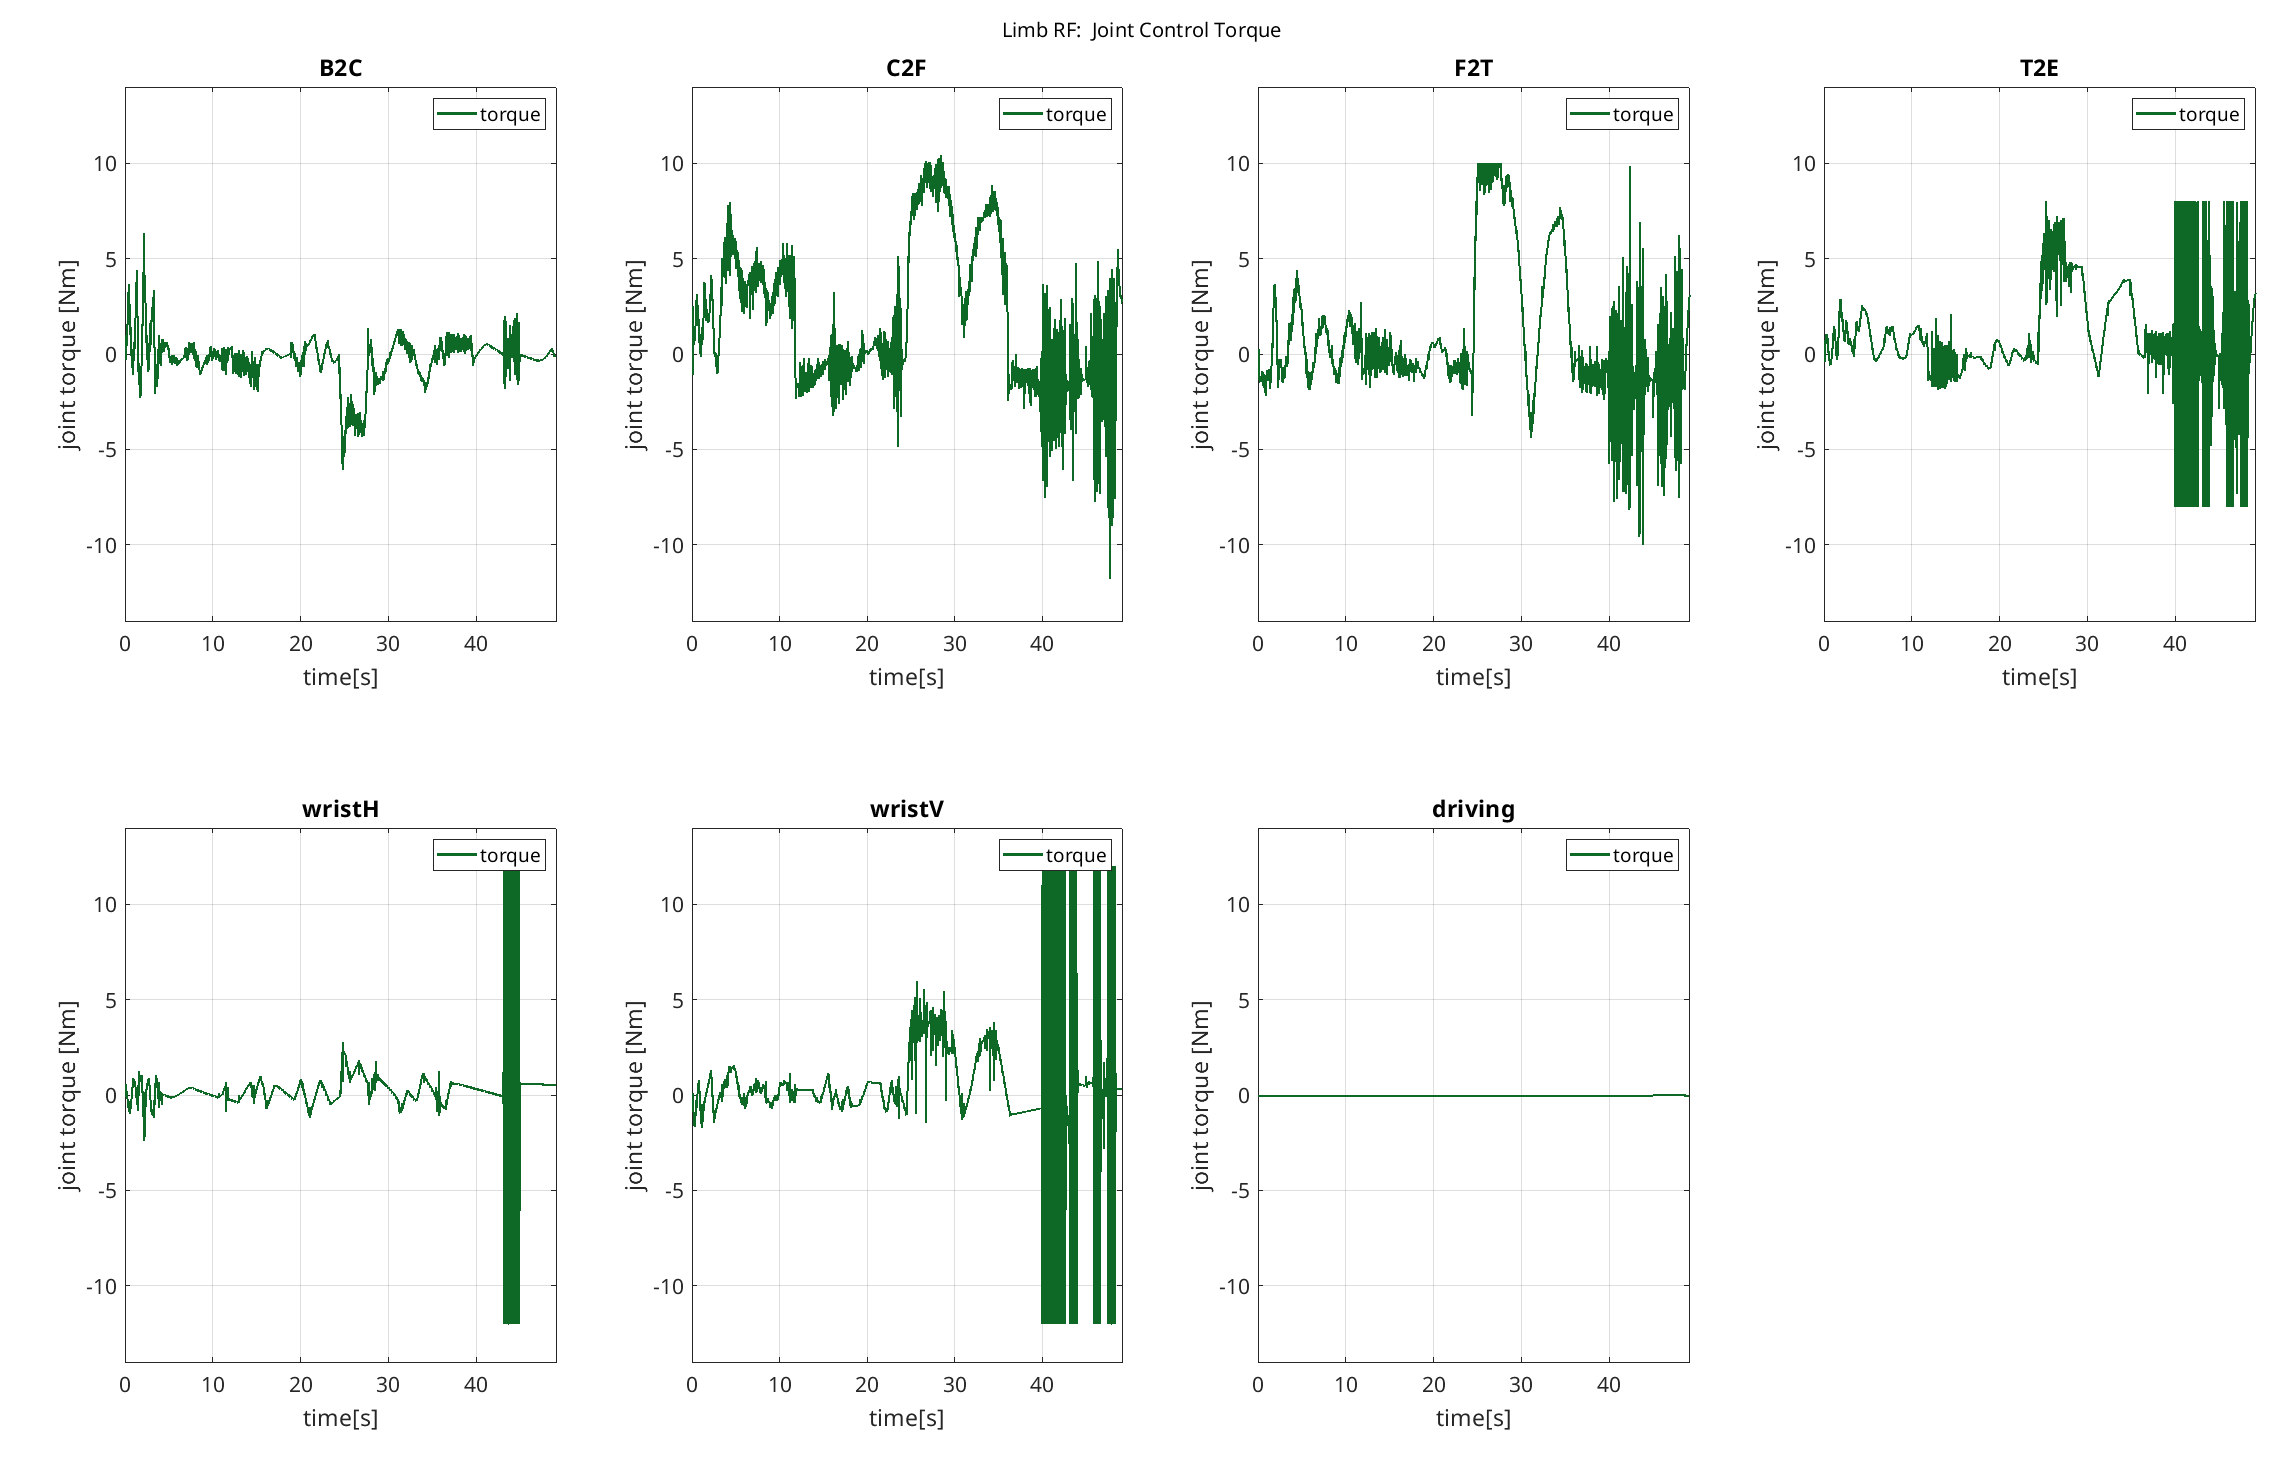
\includegraphics[width=1.0\textwidth]{Images/img_ch8/G2W_RF_torque.png}
    \caption{RF limb, Joint torques during G2W}
    \label{fig:G2W_RF_harmonic_torque}
\end{figure}

\begin{figure}[H]
    \centering
    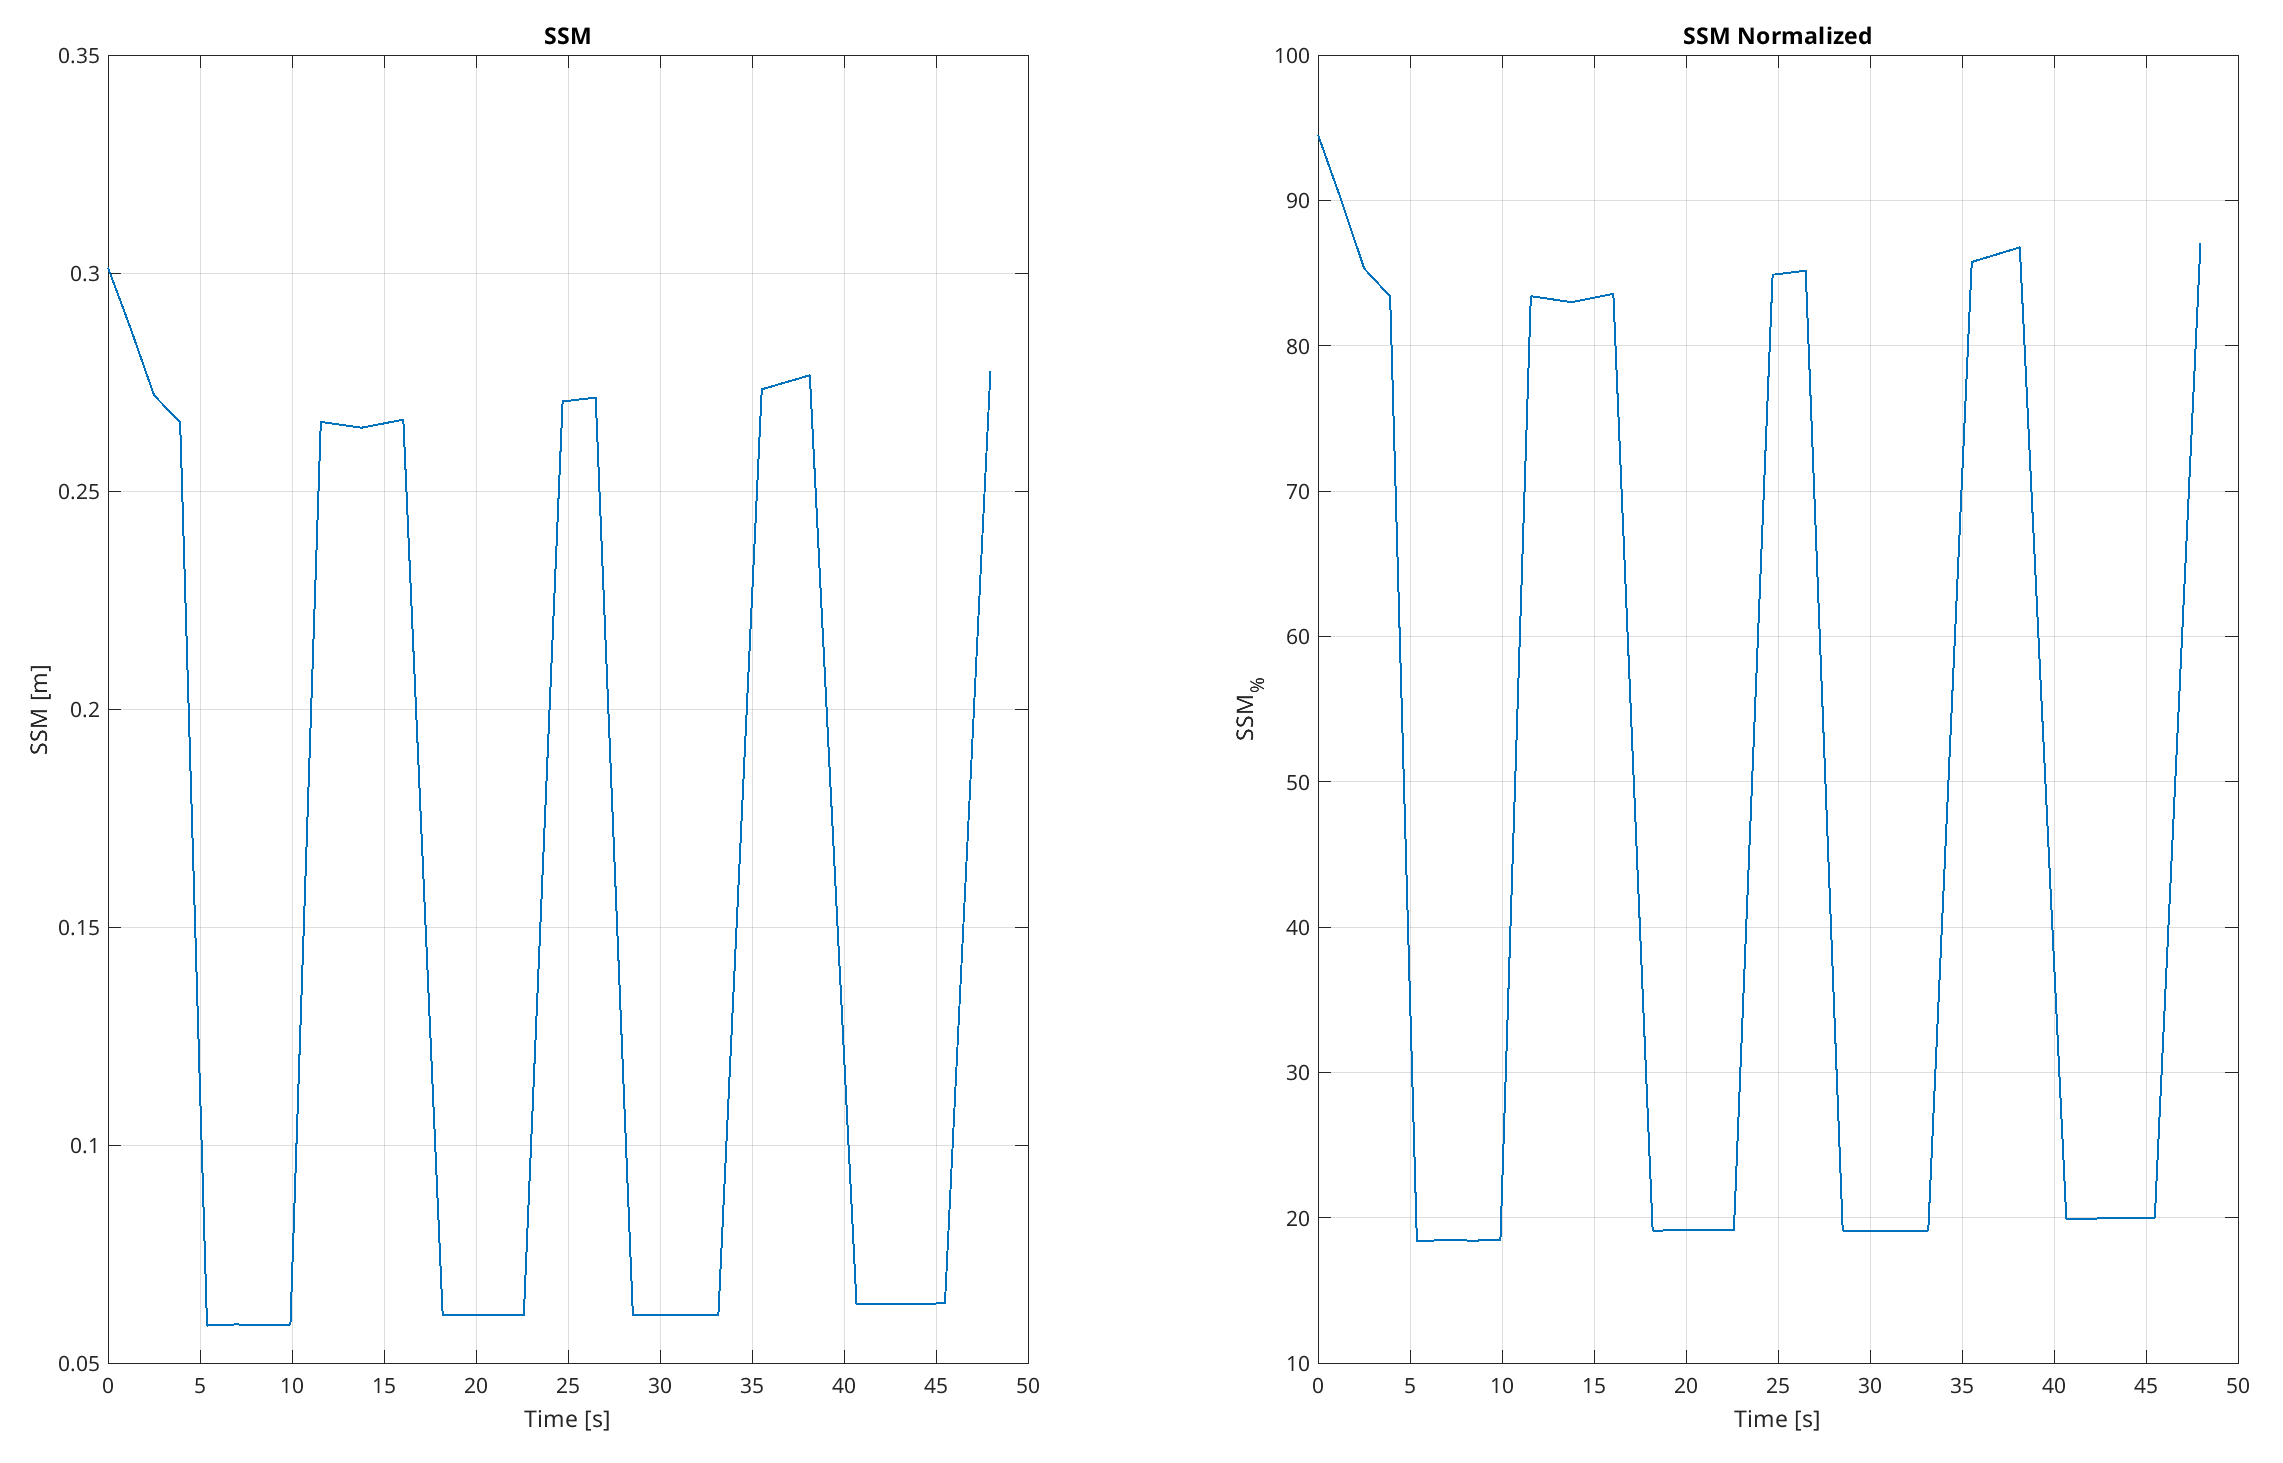
\includegraphics[width=0.9\textwidth]{Images/img_ch8/G2W_SSM.png}
    \caption{SSM and $SSM_\%$, during G2W}
    \label{fig:G2W_SSM_harmonic}
\end{figure}

\newpage
%% --- DRIVING ---
\subsection{Driving}
\label{sec:gz_harmonic_driving}

Some steps of the driving tests in the simulator are shown in Fig.\ref{fig:G2W_harmonic}. 
In particular, in this tests on wheel mode, the following locomotion sequence has been performed and analyzed: 
\begin{enumerate}
    \setlength\itemsep{-0.7em} 
    \item 4-wheeled forward driving for 3 seconds
    \item LF W2G transformation
    \item 3-wheeled forward driving
\end{enumerate}
a sequence of 4-wheeled driving locomotion for 3 seconds, followed by a transformation of the LF limb and then  
The driving joint rotation velocity and the driving control torque are shown in Fig.\ref{fig:driving_performance}.
- \ref{fig:G2W_RF_harmonic_joint}, while the control torque computed by the IJCs is represented in Figs.\ref{fig:driving_LF_harmonic_torque} - \ref{fig:driving_RF_harmonic_torque}.
In conclusion, Stability margins during the driving tests are reported in Fig.\ref{fig:driving_SSM_harmonic}. 

\begin{figure}[H]
    \centering
    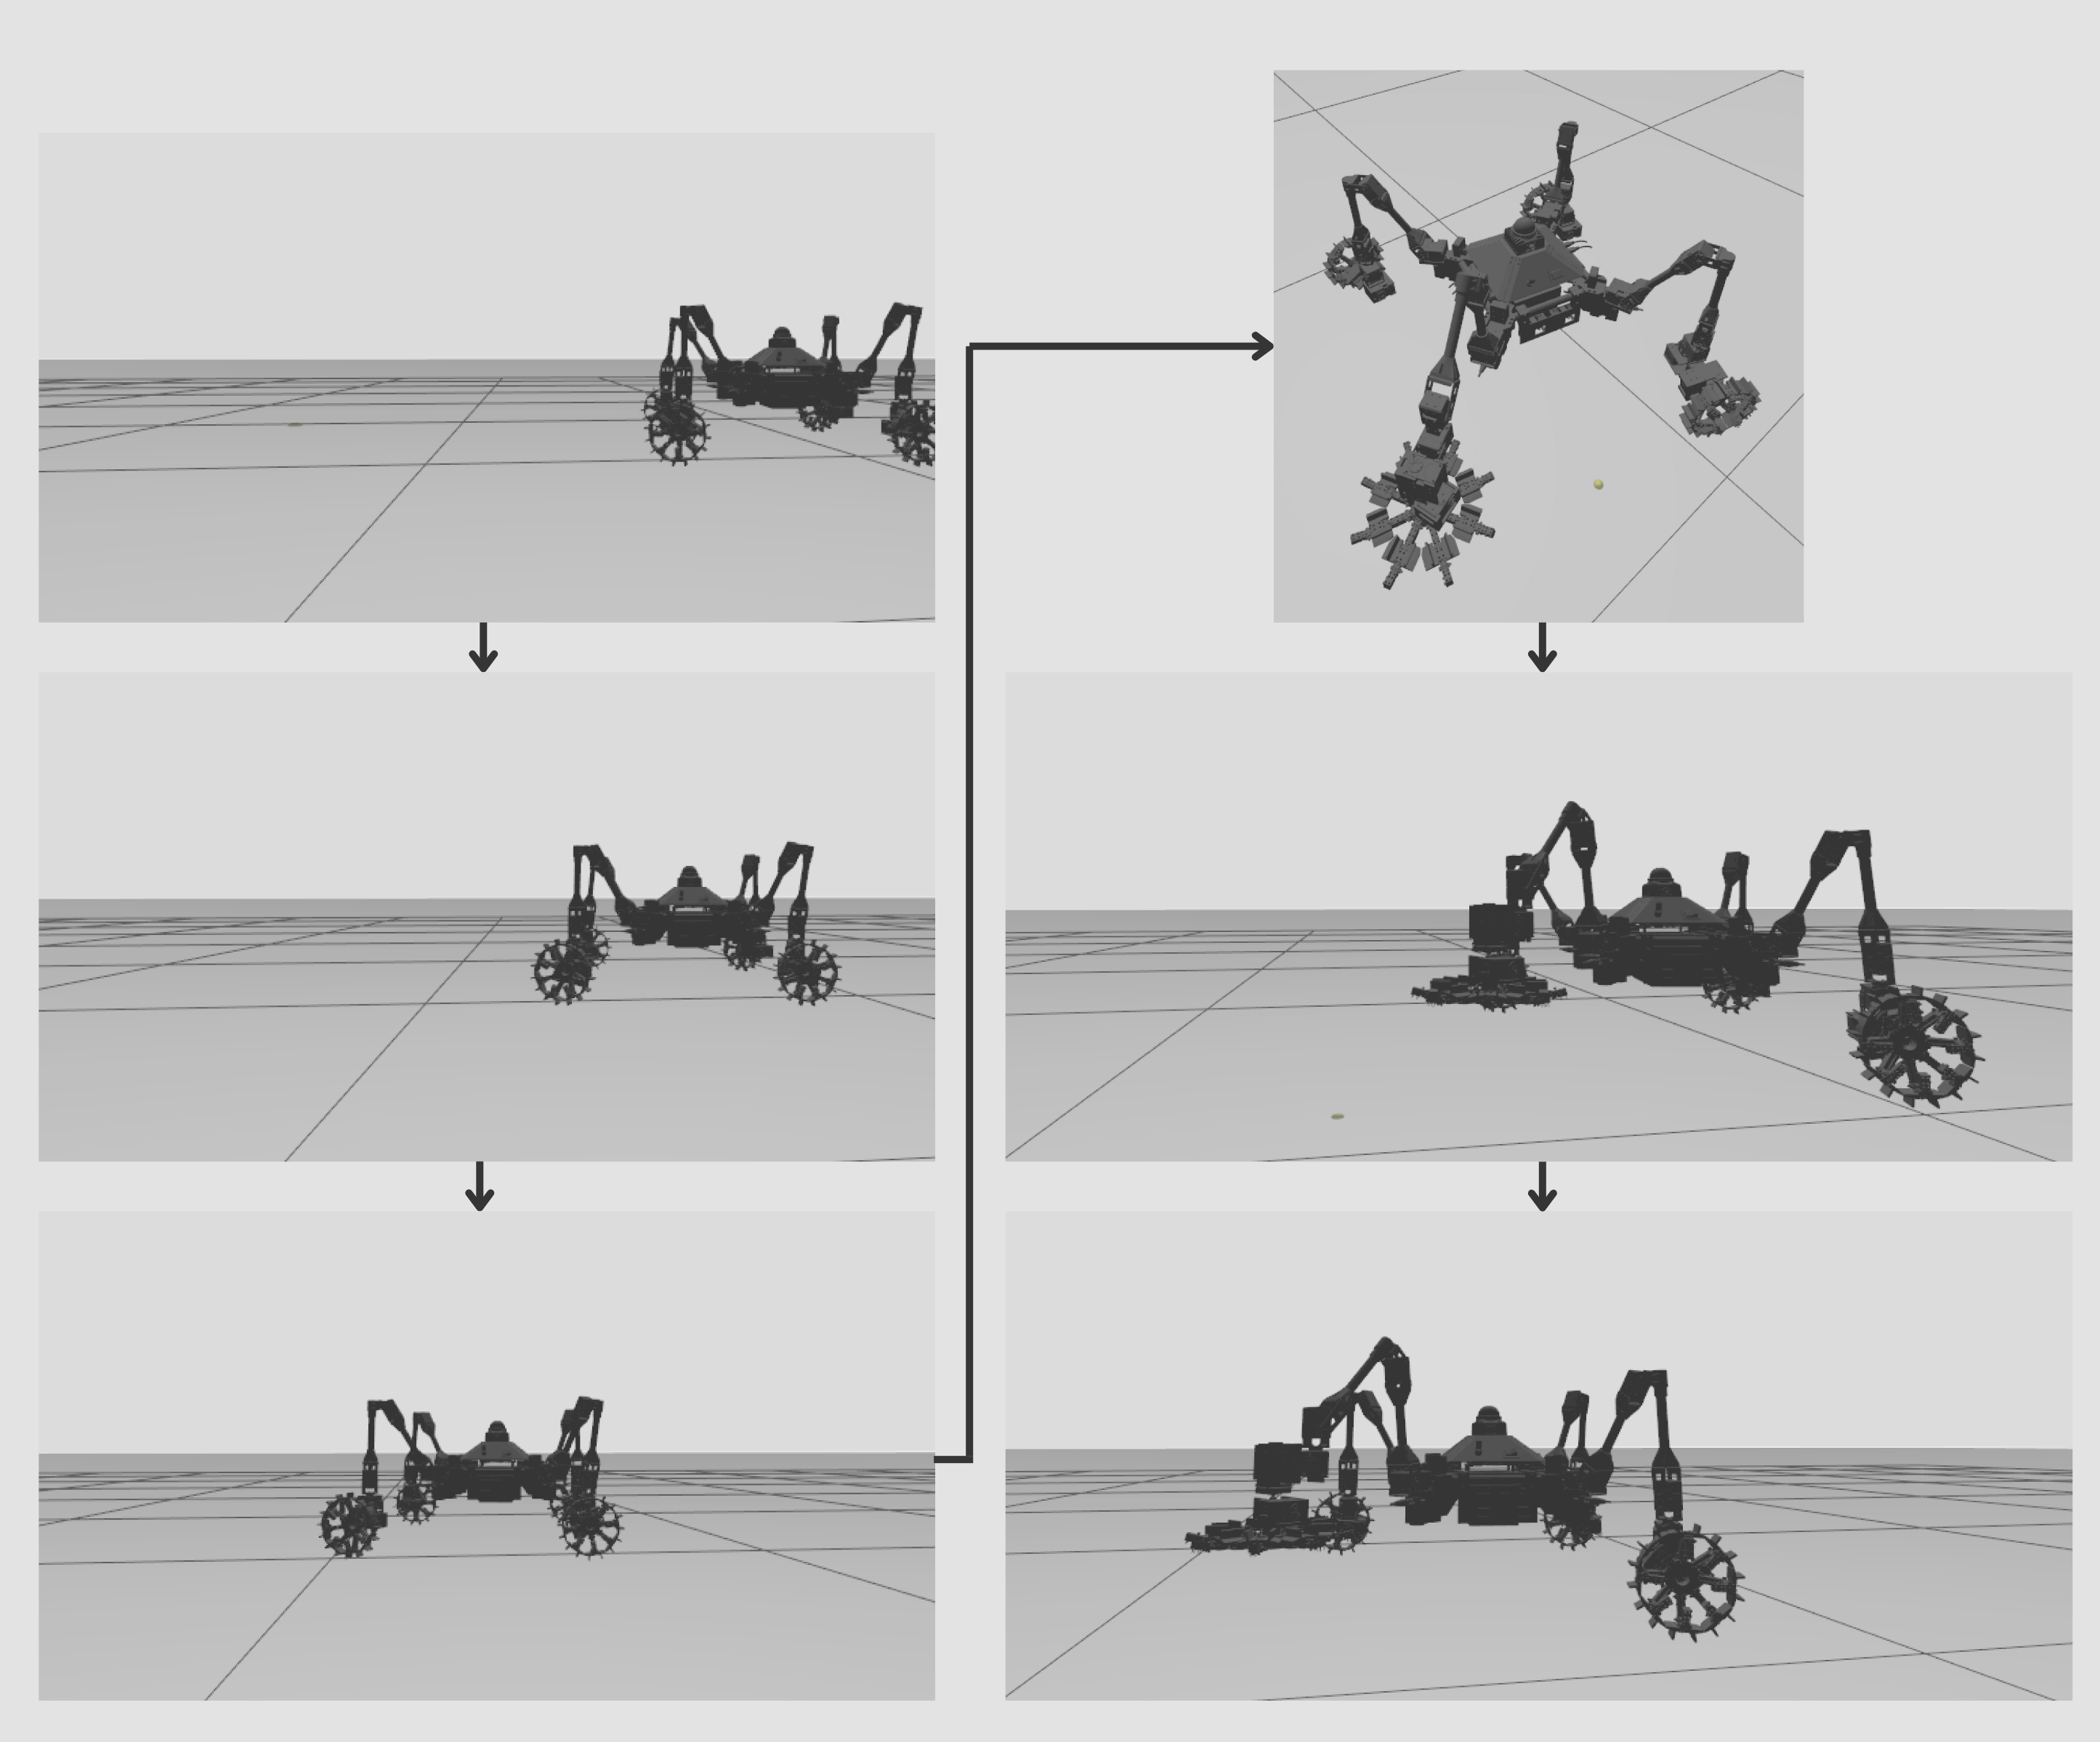
\includegraphics[width=0.9\textwidth]{Images/img_ch8/driving_sim.png}
    \caption{driving with four or three support wheels in Gazebo Harmonic}
    \label{driving_harmonic}
\end{figure}

\begin{figure}[H]
    \centering
    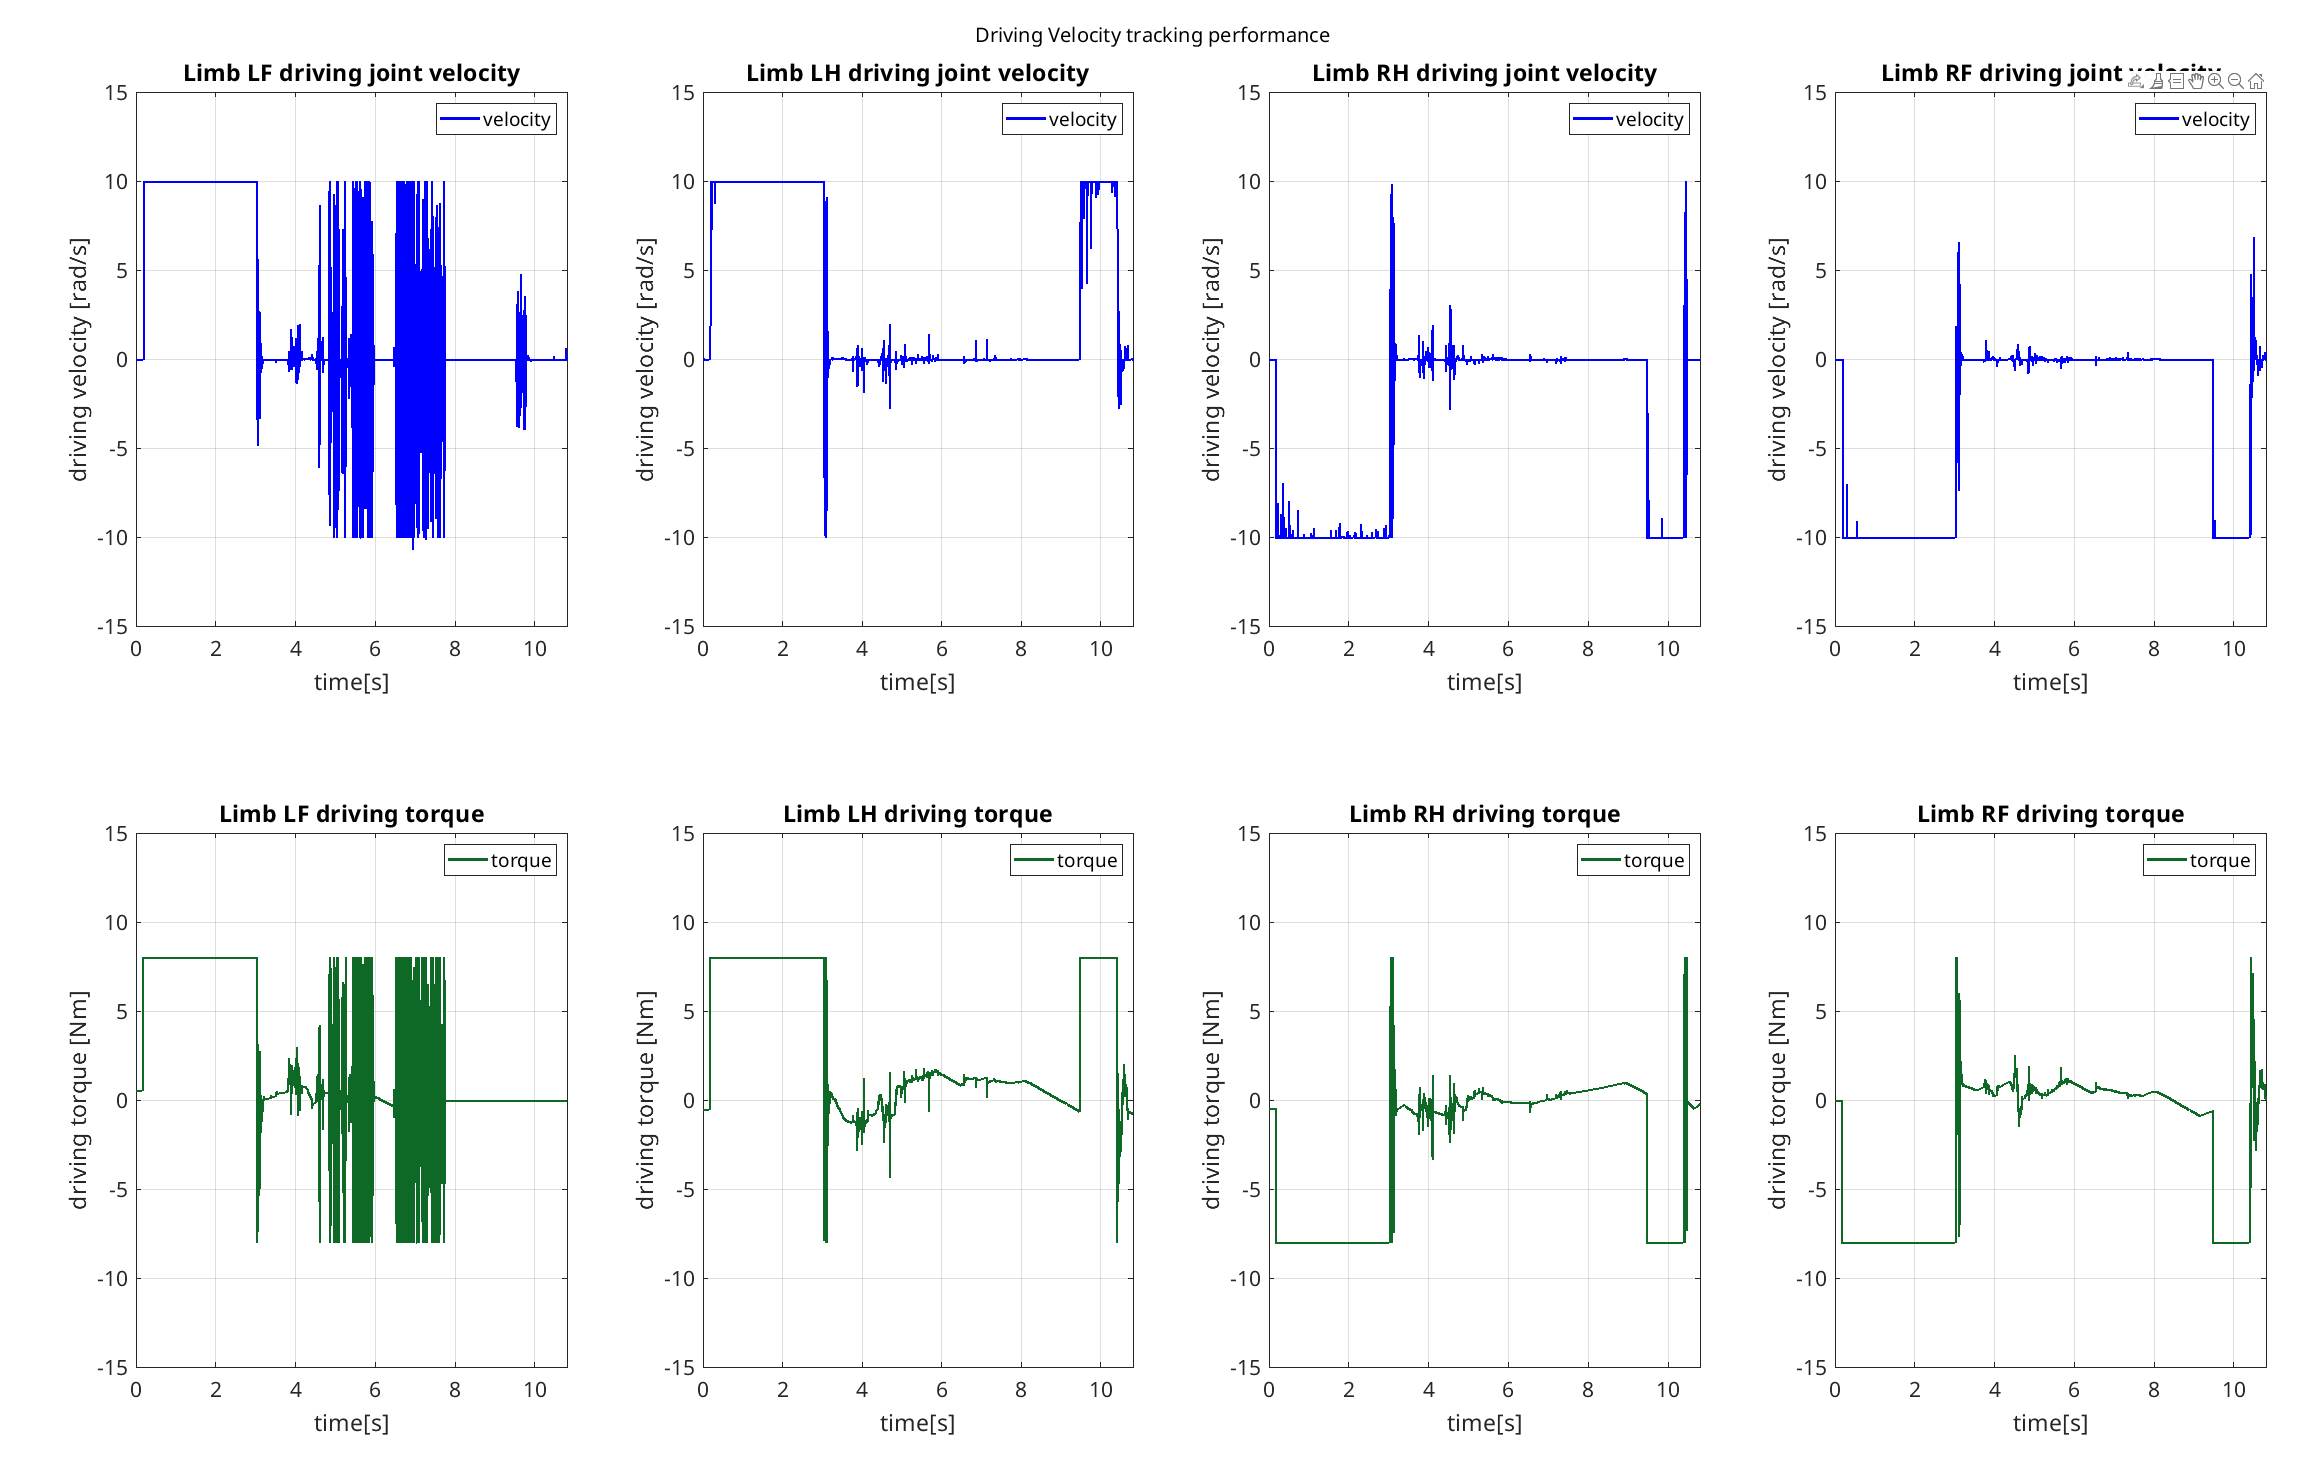
\includegraphics[width=1.0\textwidth]{Images/img_ch8/driving_performance.png}
    \caption{Driving joint rotational velocity, during driving test}
    \label{fig:driving_performance}
\end{figure}

\begin{figure}[H]
    \centering
    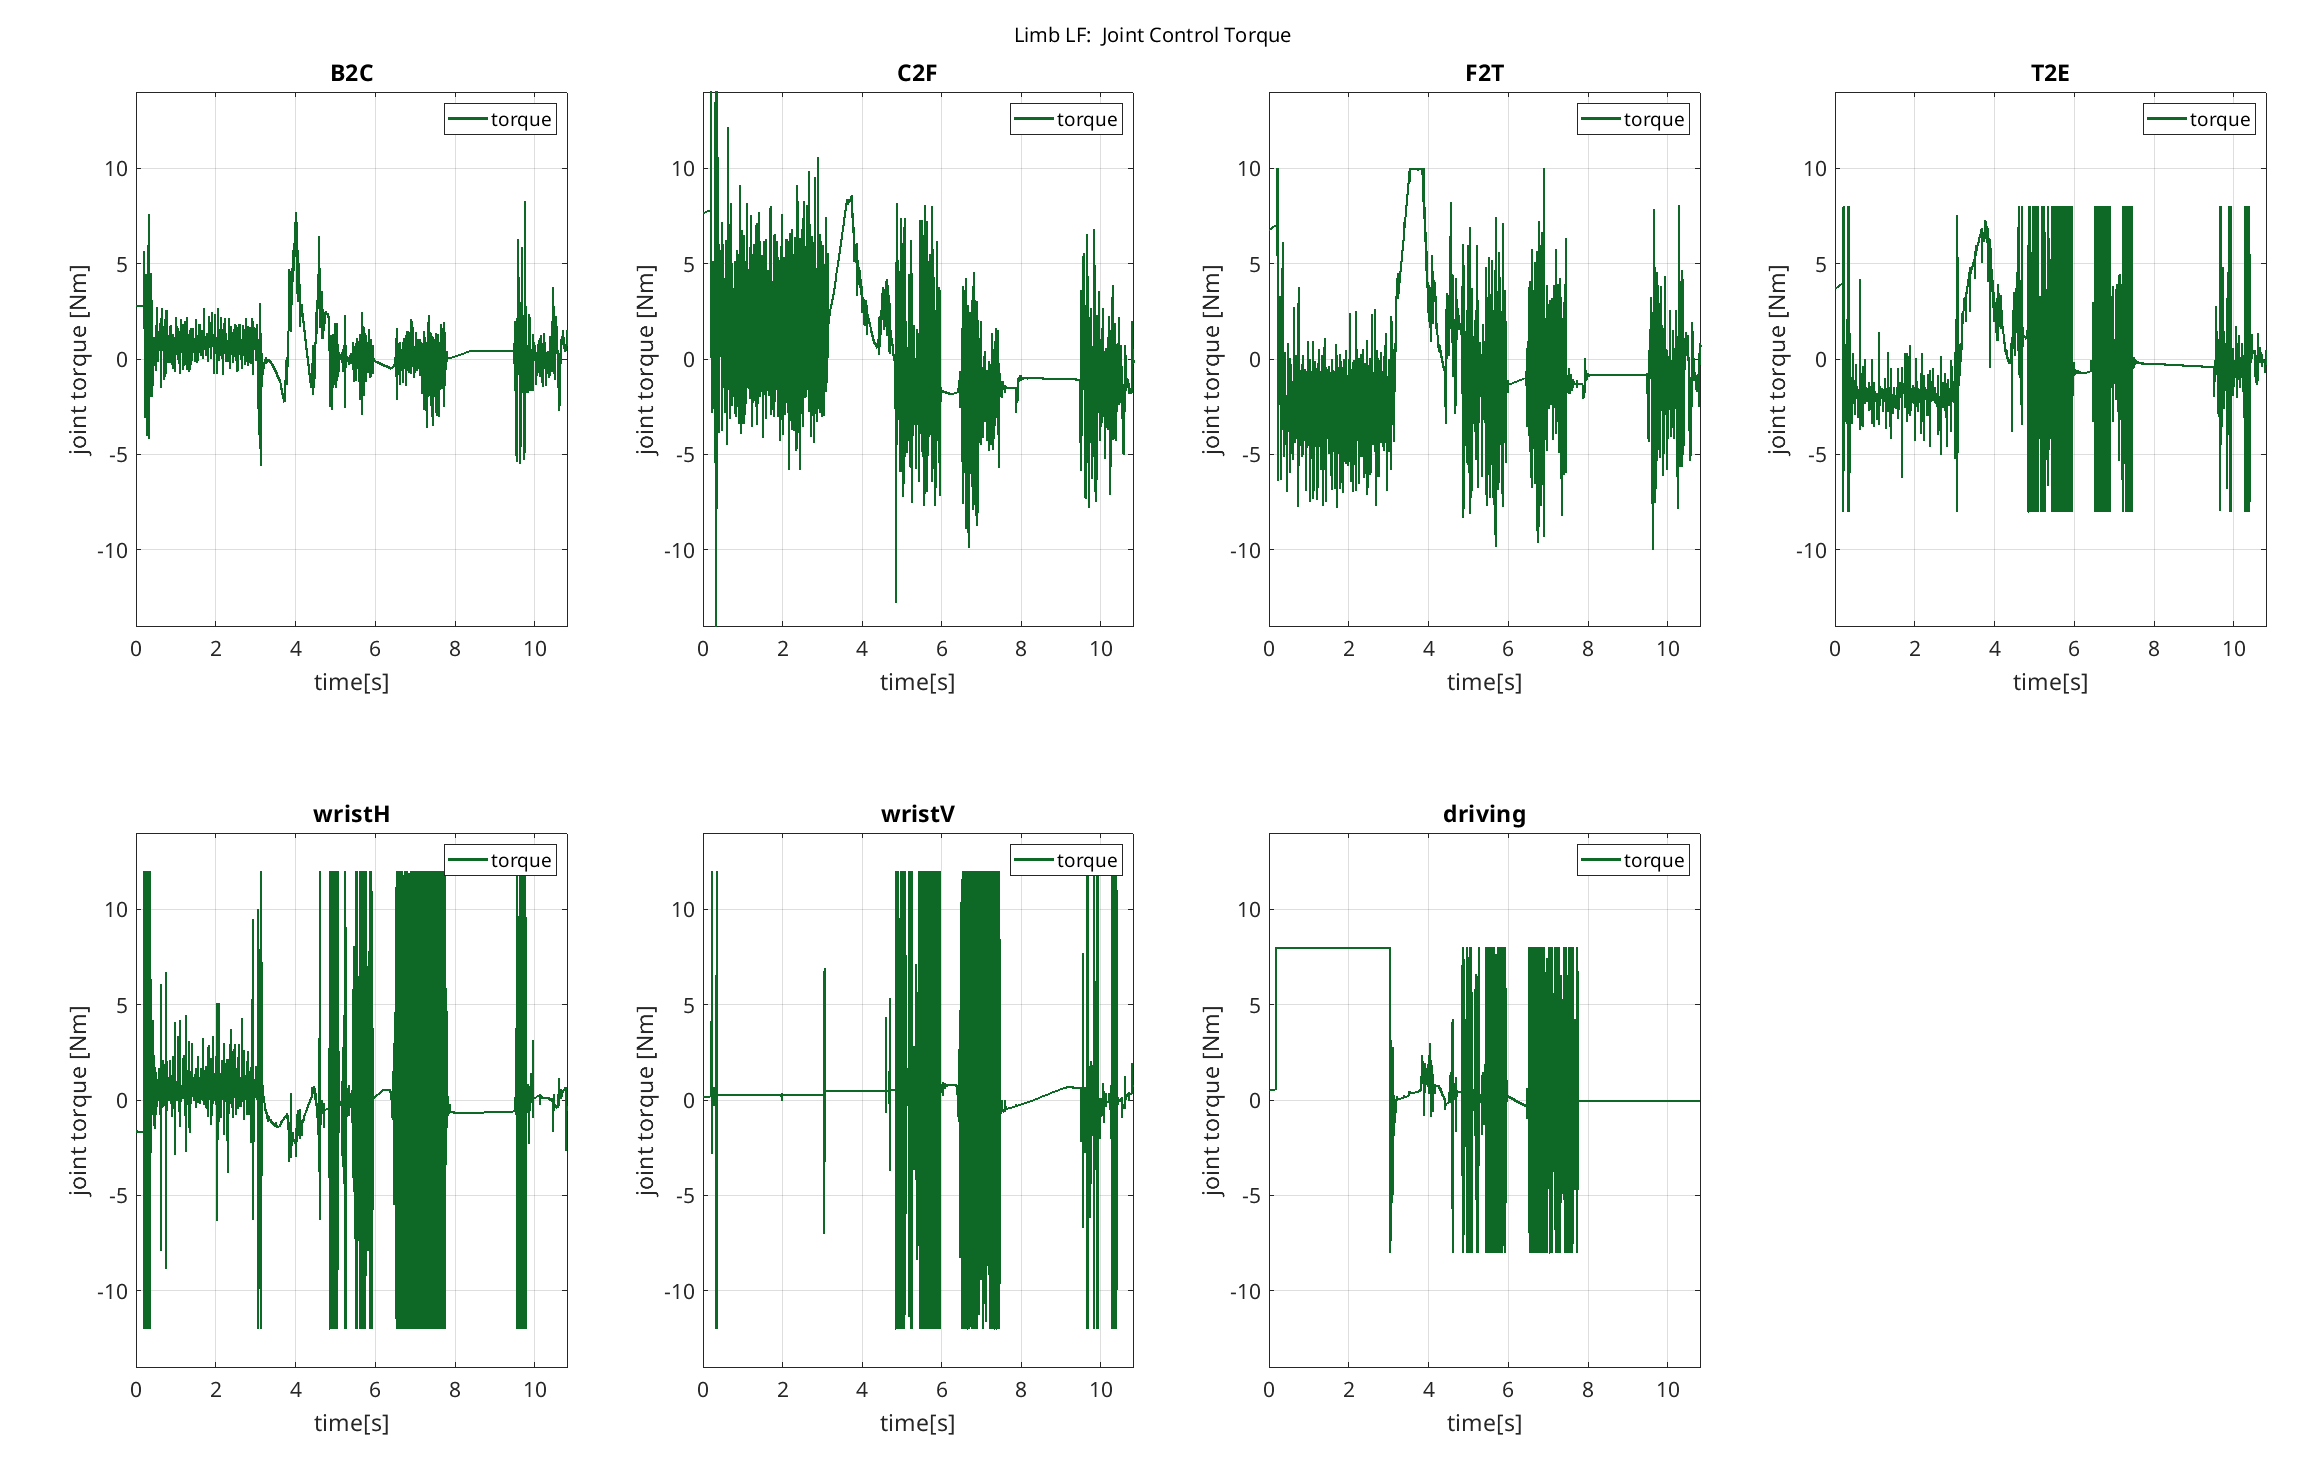
\includegraphics[width=1.0\textwidth]{Images/img_ch8/driving_LF_torque.png}
    \caption{LF limb, Joint torques during driving test}
    \label{fig:driving_LF_harmonic_torque}
\end{figure}

\begin{figure}[H]
    \centering
    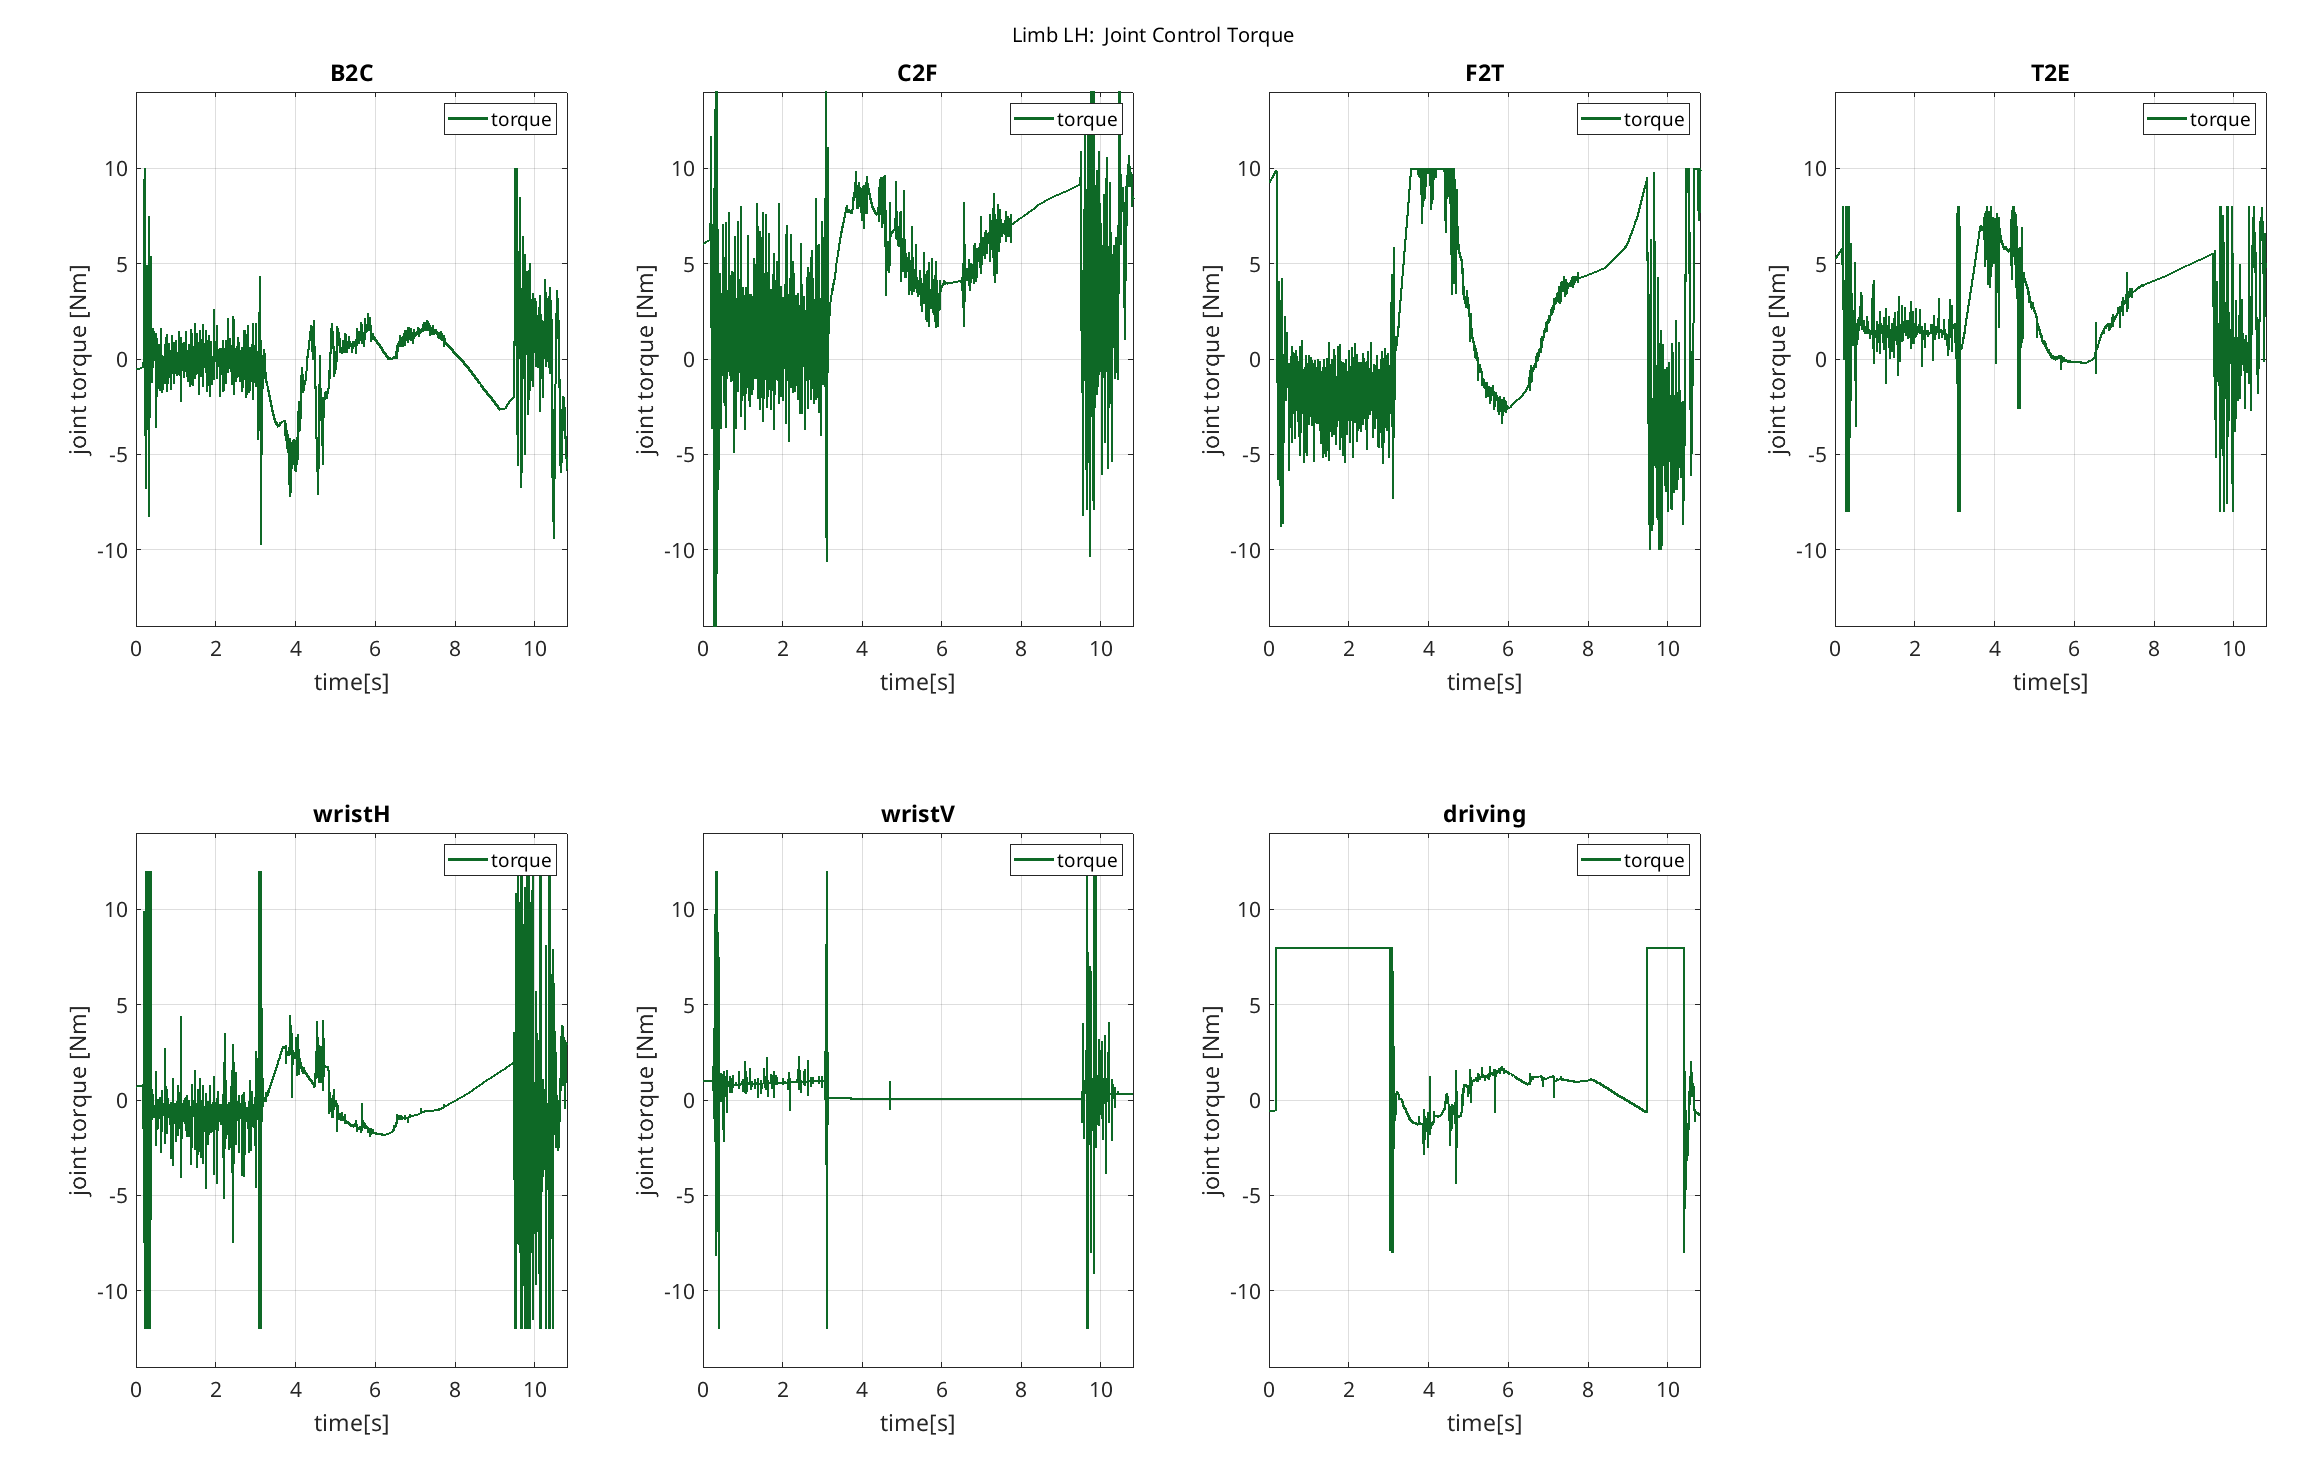
\includegraphics[width=1.0\textwidth]{Images/img_ch8/driving_LH_torque.png}
    \caption{LH limb, Joint torques during driving test}
    \label{fig:driving_LH_harmonic_torque}
\end{figure}

\begin{figure}[H]
    \centering
    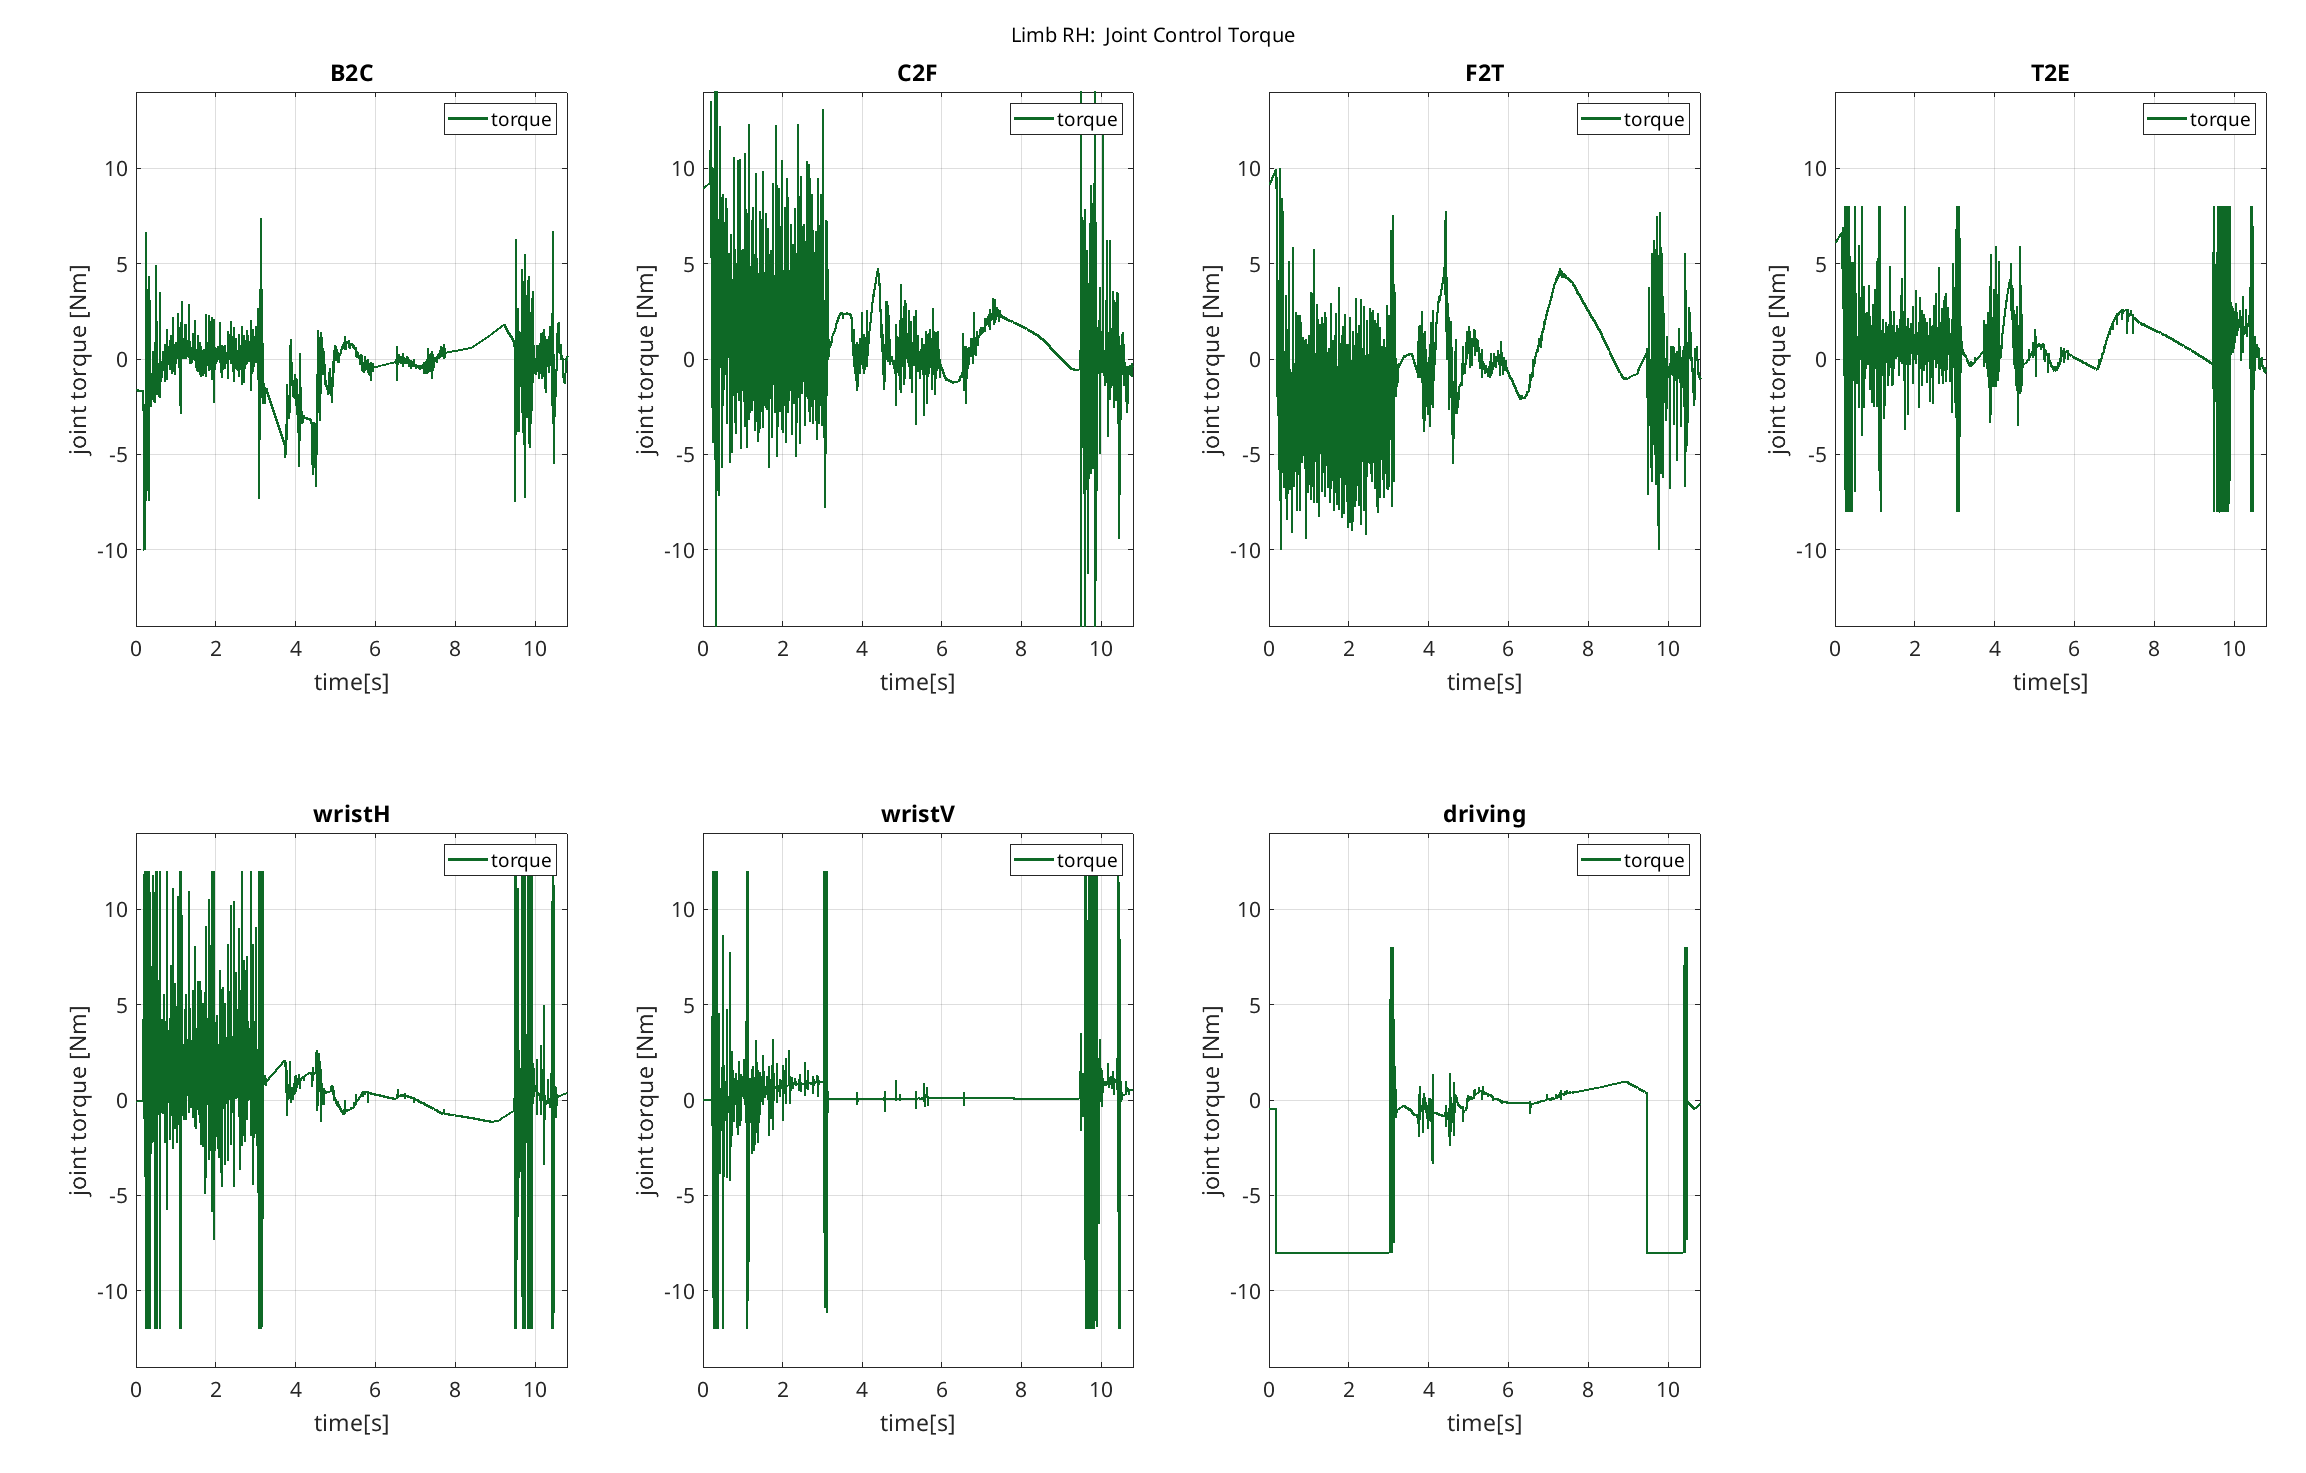
\includegraphics[width=1.0\textwidth]{Images/img_ch8/driving_RH_torque.png}
    \caption{RH limb, Joint torques during driving test}
    \label{fig:driving_RH_harmonic_torque}
\end{figure}
\begin{figure}[H]
    \centering
    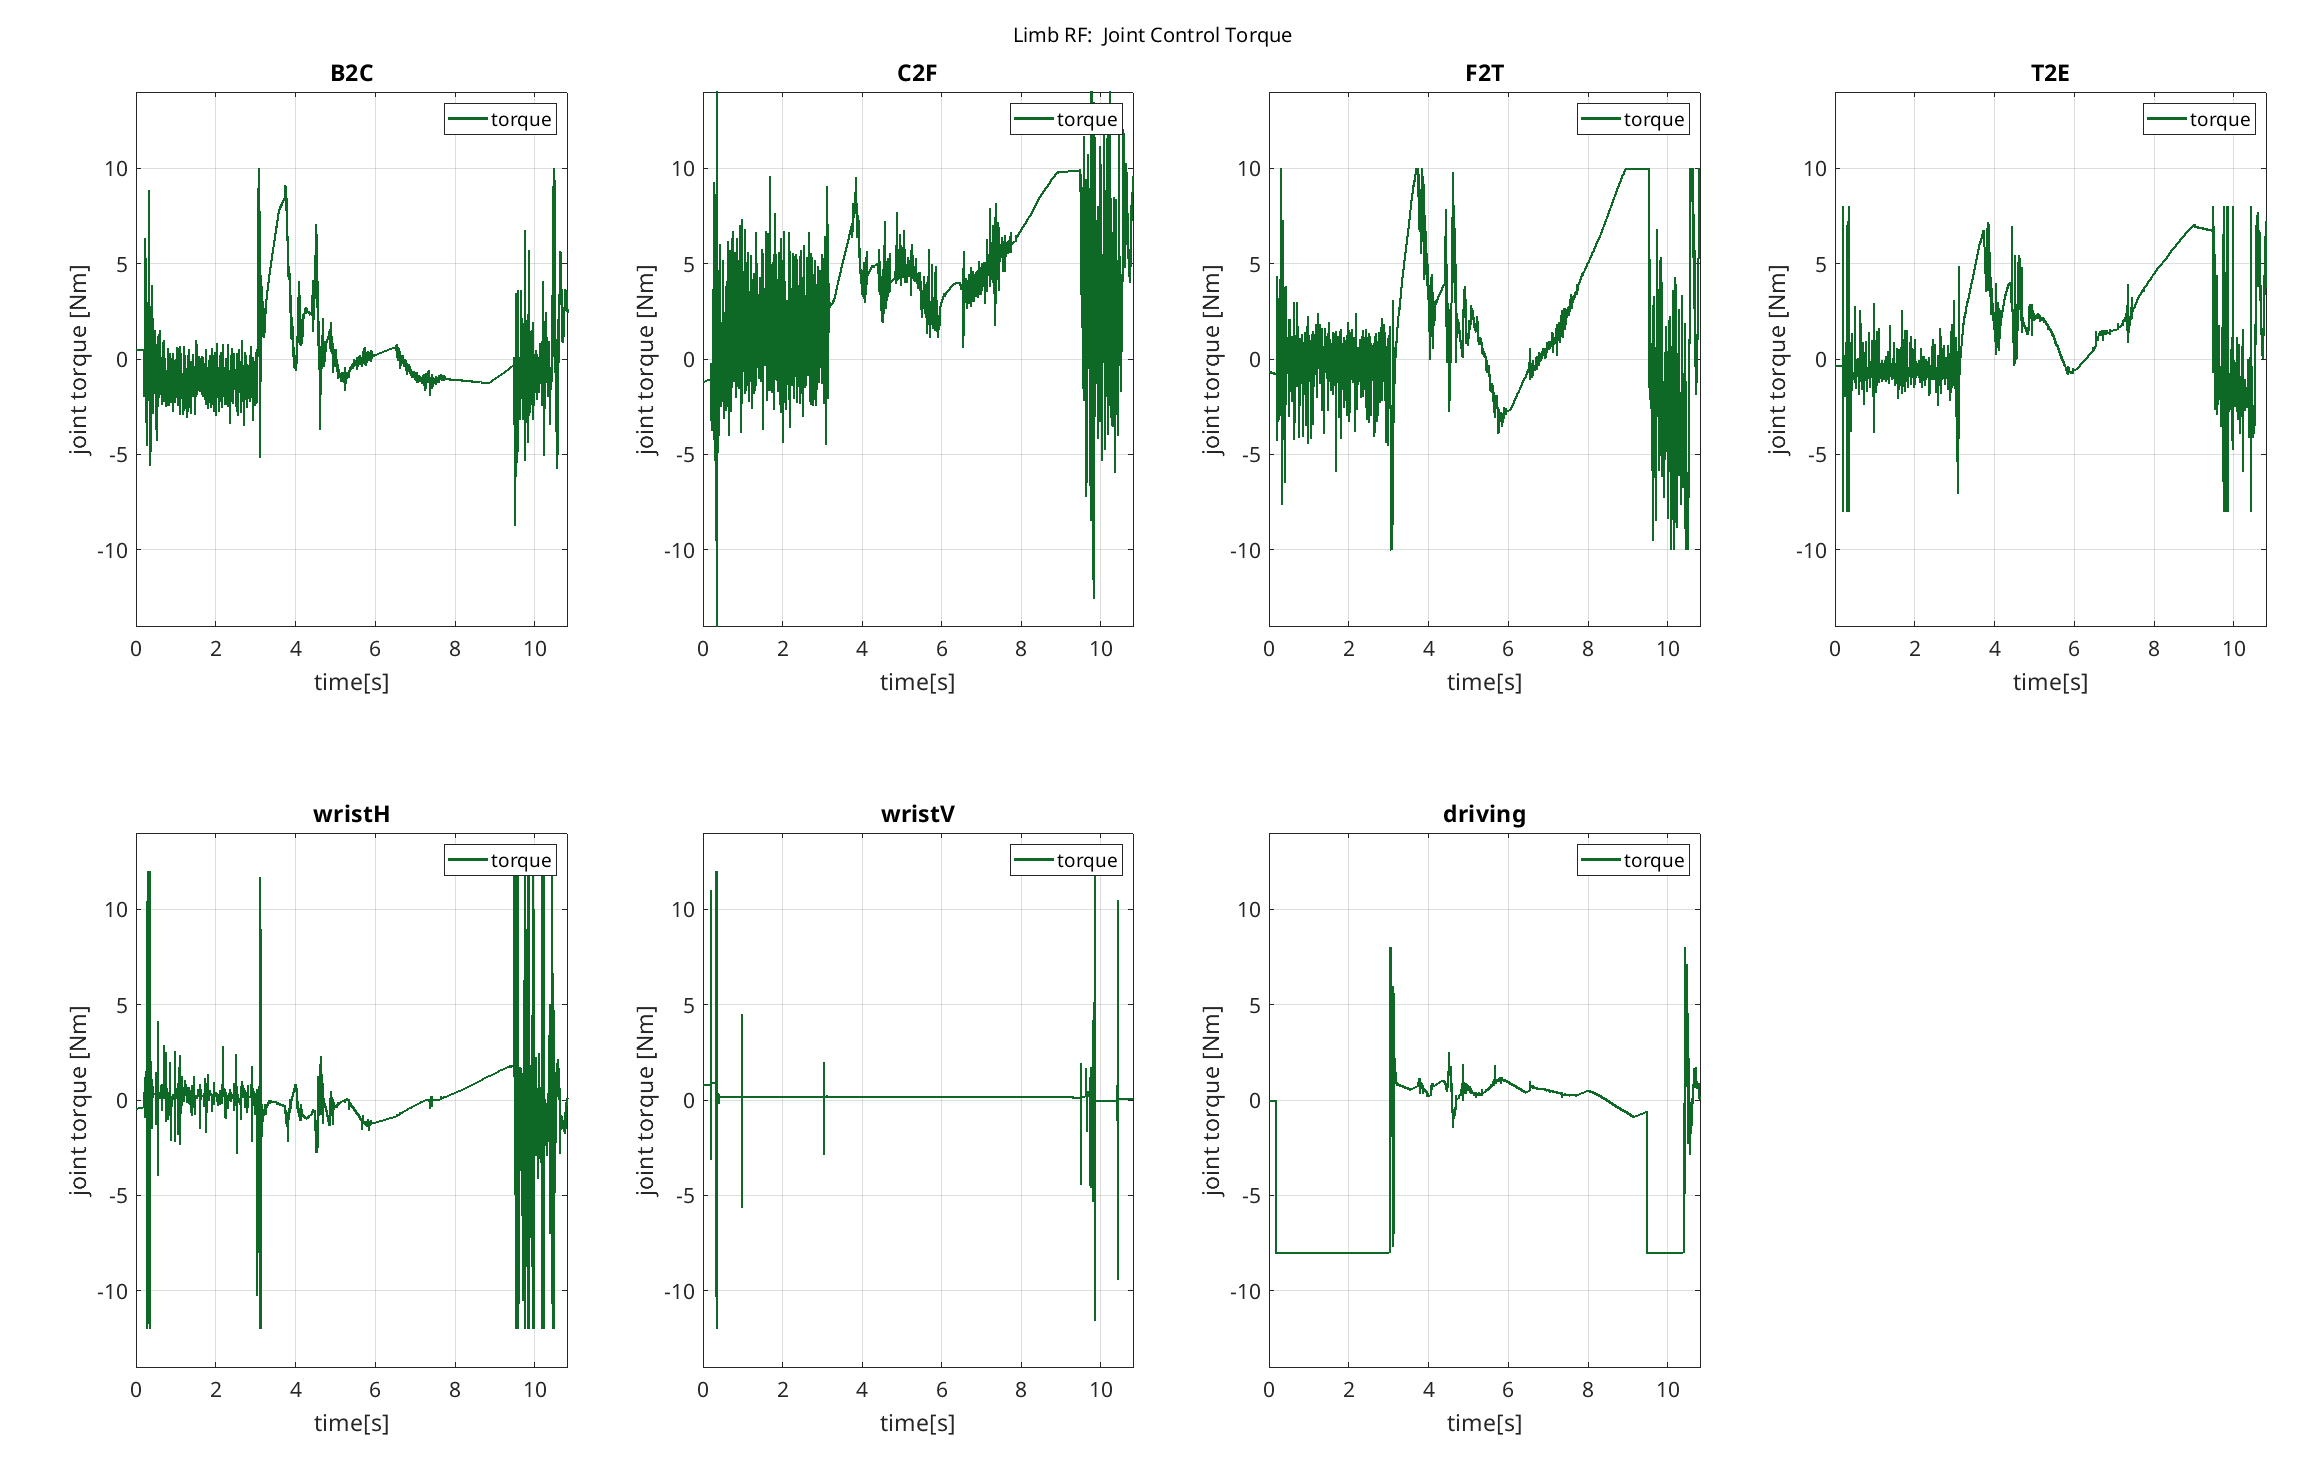
\includegraphics[width=1.0\textwidth]{Images/img_ch8/driving_RF_torque.png}
    \caption{RF limb, Joint torques during driving test}
    \label{fig:driving_RF_harmonic_torque}
\end{figure}
\begin{figure}[H]
    \centering
    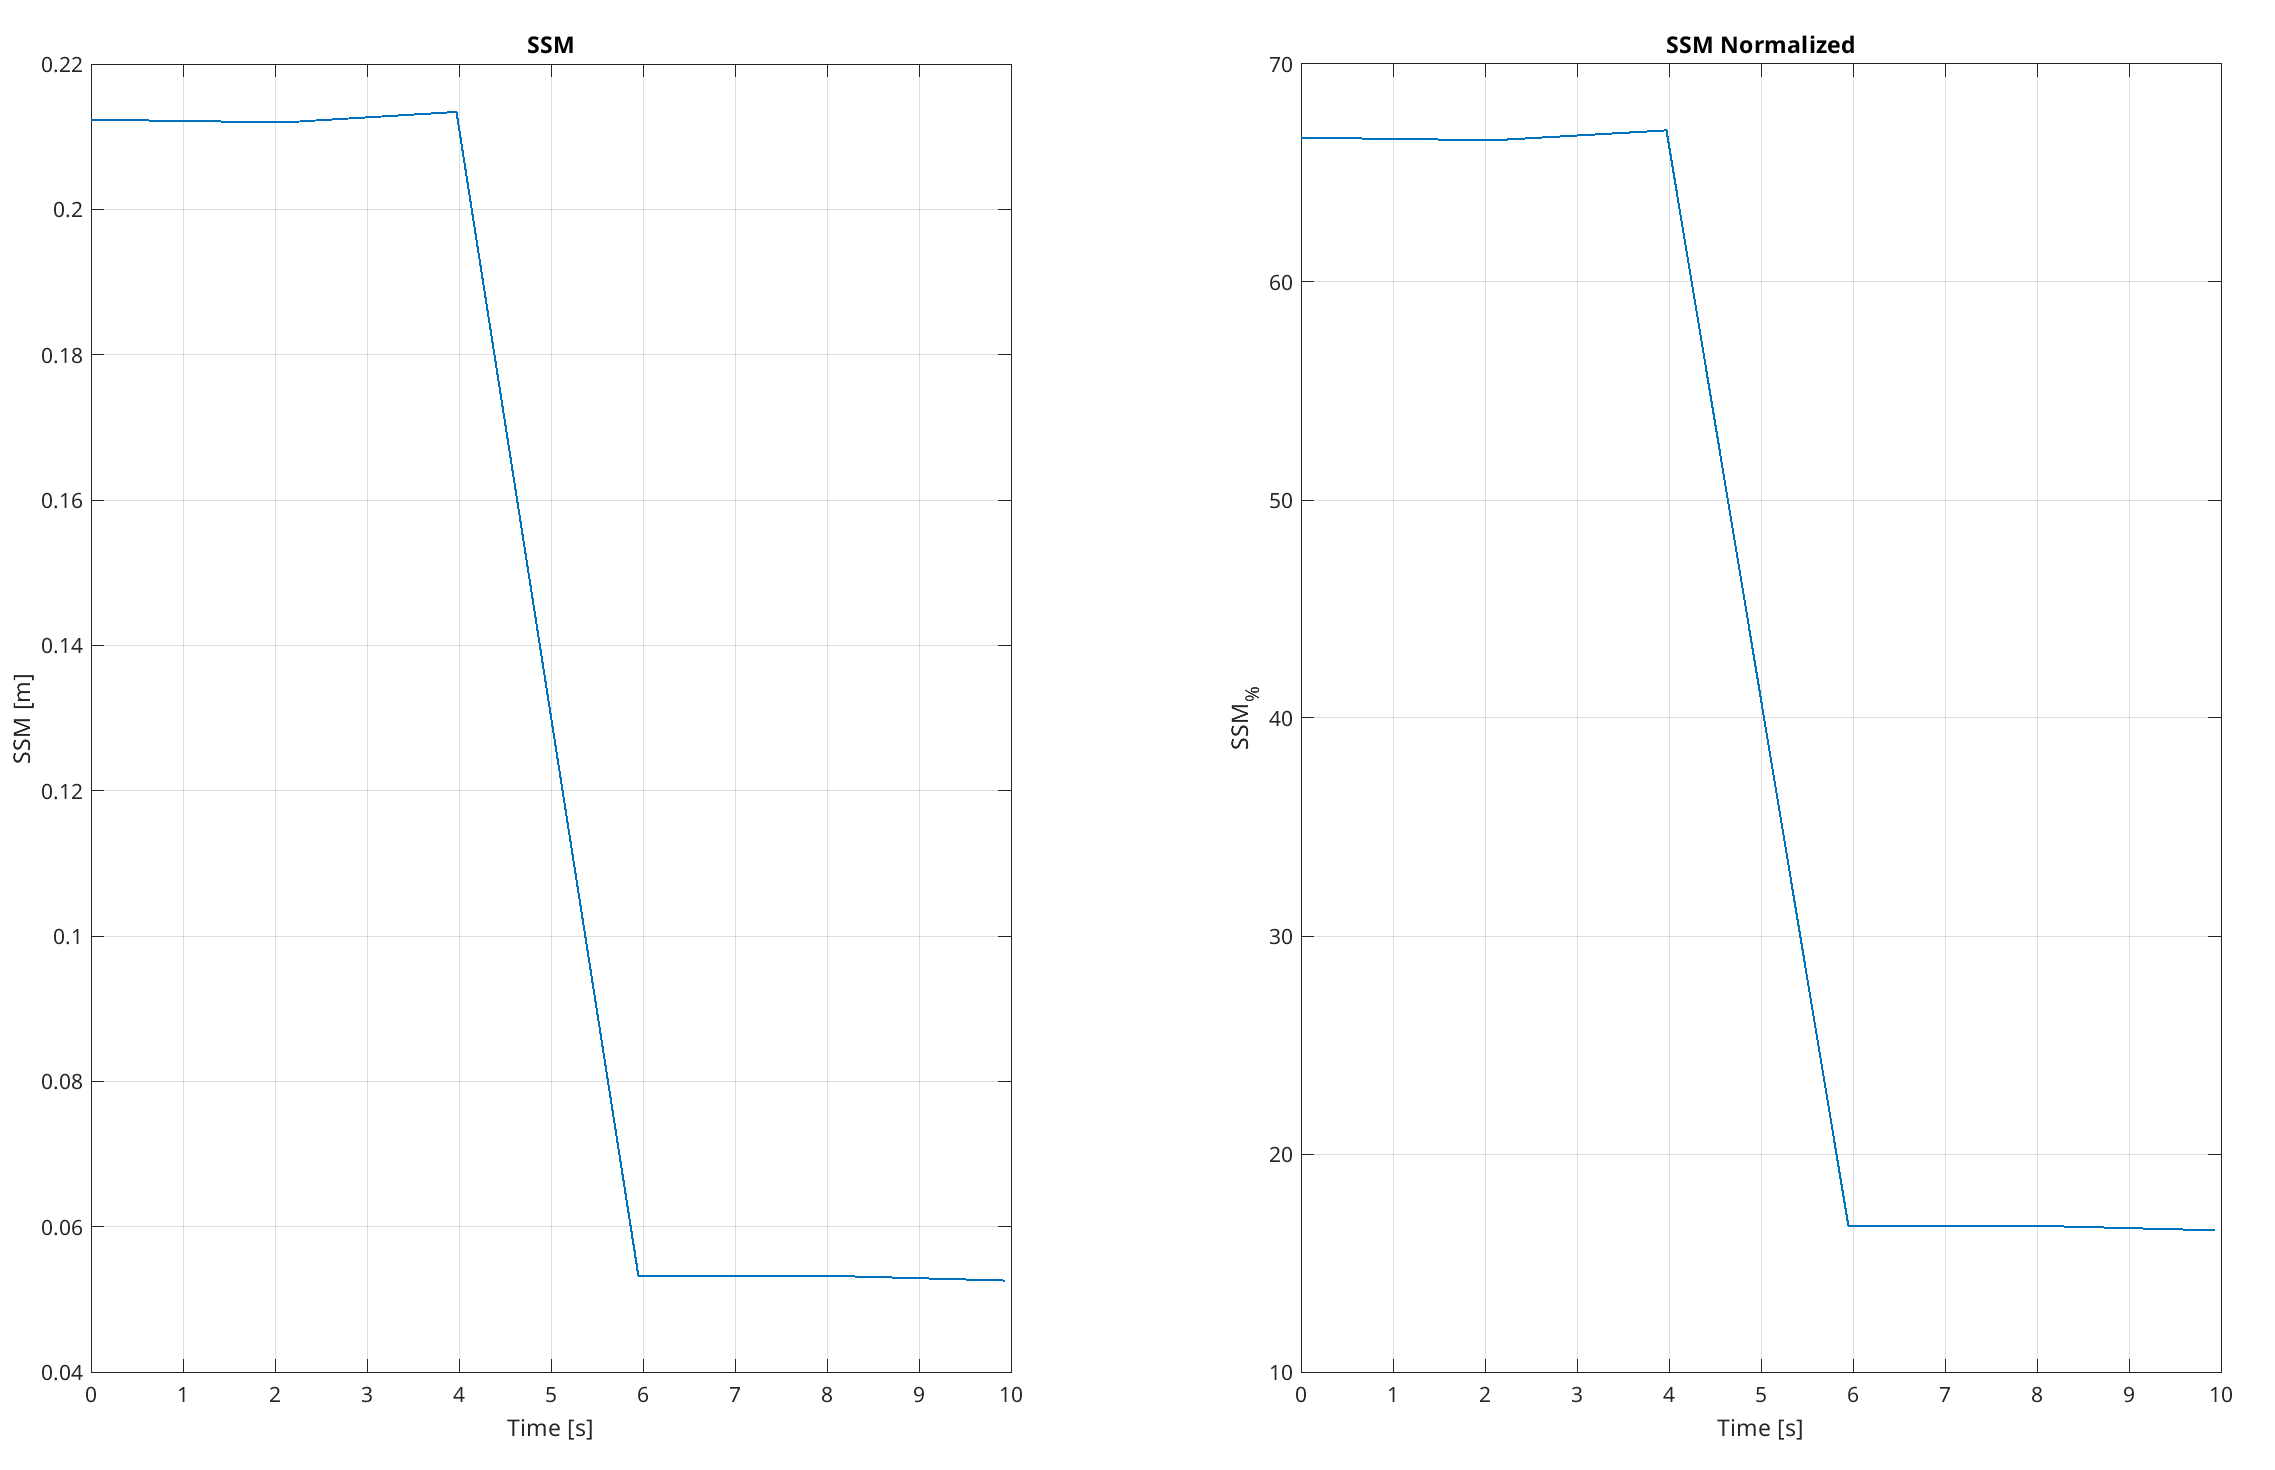
\includegraphics[width=0.9\textwidth]{Images/img_ch8/driving_SSM.png}
    \caption{SSM and $SSM_\%$, during driving test}
    \label{fig:driving_SSM_harmonic}
\end{figure}

%---- WHEEL TO GRIPPER ---- 
\subsection{Wheel to Gripper (W2G)}
\label{sec:gz_harmonic_W2G}

Here, the results of the driving-to-walking locomotion transformation are reported in the same order as the G2W above. 
First, some steps of the W2G algorithm execution in the simulator are shown in Fig.\ref{fig:W2G_harmonic}. The joint state tracking for each limb is represented in Figs.\ref{fig:W2G_LF_harmonic_joint} - \ref{fig:W2G_RF_harmonic_joint}, while the control torque from the IJCs in Figs.\ref{fig:W2G_LF_harmonic_torque} - \ref{fig:W2G_RF_harmonic_torque}.
Finally, the stability margins during the motion sequence are reported in Fig.\ref{fig:W2G_SSM_harmonic}.

\begin{figure}[H]
    \centering
    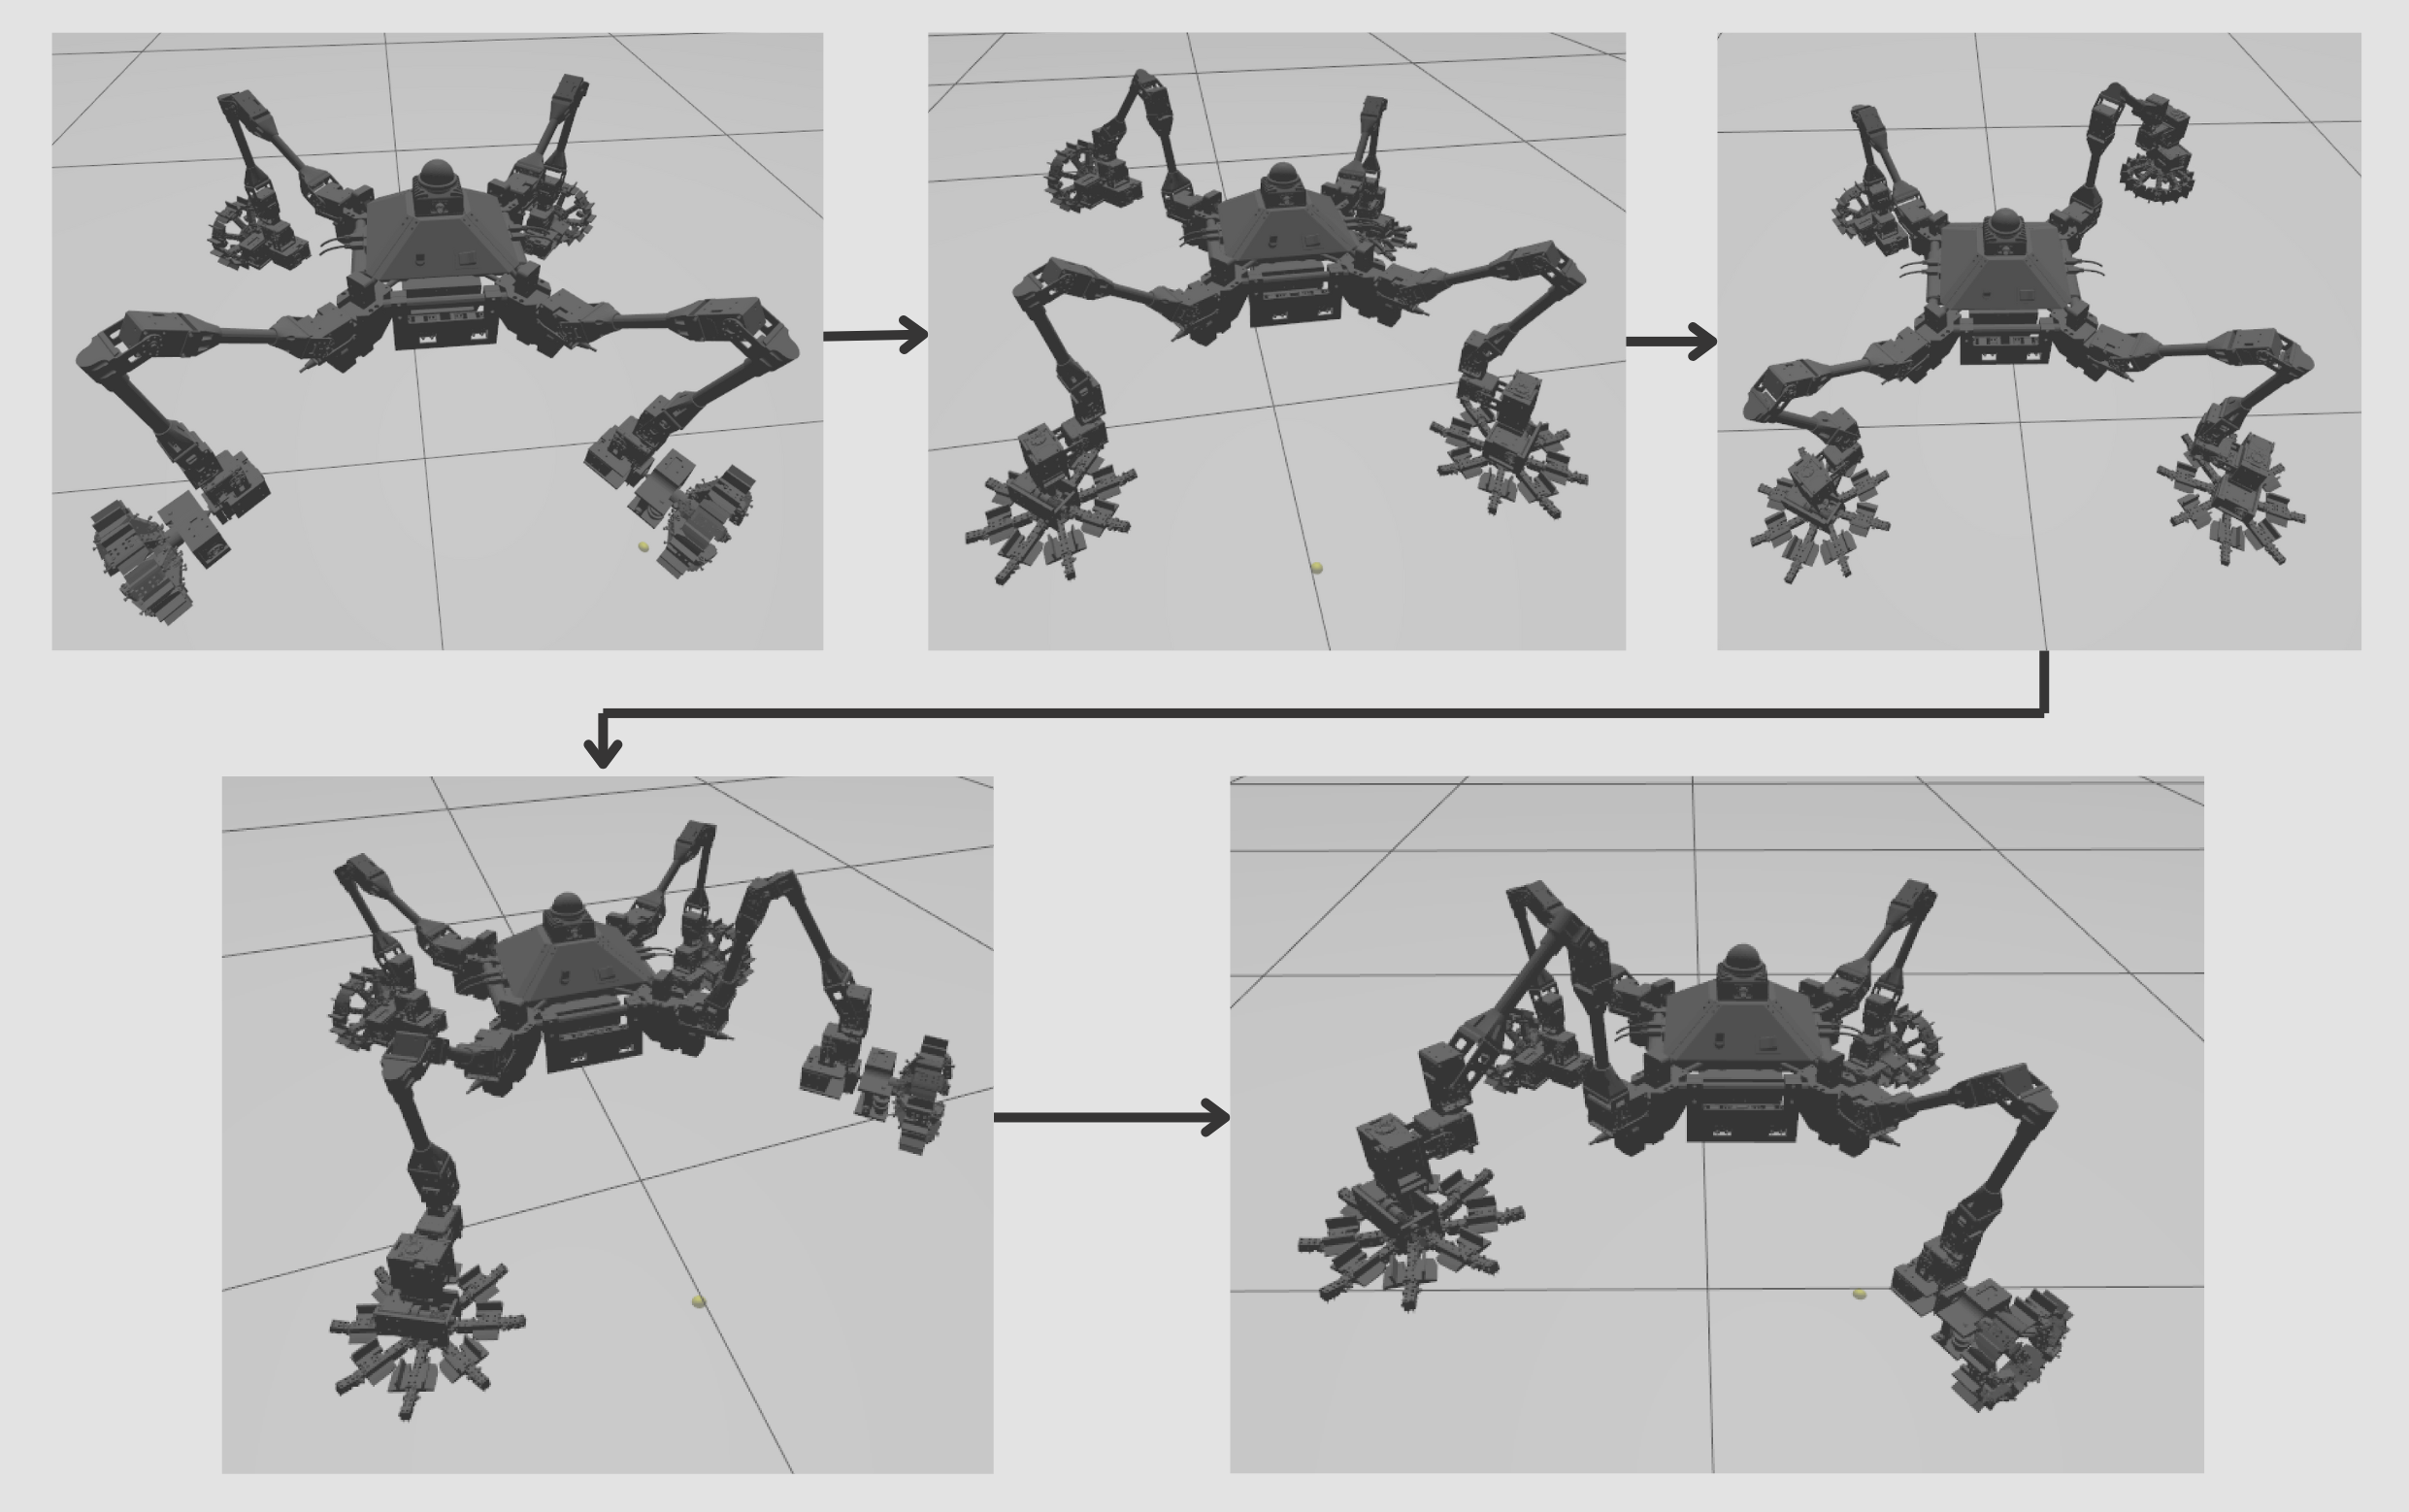
\includegraphics[width=0.9\textwidth]{Images/img_ch8/W2G_steps_sim.png}
    \caption{W2G Transition in Gazebo Harmonic}
    \label{fig:W2G_harmonic}
\end{figure}

\begin{figure}[H]
    \centering
    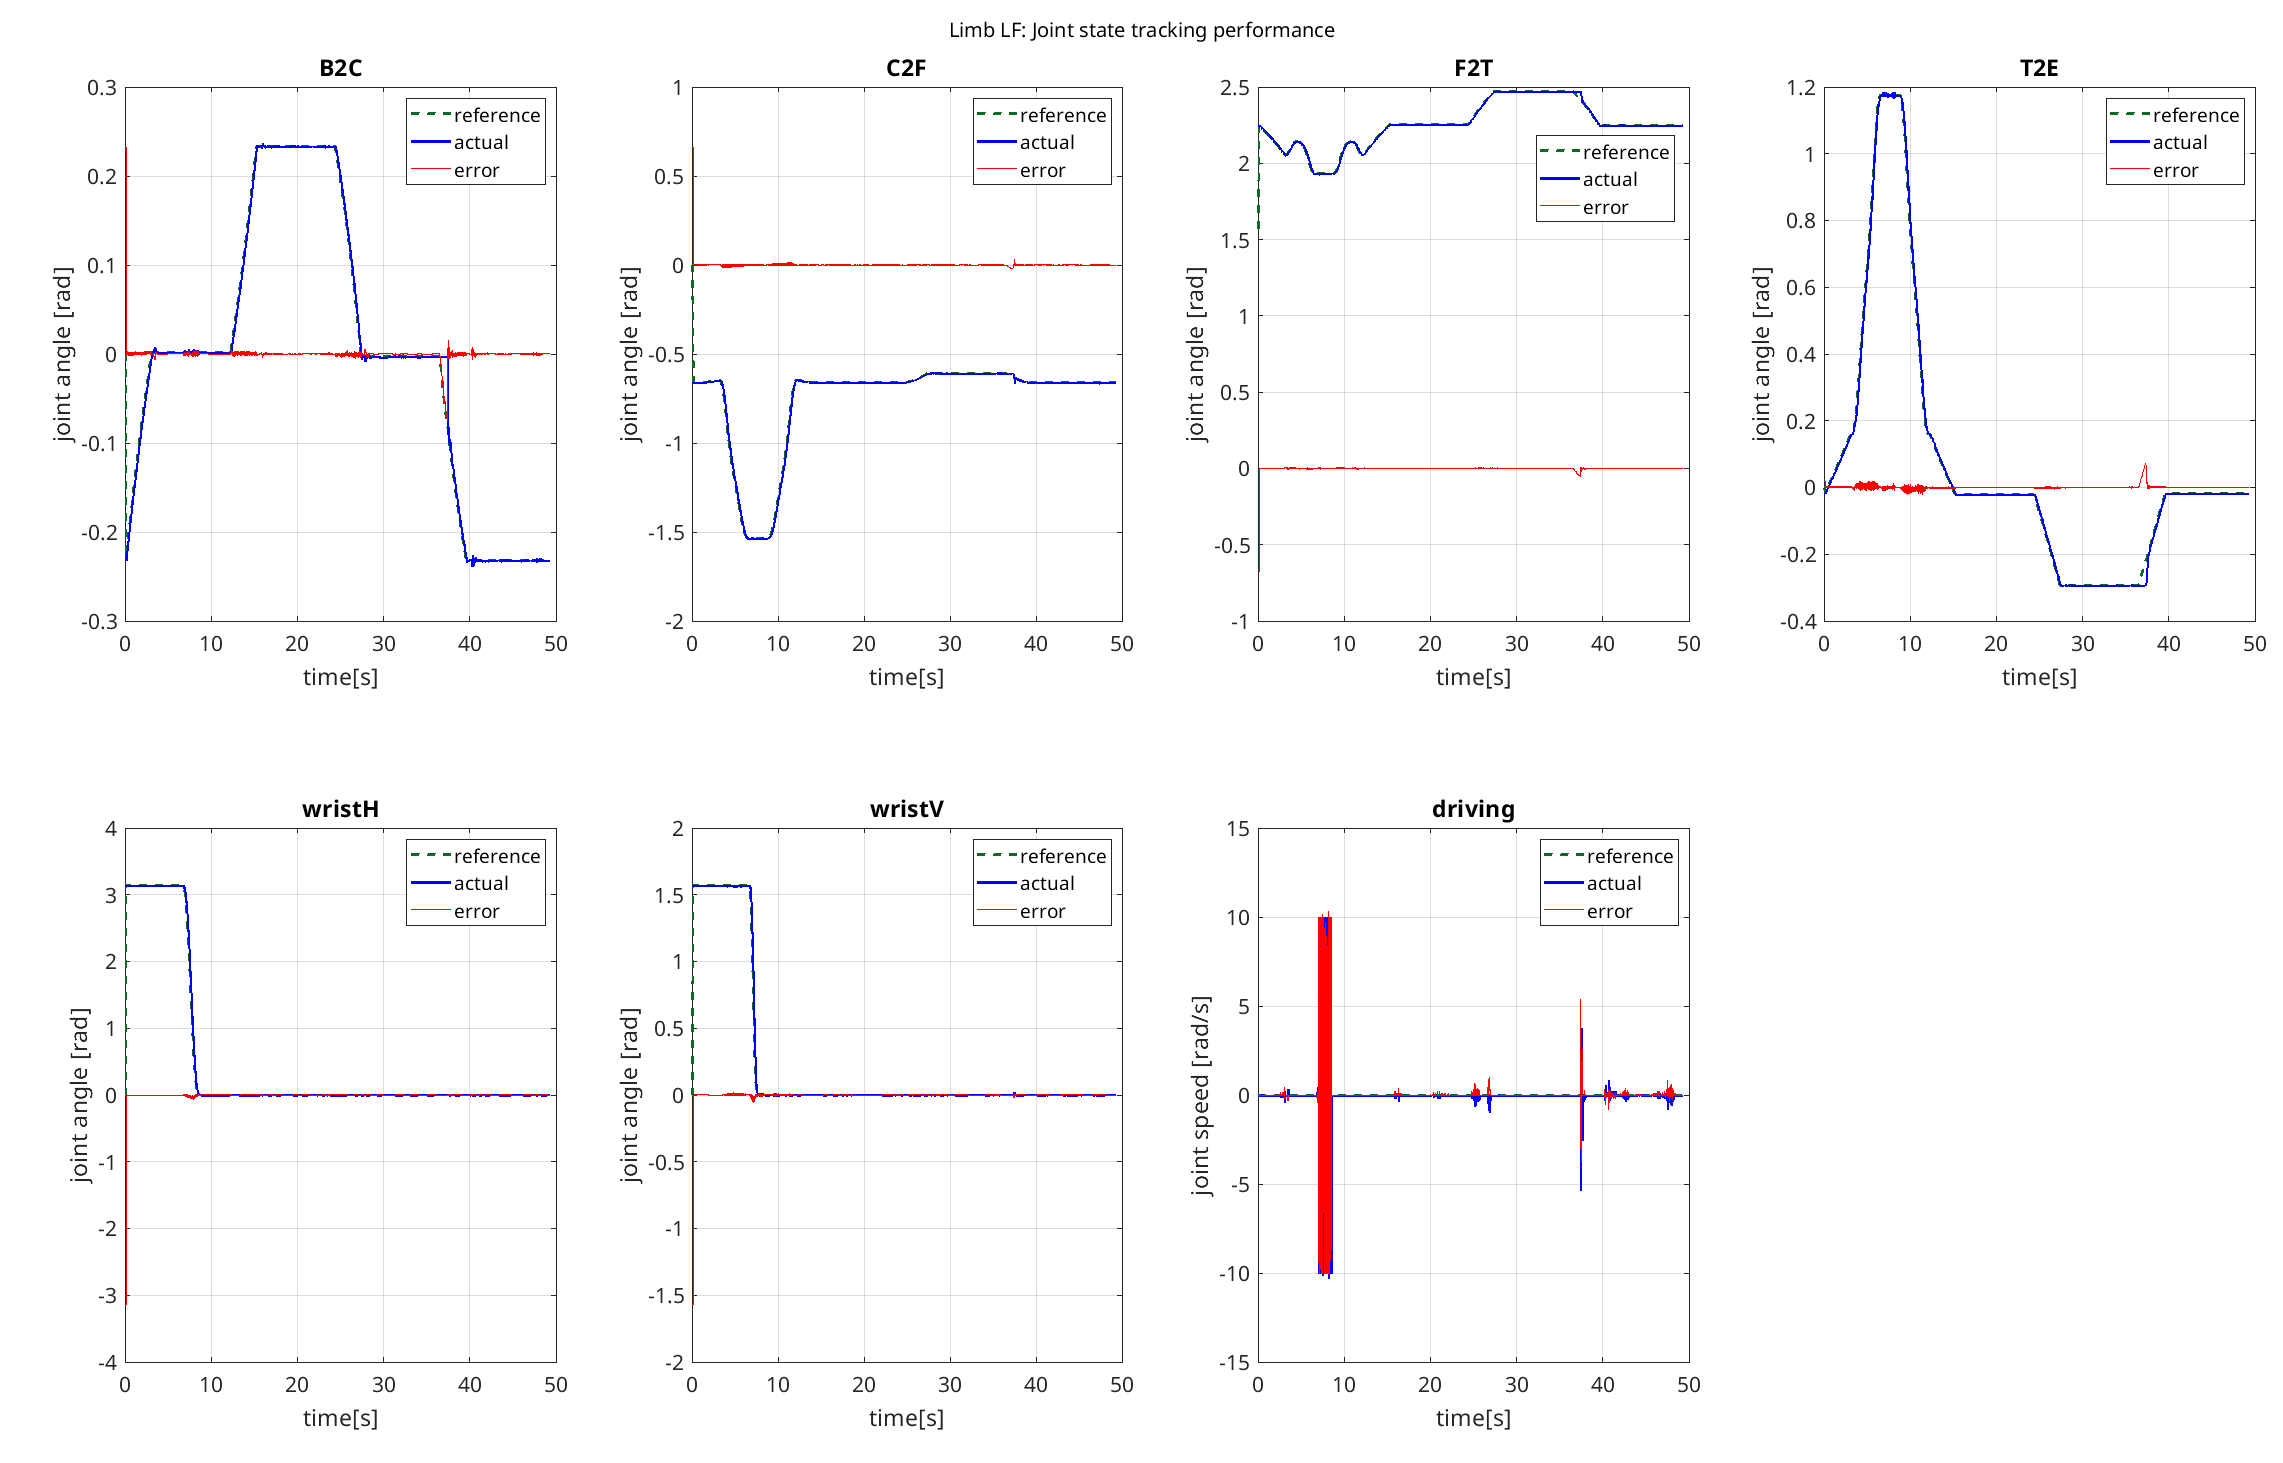
\includegraphics[width=1.0\textwidth]{Images/img_ch8/W2G_LF_joints.png}
    \caption{LF limb, Joint tracking during W2G}
    \label{fig:W2G_LF_harmonic_joint}
\end{figure}

\begin{figure}[H]
    \centering
    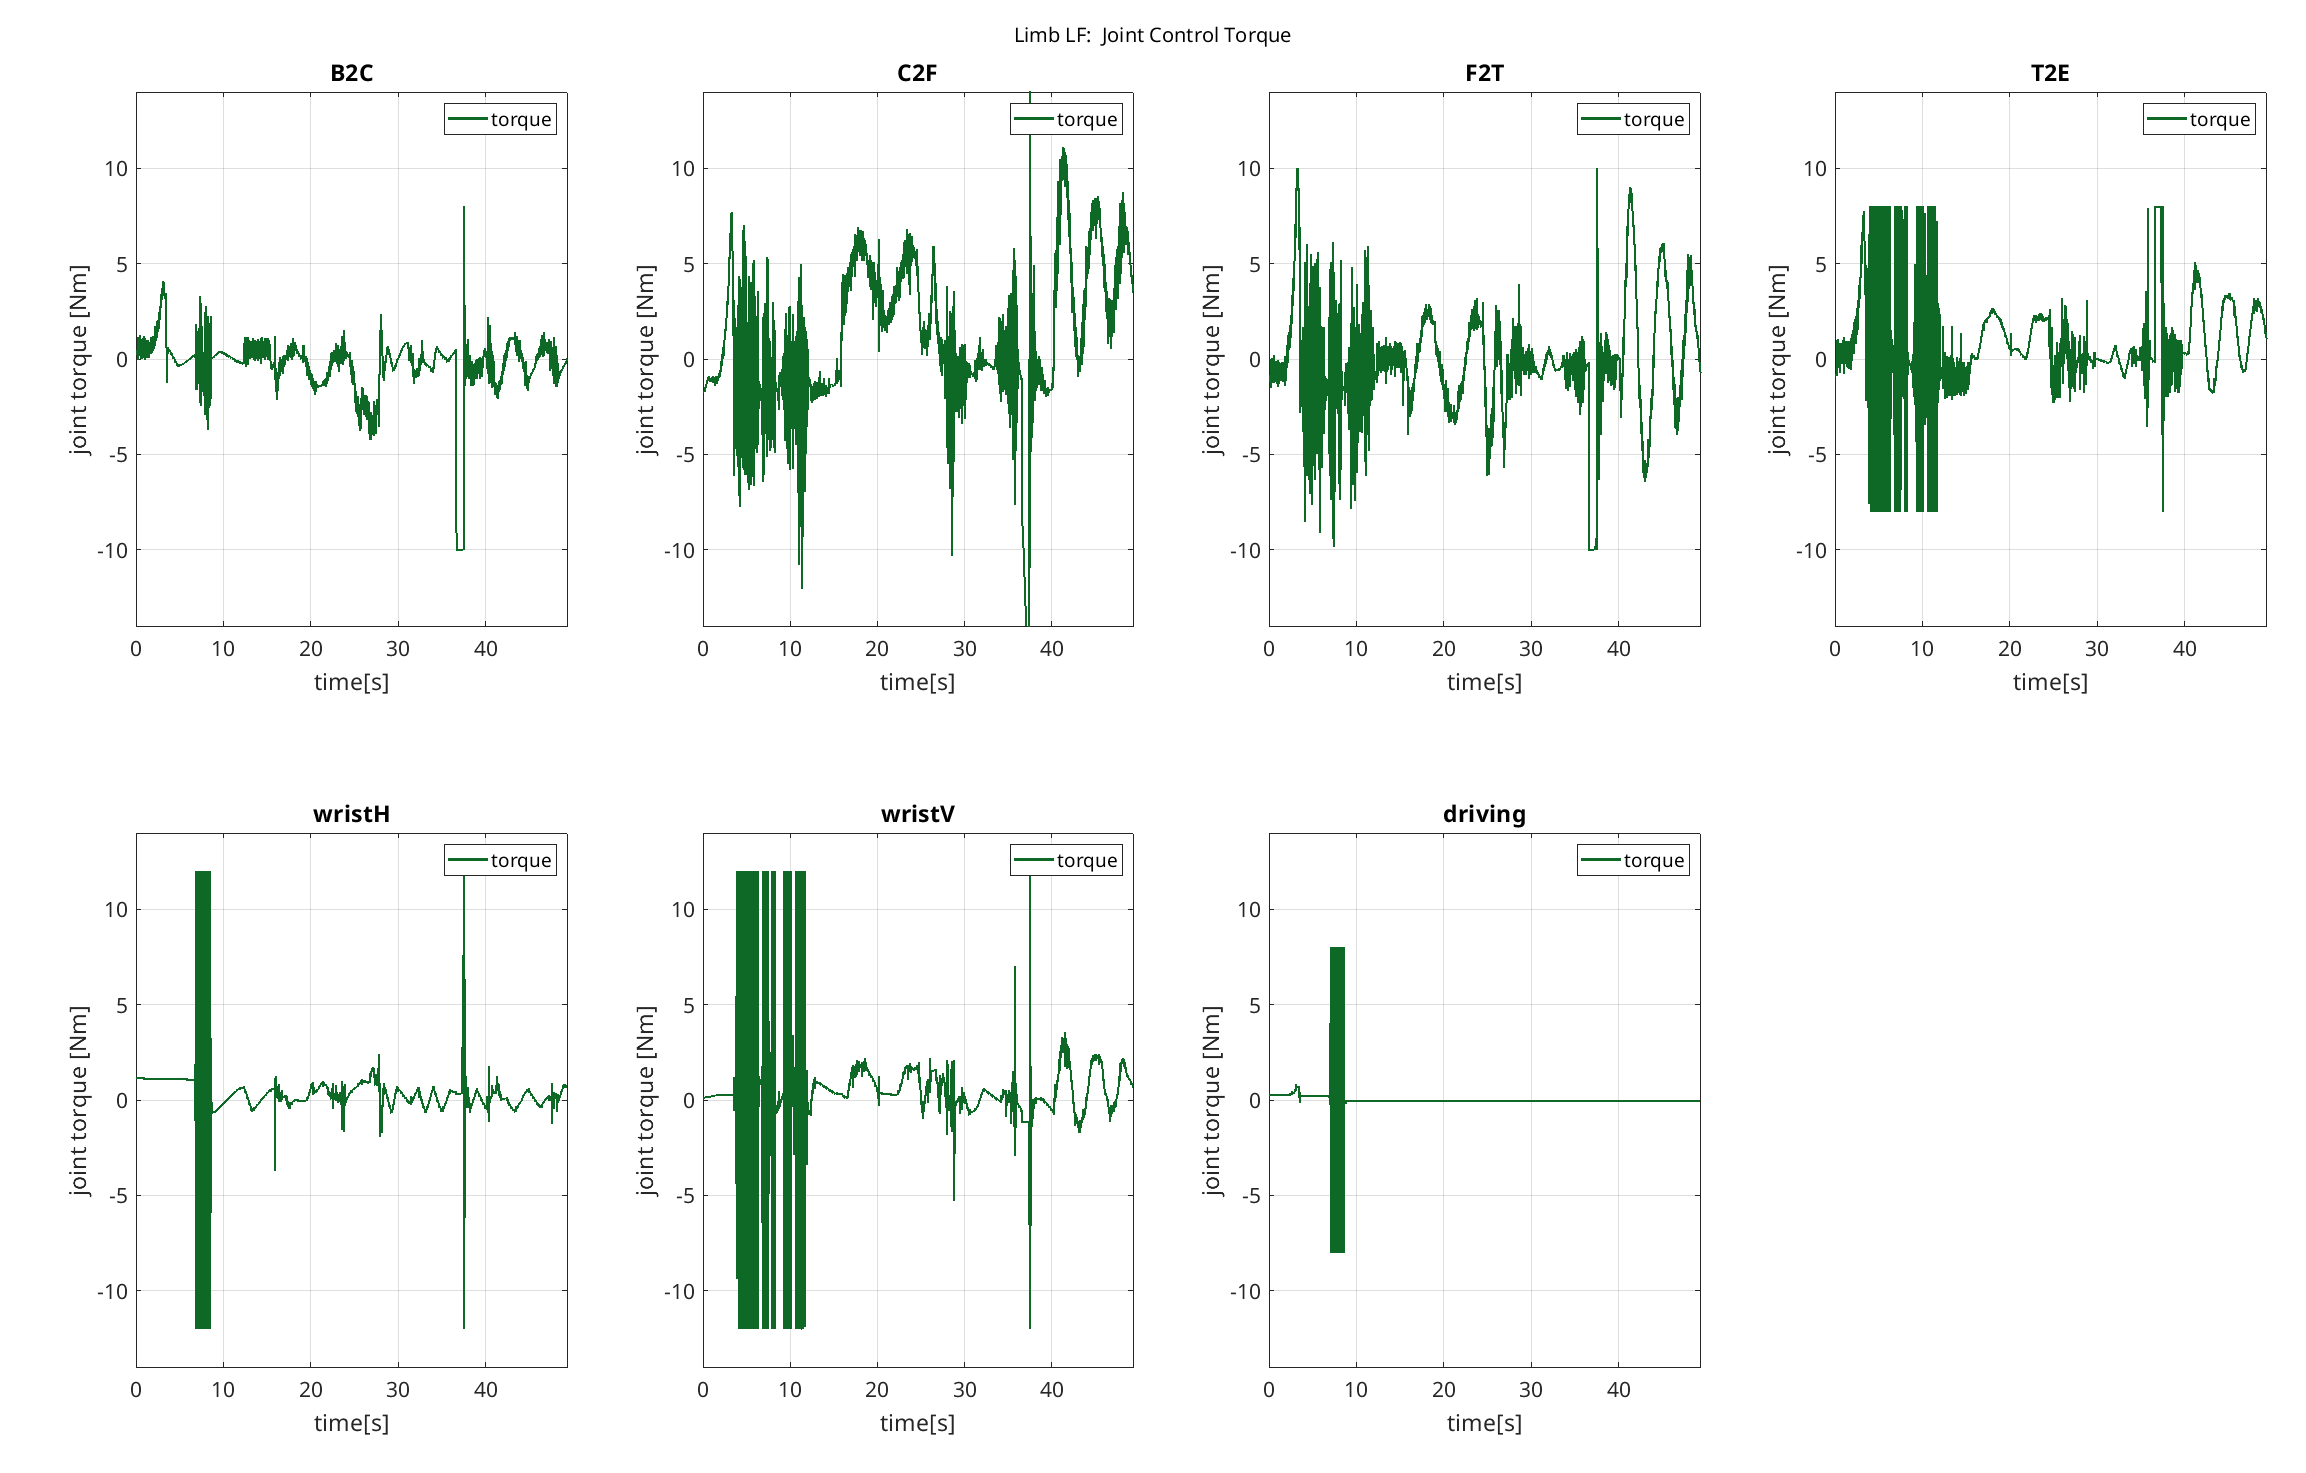
\includegraphics[width=1.0\textwidth]{Images/img_ch8/W2G_LF_torque.png}
    \caption{LF limb, Joint torques during W2G}
    \label{fig:W2G_LF_harmonic_torque}
\end{figure}

\begin{figure}[H]
    \centering
    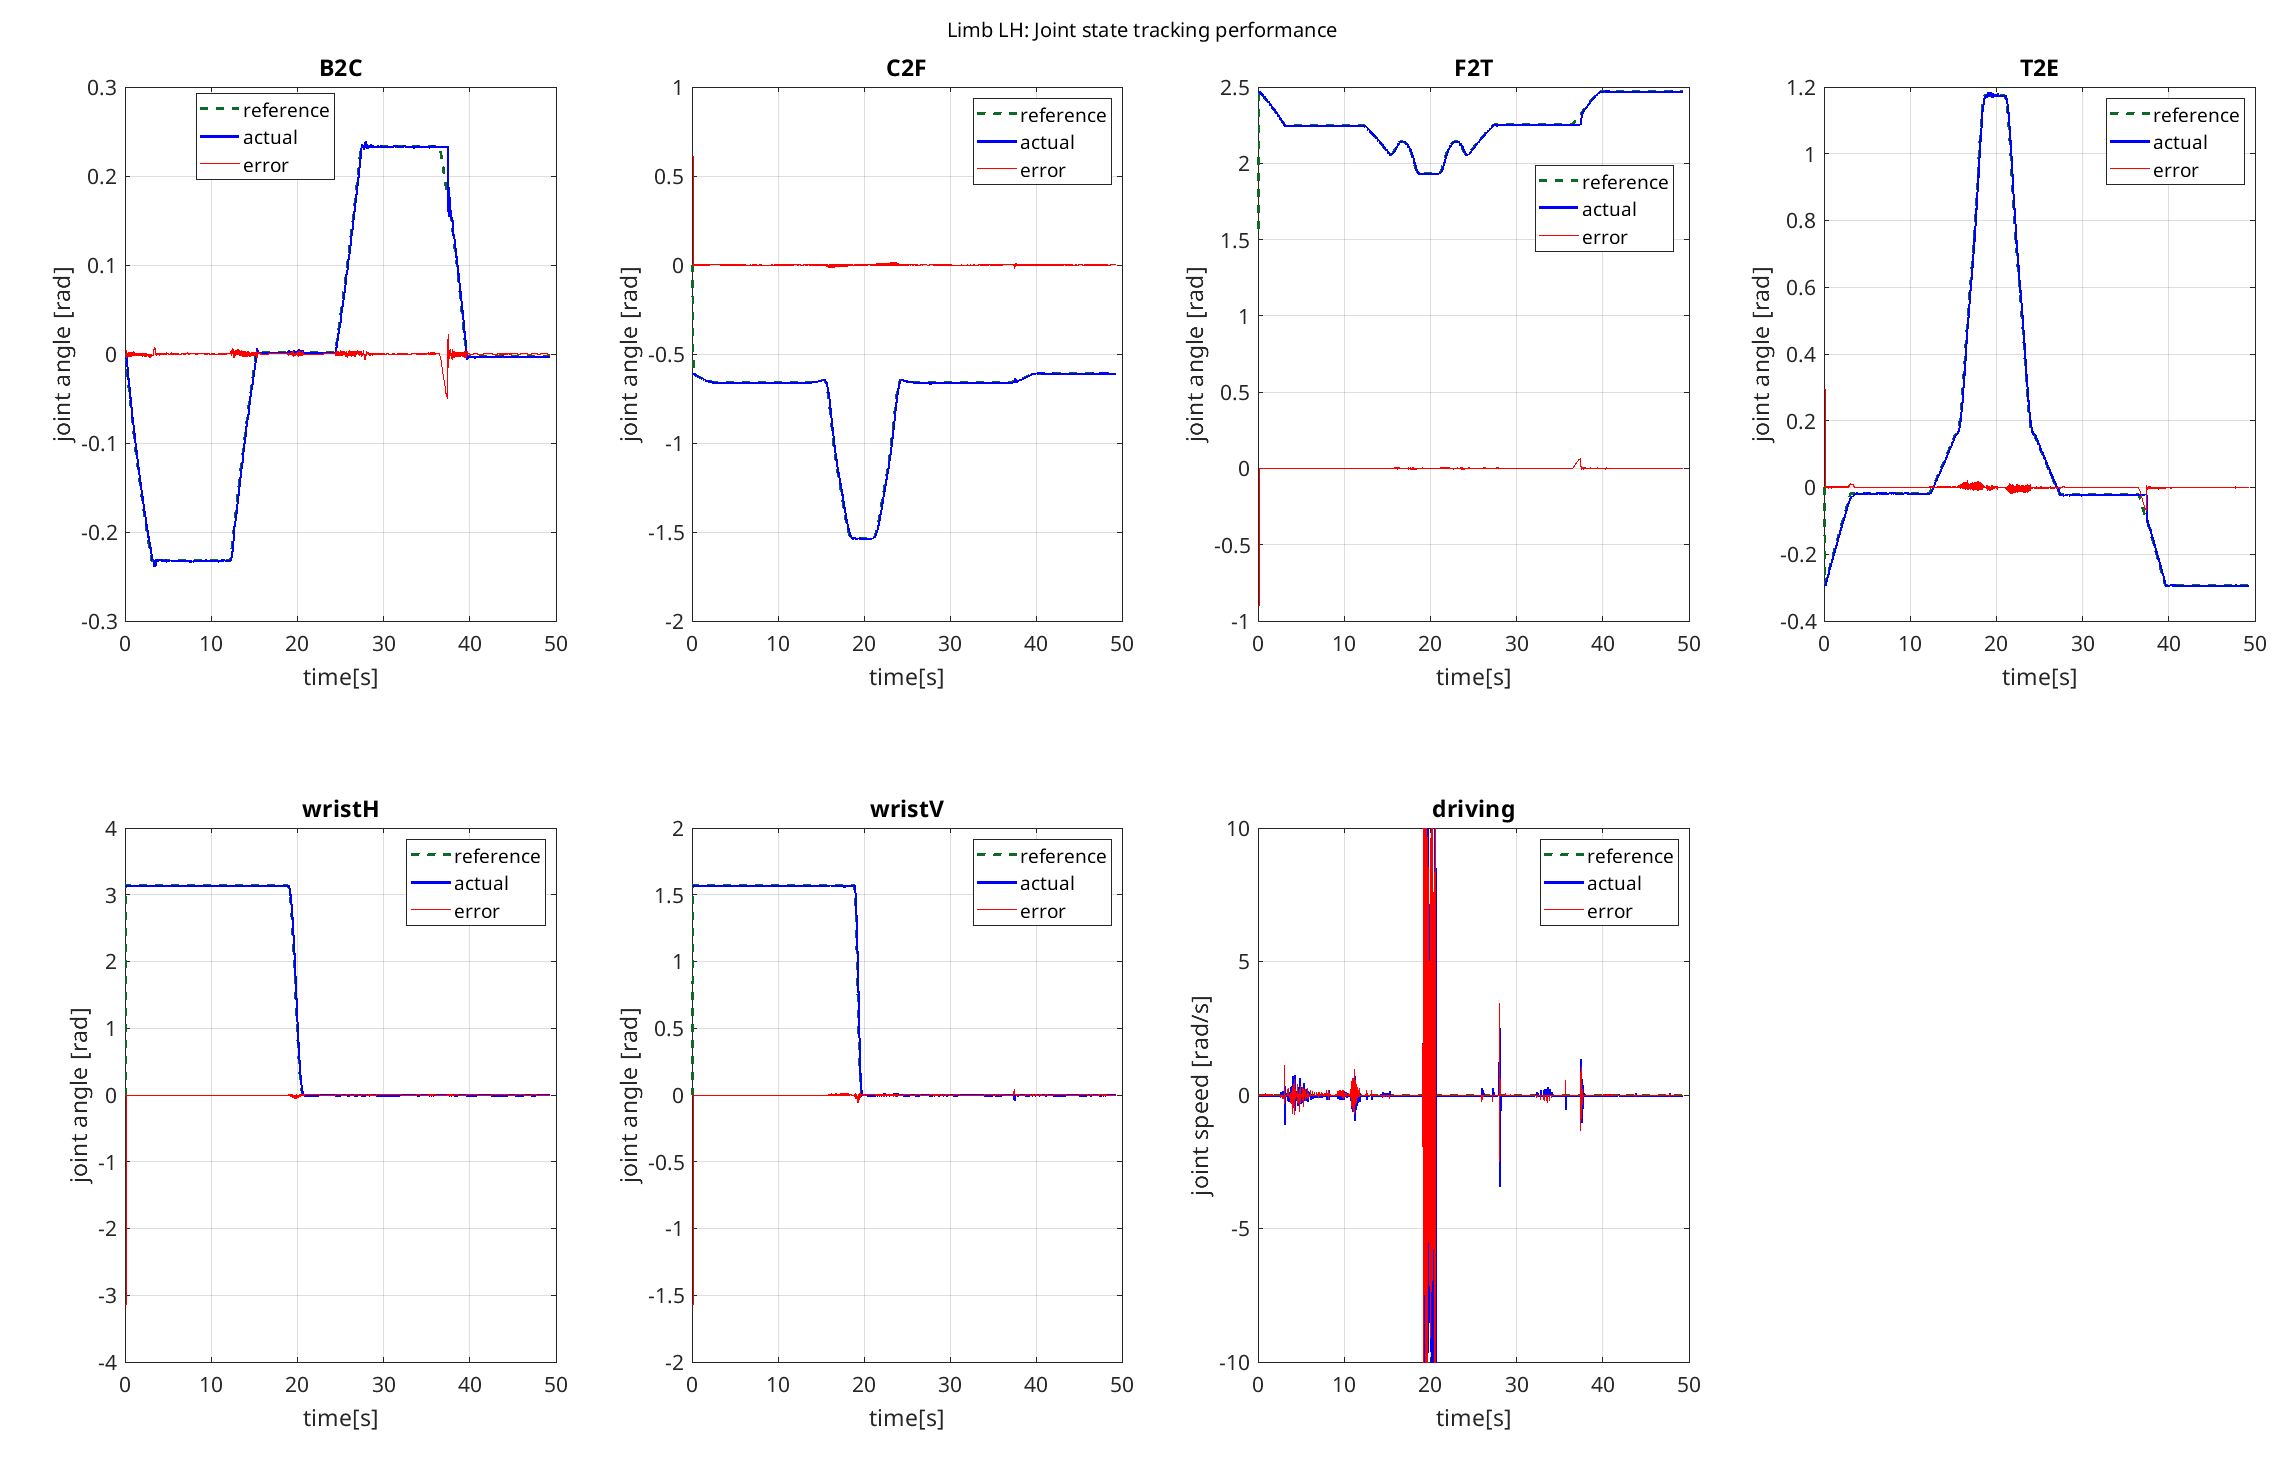
\includegraphics[width=1.0\textwidth]{Images/img_ch8/W2G_LH_joints.png}
    \caption{LH limb, Joint tracking during W2G}
    \label{fig:W2G_LH_harmonic_joint}
\end{figure}

\begin{figure}[H]
    \centering
    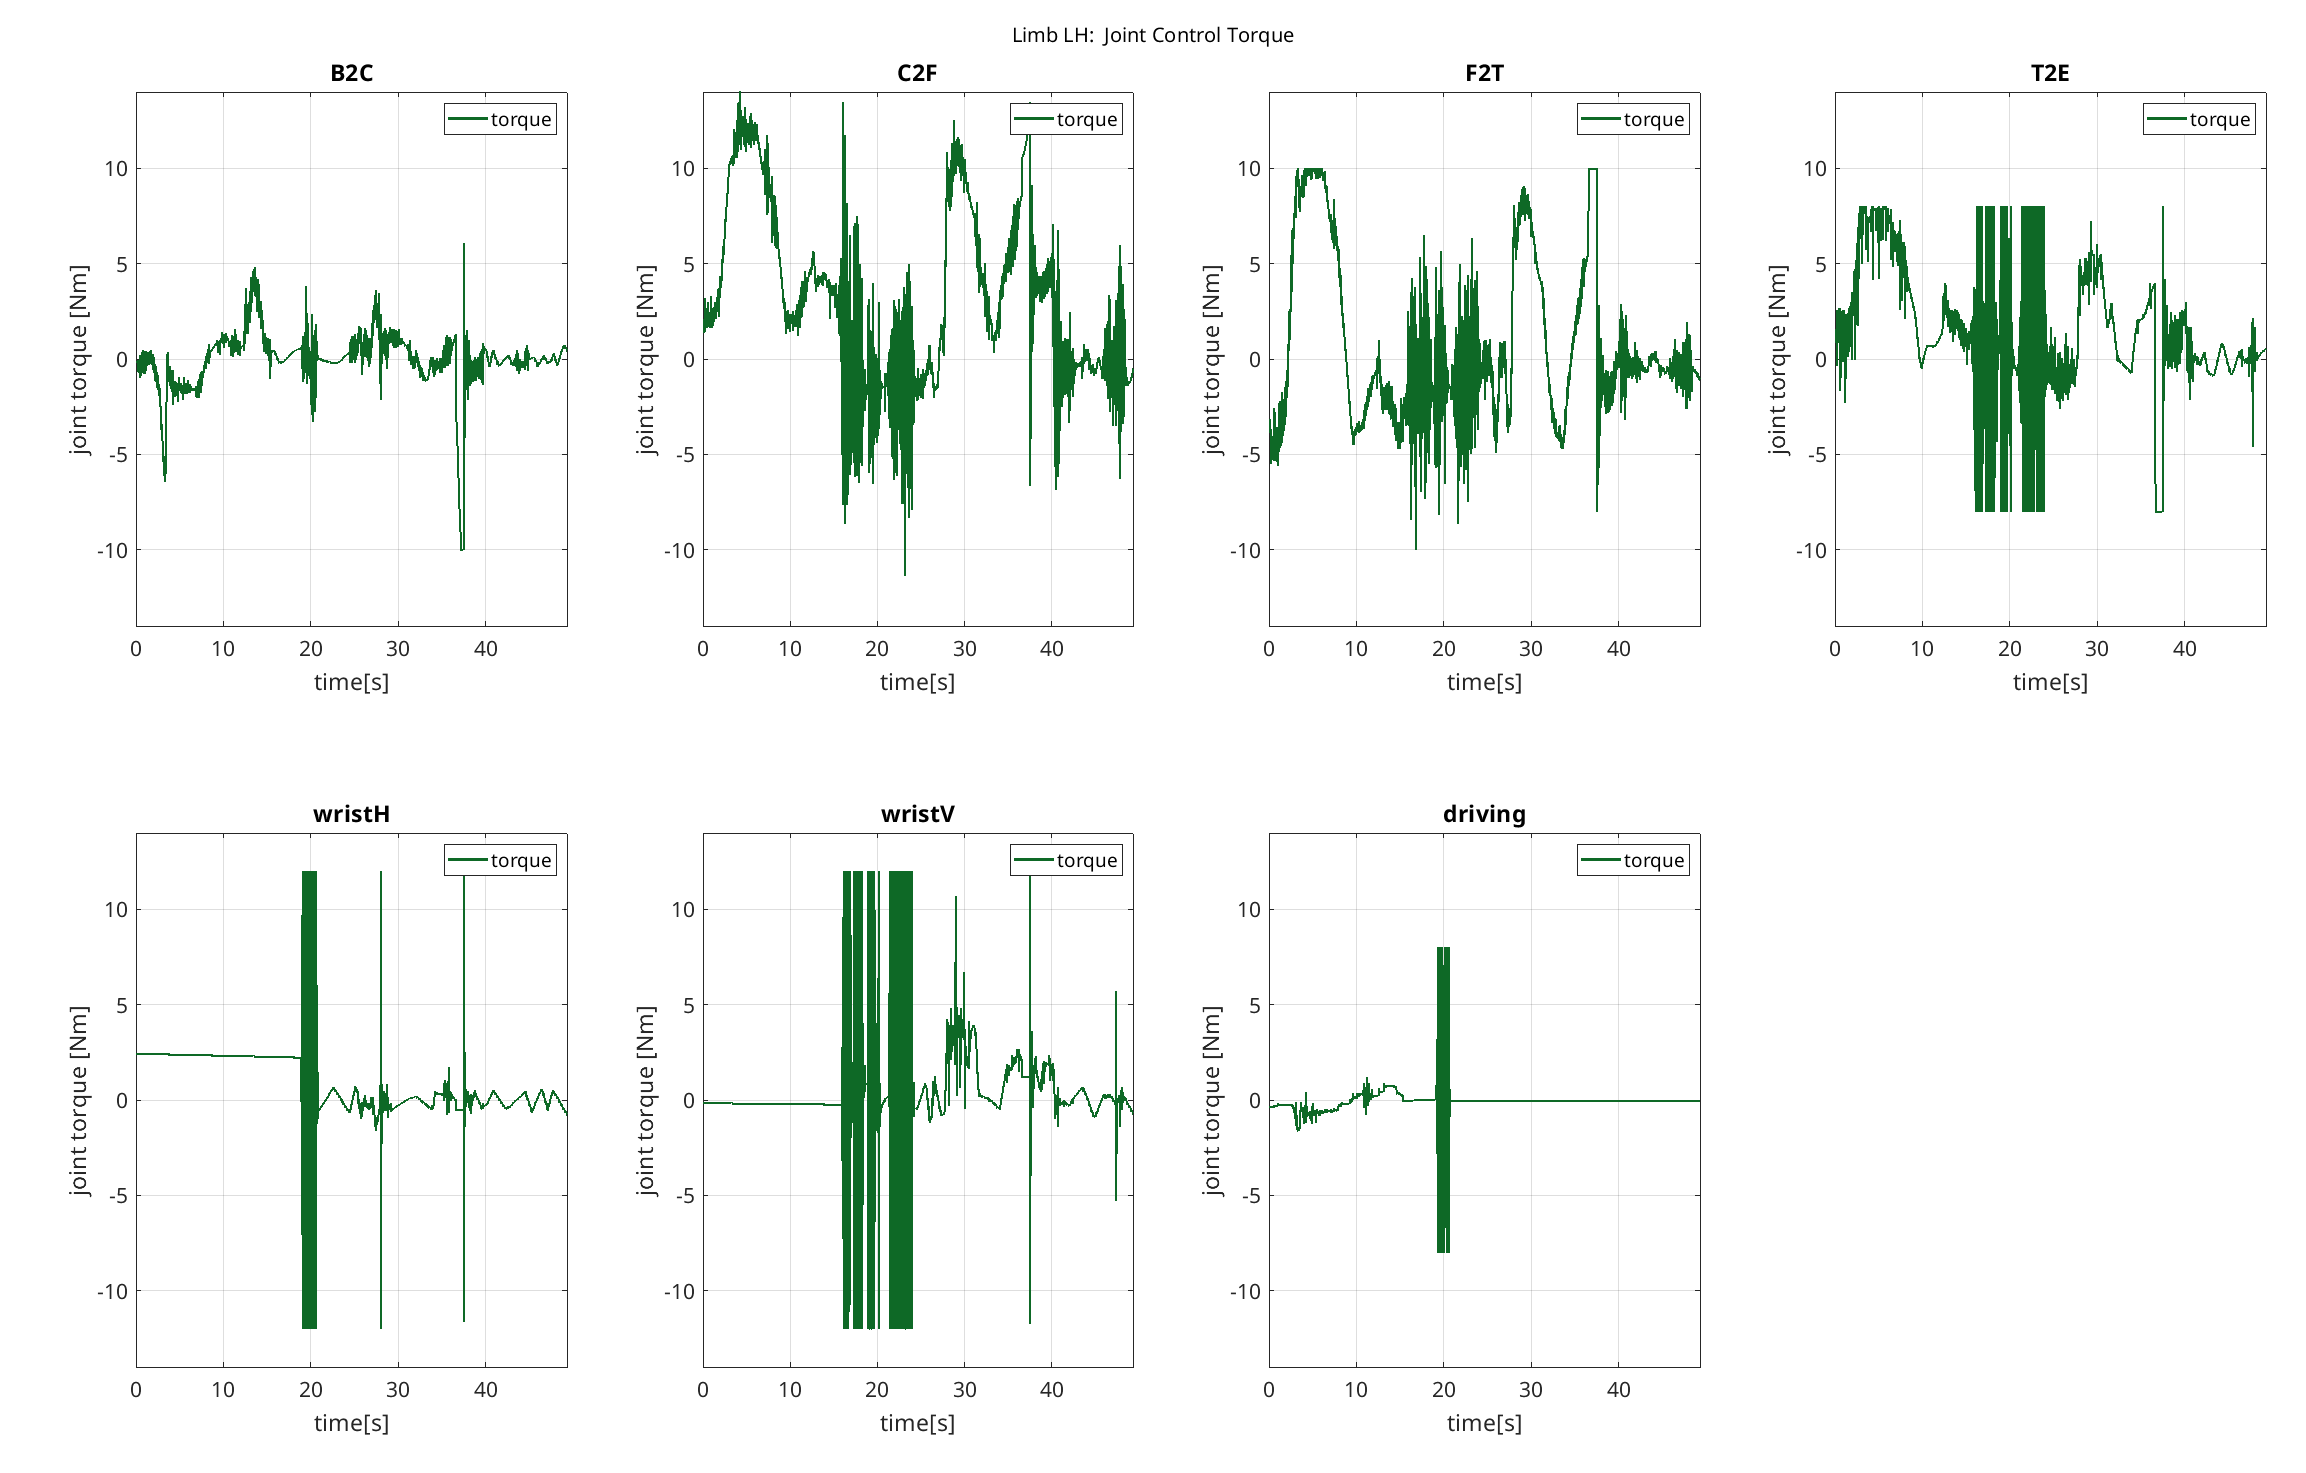
\includegraphics[width=1.0\textwidth]{Images/img_ch8/W2G_LH_torque.png}
    \caption{LH limb, Joint torques during W2G}
    \label{fig:W2G_LF_harmonic_torque}
\end{figure}
\begin{figure}[H]
    \centering
    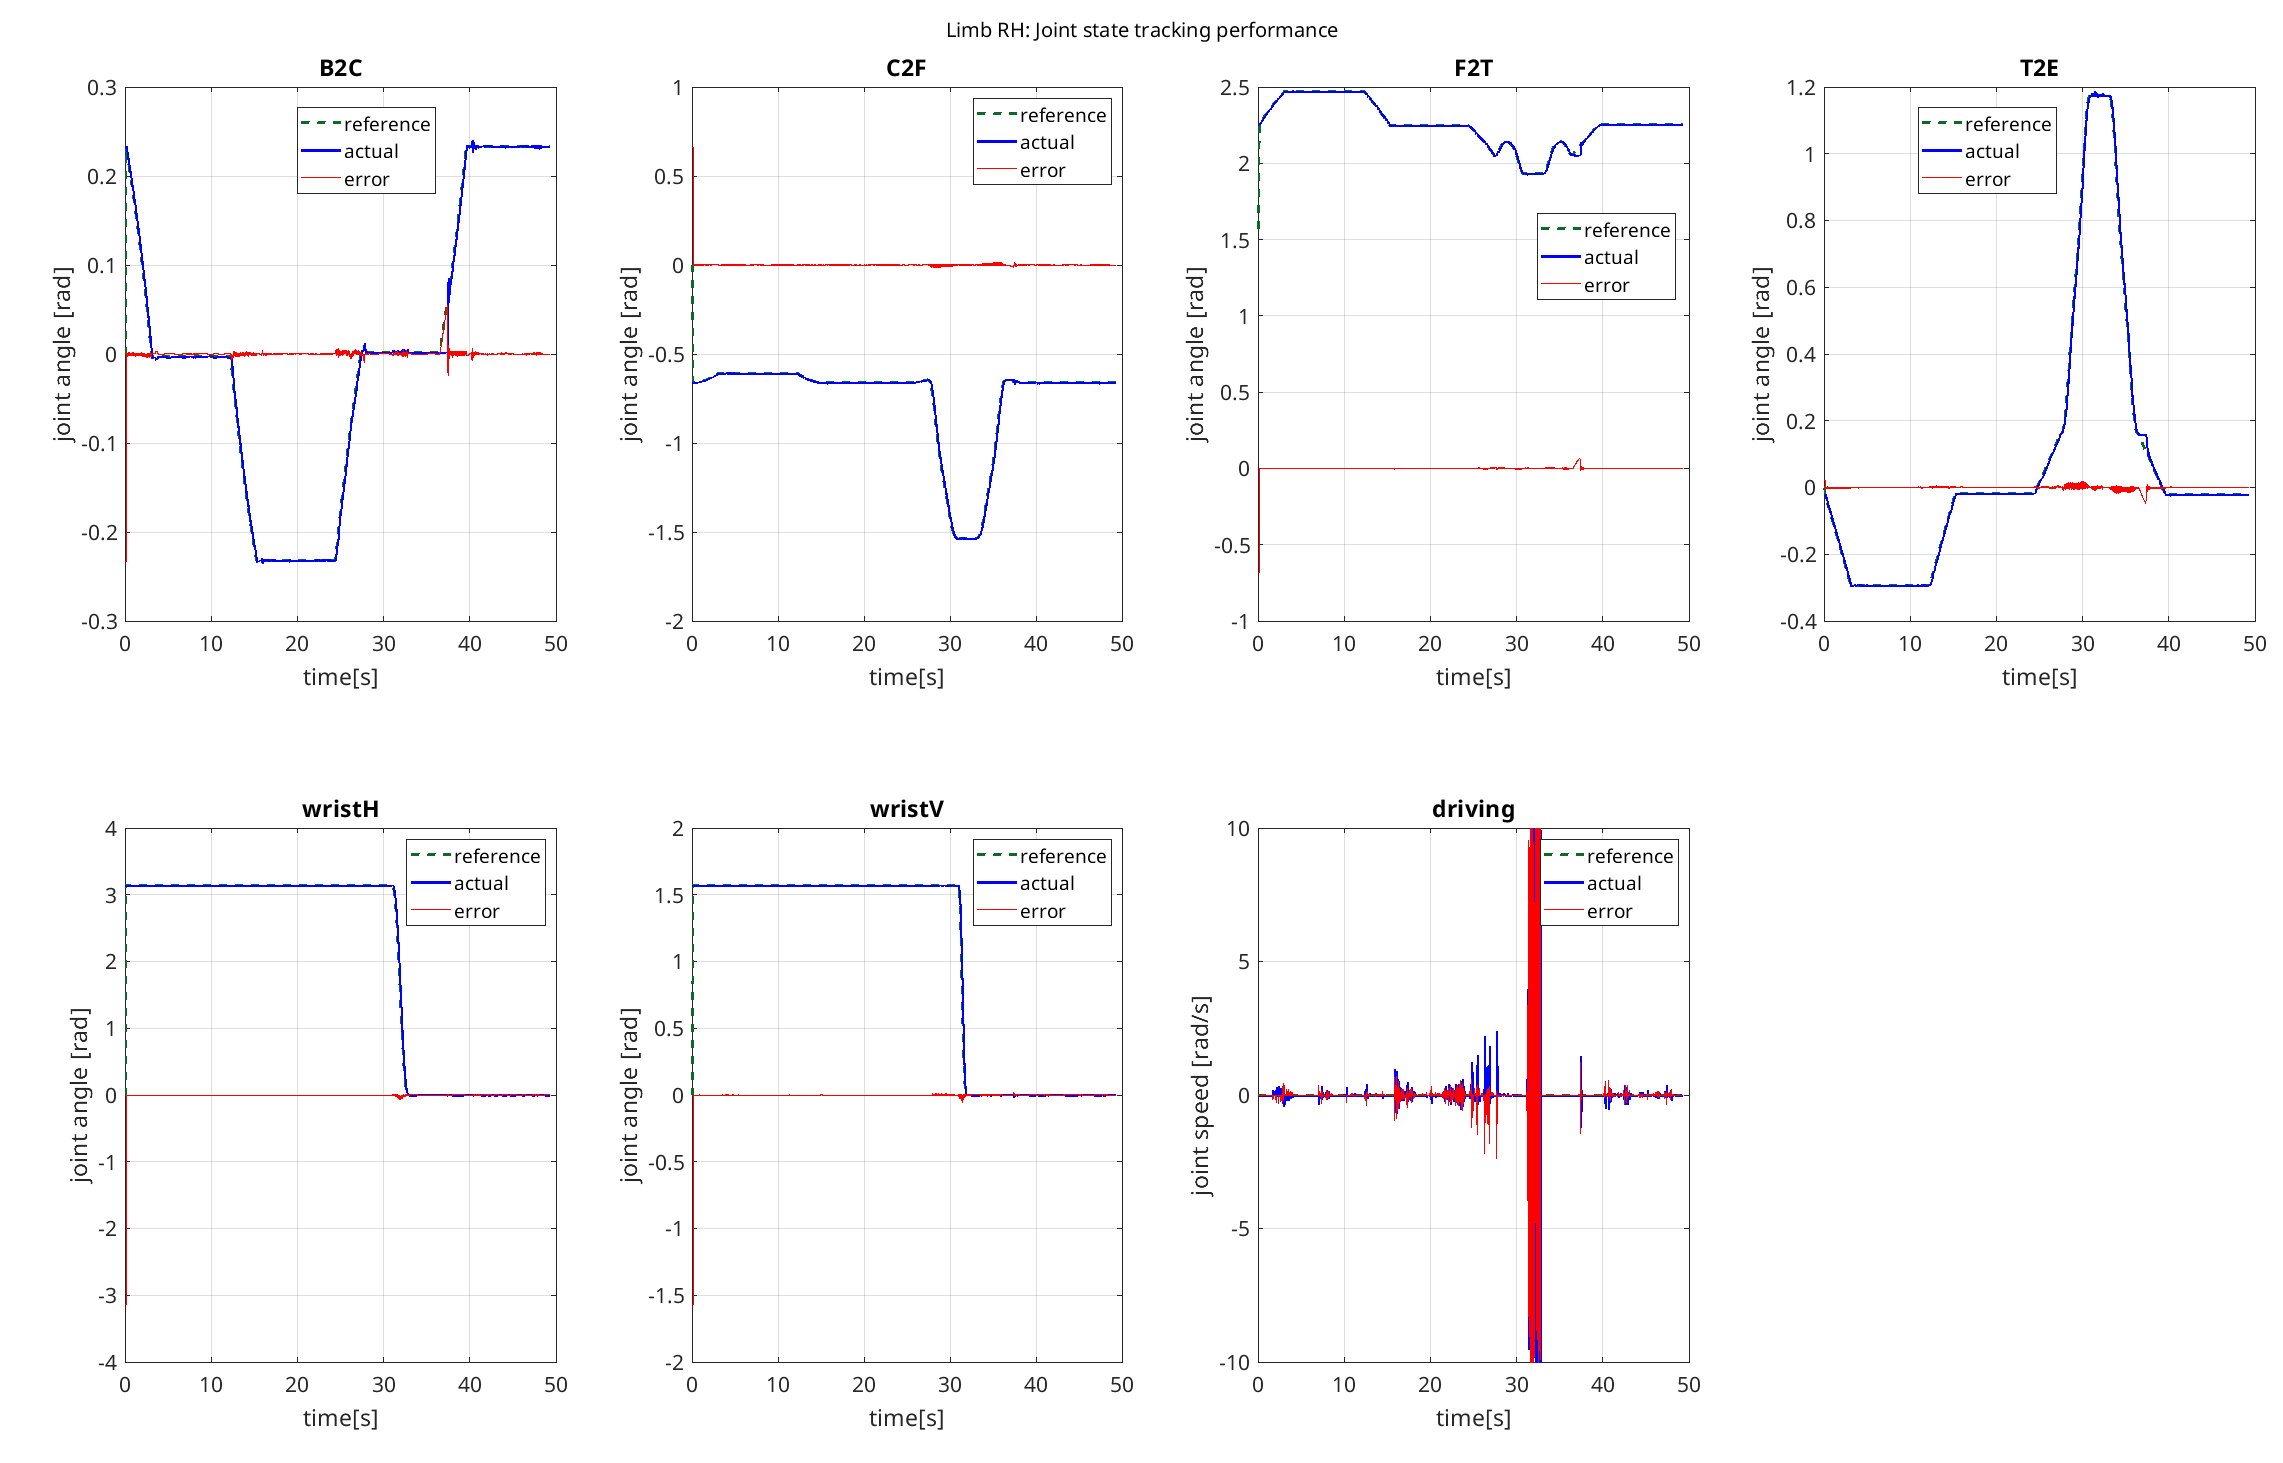
\includegraphics[width=1.0\textwidth]{Images/img_ch8/W2G_RH_joints.png}
    \caption{RH limb, Joint tracking during W2G}
    \label{fig:W2G_RH_harmonic_joint}
\end{figure}

\begin{figure}[H]
    \centering
    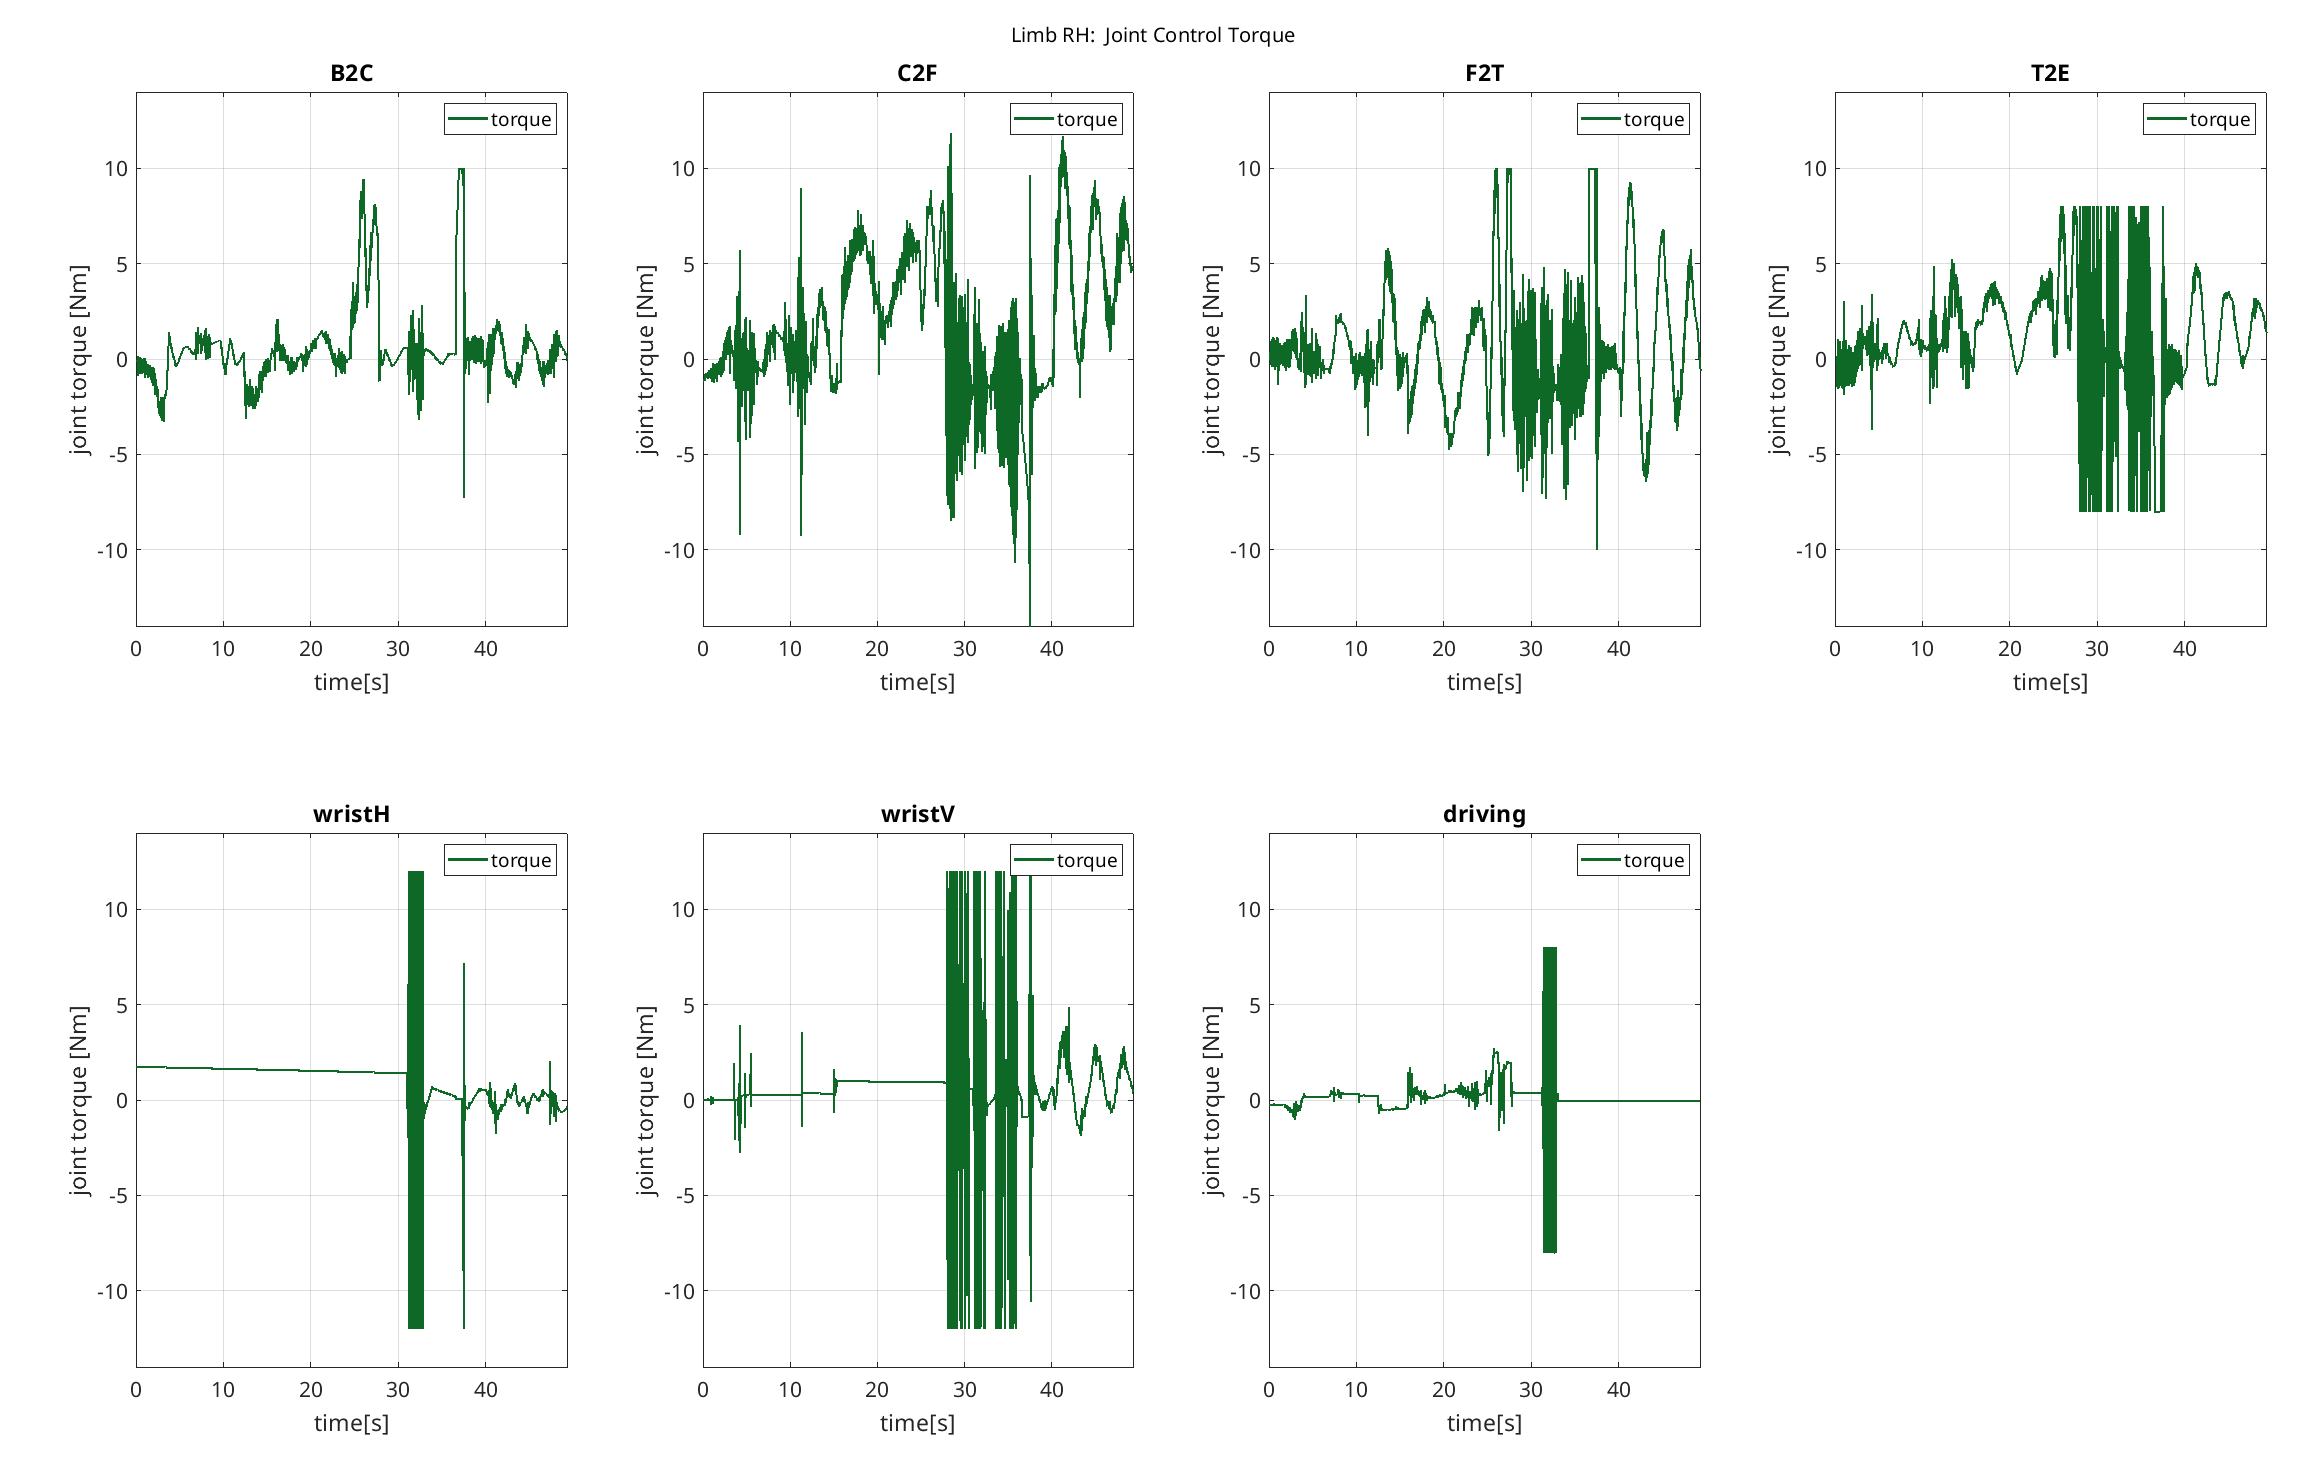
\includegraphics[width=1.0\textwidth]{Images/img_ch8/W2G_RH_torque.png}
    \caption{RH limb, Joint torques during W2G}
    \label{fig:W2G_RH_harmonic_torque}
\end{figure}

\begin{figure}[H]
    \centering
    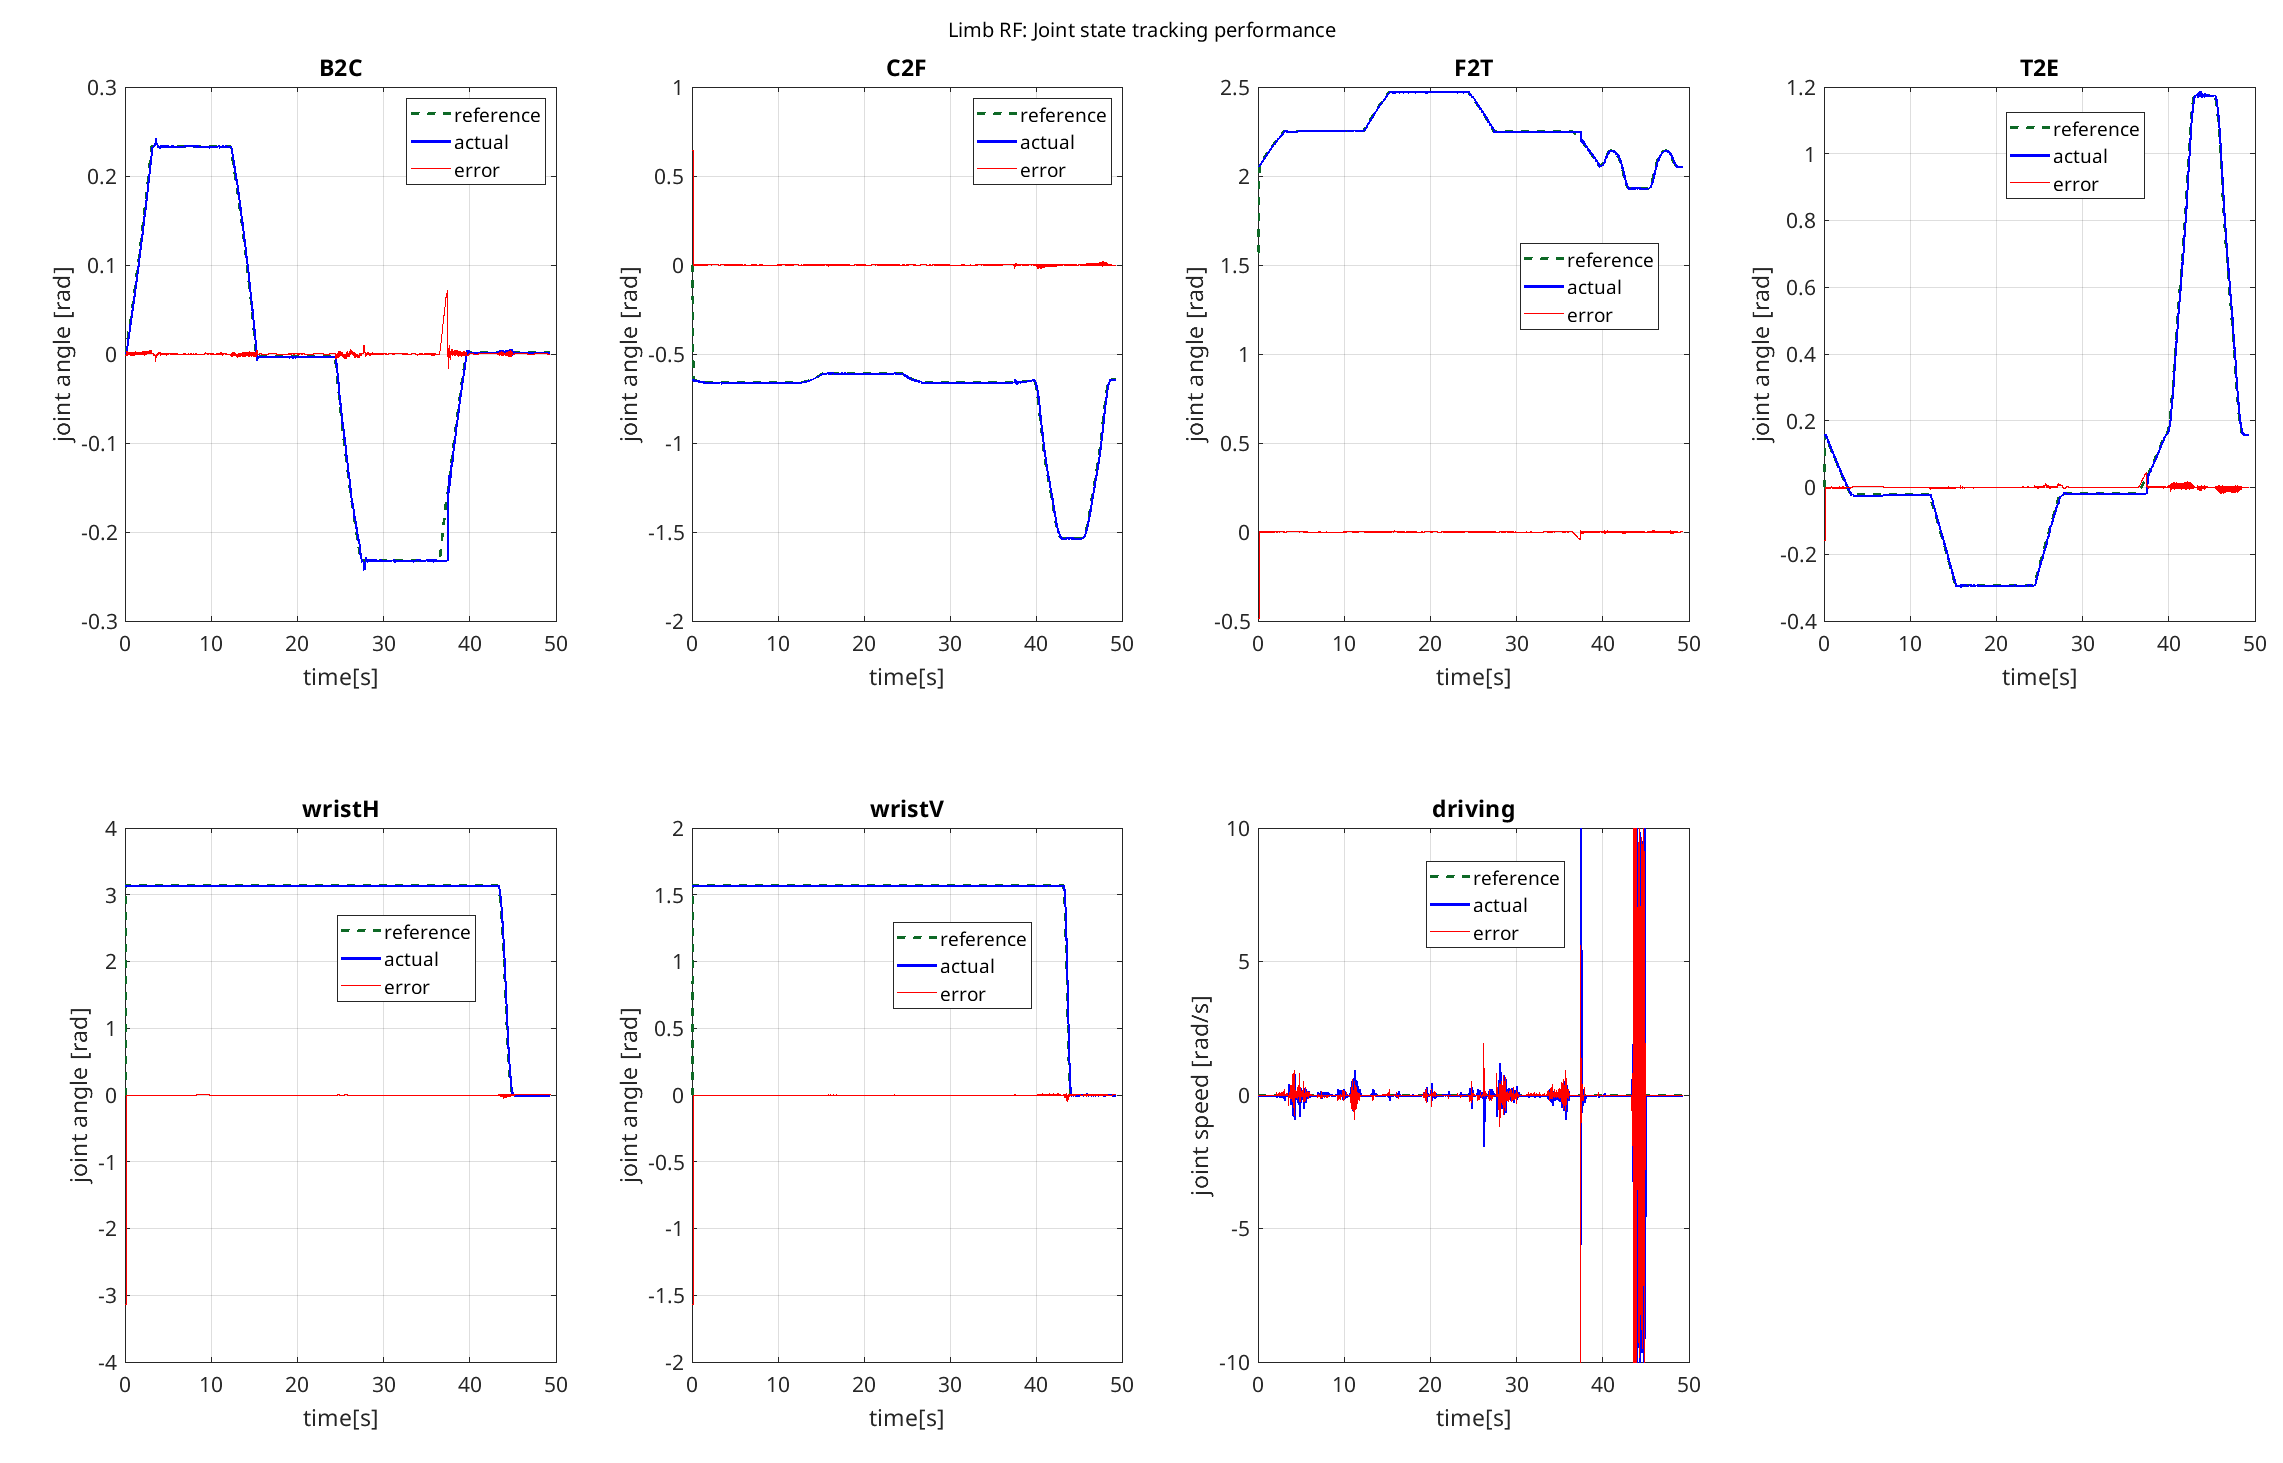
\includegraphics[width=1.0\textwidth]{Images/img_ch8/W2G_RF_joints.png}
    \caption{RF limb, Joint tracking during W2G}
    \label{fig:W2G_RF_harmonic_joint}
\end{figure}

\begin{figure}[H]
    \centering
    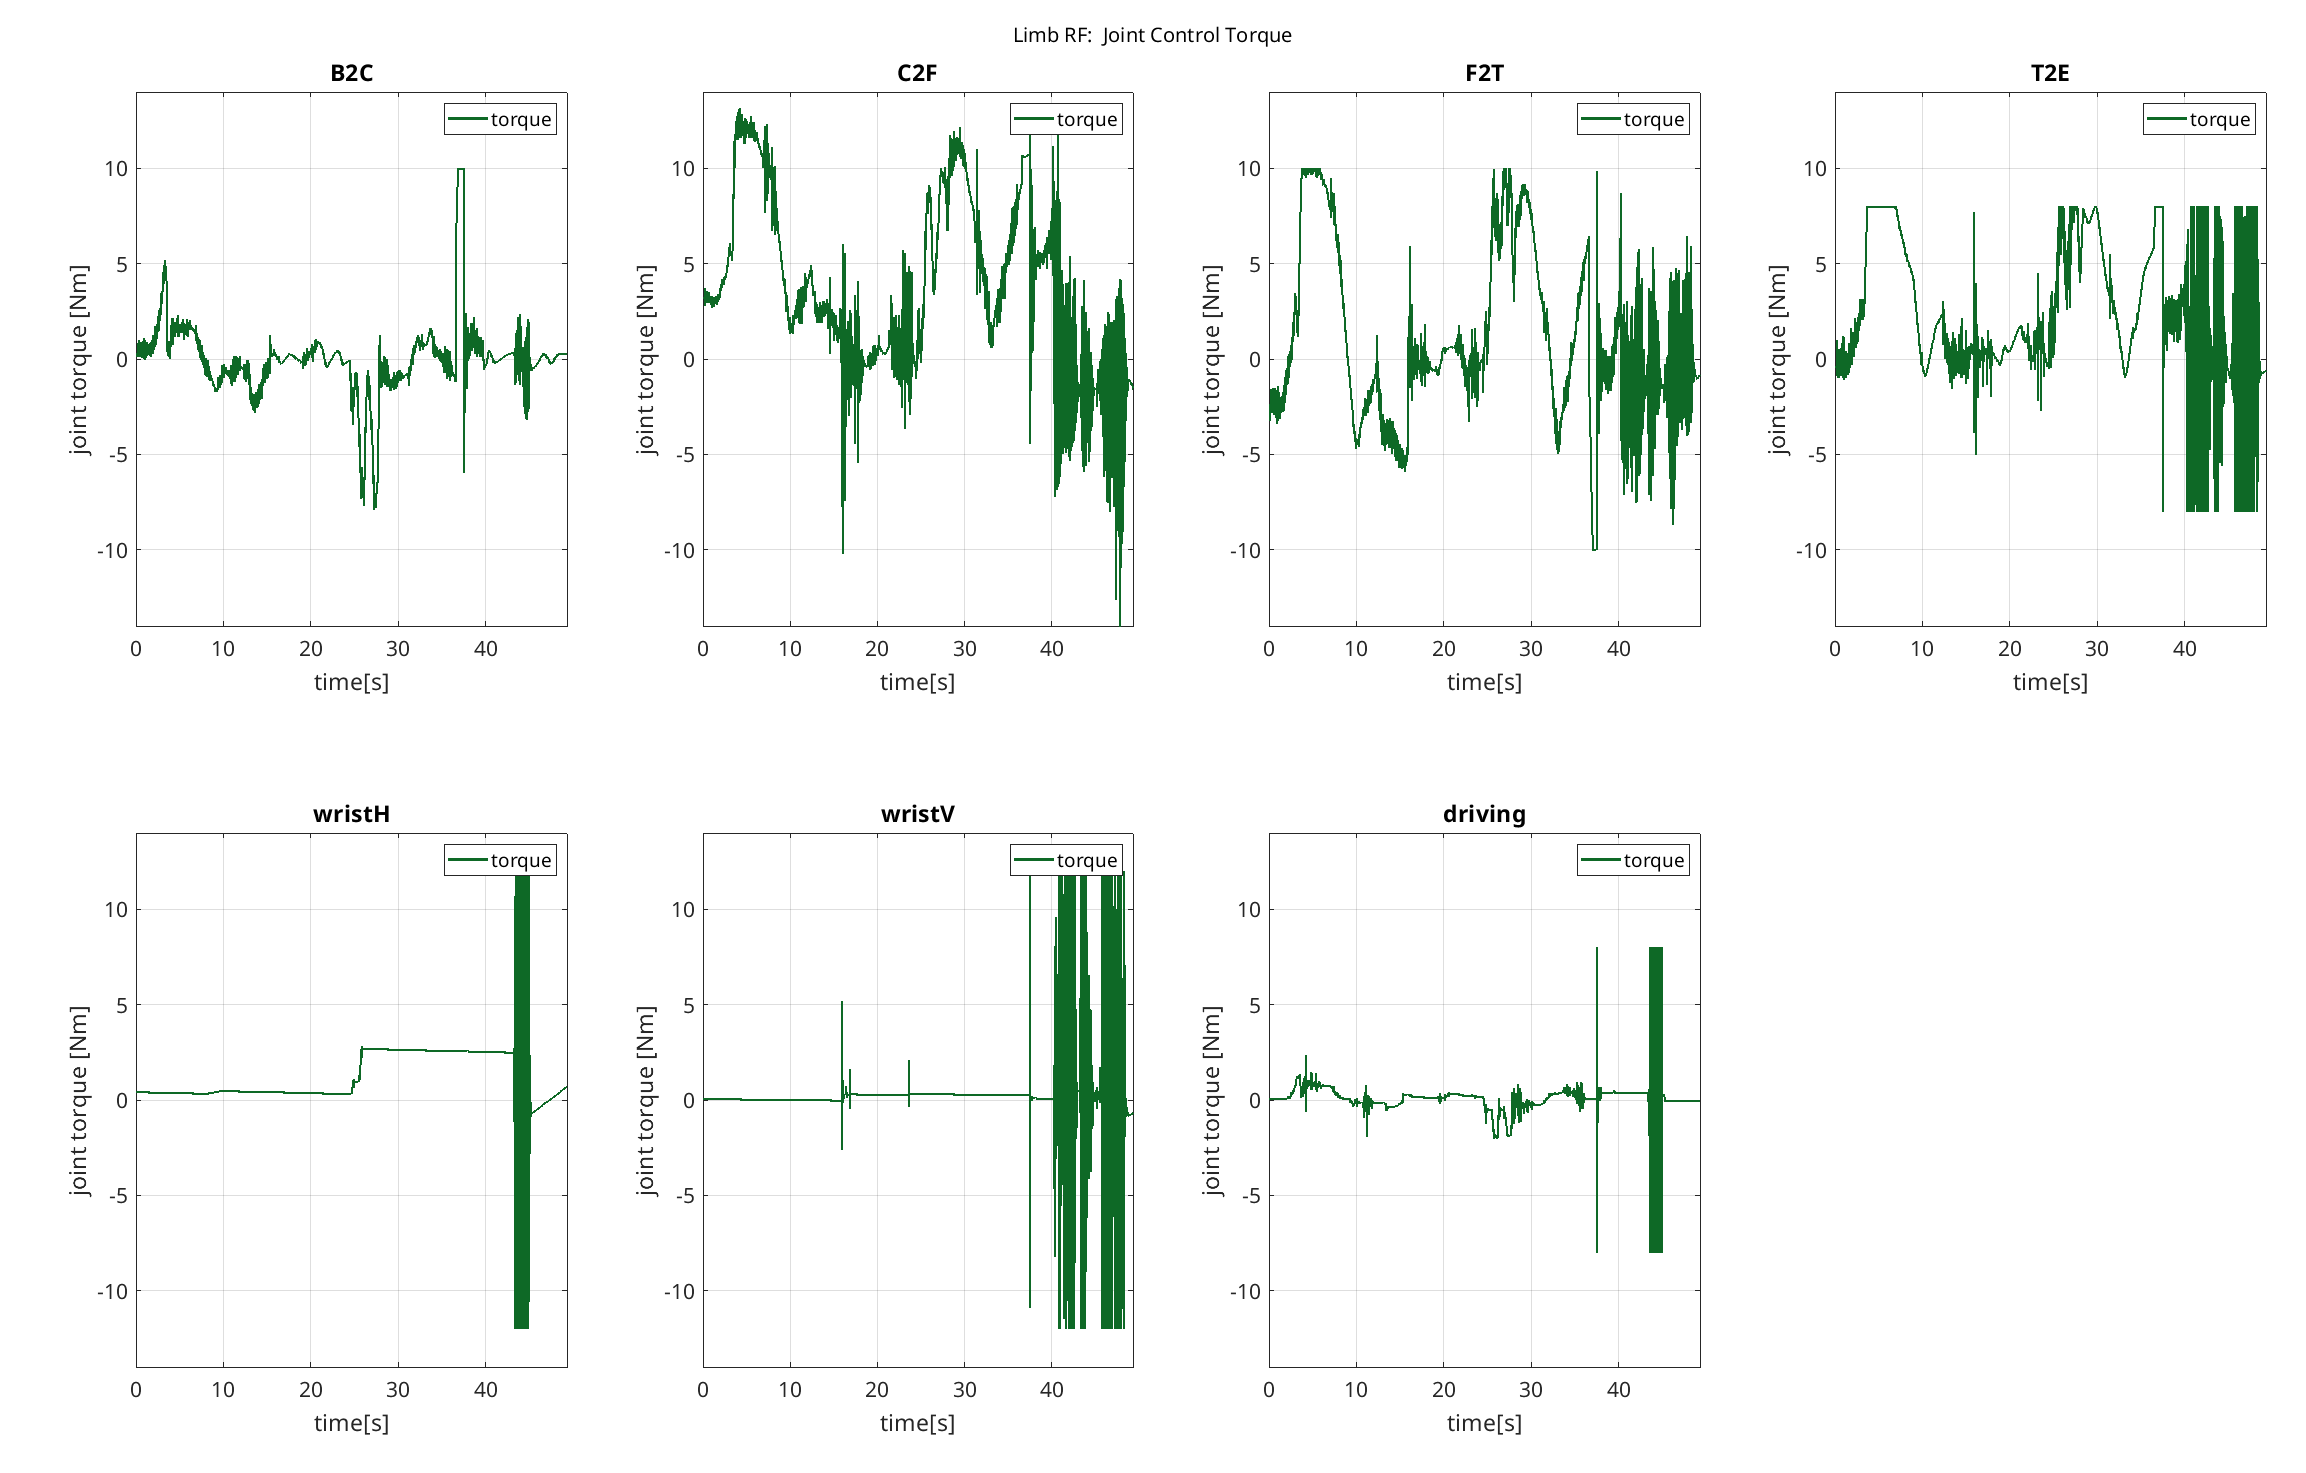
\includegraphics[width=1.0\textwidth]{Images/img_ch8/W2G_RF_torque.png}
    \caption{RF limb, Joint torques during W2G}
    \label{fig:W2G_RF_harmonic_torque}
\end{figure}

\begin{figure}[H]
    \centering
    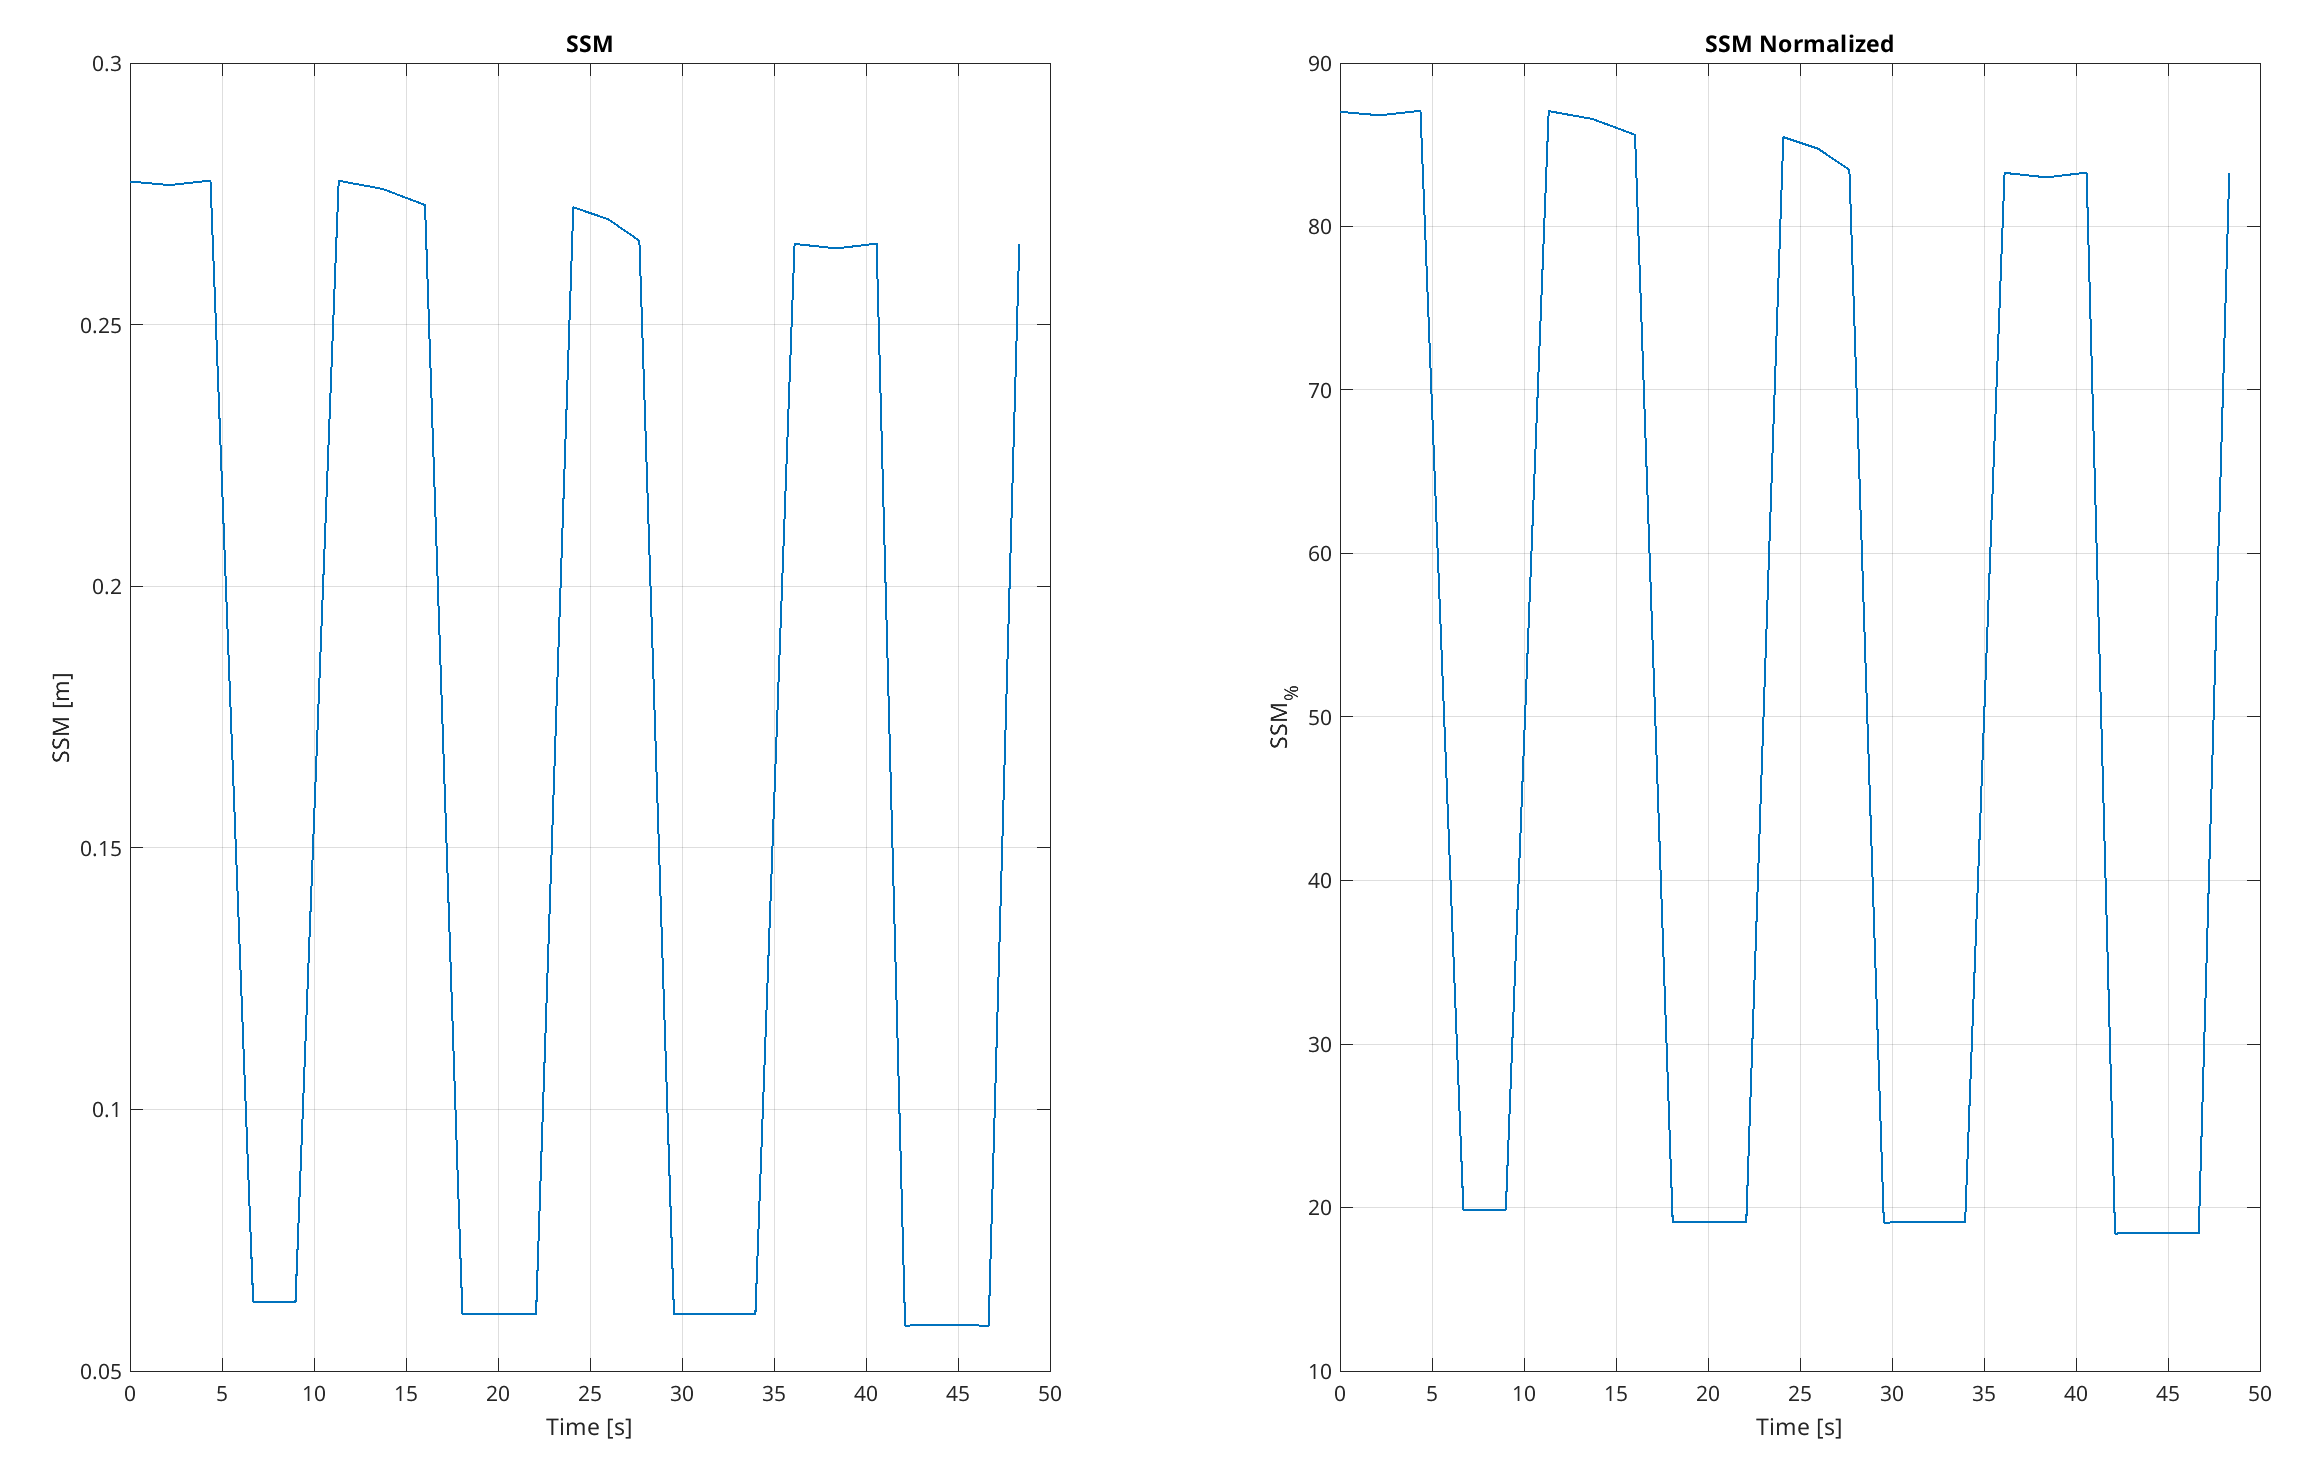
\includegraphics[width=0.9\textwidth]{Images/img_ch8/W2G_SSM.png}
    \caption{SSM and $SSM_\%$, during W2G}
    \label{fig:W2G_SSM_harmonic}
\end{figure}

\section{Discussion}
\label{sec:discussion}

The results presented in the previous section are now commented on, analyzing the motion controller and the transformation algorithm. Additional considerations on the system performances and the designed algorithms have been already discussed in the previous chapters. 

Limb controllers ensure satisfactory performances in terms of steady-state error and settling time. The average joint tracking error is kept below 0.05 rad in the real system, and 0.007 rad in simulation. Furthermore, in simulation, the maximum tracking error is always below 0.06 rad, while in the real system, the motors' mechanical limitations slow down the response time, with error picks for high slope set points signals (almost steps), but negligible steady-state error.    
Base motion, limbs motion, and GRIEEL transition tasks, teleoperated or computed autonomously by high-level algorithms, are correctly completed. 

The defined transformation algorithm ensures a stable and efficient motion sequence, as proven by the SSM analysis, conducted in the different testing environments.
In terms of stability, in fact, both in the real experiments and in simulation, the $SSM_\%$ is always higher than 18\%. The dexterity and conservativeness of motion are derived from the manipulability ellipsoid, which is maintained with the major axis parallel to the desired base motion. 

Because of hardware limitations, discussed in the next section, driving-to-walking mode transition cannot be completed in the real system experiments, and wheeled locomotion was not possible. Nevertheless, the simulation results prove that the designed motion controller architecture ensures smooth mode transition and driving locomotion. 

From the analysis of the simulator and the real system performance, it is possible to infer combined results.

In the \textbf{simulator}, the transformation sequence is executed as in the nominal design, and a realistic torque control profile is required both for the G2W and W2G transition. A redefinition of the motion tasks with longer execution time can be considered to reduce the joint torque requirements, that currently use high values. 
The wheeled locomotion on 3-wheels is less stable as can be deduced from the high frequency switching joint torque in the driving test. This information is useful for the future development of advanced control logic in wheel mode. 

In the \textbf{real system}, initial configuration, counterweight reliability, and hardware limitations affect the experiments. Nevertheless, in the motion sequences without failures, as the one reported in the previous section, a satisfactory base and limb motion is performed with the designed control system and motion algorithms. 

The estimated average time to complete the transition is around $240s$, which is the double of the previous transition sequence required time. This limitation is mainly caused by the single module transition in each transition step, in fact, each GRIEEL transformation takes on average $35s$. Therefore, half of the total transformation time consists of module transformation, previously executed in parallel.   

In conclusion, from the two testing environments, the designed control system and transition algorithm guarantee the defined requirements. 

\section{Limitations}
\label{sec:limitations}

To conclude the analysis of the conducted tests, the main limitations of the system and the testing environment are discussed here. 

\subsection{Hardware Limitations}
\label{sec:HW_limitations}

\subsubsection{Motors}
During the experiments on the real system motor failures and missing feedback information limits the system performances and achievable tasks. 

To analyze torque requirements, first, only gravitational load on joints has been estimated both with a serial link model and with a simplified mechanical structure. The model used for the estimation of gravity compensation effort when the limb supports the base is represented in Fig.\ref{fig:contact_payload}.

\begin{figure}[H]
    \centering
    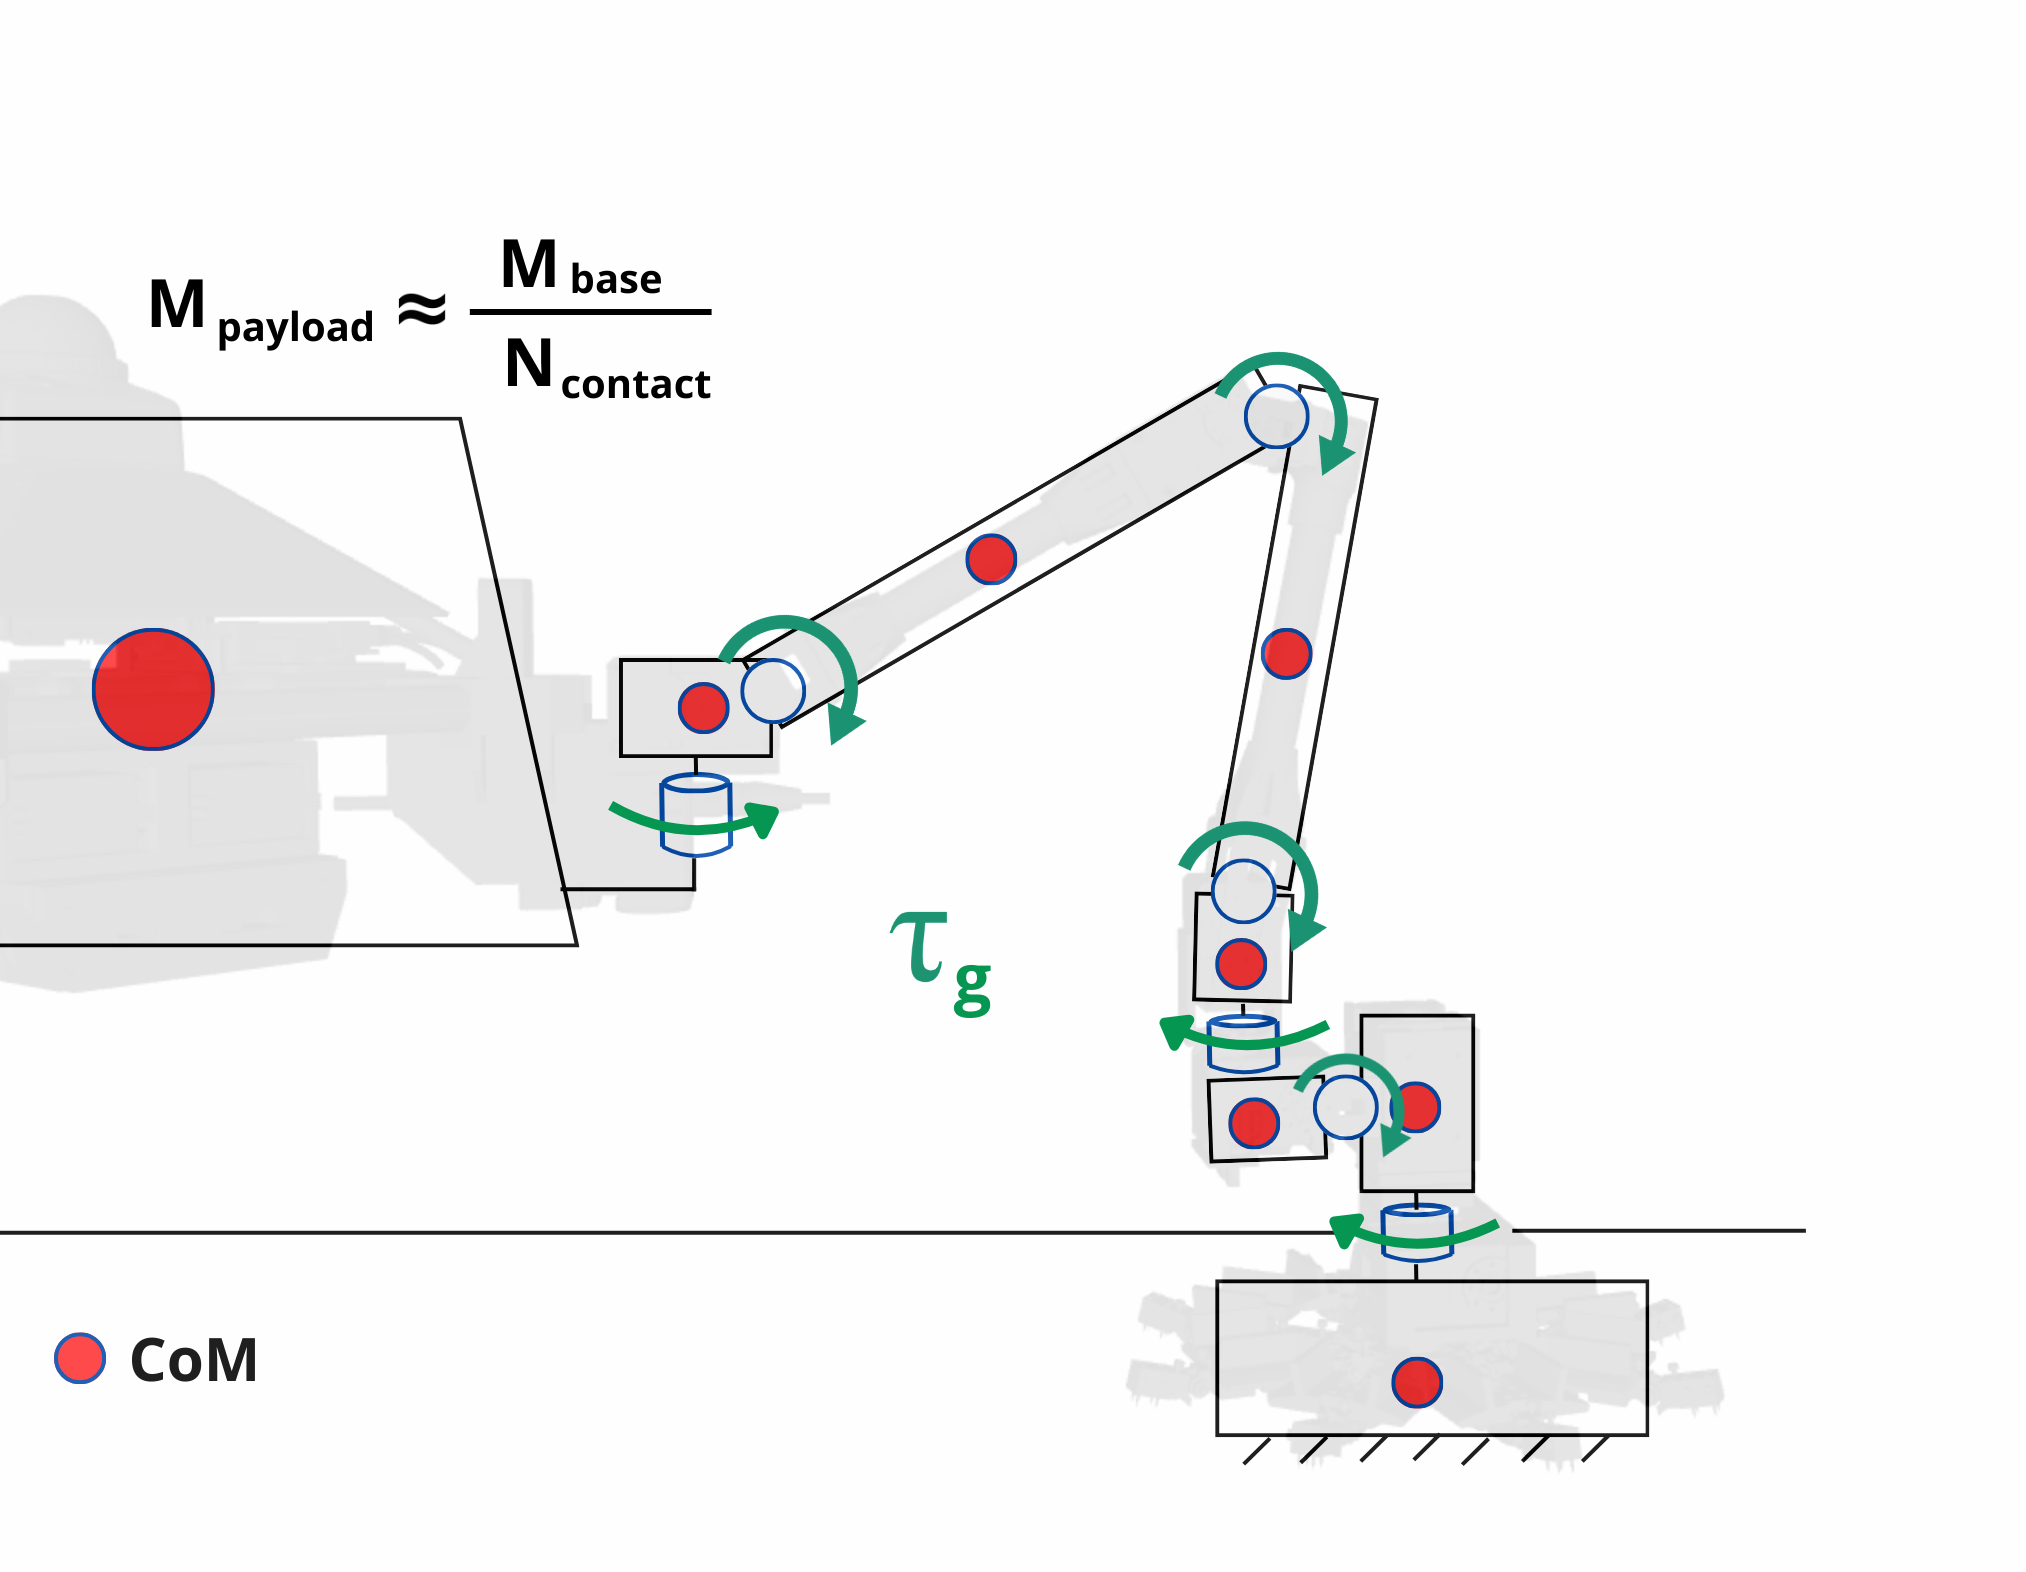
\includegraphics[width=0.65\textwidth]{Images/img_ch8/contact_payload.png}
    \caption{Limb model to estimate joints gravitational load}
    \label{fig:contact_payload}
\end{figure}

The results of this gravitational load analysis show that when supporting the base with $F2T = \pi/2 + \pi/6$ and $C2F = -\pi/6$ (the walking configuration), wristV motor is subject to a gravitational load of about $3Nm-4Nm$ in four/three limb support, and the same is for T2E and F2T (the other joints responsible for base support). 
Furthermore, when the limb is not in contact and the payload is considered the GRIEEL module, in the same configuration as before, the load is mostly on the F2T joint, around  $-2 Nm$ (holding torque is in the opposite direction).

Comparing these results with the motor datasheet (data reported on Tab.\ref{table:DYNAMIXEL}), it is evident that the current motors are not enough powerful to sustain the robot and complete motion tasks. This is further demonstrated by the laboratory experimental setup, which required the counterweight structure to avoid motor failures due to overload. 

\subsubsection{Sensors}

An additional system limitation is related to the available feedback information that can be used in the control architecture. 
In particular, the limb contact state and GRIEEL fingers' passive joint state have to be tracked to achieve autonomy.

One possible solution to retrieve this information is integrating sensors into the robot, and the lack of these has been a limiting factor during the experiments. 

\subsection{Controller Limitations}
\label{sec:control_limitations}

As will be discussed in detail in future work, the current limb controller can complete safe motion tasks only in nominal obstacle-free conditions. 

PID closed-loop joint control allows reaching the desired limb pose even in the presence of disturbances and additional inertial/gravitation load. However, when along the planned trajectory unexpected obstacles occur, compliance control and force-based motion controllers best fit these problems, which are common in unstructured environments.   

Even if the experiments have been conducted in a simple testing environment, when an unexpected base pose occurs, limb and base motion control loses accuracy and reliability. 

\subsection{Performance/Stability Index Limitations}
\label{sec:control_limitations}

In the evaluation of the robot's performance, stability and maneuverability with the new BME have been considered. 

The limitations of the BME have been already discussed, and are related to misleading satisfactory ellipsoid shapes in configurations not dexterous.
Moreover, the current stability evaluation based on the SSM is not reliable for such a complex system. From the experiments, it is not possible to derive the cause of some stability failure because motors limitation and unreliable counterweight also affects the results. Additional experiments and analysis are required to understand if the SSM-based transformation algorithm ensures stability also in the real system.


\subsection{Simulator Limitations}
\label{sec:control_limitations}

The configuration of the simulator involves a great effort to create a reliable Sim-to-real testing environment, but the complex gripper and wheel's grouser ground interaction is approximated and not 100\% accurate. The behavior from simulations is realistic, and a physics engine is integrated, but the approximation of real system behavior is involved. 
For those reasons, the results obtained from the simulation are important information for the system design and performance analysis, but unmodeled disturbances and dynamics create approximation errors. 